\documentclass[twocolumn,showpacs,preprintnumbers,nofootinbib,prd,
superscriptaddress,10pt]{revtex4-1}

\usepackage{amsmath,amssymb}
\usepackage{amsfonts}
\usepackage[normalem]{ulem}
\usepackage{textcomp}
\usepackage{hyperref}
\usepackage{enumitem}
\usepackage{bm}
\usepackage{afterpage}
\usepackage{graphicx}
\usepackage{psfrag}
\usepackage{mathtools}
%\usepackage{tensor}
\usepackage{layouts}
%\usepackage{DejaVuSans}
\usepackage{epstopdf}
\usepackage[usenames,dvipsnames]{xcolor}
\usepackage[utf8]{inputenc}
\usepackage{multirow}
\usepackage{rotating}
\usepackage{tabularx}
\usepackage{ragged2e}
\usepackage{blindtext}
\usepackage{graphicx}
\usepackage{siunitx}
	\sisetup{output-decimal-marker={.}}
\newtheorem{theorem}{Theorem}
\usepackage{float}
	

	%some math symbols
\newcommand{\R}{\mathbb{R}}
\newcommand{\N}{\mathbb{N}}
\DeclareMathOperator{\sign}{sign}
\renewcommand{\d}[1]{\ensuremath{\operatorname{d}\!{#1}}}
%argmin and argmax
\DeclareMathOperator*{\argmax}{arg\,max}
\DeclareMathOperator*{\argmin}{arg\,min}

% comments command
\newcommand{\wdp}[1]{{\textcolor{magenta}{\texttt{WDP: #1}} }}
\newcommand{\amartini}[1]{{\textcolor{blue}{\texttt{SS: #1}} }}
\newcommand{\sschmidt}[1]{{\textcolor{red}{\texttt{SS: #1}} }}

\begin{document}

	%%%%%%%%%%%%%%%%%%%%%%%%%%%%%%%%% ABSTRACT
\begin{abstract}
Burg method of Maximum Entropy Spectral Analysis (MESA) provides a powerful tool to perform spectral estimation of a time-series. The method is a generalization of Jaynes maximum entropy principle and provides the estimate for the spectrum in terms of the coefficients of some autoregressive process AR(p) or order $p$.
A closed form recursive solution provides an estimate of the autoregressive coefficients as well as of the order $p$ of the process.
We provide a ready to use implementation of the algorithm in the form of a python package `memspectrum`. We characterize our code performing a power spectral density analysis on some syntethic generated data (with known power spectral density) and we compare different criteria for stopping the recursion. Furthermore, we compare the performance of our code with the traditional Welch algorithm, using both syntethic data and real gravitational waves data from the LIGO-Virgo collaboration.
We find that, when compared to the Welch's method, the Burg's method provides a power spectral density (PSD) estimation with a systematically lower variance. This is particularly manifest in the case of a little number of datapoints, making Burg method most suitable to work in this regime.
%Several methods are characterized on synthetic noise having a known power spectral density (PSD) via the computation of the percentage error and then compared.  

\end{abstract}
	
	%%%%%%%%%%%%%%%%%%%%%%%%%%%%%%%%% TITLE
	\title{Maximum Entropy Spectral Analysis: a case study}
	\author{Alessandro \surname{Martini}}
		\email{martini.alessandr@gmail.com}
        \affiliation{Dipartimento di Fisica  Università di Pisa, and INFN Sezione di Pisa, Pisa I-56127,Italy}        
	\author{Stefano \surname{Schmidt}}
		\email{s.schmidt@uu.nl}
        \affiliation{add me}      
	\author{Walter \surname{Del Pozzo}}
		\email{walter.delpozzo@unipi.it}
        \affiliation{Dipartimento di Fisica  Università di Pisa, and INFN Sezione di Pisa, Pisa I-56127,Italy}      
  
	
	\maketitle
	\tableofcontents

	%%%%%%%%%%%%%%%%%%%%%%%%%%%%%%%%% BODY  

\section{Introduction}

The study of the properties of  stochastic processes is a crucial task in many fields of physics and mathematical physics [Here we should make some examples...].
A particularly interesting class of stochastic processes are the so-called \textit{wide-sense} stationary processes. These are stochastic processes that display an invariance of their statistical properties, such as their two-point autocovariance function, with respect to time translation. If $x(t)$ is a wide-sense stationary process, it is completely determined by the knowledge of the auto-covariance function 
\begin{equation}
	C(\tau) = \mathbf{E}[x_t \cdot x_{t+\tau}]
\end{equation}
or equivalently by the knowledge of their \emph{power spectral density} (PSD) $S(f)$. Thanks to the Wiener-Khinchin theorem the two are related by a Fourier transform: 
\begin{equation}
	S(f) = \int_{-\infty}^{\infty} \textrm{d}\tau C(\tau) e^{-i 2 \pi f \tau}\,.
\end{equation}
In some literature, the PSD is introduced as  
\begin{equation}\label{eq:psd-f-definition}
	\mathbf{E}[\tilde{x}(f) \cdot \tilde{x}(f^\prime)] = S(f) \delta(f-f^\prime)
\end{equation}
without highlighting its connection with the time structure of the process itself, thus masking some important properties that will explore further in what follows. The latter definition in (\ref{eq:psd-f-definition}) gives, however, i) a straightforward interpretation of the PSD: it measures how much signal ``power" is located in each frequency; ii) an operative way of estimating it for an unknown process.  
%Under such assumption, it can be shown [cite something] that the problem of characterizing the noise properties is greatly simplified and its properties are summarized by a single \textit{autocorrelation function}, which describes how an observation at a given time correlates with another observation a later time. More formally, the properties of a zero mean time series $x_t$ are described by the function:
%\begin{equation}
%	R(\tau) = \mathbf{E}[x_t \cdot x_{t+\tau}]
%\end{equation}
%where the average is computed on different times $t$.
%Thus, a stationary noise time series is completely characterized by the autocorellation function.
%\par
%More often, the study is performed in frequency domain: indeed, for stationary noise the components in frequency $\tilde{x}(f)$ of a stationary time series are conditionally independent from each other. It can be shown that:
%\begin{equation}
%	\mathbf{E}[\tilde{x}(f) \cdot \tilde{x}(f^\prime)] = S(f) \delta(f-f^\prime)
%\end{equation}
%This equation defines the function \textit{power spectral density} (PSD) $S(f)$.
%The PSD has a straightforward interpretation: it measures how much signal ``power" is located in each frequency bin. Furthermore, it is not difficult to show that it is the Fourier transform of the autocorrelation function:
%\begin{equation}
%	S(f) = \int_{-\infty}^{\infty} \textrm{d}\tau R(\tau) e^{-i 2 \pi f \tau}
%\end{equation}
%A power spectral density fully describes a stationary noisy time series and this shows how important is in the study of noise.
%\par
%Thus, in many real application, the knowledge of the PSD is crucial for the understanding of the process and indeed algorithms for PSD computation are a standard part of every software package for computational physics.
A ubiquitous method for such computation is due to Welch \cite{Welch} and it based on the method of periodograms. Basically, the PSD is obtained by slicing the observed realisation $x(t_1),\ldots,x(t_n)$ of the process $x(t)$ into many windowed batches and averaging the squared moduli of their Fourier transforms. The standard approach of periodograms \cite{Lomb,Scargle} consists in taking the Fourier Transform of the sample autocorrelation, written as \begin{equation}
    \rho = \left\{W_0\rho_0,W_{\pm 1}\rho_{\pm 1}, \dots, W_{\pm M}\rho_{\pm M}, 0, 0, \dots \right\}.
\end{equation}
The sequence $W$ is a window function that can be chosen in several different way, each choice presenting advantages and disadvantages for the final estimate of the PSD. \\ 
The choice of a window function is arbitrary and typically is made by trial and error, until a satisfactory compromise between variance and resolution of the estimate of PSD is reached. A high frequency resolution implies high variance and vice-versa. Moreover, the final result depends on the choice of window function, hence begging the question of what the ``real" PSD is. \\  
Another problem with this approach is the requirement for the window to be $0$ outside the interval: we are arbitrarily assuming $\rho_j = 0$ for $j > M$, and modifying the estimate if a non-rectangular window is chosen. Making assumptions on unobserved data and modifying the ones we have at our disposal introduces information about the process that is not really there. Moreover, this method requires a number of arbitrary choices to be made, e.g. the number of time slices, the kind of Window function, the overlap between consecutive slices, etc... All the knobs must be tuned by hand and their choice can dramatically affect the PSD estimation.
\par
An appealing alternative approach, based on the Maximum Entropy principle \cite{Jaynes}, has been put forward by Burg \cite{burg1975maximum}. Being rooted on solid theoretical foundations, we will see that Burg's method, unlike Welch's, does not require any preprocessing of the data and requires very little tuning of the arbitrary parameters, as it provides an iterative closed form expression for the spectrum of a stochastic time series. Furthermore, it embeds the PSD estimation problem into an elegant theoretical framework and makes minimal assumptions on the nature of the data.
Lastly and most importantly, it provides a robust link between spectral density estimation and the field of autoregressive processes. This provide a natural and simple machinery to forecast a time series, thus predicting past observations based on previous ones.
In this paper we discuss the details of the Maximum entropy principle, its application to Power Spectral Density estimation with Burg algorithm and the link between Burg's algorithm and autoregressive process. Furthermore, we present and describe a new code, `memspectrum`, that provides a robust python implementation of the algorithm.
We provide a thorough assessment of the performance of our code and we validate our results performing a number of tests. We compare our results with those of spectral analysis carried out with the standard Welch method.
\par
Our paper is organized as follows: blablabla...


\section{Theoretical foundations}
The Maximum Entropy principle (MAXENT) is among the most important results in Bayesian probability theory. It provides a way to uniquely assign probabilities to a phenomenon in a way that best represent our state of knowledge, while at the same time it is non committal with unavailable information. Its domain of application turned out to be wider than expected. In fact, thanks to Burg \cite{burg1975maximum}, this method has also been applied to perform high quality computation of power spectral densities of time series.

After a short introduction to Jayne's MAXENT (sec.~\ref{sec:MAXENT}), we will develop in detail Burg's technique of Maximum Entropy Spectral Analysis (MESA) and show that the estimate can be expressed in an analytical closed form (sec.~\ref{sec:MESA}).
Next, we will discuss an interesting link between Burg's method and autoregressive processes (sec.~\ref{sec:autoregr}) and in sec.~\ref{sec:forecasting} we will use such link to introduce a method for forecasting a time series.

\subsection{Maximum Entropy Principle} \label{sec:MAXENT}

Before introducing MAXENT as a variational problem, we will workout some simple examples to contexualise how information's entropy
and `uncertainty' are related. First of all,  it is worth noting that the word `information' will not be used to indicate our knowledge on the system under study: this is what we will call `evidence'. Information will be intended as in communication theory: it specifies the length of the message necessary to provide
a full description of the system under study.

For instance, consider a perfectly sinusoidal signal: knowledge of amplitude, frequency and phase are sufficient to fully reproduce it: 
it has a low information entropy content. Even less information is required if we are studying a system whose outcome is 
certain (has probability $p = 1$). If the amount of information $I$ can be considered to zero, a communication is not even needed.  
Shannon \cite{Shannon} proposed the quantity
\begin{equation}\label{eq:information}
    I = \log_2 \frac{1}{p(x)}
\end{equation}
to represent the quantity of information brought by an outcome $x$ with probability $p(x)$. It is additive quantity as well as monotonically decreasing as a function of $p \in [0, 1]$. The more uncertain the outcome, the higher the information it brings.
\par
What happens if we consider a larger set of different events? What is  the `most uncertain' outcome?  Since we are intending probability as a representation of the state of knowledge, one of the first requirement for our assignment is the agreement with common sense.
Consider an experiment based on the occurrence of one of two different outcomes $E_1, E_2$ with given probabilities $P_1$ and $P_2$. What are the values that make our outcome the most uncertain?
If $P_1$ and $P_2$ are largely different, like $P_1 = 0.999$ and $P_2 = 0.001$, we have enough evidence to believe that event $E_1$ will occur almost certainly, considering $E_2$ to be a very implausible outcome.
The most unpredictable experiment is the one in which 
\begin{equation}\nonumber
    P_1 = P_2 = \frac{1}{2}:
\end{equation}
this describes a situation of `maximum ignorance'; we have no evidence at all and we have no way of predicting what the outcome of such an experiment will be.  The generalisation to $N$ possible outcomes is straightforward. \\ 
%This can be generalized in the case of $N$ events. Assigning same probability
%\begin{equation*}
%    P_1 = \dots = P_N = \frac{1}{N}
%\end{equation*}
%for each outcome, i.e. appealing to the indifference principle (IP), is equivalent to the requirement for our experiment to be the most unpredictable. 
%All we know is that one over $N$ events is going to happen. With this evidence, we cannot expect one outcome to occur over the others. 
%To report the results of such an experiment, we need to communicate every single outcome: it 'carries' high information. 
In this context, the role played by evidence should also be clear: it dictates the probability assignment in order to make the result 'more certain' or 'less informative'. Any assignment different from the 'most uncertain' is violating the principle of it to being non committal to non-available evidence. We can only assign a more certain probability, i.e. less informative, if we have evidence for it. If we have none, the result has to be the most unpredictable, i.e. the most informative. From the point of view of communication theory: the higher the evidence on a system, the lower the information I need to send to describe it.
\par
MAXENT ratifies the aforementioned principle by stating that probabilities should be assigned by maximizing uncertainty using evidence as constraint. 
This defines a variational problem, where a numerical measure of uncertainty $H\left[p_1, \dots, p_N\right]$ has to maximized. $H$ has to be a 'generalization' of information defined in equation (\ref{eq:information}) to be something like the 'expected information' brought by an experiment with $N$ possible outcomes each with its own probability $p_i$.
%
%Some properties for $H$ can be worked out easily. 
%From previous discussion, given a fixed number $N$ of possible outcomes, we want $H$ to be maximized by the choice $p_1 = \dots = p_N$.
%Consider now the opposite situation, in which probability is assigned appealing to IP and we have a different number of possible outcomes.
%Intuitively, the most unpredictable experiment is the one with larger number of outcomes: probability of "getting it wrong" increases as $\frac{N -1}{N}$. So when equal probabilities are assigned, we want
%\begin{equation}
%    \nonumber
%    H\left[\frac{1}{N}, \dots, \frac{1}{N}\right]
%\end{equation}
%to increase monotonically with N.
%
%We also want our function to be continuous in its parameters: any small change in probability has to slightly affect uncertainty. \\
%Last is composition property. Consider three events with probability $p_1, p_2, p_3$ such that $p_2 + p_3 = 1 - p_1 = q$. We require 
%\begin{equation}
%    H\left(p_1, p_2, p_3\right) = H(p_1, q) + qH\left(\frac{p_2}{q}, \frac{p_3}{q}\right),
%\end{equation}
%so that uncertainty is additive.

Shannon \cite{Shannon} showed that the only functional form satisfying continuity with respect to its parameters and additivity is:
\begin{equation}\label{eq:entropy}
    H[p_1, \dots, p_N] = - \sum_{i = 1}^N p_i\log{p_i},
\end{equation}
or, in the continuous case:
\begin{equation}
    H[p(x)] = - \int p(x)\ln p(x) dx,
\end{equation}
and $H$ is what we will call (information) entropy.

The maximisation of entropy, supplemented by evidence in the form of constraints to which the sought-for probability distribution must obey,
gives rise to several of the most common probability distributions utilised commonly by data scientists. For instance, whenever the only constraint available is the normalisation of the probability distribution, the entropy is maximised by the uniform distribution. 
If the information available is instead the expected value -- the mean -- entropy is maximised by the  exponential distribution. Of particular importance is 
the case in which, in addition to the mean, also the variance is known. MAXENT leads to the Gaussian distribution. 
We retain this particularly interesting from the foundational point of view, since it provides a deeper insight into the ubiquitous Gaussian distribution.
It is not only the limit distribution provided by the central limit theorem for finite variance processes but it is also the distribution that maximizes the entropy. For this reason, appealing to MAXENT principle, it is the correct assignment if mean and covariance are the only quantities that fully define our process. In some sense, we can interpret the central limit theorem as the natural `statistical' evolution toward a configuration that maximizes entropy. 

For this work, we are particularly interested in the mutli-dimensional case. Suppose we have a vector of measurements $(x(t_1),\ldots,x(t_n)) = (x_1, \ldots, x_n)$ that we conveniently express as a single realisation of an unknown stochastic process $x(t)$ and we have information about the expectation value of the process $\mu(t)$ and on the matrix of auto-covariances $C_{ij} \equiv C(t_i,t_j)$, then the MAXENT distribution is the $n$-dimensional multivariate Gaussian distribution\cite{gregory_2005}: 
\begin{align}
    p&\left((x_1, \ldots, x_n)\vert I\right) = \nonumber \\
    &\frac{1}{\left(2 \pi \det C\right)^{k / 2}}\exp\left(-\frac{1}{2}\sum_{i,j}(x_i-\mu_i) (x_j-\mu_j)C^{-1}_{ij} \right)\,. 
\end{align}
We have already seen that for a wide-sense stationary process the mean function is independent of time, hence redefined to be equal to zero without loss of generality, and the auto-covariance function is dependent only on the time lag $\tau \equiv t_i - t_j$. One can thus choose a sampling rate $\Delta t$ so that $C_{ij} = C((i-j)\Delta t)$. The autocovariance matrix thus becomes a Toeplitz matrix. Toeplitz matrices are asymptotically equivalent to circulant matrices and thus diagonalised by the discrete Fourier transform base\cite{Gray}.
%R. M. Gray, Foundations and Trends⃝R in Communications and Information Theory 2, 155 (2005), URL https://doi.org/10.1561/0100000006.
Some simple algebra shows that the time-domain multivariate Gaussian can be transformed into the equivalent frequency domain 
probability distribution:
\begin{align}
p&\left((\tilde{x}_1, \ldots, \tilde{x}_n)\vert I\right) = \nonumber \\
    &\frac{1}{\left(2 \pi \det S\right)^{k / 2}}\exp\left(-\frac{1}{2}\sum_{i}(\tilde{x}_i^2S^{-1}_{i} \right)\,,
\end{align}
where the matrix $S$ is an $n\times n$ diagonal matrix whose elements are the PSD $S(f)$ calculated at frequency $f_i$.
Many readers will recognised the familiar form of the Whittle likelihood that stands at the basis of the \emph{matched filter} method\cite{woodward}
%P. M. Woodward, D. W. Fry, and W. Higinbotham, Probability and information theory, with applications to radar; 2nd ed. (Pergamon Press, Oxford, 1964), URL http://cds.cern.ch/record/2031792.
and of gravitational waves data analysis, e.g. \cite{finn:1992}.
% L. S. Finn, Phys. Rev. D46, 5236 (1992), gr-qc/9209010
Thanks to MAXENT, the problem of defining the probability distribution describing a wide-sense stationary process is thus 
entirely reduced to the estimation of the PSD or, equivalently, the auto-covariance function.

%
%

%This interpretation is straightforward: if we compare it with Eq.~(\ref{eq:information}), we see that the entropy is defined as the 'average information'. The probability assignments made maximizing it with respect to $p$, is somehow requiring  the 'expected value' of uncertainty to be a maximum. Such an assignment is in agreement with our hypothesis of being `non committal' with unavailable evidence, since \ref{eq:entropy} is all we need to assign probabilities uniquely. Evidence can be added in form of constraints in the maximization.

%It is easy to verify that this expression for entropy verifies the aforementioned properties. 
%Assigning the same value for each probability $p_i$, it is straightforward to verify $H$ increases with N: 
%\begin{equation}
%    -\sum_{i = 1}^N \frac{1}{N}\log{\frac{1}{N}} = - \log\frac{1}{N} = \log N.
%\end{equation}
%\wdp{I need to review and correct the following}
%To show how the maximization of entropy, supplemented with additional evidence, can provide a unique probability assignment, 
%we use a simple, pedagogical example. Consider the case in which we want assign a probability distribution $p(x)$ to a variable $x$ 
%for which we know mean $\mu$ and covariance $\Sigma$. Our `evidence' is then coded as the following constraints:
%\begin{align}
%\sum_{i = 1}^{N}p_i &= 1 \\
%\sum_{i = 1}^{N}x_i p_i &= \mu \\
%\sum_{i = 1}^{N}(x_i - \mu)(x_j - \mu) p_i &= \Sigma\,
%\end{align}
%where the first row states the requirement of exhaustivity.
%\wdp{i think we want the multivariate case since i) the gaussian case is also on wikipedia ii) we actually will need that  later on.}

%First of all, we want to show that, in case in which our only constraint is exhaustiveness
%$\sum_{i = 1}^{N}p_i = 1 $,
%MAXENT reduces to indifference principle as it should be. The variational problem is defined as
%\begin{equation}\label{eq:entropyNormConst}
%    \delta\left[H - \lambda\sum_{i = 1}^N (p_i - 1)\right] = 0 
%\end{equation}
%with
%\begin{equation}
%    \delta H\left[p_1, \dots, p_N\right] = \sum_{i = 1}^N\frac{\partial H}{\partial p_i}\delta p_i = - \sum_{i = 1}^N\left(\log p_i + 1\right),
%\end{equation}
%so that equation \ref{eq:entropyNormConst} reduce to
%\begin{equation}\nonumber 
%    \sum_{i = 1}^N\left[\log p_i + \lambda + 1 \right]\delta p_i = 0\,.
%\end{equation}
%The solution of the previous equation is easily worked out requiring every term to be zero: 
%\begin{equation}\nonumber 
%    p_i = e^{-\lambda - 1}.
%\end{equation}
%Applying the normalization condition, it is immediate to show that
%\begin{equation}
%    p_i = \frac{1}{N}.
%\end{equation}
%MAXENT reduces to the IP when only the normalization constraint is used.
%
%In the second example, we will add the constraint that the distribution has a known mean value: $\int \d{x} x p(x) = \bar{x}$. For simplicity we will work in the continuous case.
%The variational problem can be rewritten as: 
%\begin{equation}
%    \int \left[\log p(x) + 1 + \lambda + \mu x \right]\delta p(x) = 0
%\end{equation}
%with constraints: 
%\begin{equation*}
%    \int \d{x} \; p(x)  = 1 \text{  and  }
%    \int \d{x} \; x p(x) = \bar x.
%\end{equation*}
%For simplicity, we consider $x$ to be a variable ranging in the interval $(-\infty,+\infty)$, but this can be easily computed for every other interval.
%
%The general solution for $p(x)$ is:
%\begin{equation}
%    p(x) = e^{-1 - \lambda - \mu x} 
%\end{equation}
%where $\lambda$ and $\mu$ are two Lagrange multipliers
%The normalization conditions implies 
%\begin{equation}\nonumber 
%   1 =  \int \d{x} \; p(x) = e^{-1-\lambda}\int e^{-\mu x} dx, 
%\end{equation}
%so that: 
%\begin{equation}\nonumber 
%    e^{-1 -\lambda} = \mu.
%\end{equation}
%The fixed average condition provides a value for $\mu$ in terms of $\bar{x}$:
%\begin{equation}
%	\mu = \frac{1}{\bar{x}}
%\end{equation}
%The solution is then an exponential distribution:
%\begin{equation}
%    p(x) = \frac{1}{\bar{x}} \exp\left(-\frac{x}{\bar{x}}\right). \nonumber 
%\end{equation}
 
%Lastly, and more interestingly, we also consider a constraint on the variance. For this reason, we set:
%\begin{align*}
%    \int \d{x} \; p(x)  = 1 \text{  and  }
%	\int \d{x} \; x p(x) = \bar{x} \\
%	\text{  and  }
%	\int \d{x} \; (x-\bar{x})^2 p(x)  = \sigma^2
%\end{align*}
%Performing the same computation as above, we obtain a well known result:
%\begin{equation}
%	p(x) = \frac{1}{\sigma\sqrt{2\pi}} e^{-\frac{1}{2}\left(\frac{x-\bar{x}}{\sigma}\right)^2}
%\end{equation}
%
%Take a vector  $\vec x(t)$ with components in $\mathbb{R}^N$
%\begin{equation*}
%    \vec x(t) = \left(x_1, \dots, x_N \right), \quad \text{ with } x_i = x(t_i),
%\end{equation*}
%We assume $\vec x$ to be time dependent and real valued because we will work with time dependent single channel signals. If we put constraints in both mean $\vec \mu(t)$ and covariance matrix $C_(t_i, t_j)$, MAXENT allow us to assign for $\vec x(t)$ a multivariate normal distribution \cite{gregory_2005}: 
%\begin{align}
%    p&\left(\vec x(t)\vert I\right) = \nonumber \\
%    &\frac{1}{\left(2 \pi \det C\right)^{k / 2}}\exp\left(-\frac{1}{2}\sum_{i,j}(x_i-\mu_i) (x_j-\mu_j)C^{-1}_{ij} \right). 
%\end{align}



\subsection{Maximum Entropy Spectral Analysis} \label{sec:MESA}

In principle, if the autocorrelation was known exactly (i.e. at every time $\tau \in (-\infty,+\infty)$), the computation of the PSD 
would reduce to a single Fourier transform.
However, in any realistic setting, we are dealing with a finite number of samples $N$ from the process, hence such computation
is impossible.
Moreover, the error $\sigma_k$ in the estimate of the autocorrelation after $k$ steps increases with $k$ as $\sigma \sim 1/\sqrt{N - k}$, so that only a few values for the autocorrelation function can actually be computed reliably.
This bring us the core of the problem: how to give an estimate from partial (and noisy) knowledge of the autocorrelation function? MAXENT can guide use in this task without any a priori assumptions on the unavailable data\footnote{Indeed this is the largest difference with the most common Welch method. The latter assumes that the unknown values of the autocorrelation are $0$. Clearly, this assumption is unjustified and MAXENT is a good way to drop this assumption.}.
\par
As in the previous examples, one needs to set up a variational problem where the entropy, Eq.~(\ref{eq:entropy}), is maximized 
subject to some problem-specific constraints. 
In our case, they are i) the PSD estimate has to be non-negative; ii) its Fourier transform has to match the sample autocorrelation (wherever an estimate of this is available).
\par
Before doing so, there is a technical problem to solve: the definition of entropy (Eq.~\ref{eq:entropy}) depends on a probability distribution, 
not on the PSD. The variational problem can be formulated in terms of the power spectral density $S(f)$ alone by
considering our signal as the result of filtering a white noise process with a filter whose power response is exactly $S(f)$ \cite{AblesMESA}. 
The entropy gain obtained by filtering white noise is: 
\begin{equation}\label{eq:EntropyGain}
    \Delta H = \int_{-\infty}^{\infty}\log S(f) df , 
\end{equation}
hence the variational problem can be stated by requiring that $S(f)$ maximises the entropy gain \sschmidt{Non ho capito questa parte...:(}. 
Time-limited observations do not provide access to the full frequency range, but only between minus and plus the Nyquist frequency, 
that, in turn is given by the sampling interval $\Delta t$ as $Ny \equiv \frac{1}{2 \Delta t}$. Hence, the finite-size entropy
gain is 
\begin{equation}\label{eq:EntropyGain2}
    \Delta H = \int_{- Ny}^{Ny}\log S(f) df\,.
\end{equation}

Consider a realisation of a stochastic process $(x_1,\ldots,x_n)$ with sample autocorrelations $\bar r_i,\,i=0,\ldots, n/2$, we require that the variational solution $S(f)$ for the PSD matches the empirical autocorrelation:
\begin{equation}\label{eq:MaxConstraint}
\int_{-Ny}^{Ny} S(f) e^{\imath 2 \pi f n \Delta t} df = \bar r_{n}\,.
\end{equation}
This approach on power spectral density estimate was developed by Burg \cite{burg1975maximum} and it is a way out from the problems raised in periodograms estimate. It requires no assumptions on the unavailable estimates for $\bar r_n$ and is consistent with the sample autocorrelation function by construction. Remarkably, the variational problem admits a closed-form analytical expression for $S(f)$:

\begin{equation}\label{eq:MESApsd}
    S(f) = \frac{P_N \Delta t}{\left(\sum_{s=0}^N a_s z^s\right)\left(\sum_{s = 0}^N a^*_s z^{-s}\right)}, 
\end{equation}
with $\Delta t$ the sampling interval, $z=\exp{(2\pi i f\Delta t)}$, $a_0$ = 1 and the coefficients $P_N$ and $a_i (i \neq 0)$ to be determined. The details of the derivation and the actual values of the coefficients $a_i$ can be found in appendix \ref{sec:MESA_solution}.

\subsection{Autoregressive Process Analogy} \label{sec:autoregr}

The application of MESA is not limited to spectral estimates, but it also provides a link between spectral analysis and the study
of autoregressive processes.\cite{doi:10.1029/RG013i001p00183}.
An autoregressive stationary process of order $p$ (AR($p$)) is a time series whose values satisfy the following expression: 
\begin{equation} \label{eq:AR_p}
    x_t - b_1 x_{t-1} - b_2 x_{t-2} \dots b_p x_{t - p} = \nu_t
\end{equation}
where $b_1, \ldots, b_p$ are real coefficients and $\nu_t$ is white noise with a given variance $\sigma^2$.
Thus, an AR($p$) process models the dependence of the value of the process at time $t$ on every past $p$ observations, 
thus being potentially able to model complex autocorrelation between data.
\par
To show the analogy, we compute the PSD of such process and we show that it is formally equivalent to the PSD obtained in eq.~\ref{eq:MESApsd}.
We start taking the z \sschmidt{What is the z transform} \wdp{it is a relative of the Fourier transform, z are the roots of the unit in the complex plane} transform of the previous eq.~\ref{eq:AR_p}: 
\begin{align}
    \sum_t x_t z^t - \sum_i b_i z^i\sum_t x_{t - i} z^{t - i} = \sum_t \nu_t z^t.
\end{align}
Calling $\tilde x(z)$ and $\tilde \nu (z)$, the transformed quantities, 
in the $z$ domain, the process takes the form:
\begin{equation}
    \tilde x(z) = \frac{\tilde\nu(z)}{\left(1 - \sum_{i = n}^p b_n z^n \right)}
\end{equation}
Since we assumed a stationary process, $\tilde{x}(z)$ is analytic both on and inside the unit circle. Taking its square value and evaluating it on the unit circle $z = e^{-\imath 2 \pi f \Delta t}$, from the definition of spectral density one obtains:
\begin{equation}\label{eq:ARspectrum}
    S(f) = \vert \tilde x(z)\vert ^ 2 = 
    \frac{\vert \tilde \nu(f) \vert ^ 2}{\left\vert 1 - \sum_{n = 1}^p b_i e^{\imath 2 \pi f n \Delta t} \right\vert ^ 2}.
\end{equation}
The numerator is the spectral density of white noise $\nu_t$, i.e. its (constant) variance $\sigma^2$.
Eq.~(\ref{eq:ARspectrum}) and Eq.~(\ref{eq:MESApsd}) are equivalent, if we identify $b_i = - a_i$ and $P_N \Delta t= \sigma ^ 2$.
This shows that the MAXENT estimation of the PSD computes the coefficients of the autoregressive process that is able to model the data faithfully.

\sschmidt{I don't understand the next of this section...}
Having computed the prediction error filter one can easily obtain an estimate of the $AR$ coefficients for the process just changing sign to the prediction error filter $a_i$.
Taken a time series, MESA allows us to compute the power spectrum and to find an effective description in terms of an autoregressive process. 
Wold's theorem ensures that this (approximate) description for the phenomenon is legitimate when the process is found to be stationary. So, MESA defines a bridge between spectral estimation and the study of autoregressive processes, an unexpected and fundamental result. \\
Another very remarkable process for this estimate, is that the linear predictor obtained solving the error filter equation, is the best linear predictor, i.e. it minimizes error, and is equivalent to a least square fit for the coefficients. \cite{VDBos}  \\ 
To prove that it minimizes error, we will follow the original proof provided by Burg \cite{burg1975maximum}. Consider a general linear predictor $-c_i$: 
\begin{equation}
    x_{t} - \sum_{i = 1}^p (-c_i)x_{t - i} = \sum_{i = 0}^p c_i x_{t - i} = e'_t, 
\end{equation}
Denoting with $E\left[\cdot\right]$ the expectation value of some variable, the mean square error is given by: 
\begin{equation}
E\left[\sum_{i = 0}^p c_i x_{t-i}\sum_{j = 0}^p c^*_j x^*_{t - j}\right] = \sum_{i,j} c^*_j E\left[x^*_{t-j}x_{t-i} \right] c_j = \sum_{i, j}c^*_j R(j - i) c_i > 0,
\end{equation}
which, being $R$ positive definite and defined by the multiplication of a complex number times its complex conjugate, is always positive definite. 
Let $-\vec{b}$ be the prediction error filter obtained with MESA. Multiplying the left hand side of \ref{eq:predictionErrorFilter} for the complex conjugate of the forward prediction error, 
\begin{equation}\nonumber 
    \sum_{i,j}b^*_jR(j-i)b_i = P_N
\end{equation}
is obtained . \\ 
The (positive) quantity  
\begin{equation}\label{eq:linearPredictor}
    \sum_{j = 0}^p\sum_{i = 0}^p(c^*_j - b^*_j)R(j-i)(c_i - b_i),
\end{equation}
using Einstein notation on repeated indices and recall that $c_0 = b_0 = 1$, can be rewritten as 
\begin{align}
    & c^*_j R(j - i) c_i - c^*_j R(j - i) b_i - b^*_j R(j - i) c_i + b^*_j R(j - i)  b_i =\\ \nonumber 
    &c^*_j R(j - i) c_i - c^*_0 P_N - P_N c_0 + P_N =\\ \nonumber
    & c^*_j R(j - i) c_i - P_N.
\end{align}
Moving $P_N$ on the left hand side, it becomes 
\begin{equation}\label{eq:bestLinearPredictor}
    \sum_{i, j}c^*_j R(j-i)c_i = \sum_{j = 0}^p\sum_{i = 0}^p(c^*_j - b^*_j)R(j-i)(c_i - b_i) + P_N.
\end{equation}
Being all the quantities positive definite, the left hand side is minimized by the choice $c_i = b_i$. Also, known $P_N$, the previous equation gives an estimate on the additional mean square error associated at choices that differ from the prediction error filter. 

\subsection{Forecasting} \label{sec:forecasting}
The link between MESA and autoregressive process allow us to forecast from a given time series, thus providing plausible future observation for the data.
Indeed, an autoregressive process of order $p$ models the conditional probability $p(x_t|x_{t-1}, \ldots , x_{t-p})$ of the observation at time $t$ with respect to the past $p$ observation:
\begin{align}\label{eq:p_forecast}
	p&(x_t|x_{t-1}, \ldots , x_{t-p}) \nonumber\\
	&= \frac{1}{\sigma\sqrt{2\pi}} \exp\left[-\frac{1}{2} \left(\frac{x_t - \sum_{i = 1}^p b_i x_{t-i}}{\sigma}\right)^2\right].
\end{align}
The interpretation of eq.~\ref{eq:p_forecast} is straightforward: $x_t$ follows a Guassian distribution with a fixed variance an a mean value $m_t = \sum_{i = 1}^p b_i x_{t-i}$ computed from past observations.
Equation~\ref{eq:p_forecast} provides then a well defined probability framework for predicting future observations: this is a very useful feature of the method, which does not have an equivalent in any other spectral analysis computation.

\section{Validation of the model}
It is now clear that MESA algorithm provides a recursive formula for computing the coefficients $a_k$ in eq.~\ref{eq:MESApsd}. The number $M$ of such coefficients is the same as the number of time steps considered in the computation of the autocorrelation $\bar{r}_m$. In a perfect scenario, this would be equal to the number of points the autocorrelation is computed at (equivalent to the length of data considered). However, the computation of high order coefficients of the autocorrelation is unstable and for high enough $n$, the the estimation for  $\bar{n}_m$ shows a very high variance, broadly scaling as $\sim \left(\sqrt{M - m}\right)^{-1}$.

%OR WE CAN KEEP THIS (SOMEHOW MODIFIED)
%Before being able to apply MESA, we need to address the question of the best length $M$ of the filter that provides the optimal estimate of the power spectrum. If the autocorrelation matrix was perfectly know, the answer would be simply $M = N$.
%In real cases, such a knowledge is not available and one has to estimate the autocorrelation function from the data. The accuracy for the estimate decreases as the time lag $k$ increases as $\sim \left(\sqrt{N - k}\right)^{-1}$.
%The accuracy of the estimate should then increase as the length of the autocorrelation function increases, but, from a certain point on, inaccuracy in the estimate for $R$ becomes so large that the estimate for the spectrum is negatively affected by this fact.

It is then clear that the choice of how many points of the autocorrelation to consider is important: on one hand it is advisable to include as many knowledge of the autocorrelation as possible, leading to include all the known $\bar{r}_m$; on the other hand, including values of the autocorrelation that are not reliably estimated, can be counterproductive.
Indeed, the order $M$ of the autocorrelation to be considered (or equivalently the order $M$ of the underlying autoregressive process) is the only input required by the user and a careful balance between this two necessities must be made when applying the algorithm.

This section is devoted to an extensive study on how to make such choice.
First of all (\ref{sec:optimizers}), we are going to define three different ``metrics" to measure how well the algorithm is performed: we will refer to them as \textit{optimizers}. The basic idea is to monitor, as the autoregressive order considered increase, the performance of the algorithm (in some sense) and pick, among the orders the one that yields better results.
Second, the performance of different optimizers will be assessed by performing the spectral analysis on time series with given analytical PSD, sec.~\ref{sec:arp_validation}.
In a last subsection~\ref{sec:LIGO_validation} real data from LIGO-Virgo gravitational waves observatory.

\sschmidt{Qui ho provato a mettere un po' di ordine alla sezione. Ho scritto l'introduzione sopra per spiegare i passaggi logici della validation. Spero che vada bene. La parte sotto è ancora da rivedere e probabilmente c'è molto da asciugare: sono quasi 10 pagine!}

\subsection{Choosing an autoregressive order}\label{sec:optimizers} 
\sschmidt{optimizer è la parola giusta? Optimizer è un algoritmo... Si potrebbe chiamare optimizer ``metrica"?}
A good choice for the autoregressive order $M$ is proposed to be \cite{doi:10.1190/1.1440902}
\begin{equation}\label{eq:MMAx}
M_{max} = 2N / \ln{(2N)}
\end{equation}
However, this is just an upper limit for the estimate of the length $M$ and the optimal algorithm could employ much less points.
We then need a more sophisticated method for computing the right value for $M$.
Various optimizers to assess the algorithm performance have been proposed in literature. We summarize them below:

\begin{itemize}
\item \textbf{Final prediction Error (FPE)} 
The first criterion is due to Akaike (1970) \cite{Akaike1970StatisticalPI}. He proposed that M has to be chosen as the length that reduces the error when the filter is used as a predictor: 
\begin{equation}
    FPE(m) = \mathbb{E}\left[ \left((x_t - \hat x_t) ^ 2\right) \right]
\end{equation}
with $\hat{x}_t = \sum_{i = 1}^M a_i x_{t - i}$.
Minimizing FPE is the same as minimizing the quantity: 
\begin{equation}
    P_{m} \frac{N + m + 1}{N - m - 1}
\end{equation}
with $P_M$ defined by the prediction error filter equation \sschmidt{What is this equation?}.
\item \textbf{Criterion Autoregressive Transfer function (CAT)}
This second optimizer is due to Parzen \cite{bhansali1986}, and it is defined as
\begin{equation}
    CAT(m) = \frac{1}{N}\sum_{k = 1}^m \frac{N - k}{N P_k} - \frac{N - m}{N P_m}.
\end{equation}
It has the interesting property that the distance between the original filter and the estimate is minimum and asymptotically unbiased. 

\item \textbf{Optimum Bayes Decision rule (OBD)} 
The last criterion we will consider is the OBD (Rao, 1982)\cite{doi:10.1029/WR018i004p01097}. With the technique of asymptotic integration, th optimizer is proposed to be the length that maximizes the posterior distribution \sschmidt{Which posterior?}: 
   \begin{align}
        OBD&(m) = (N - m - 2) \log(P_m) \nonumber\\
        &+ m \log(N) + \sum_{k = 0}^{m-1} \log(P_k) + \sum_{k = 1}^{m} a_k^2.
    \end{align}
\end{itemize}

Once an optimizer is chosen, the choice of the best recursion order is straightforward: we solve the Levinson recursion until $M_{max}$, as given in Eq.~\ref{eq:MMAx}, iterations are reached. Then, the order $M$ is selected to be the one that minimize the chosen optimizer value.

In a real implementation of the algorithm, computing all the recursion up to $M_{max}$ can result in a significant waste of computational power: the optimal value is often $M_{opt}<< M_{max}$ and in such cases, computing all the values of $m$ until $M_{max}$ is not useful.
In practice, we can apply an \textit{early stopping} procedure: every few iterations we look for the best order of $M_{opt}$; if this value does not change for a while, the computation is stopped and a good (local) minimum of the optimizer is found.

The following sections will be devoted to the study of the statistical properties of the optimizers above: we need to understand which choice provides the best quality in the reproduction of some known power spectral densities. 

\subsection{Choosing an optimizer - A gaussian PSD} \label{sec:arp_validation}
We test the performance of the three optimizers on a random time series with a known power spectral density.
We take the PSD to be a Gaussian distribution with mean $\mu = 2.5 \quad units$ and standard deviation $\sigma = 0.5 \quad units$, see fig.~\ref{fig:autocorr}.
Of course, the time series will be generated by sampling a frequency vector from ${p(\tilde{n}(f_i)) \propto \exp{\left\{-\frac{1}{2}\sum_i\frac{n_i ^2}{S(f_i)}\right\}}}$ and performing the inverse Fast Fourier Transform on the frequency series.

We will apply Burg method with each optimizer on a number of simulated time series, obtaining a variety of estimate for PSD.
We will study statistical properties for both single reproductions and ensemble average. In either cases, we will quantify the agreement between the reconstructed quantities and the expected ones.
In many realistic cases, such ensemble average is not accessible (one car rarely observe multiple time series realizations for the \textit{same} process), so that single reproduction studies are probably more useful. Still, study of ensemble average is important to highlight some interesting properties. In this way we can fully characterize the performance of each optimizer .
n what follows, we will indicate with $\bar S$ any ensemble averaged quantity.


We will attentively study the role of the filter length estimate M in determining the accuracy of the reconstruction. We will consider every optimizer separately and compare result only at the end of this section.
In section~\ref{sec:LIGO_validation}, we will perform the analysis again using, for the purpose of generating the time series, the Advanced LIGO design sensitivity PSD \cite{Ligo}.

\begin{figure}
	\centering
	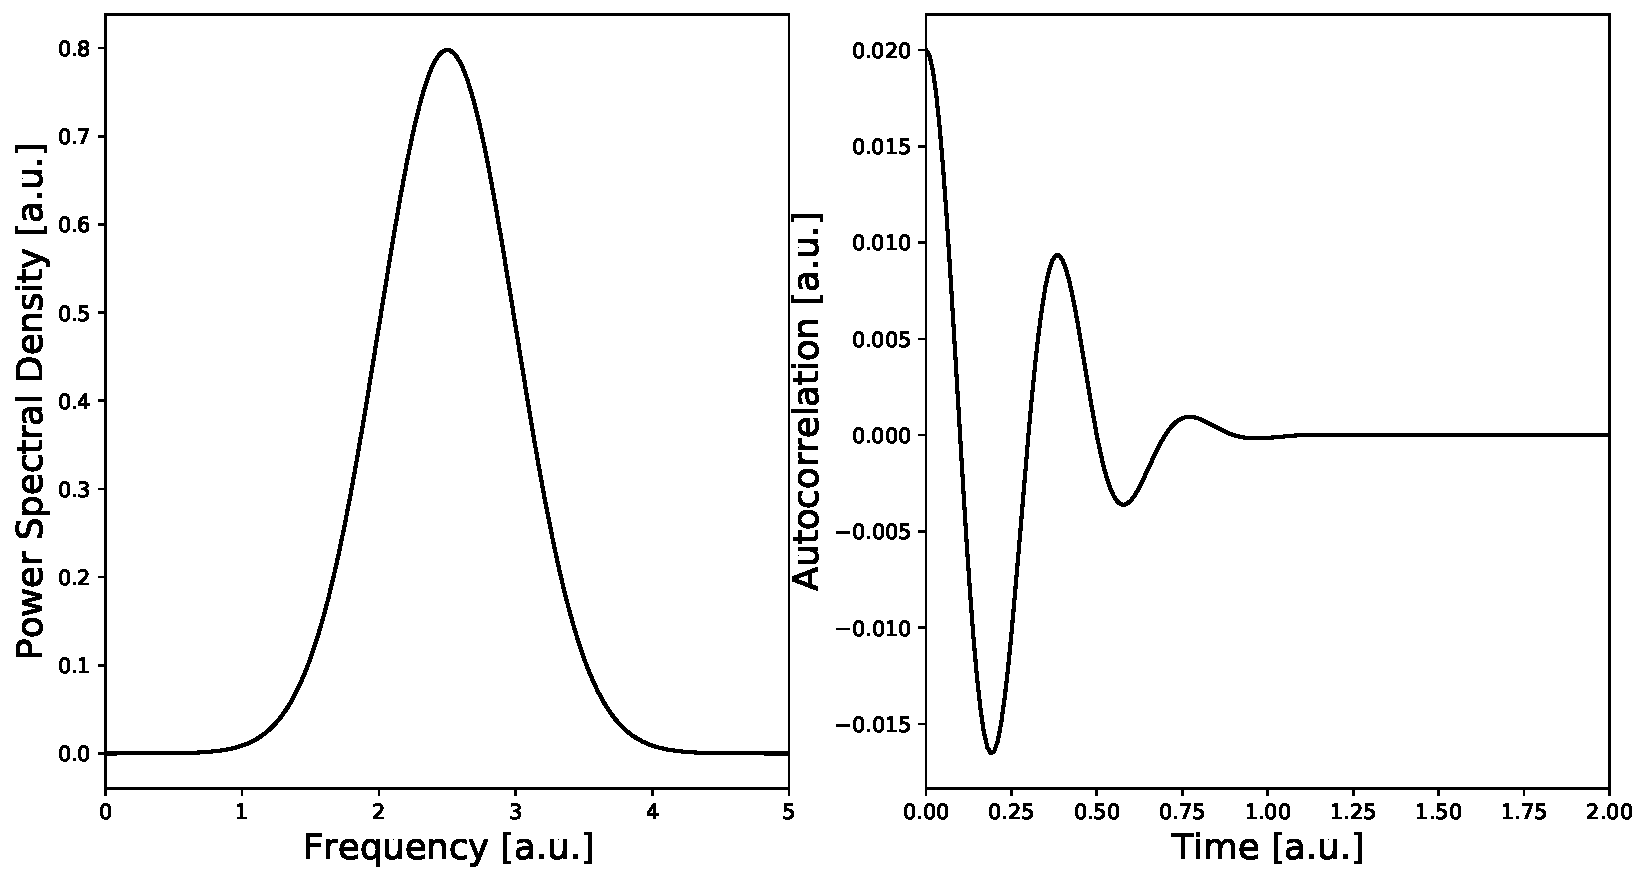
\includegraphics[width = \linewidth]{Images/Noise and PSD/NormalPSDautocorr.pdf}
	\caption{A priori spectrum (left) and autocorrelation (right)}
	\label{fig:autocorr}
\end{figure}

\begin{figure}
    \centering
        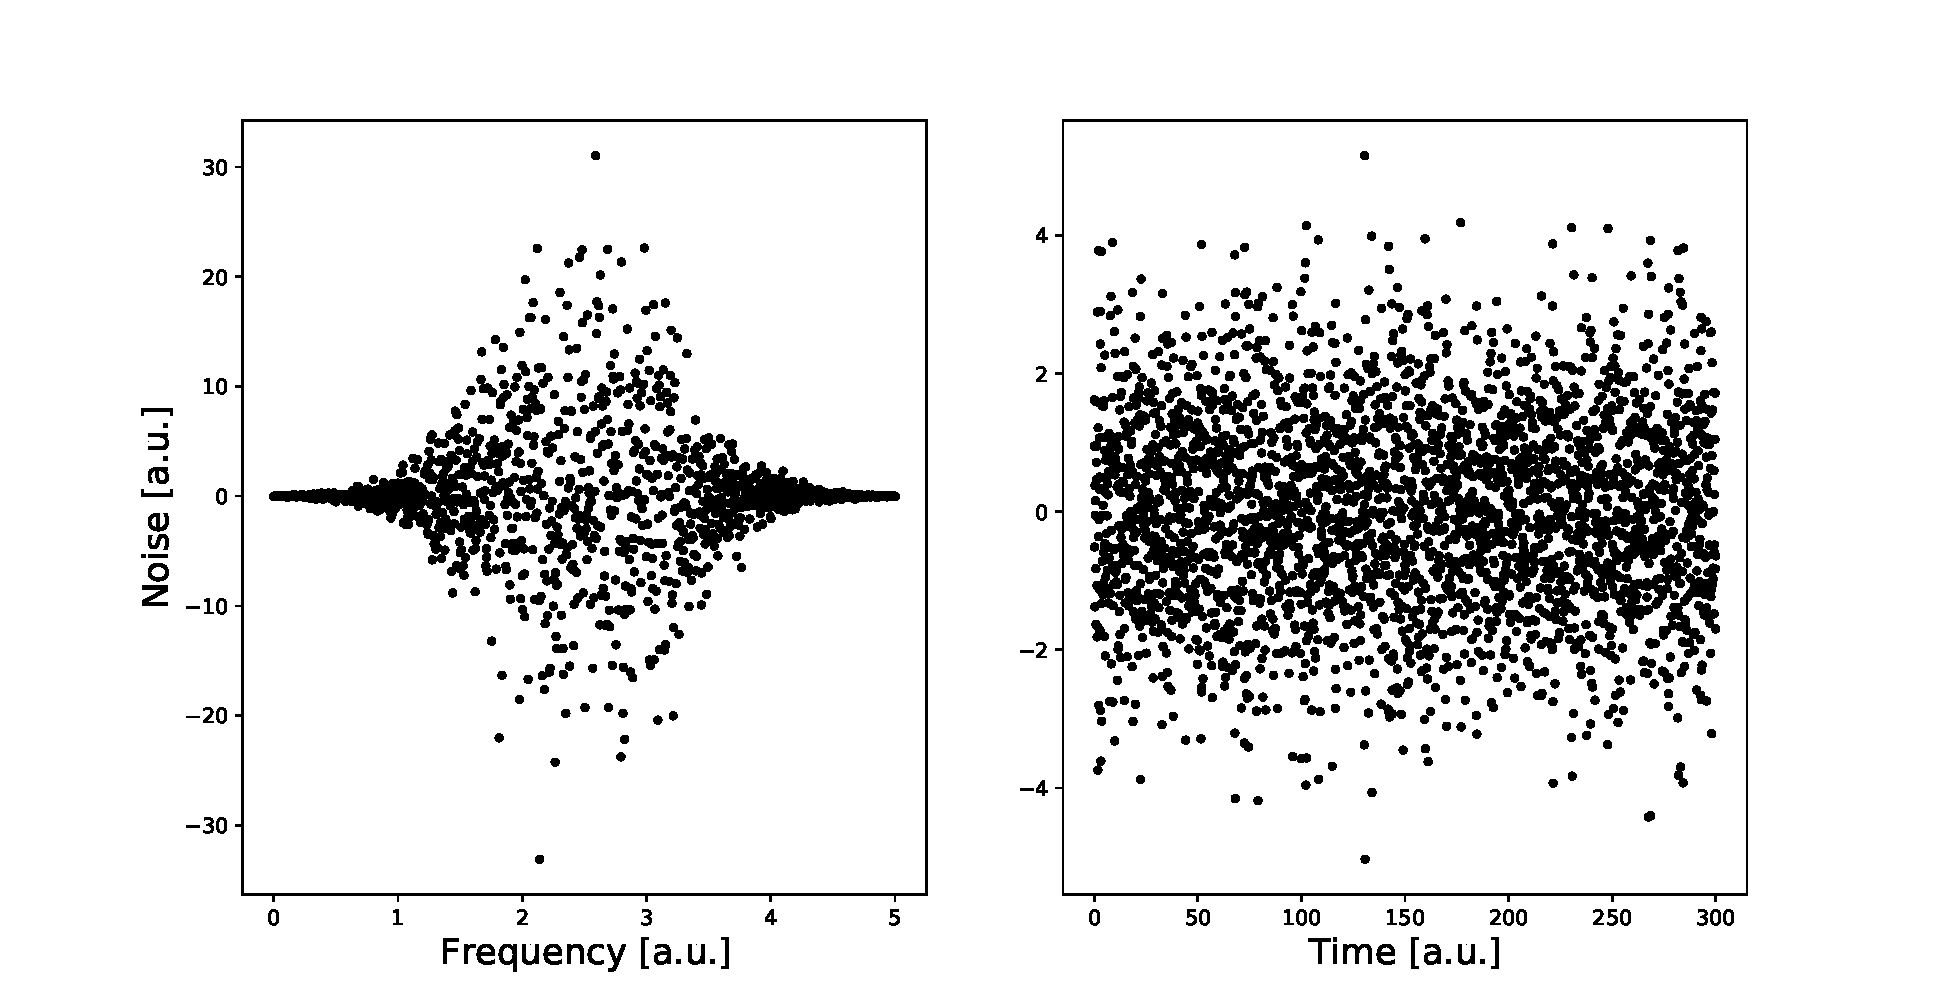
\includegraphics[width = \linewidth]{Images/NormalPSD/NormalNoise.pdf}
    \caption{Noise in both time and frequency domain. Frequency noise behaviour is representative of the chosen spectrum, having its maximum amplitude around $f = 2.5 au$}
    \label{fig:noise}
\end{figure}

For our studies, we generate a dataset of 1000 time series of 3000 points each: see fig.~\ref{fig:noise} for an example of a time series in frequency and time domain.
For every time series we will compute the spectrum with every optimization method.
To assess the magnitude of the disagreement, we compute the relative error between the mean spectrum $\hat{S}$ and the true (analytical) spectrum $S$ for every frequency bin:
\begin{equation}
r(f) = \frac{|\hat{S}(f) - S(f)|}{S(f)}\; .
\end{equation}

We report the average values of the relative error for the different optimizers in Table~\ref{tab:relative_errors}.

\sschmidt{Sono arrivato fino a qui nelle modifiche}
\begin{table}
	\caption{Average relative error for different optimizers, computed in different ways. We consider a set of $1000$ realization of a noisy time series of $3000$ points.
	We report the average error  $\bar{r}_{\bar{S}}$ on the whole set of simulations, the error $\bar{r}_{\bar S}^{\mu \pm 3\sigma} $ averaged only on data points between $3\sigma$ and the error $\bar{r}$ on a single, randomly drawn realization.
	\sschmidt{I think we need to discuss on which performance error to include in the estimation}
	}
	\label{tab:relative_errors}
	\def\arraystretch{1.5}
	\begin{ruledtabular}
		\begin{tabular}{ l c c c }
			\multirow{2}{*}{Optimizer}& \multicolumn{3}{c}{Relative Error}\\
			& $\bar{r}_{\bar{S}}$	& $\bar{r}_{\bar S}^{\mu \pm 3\sigma} $ & $\bar{r}$\\
			\hline \hline
			FPE 			& $6.9 \; (46.9\%)$	& $7 \; (1.6\%)$ & \\ 
			\hline
			CAT 			& $4.5 \; (30.6\%)$	& $194 \; (45.3\%)$ & \\
			\hline
			OBD 				& $1.7 \; (11.6\%)$	& $206 \; (48.1\%)$ & \\
		\end{tabular}
	\end{ruledtabular}
\end{table}


\begin{figure}[H]
	\centering
	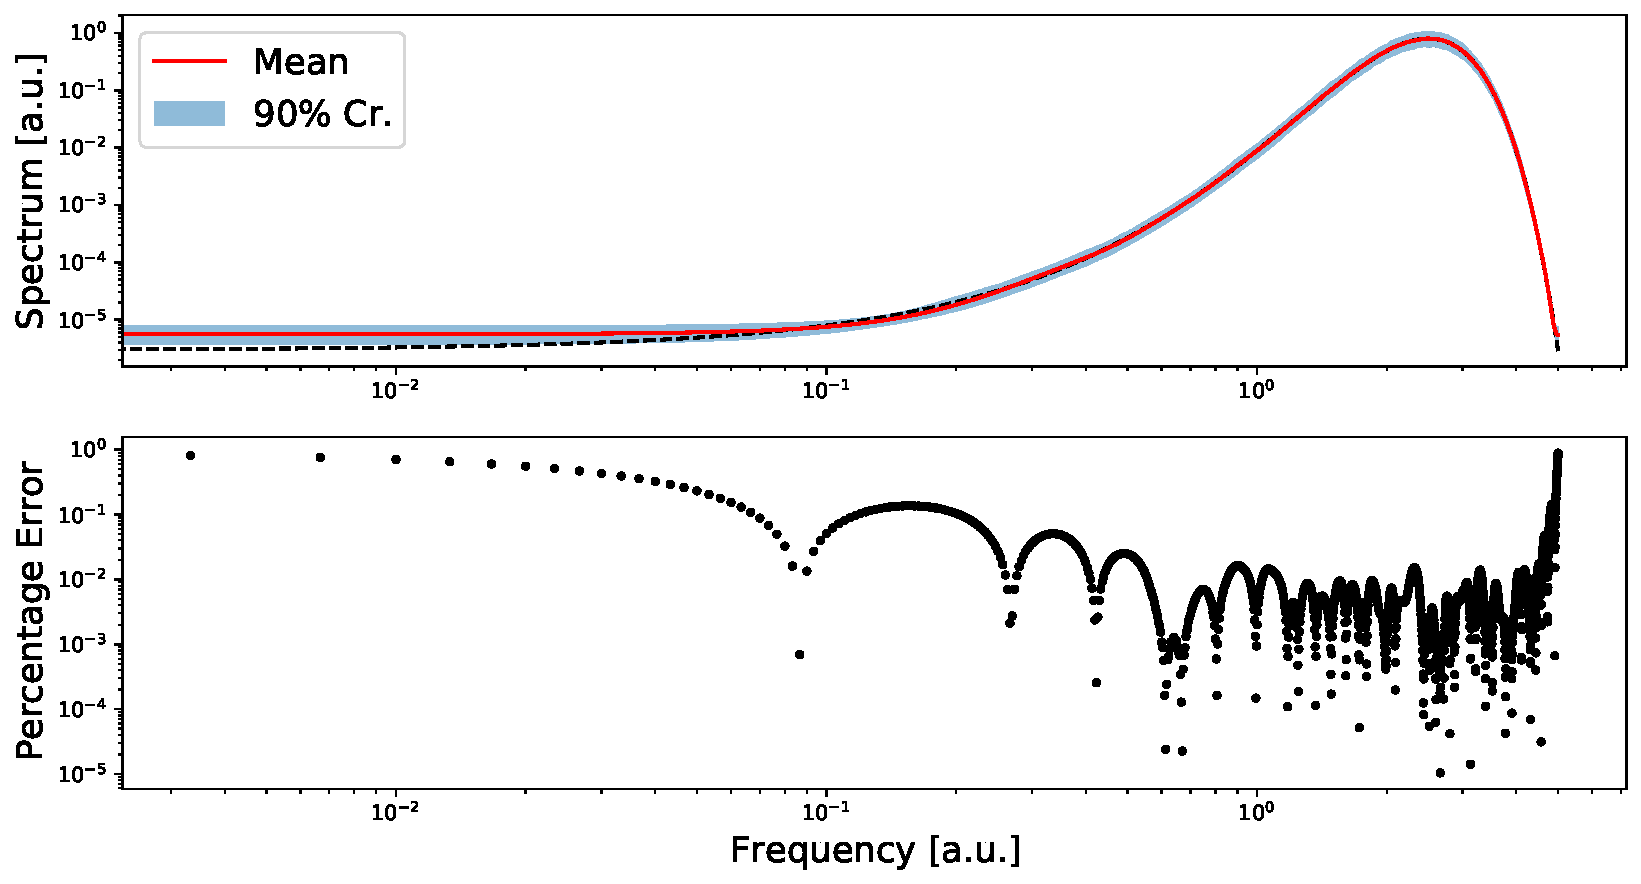
\includegraphics[width = \linewidth]{Images/NormalPSD/FPEpsdAndResiduals.pdf}
	\caption{Ensemble Average for FPE reconstruction with 90\% Credibility Regions (above) and percentage error (below)}
	\label{fig:FPEmean}
\end{figure}

\subsubsection{Final Prediction Error (FPE)}
The results of our investigation on te performance of FPE are reported in fig.~\ref{fig:FPEmean}: we plot the ``true" spectrum, the reconstructed spectrum as well as the $90\%$ credible region of the predicted spectrum.
Qualitatively, there is a good agreement between the reconstructed spectrum and the true spectrum; however, we note that the reconstruction is not very accurate in the low frequency region. 

For the entire spectrum, the mean relative error $\bar{r}$ is 
\begin{equation}  
    \bar{r}_{\bar S, FPE} = 0.025.
\end{equation}
FPE performs well in reconstructing the spectrum even with relatively short time series, with a deviation from the true spectrum around 2\%, but it is evident that it is not able to capture all the features of the spectrum, since the reconstruction in the tails is inaccurate. If we compute the average percentage error in three standard deviations from the mean we gain an order of magnitude estimate of the accuracy of the reconstruction, obtaining: 
\begin{equation}
    \nonumber
    \bar{r}_{\bar S, FPE}^{\mu \pm 3\sigma} = 0.005. 
\end{equation}
and we can state the the method is highly performant in this frequency window. 
Since it is not always possible to work with more then one realization for a process, as in observational experiments, it is important to understand how this method behaves when we apply it on a single time series. In that case, the mean error and its standard deviation are: 
\begin{equation}
    \nonumber
    \bar r_{FPE} = 0.16; \quad \sigma_{r} = 0.16\,.
\end{equation}
The average error of a reconstruction based on a single time series is bigger than the one obtained considering the average of all the reconstructions.
Standard deviation of the errors assume small values and 90\% credibility regions (Cr.) in \ref{fig:FPEmean} are tight. This means that if we randomly take two of the reconstructed spectra, we expect their differences to be statistically small. These facts are evidence for FPE to be a relatively stable optimizer. 
We already said that the estimate for filter's length lays in a well defined range of values. The quality of the reconstruction, as noted in Chapter 1, depends on the order of the reconstructed AR process. 
To investigate this idea further, we plot the value of the optimizer for each recursion and the residuals as a function of the estimate for the order of the autoregressive process (\textbf{Figure \ref{fig:FPEErrorOrder}}),

\begin{figure}[H]
    \noindent
    \centering
    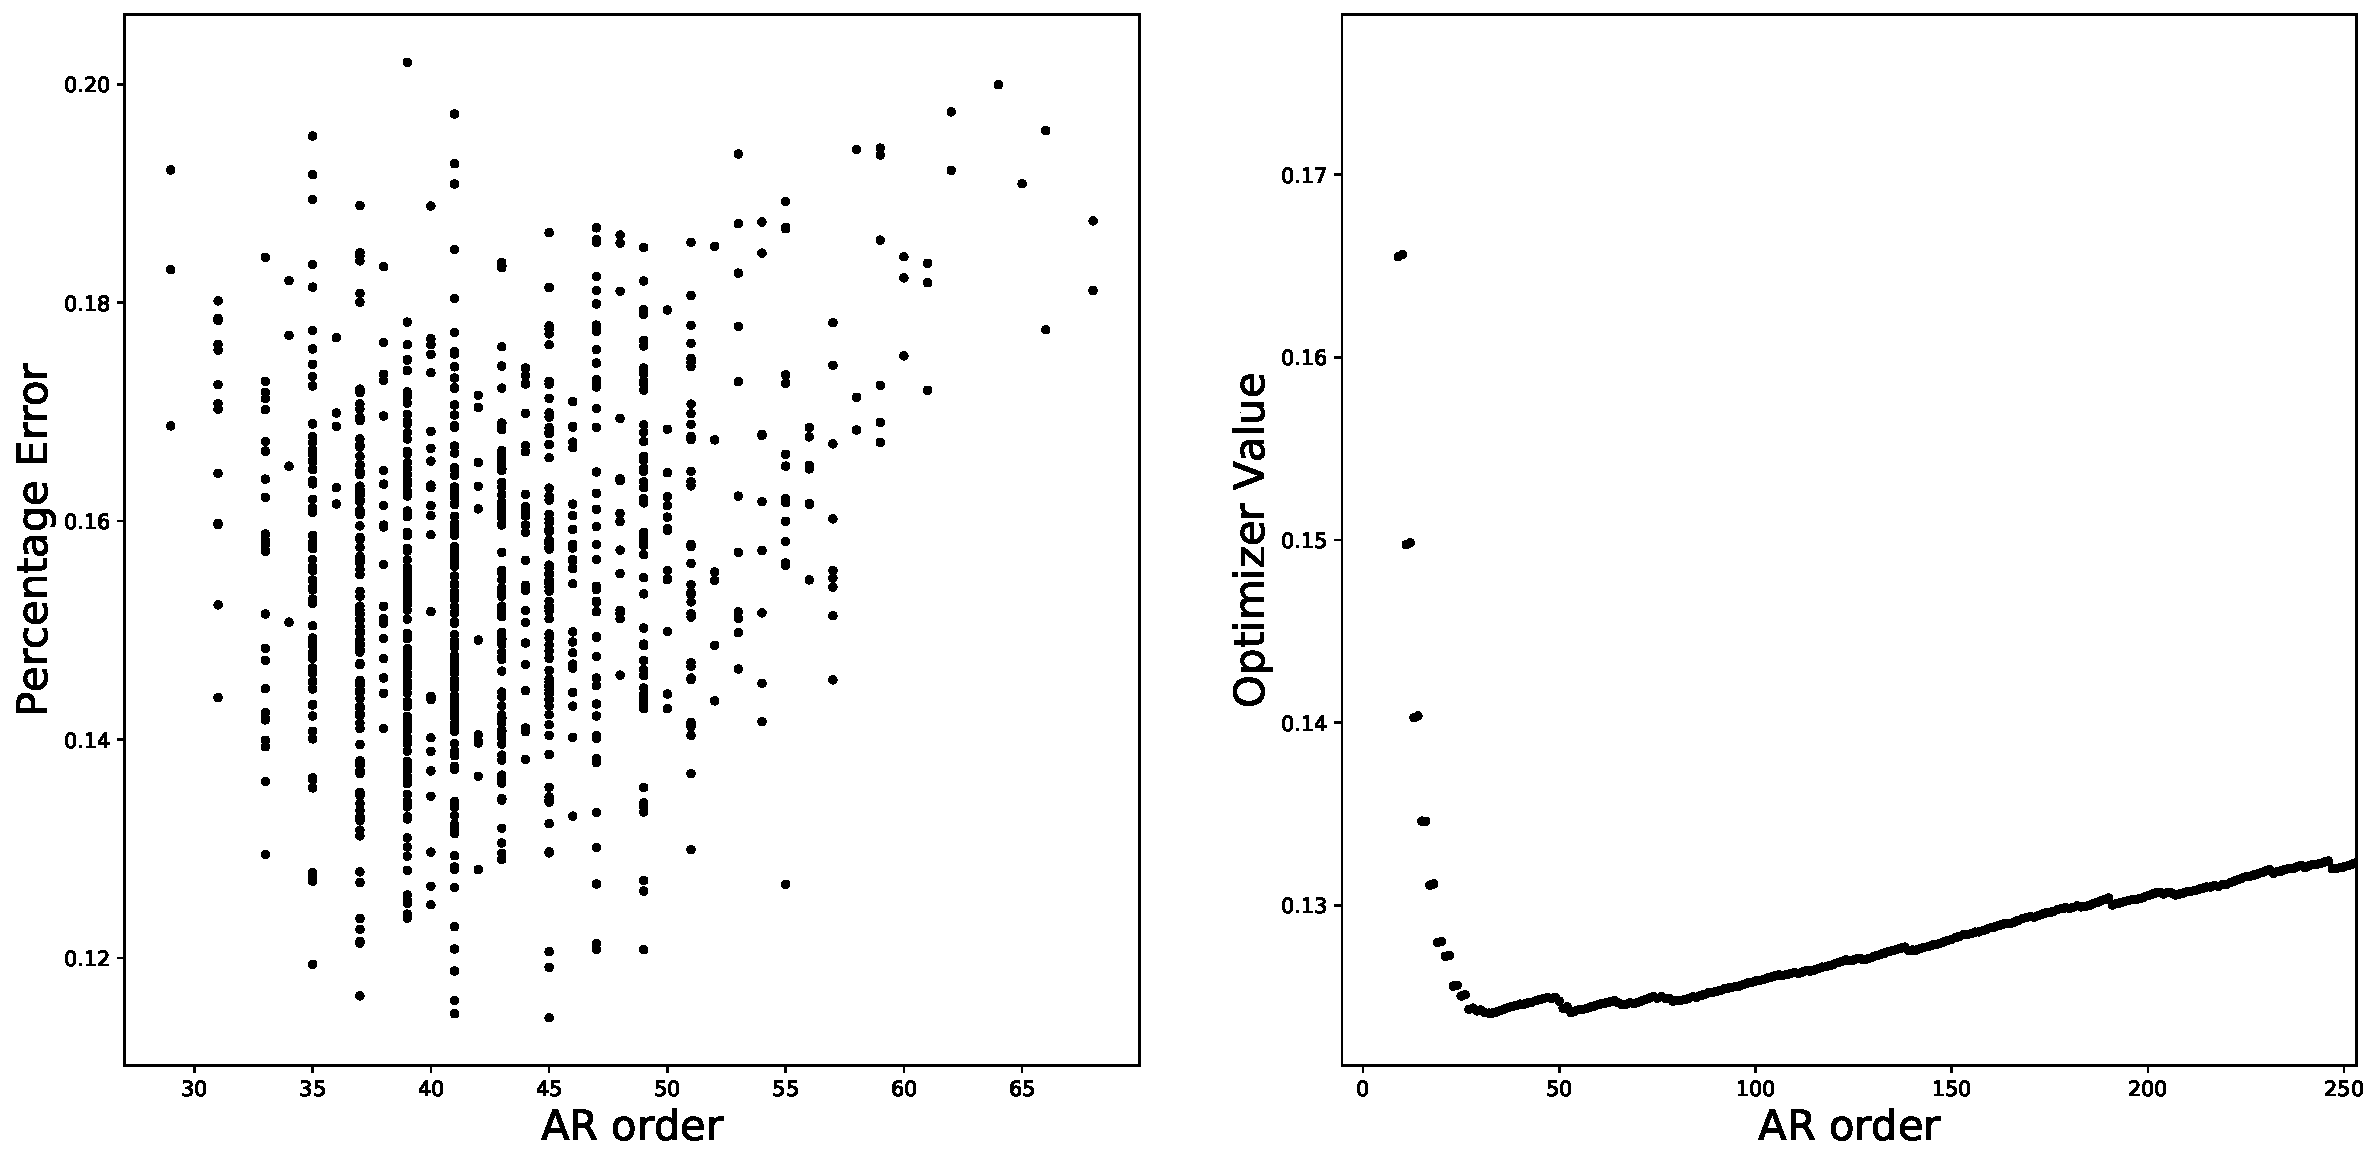
\includegraphics[width = \linewidth]{Images/NormalPSD/FPEoptimizer.pdf}
    \caption{Stability of FPE, that results in a cluster of values in a small region (left), is due to the typical behaviour of the optimizer as a function of the AR order (right).}
    \label{fig:FPEErrorOrder}
\end{figure}
Foremost evidence for the stability of this optimizer is found in its values as a function of the AR order. Figure \ref{fig:FPEErrorOrder} shows that Values tend to decrease monotonically until a sharp and well defined minimum is reached, to start growing again after this area. This is representative of the typical behaviour of this optimizer as a function of the length of the filter, and explains why the estimates for AR orders are confined in a small region. This plot also shows that most of the values collapsed in the region of AR orders comprised between 30 an 50. There are only few values outside this interval, and get fewer as order's estimate increases. In this region, there is no strong evidence of some correlation between the estimate for M and its associated relative error. It is important to notice that the estimate associated with the higher values of M (around $M > 60$) exhibit the highest 'mean' relative error. \\ 
We conclude that the FPE shows good quality reconstruction for the spectrum and very desirable stability properties, its estimate for filter's length M is clustered in a region where there is no dependence of error from M. 
\subsubsection{Optimum Bayes Decision Rule (OBD)}
The second optimizer in consideration is OBD.  (\textbf{Figure \ref{fig:OBD3000}}) shows a good agreement between the average over the reconstructions and true spectrum.
\begin{figure}[H]
    \centering
    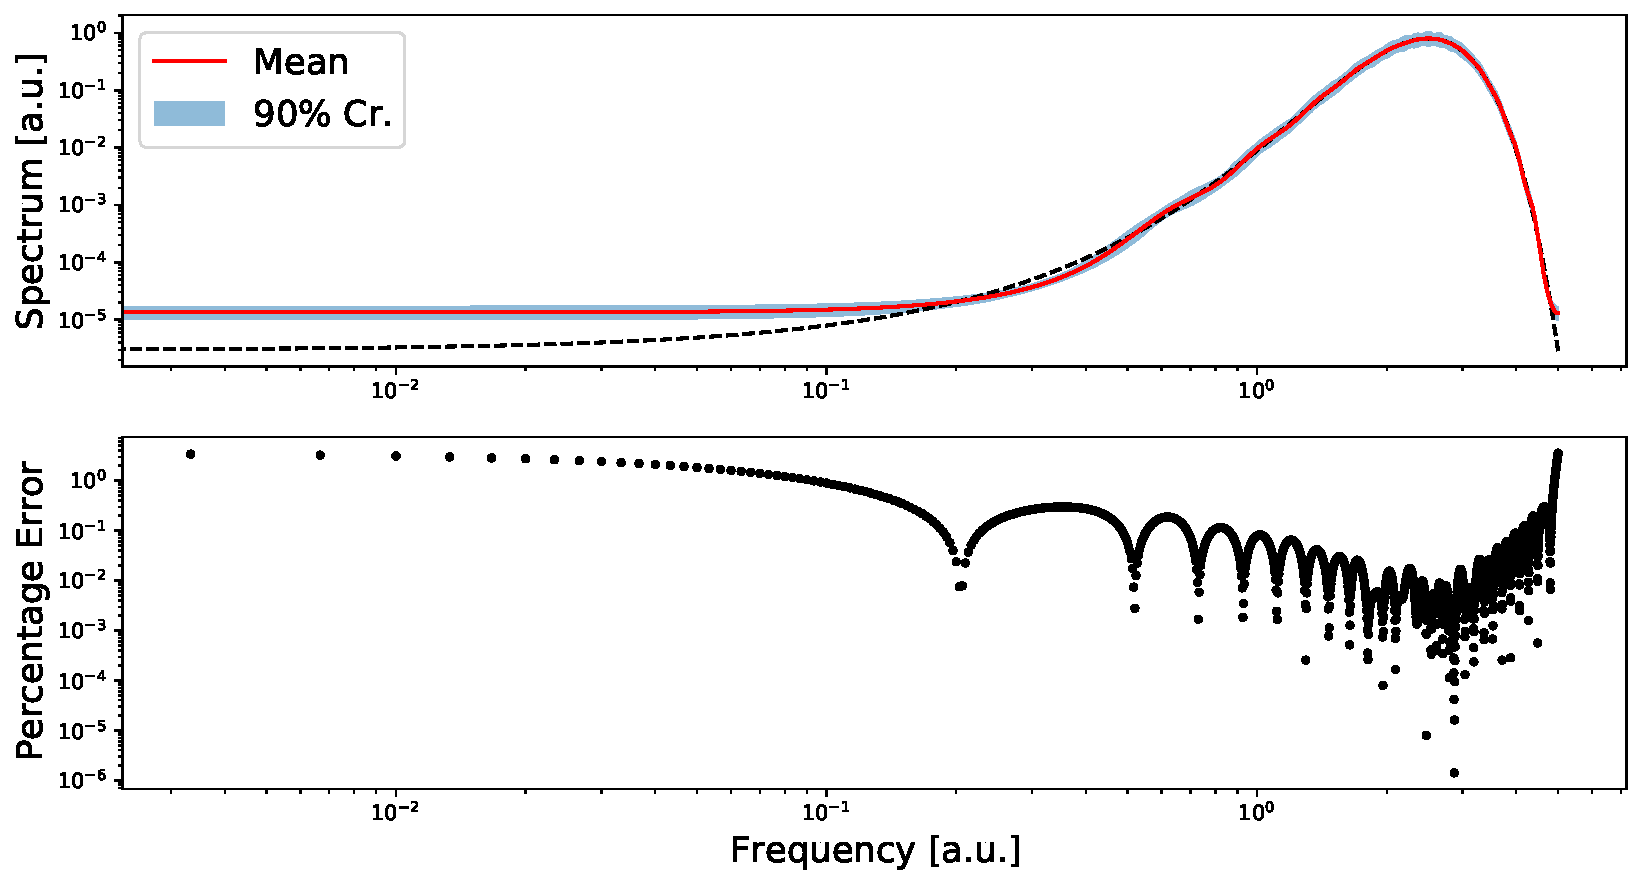
\includegraphics[width = \linewidth]{Images/NormalPSD/OBDpsdAndResiduals.pdf}
    \caption{Reconstruction of the spectrum from 1000 simulations with OBD optimizer. Plot is mean of all the results with 90\% credibility regions (above) and percentage error (below)}
    \label{fig:OBD3000}
\end{figure}
The same behaviour of FPE is observed, a good quality reconstruction at the center of the distribution with quite small Credibility regions (Cr.) at a $90$\% credibility level.
Qualitatively they behave similarly but quantitatively the disagreement of this method is found to be even larger than the one obtained with FPE, as can be noticed in the plot of relative errors in figure \ref{fig:OBD3000} (below) where at the extremes the inaccuracy is even larger than 300\% with respect to the real value of the spectrum. For the overall spectrum and within three standard deviation from the mean, we find that the reconstructed spectrum has a deviation of
\begin{equation}
    \nonumber
    r_{\bar S, OBD} = 0.15, \qquad r^{\mu \pm 3\sigma}_{\bar S, OBD} = 0.018. 
\end{equation}
When applied to single realizations of the time series, we find
\begin{equation}
    \nonumber
    \bar{r}_{OBD} = 0.237, \qquad \sigma_{r, OBD} = 0.0296.
\end{equation}
It is interesting to notice that overall relative error of the average spectrum is of the same order of magnitude of the average single reconstruction for the spectrum. Averaging over a 1000 realisations does not substantially improve our results. As a function of the filter length, the values taken by the OBD cluster in a small region, indicating the stability of the reconstructed process order $M$.

\begin{figure}[H]
    \centering
    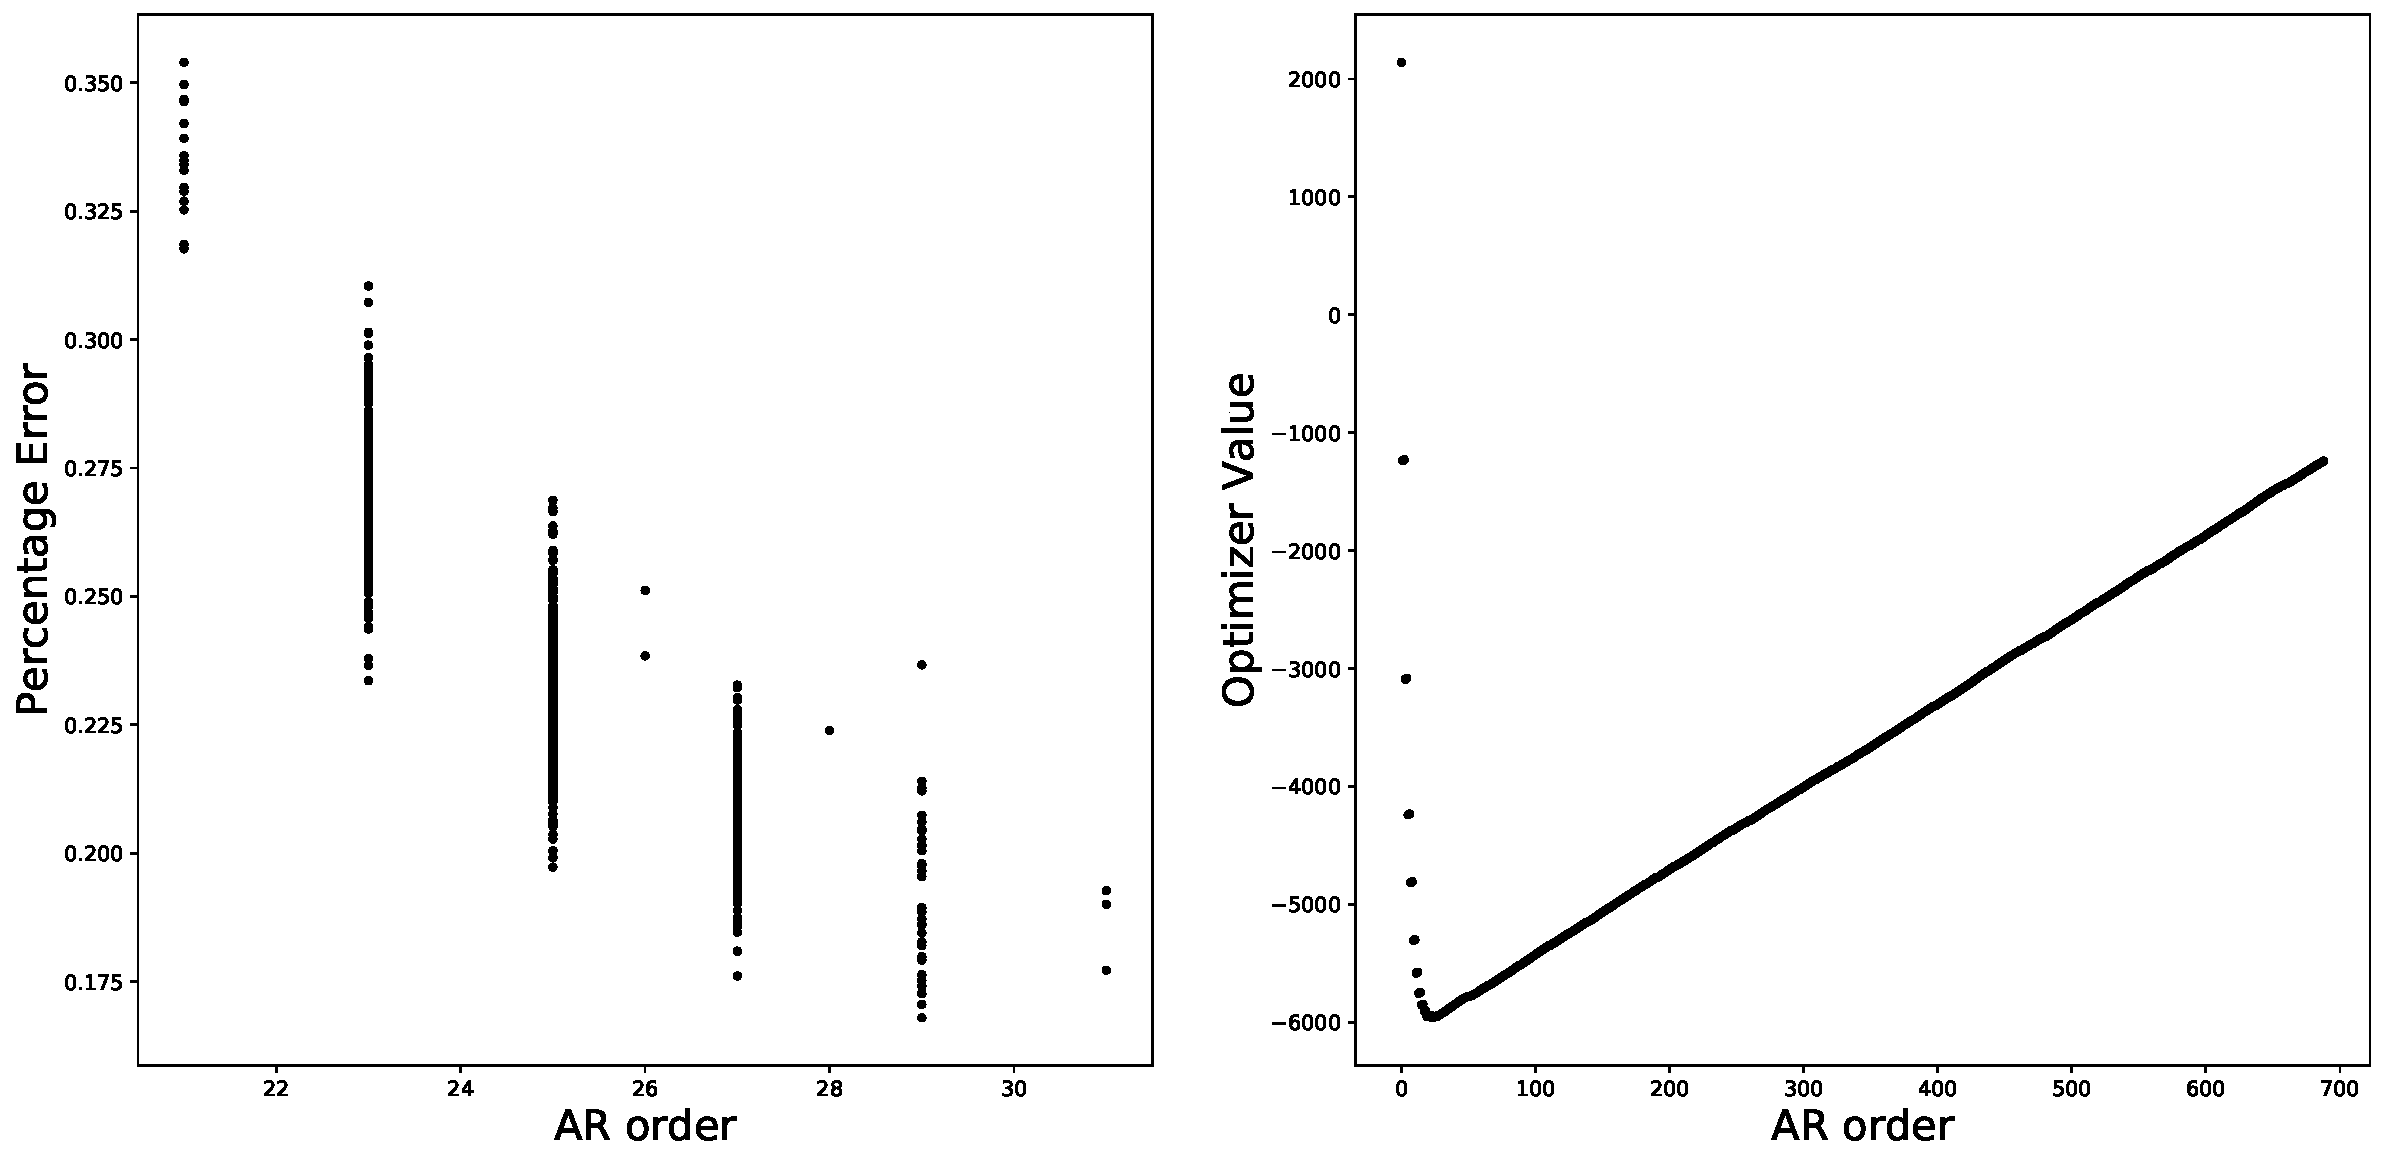
\includegraphics[width = \linewidth]{Images/NormalPSD/OBDoptimizer.pdf}
    \caption{Stability of OBD, that results in a cluster of values in a small region (left), is due to the typical behaviour of the optimizer as a function of the AR order (right)}
       \label{fig:OBDErrorOrder}
\end{figure}we see that again our results are clustered in a very small region, due to the behaviour of the optimizer that converge in a small area before growing again. The estimate of the length of the filter is around $p = 20 \div 30$.Note the difference compared to FPE (see \ref{fig:FPEErrorOrder}); for OBD the mean relative error depends on $M$ as
\begin{equation}
    \hat r \sim M ^ {-2.016 \pm 0.006}.
\end{equation}
In summary, OBD shows greater error wherever in the spectrum, due to the fact that it choose filters that are too short and in a region where quality drastically change when changing M. In this case we can say that we have a stable estimate for M, but due to this dependence, the estimate is not as stable as FPE's. 
\subsubsection{Criterion Autoregressive Transfer function (CAT)}
This last criterion differs substantially from the two other optimizers. Figure \ref{fig:CATmean} (above) shows a good agreement between the estimate of the spectrum for every frequency
\begin{figure}[H]
    \centering
    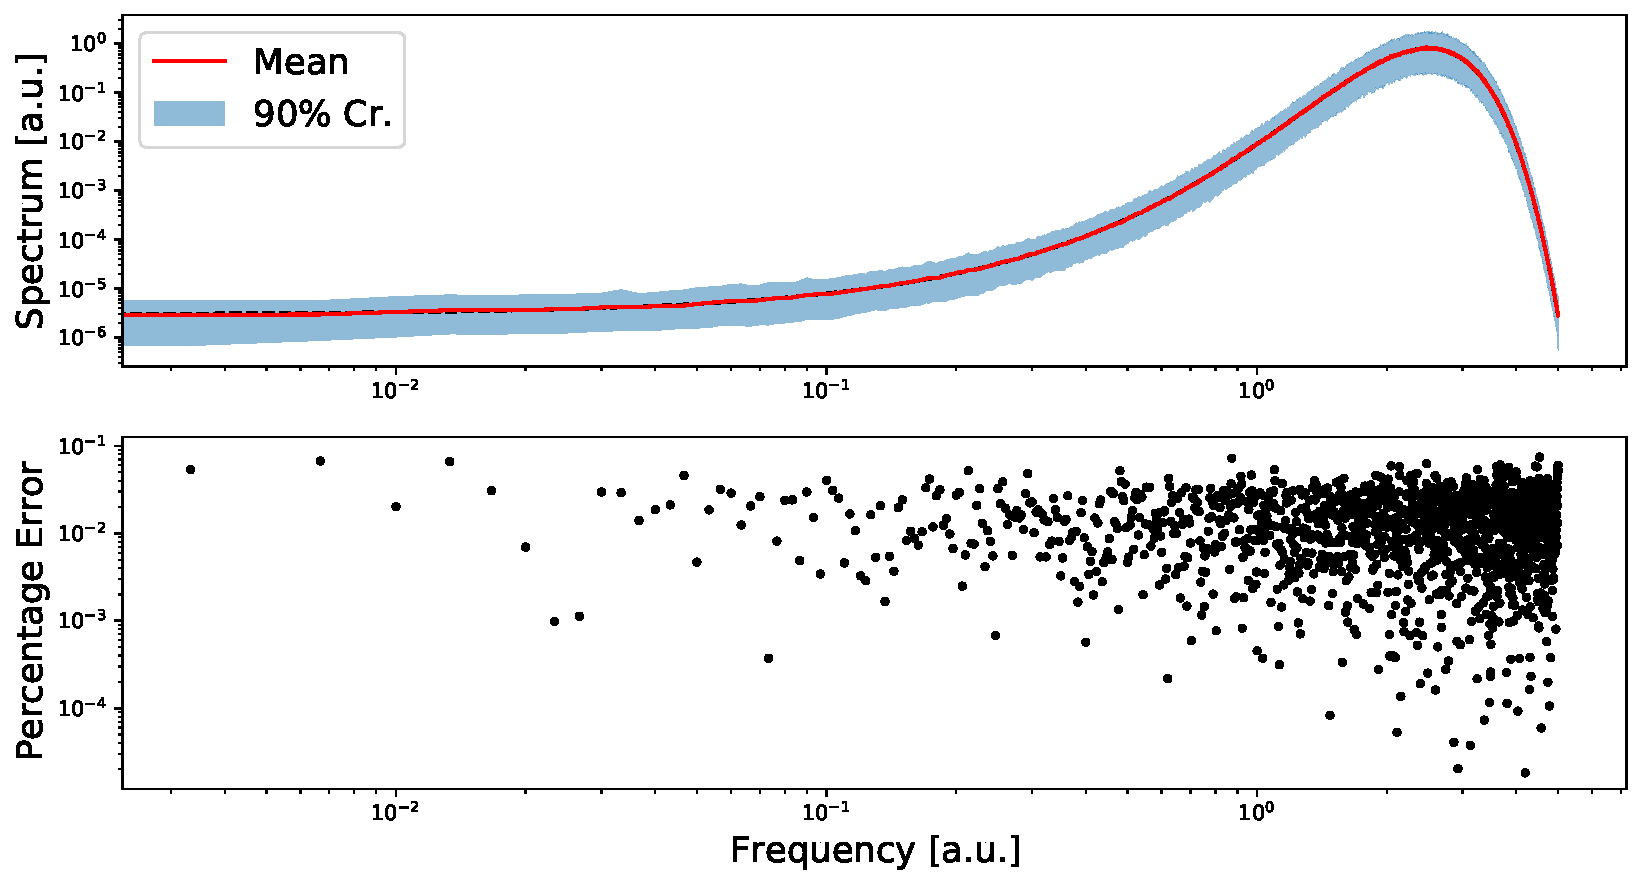
\includegraphics[width = \linewidth]{Images/CAT/CATnormal.pdf}
    \caption{Mean spectrum for CAT optimizer, 1000 simulations for 3000 points datasets}
    \label{fig:CATmean}
\end{figure} and also tails are well captured by the average spectrum. However, the variance of the reconstructed spectrum is quite large, much larger than for FPE and OBD. In general, the relative error is nearly constant, $\sim 10\%$ over all frequencies, see  Fig. \ref{fig:CATmean} (below). The residuals, averaged over all frequencies, are: 
\begin{equation}
    \nonumber
    \bar r_{\bar S, CAT} = 0.016 \qquad \bar r^{\mu \pm \sigma}_{\bar S, CAT} = 0.017.
\end{equation}
the overall reconstruction is thus quite accurate, with deviations from the simulated spectrum of the order of $1\% \div 2\%$.\\
The picture drastically changes in the case of individual time series realizations. The average residuals are, in fact
\begin{equation}
    \bar r_{CAT} = 0.42 \qquad \sigma_{CAT} = .44\,.
\end{equation}
The error is indeed $\sim 42\%$, hence much larger than in the case of FPE and OBD. Both large error bars and the large standard deviation are indications of the instability of this optimizer. This is exemplified by the variety of different spectra that can be obtained considering different time series. 

\begin{figure}[H]
    \centering
    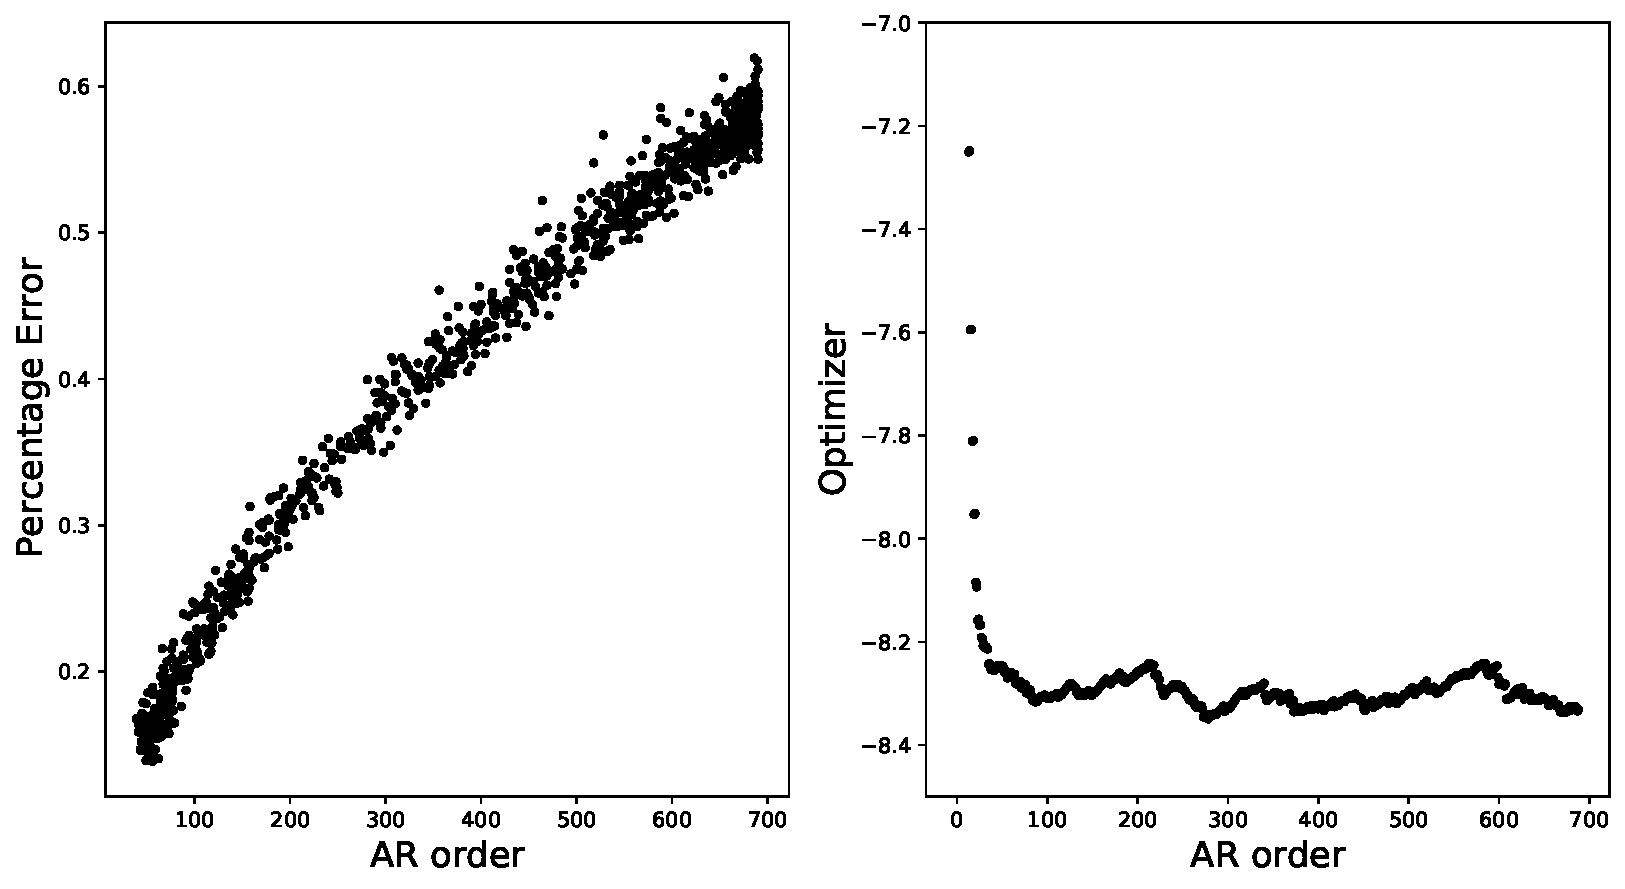
\includegraphics[width = \linewidth]{Images/CAT/CAToptimizer1.pdf}
    \caption{CAT is not a stable optimizer since its optimizer do not converge to any specific region of the AR estimate order}
    \label{fig:CAToptimizer}

\end{figure}
The reason for this behaviour, can be found in \textbf{Figure (\ref{fig:CAToptimizer})}. CAT does not converge to any specific value for the order of the autoregressive process. In turn, this results in estimates for the order that span a large range.  Figure \ref{fig:CAToptimizer} also shows a strong dependence of the error on the estimated length of the filter. The good quality of the reconstruction from the average spectrum can be explained as follows: long filters are able to capture features that short filters cannot see, like the big excursion in the size of datas of a normal distribution, but this length is also responsible of an augmented variance in the estimate, introducing spurious peaks in the reproduction (Figure \ref{fig:GaussMedian})

Averaging, the noise in each spectrum is cancelled. It is interesting that the cancelling of errors in averaging is property of gaussian noise (the process is gaussian, after all). This implies, in a sense, that each estimate of the spectrum is independent of any other, as suggested by the huge variance in the residuals. This instability is not a good property for an estimation, so that this estimator might be found to be optimal for repeatable experiments and not for single observation of some process. Another approach to this method will be proposed in section \ref{sec:ACAT}

\begin{figure}
    \centering
    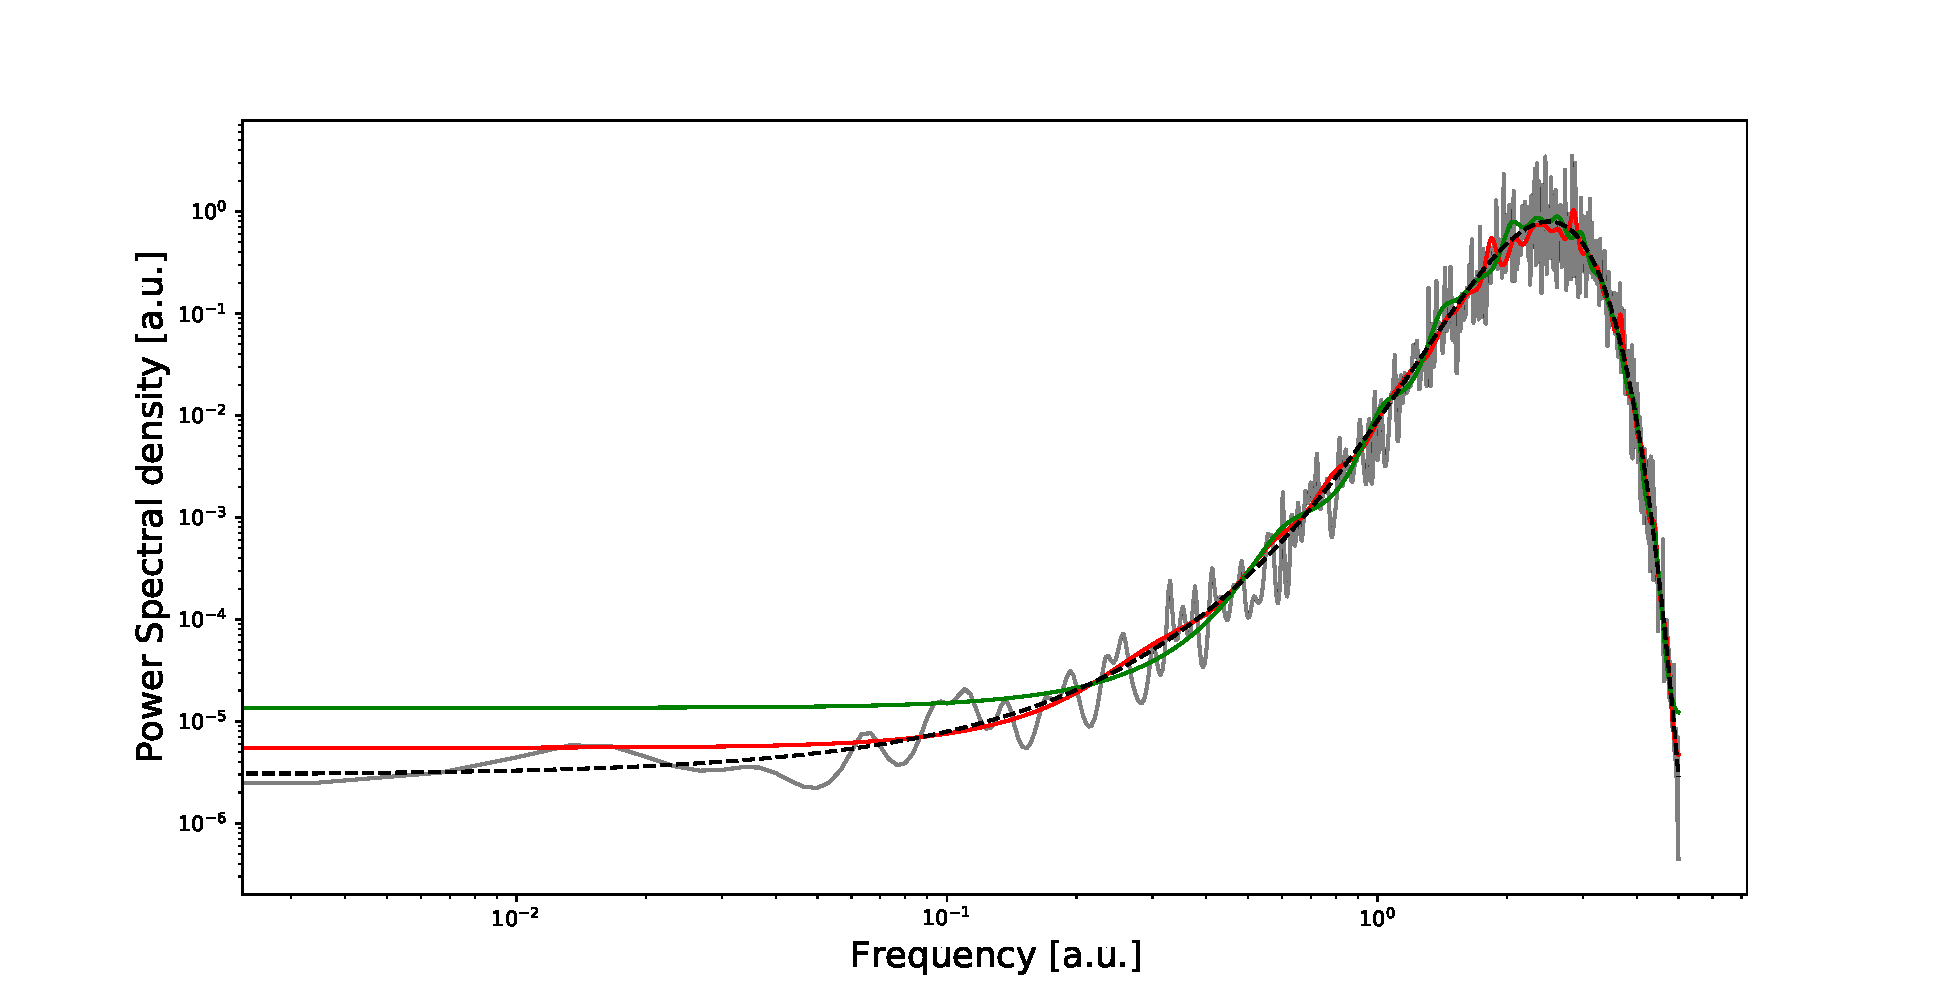
\includegraphics[width = \linewidth]{Images/NormalPSD/Gaussmedian.pdf}
    \caption{Reconstructed power spectral density with the three method. The reported reconstruction is the one that shows the median percentage error (overall)}
    \label{fig:GaussMedian}
\end{figure}
\subsubsection{Conclusive Remarks}
\begin{figure}
    \centering
    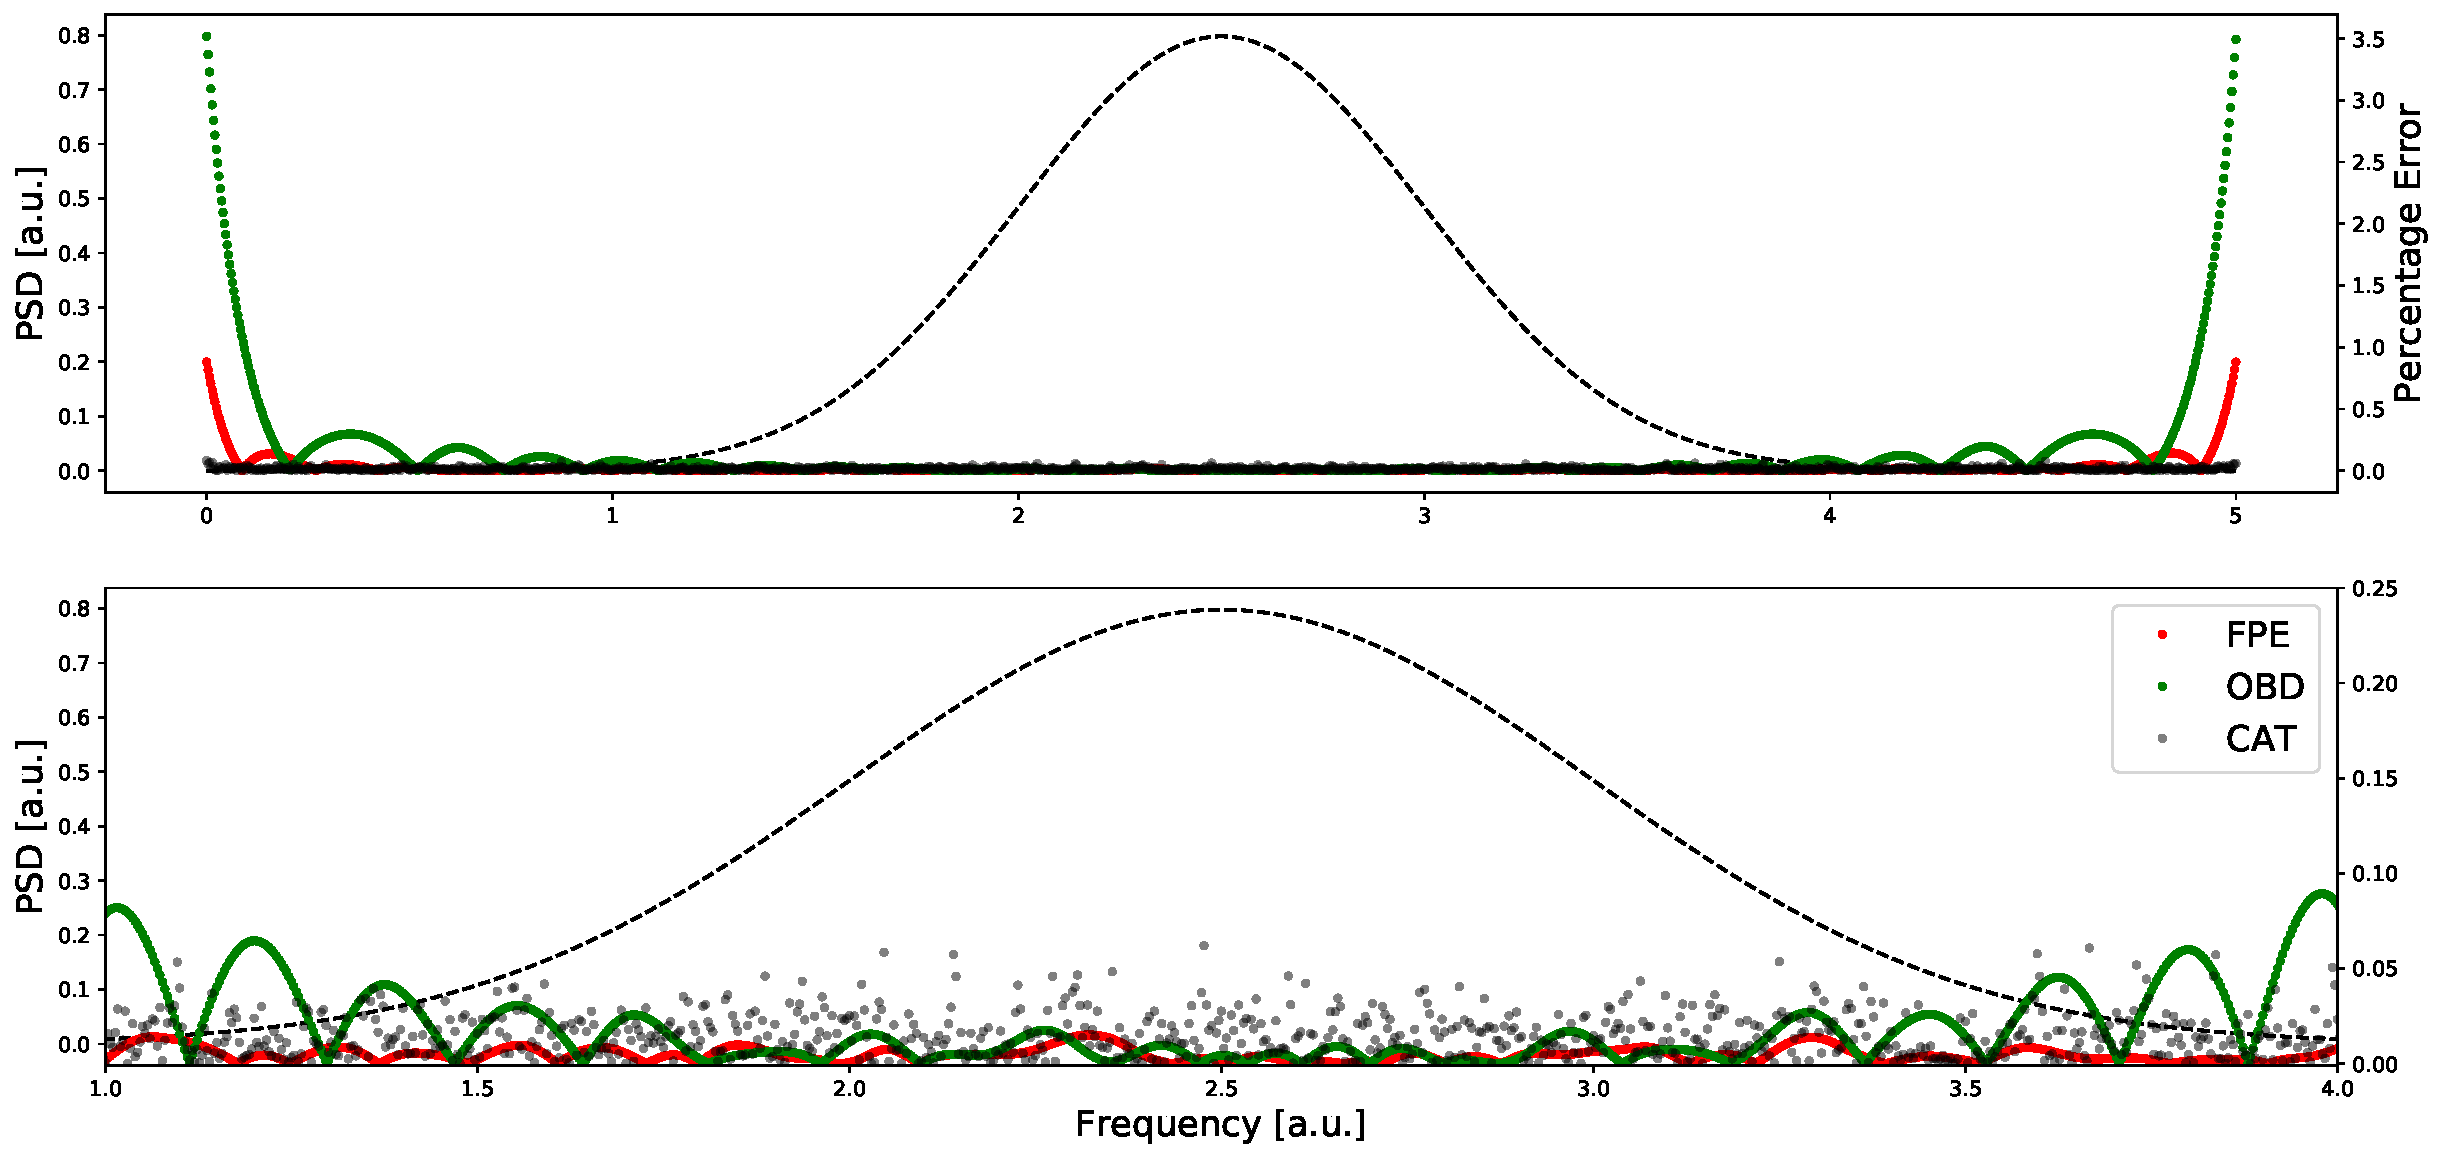
\includegraphics[width = \linewidth]{Images/NormalPSD/Normal Residuals.pdf}
    \caption{Percentage error in the reconstruction for every optimizer, as a function of the frequency. Lower panel restricts the domain to three standard deviation to increase the definition}
    \label{fig:NormalEnsembleResiduals}
\end{figure}
In our analysis, FPE and OBD optimizers are found to behave similarly while CAT shows completely different properties. Studying the average spectrum is not sufficient to choose which method behaves better. \\ 
The bad behaviour in the reconstruction of the tails from OBD and FPE might be due to the fact that very small values require longer filters. 
In fact when we consider the average for all the spectra we note that the shorter the filter the larger the error in the tails: OBD, which select the shortest filters, arrives to a $300 \%$ error at the extrema of the power spectral density, FPE which select intermediate order has got a $85\%$ error in same window, while CAT, that selects a wide range of long filters, has got a constant accuracy everywhere in the spectrum.  \\ 
Figure \ref{fig:NormalEnsembleResiduals} shows that CAT is the method that minimizes errors in the tails (upper plot), but if one restrict to three standard deviations from the mean, FPE is found to reach best accuracy (lower plot). 
The frequency averaged percentage error is reflecting this behaviour. Considering the whole reproduction, error's average and standard deviation are found to be: 
\begin{align*}
\centering
&r_{\bar S, FPE} = 0.025; \quad \sigma_{\bar S, FPE} = 0.083;  \\
&r_{\bar S, OBD} = 0.15;\quad \sigma_{\bar S, OBD} = 0.42 ; \\ 
&r_{\bar S, CAT} = 0.015; \quad \sigma_{\bar S, CAT} = 0.012
\end{align*}
In is interesting to see that the average for FPE and OBD is strongly affected from the high value of the error in the tails of the distribution. If one consider the three standard deviations from the mean, the value of the error substantially decreases, 
\begin{align*}
\centering
&r_{\bar S, FPE} = 0.005; \quad \sigma_{\bar S, FPE} = 0.004;  \\
&r_{\bar S, OBD} = 0.018;\quad \sigma_{\bar S, OBD} = 0.019 ; \\ 
&r_{\bar S, CAT} = 0.015; \quad \sigma_{\bar S, CAT} = 0.011
\end{align*}
showing that the overall percentage error is just a first indicator for the quality of the reproduction, but is not sufficient to perform a full characterization. \\
It is evident that tails do not affect CAT  average error and standard deviation at all, so that it's accuracy is approximately constant everywhere in the spectrum. \\ \ 
Since both FPE and CAT shows pros and cons, at this level, there is no reason to choose between them.\\ 
Analyzing the resolution of the single reconstruction, figure \ref{fig:optcomparison} clearly shows that FPE minimize overall relative error giving a stable result.\\ 
CAT instead shows a larger error and do not converge to any specific value. Almost every reproduction obtained with CAT is worst with respect to those obtained with FPE, but their mean is more precise. \\ 
It's instability is probably the cause for this behaviour. Since it does not show a strong convergence to some order with respect to others, very different lengths are selected.
Longer lengths are able to capture a lot of details but are more likely to introduce noise. In other words, long filters reduce bias but increment the variance of the result. 
Taking the average, for central limit theorem the error decreases as $\sim \frac{1}{\sqrt{N}}$. In this way we compensate noise and obtain a spectrum with small bias and small fluctuations.
Considering the average, CAT reconstruct precisely and with good accuracy every part of the spectrum, even if in "regular" parts best accuracy is reached from FPE. For a single reproduction, CAT is very noisy and unstable, while FPE performs the better. \ref{fig:optcomparison}
\begin{figure}
    \centering
    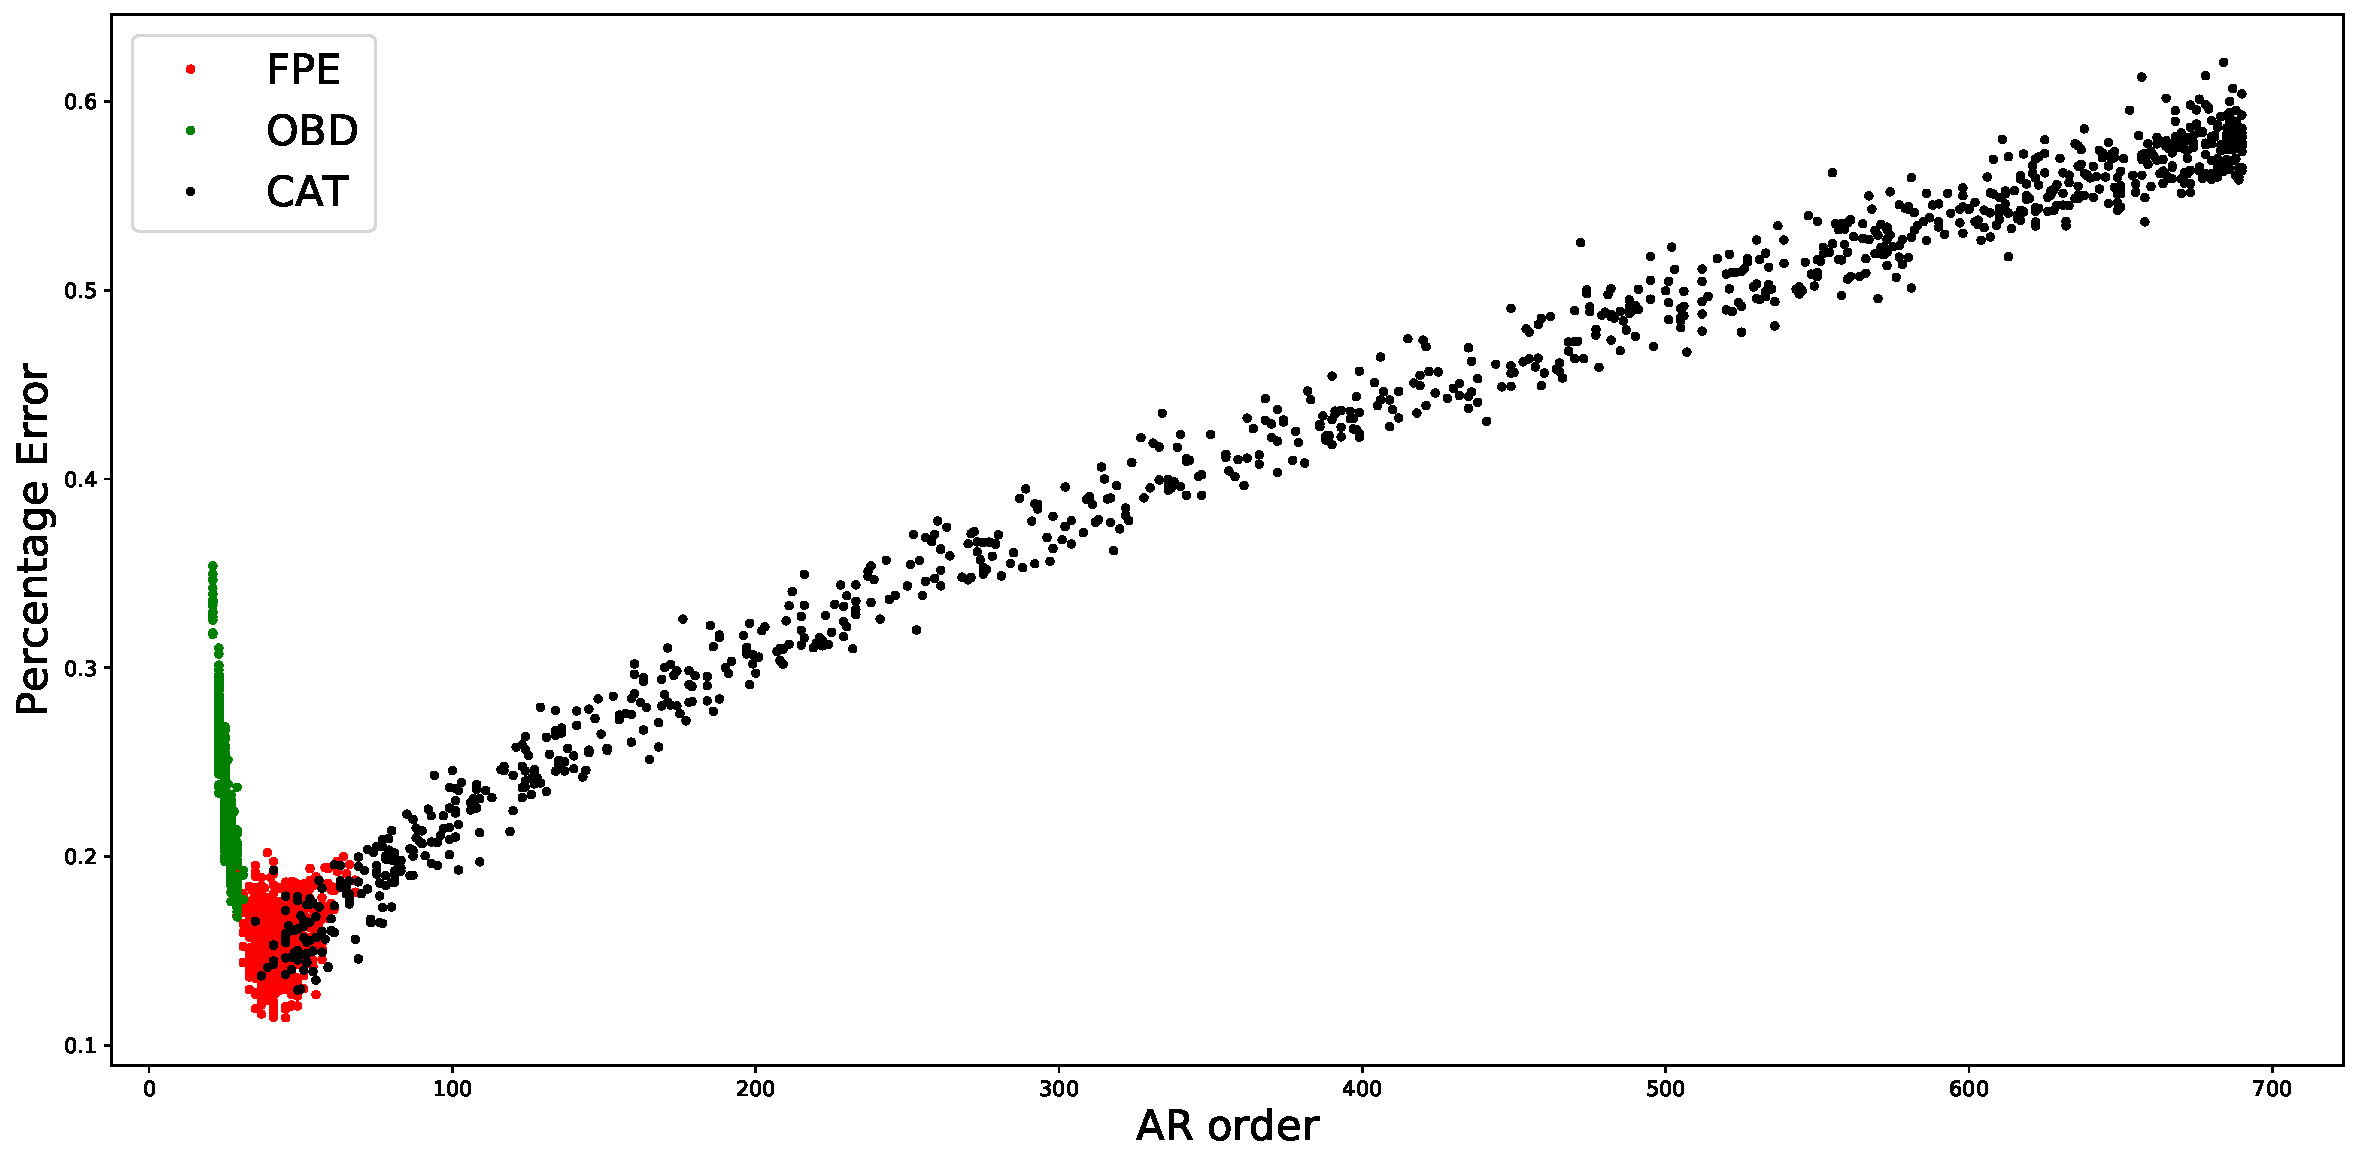
\includegraphics[width = \linewidth]{Images/NormalPSD/NormalPSDcomparison.pdf}
    \caption{Relative error as function of the length of the filter.}
    \label{fig:optcomparison}
\end{figure}
\begin{figure}
    \hfill
    \centering
    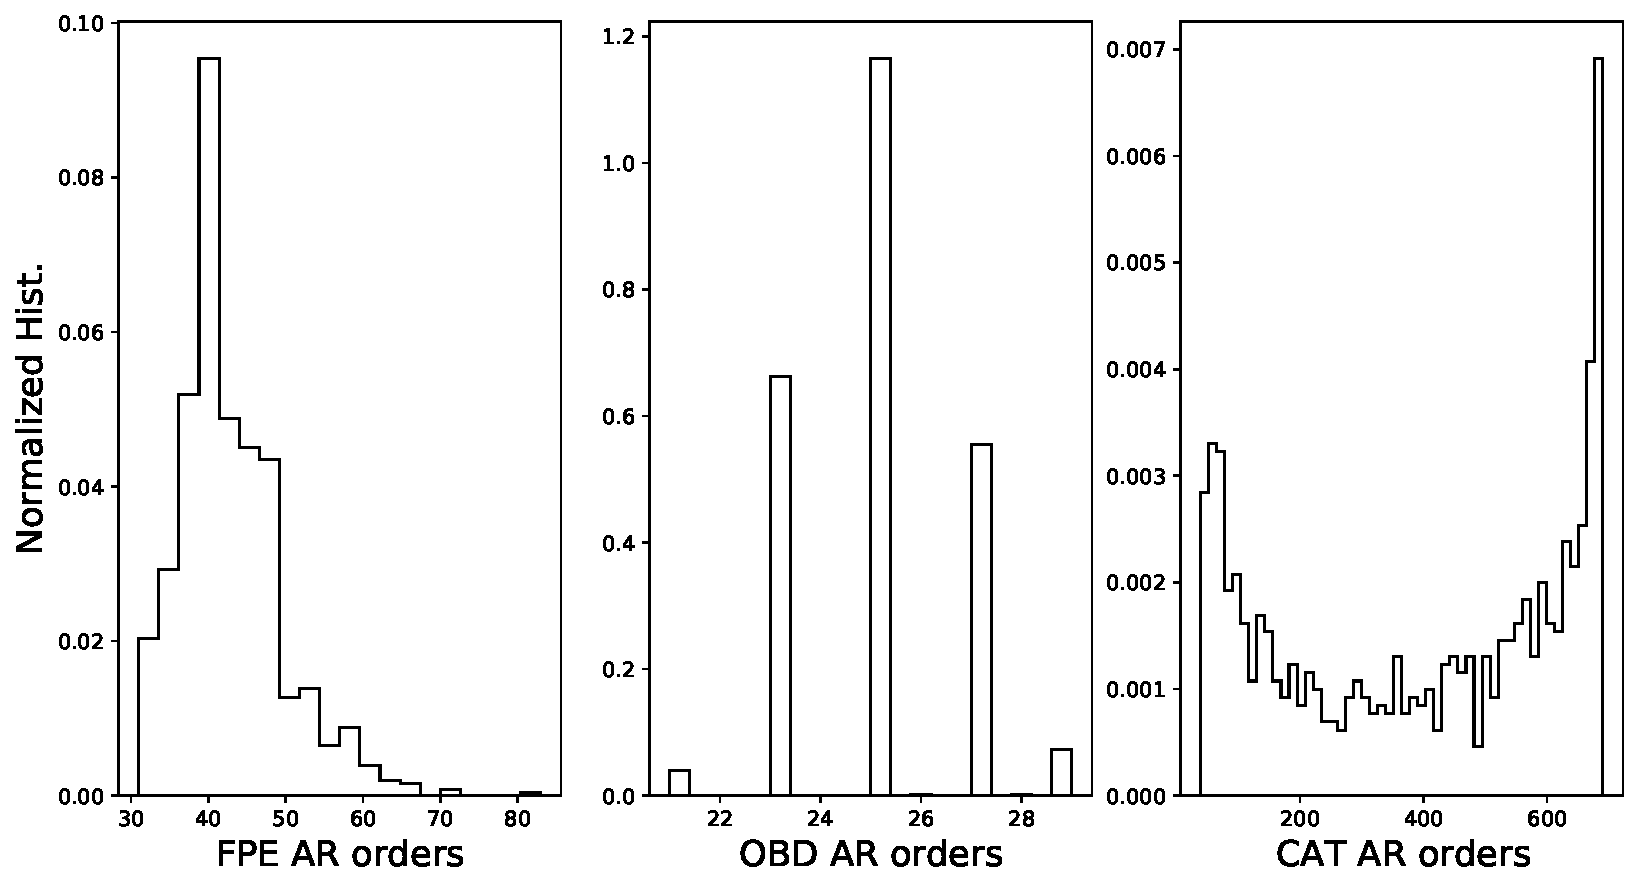
\includegraphics[width = \linewidth]{Images/NormalPSD/ordersComparison.pdf}
    \caption{Histogram of estimate orders for each method}
    \label{fig:ordersCompairson}

\end{figure}
definitely shows that FPE gives the best results: it is a stable method that choose filters in the clustered area associated with minimum error, while both OBD and CAT result lies outside this area and show bigger errors. Two other interesting plots that stress this fact are reported in figure \ref{fig:ordersCompairson} and \ref{fig:residualsComparison}
\begin{figure}
    \centering
    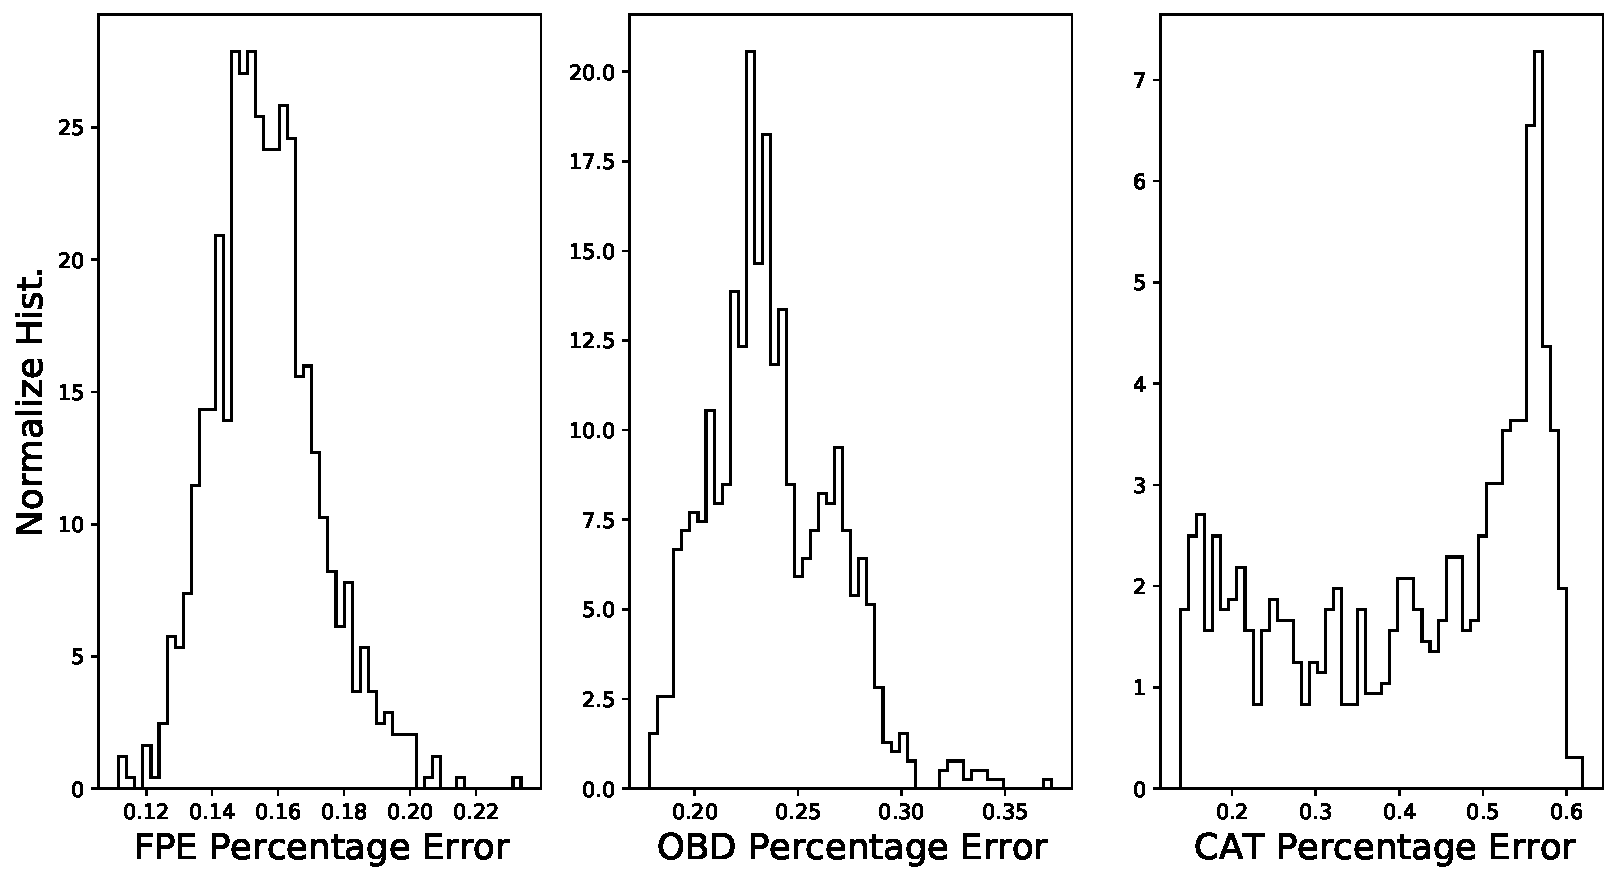
\includegraphics[width = \linewidth]{Images/NormalPSD/ResidualsComparison.pdf}
    \caption{Histogram of residuals for each method}
    \label{fig:residualsComparison}
\end{figure}
where the histograms for the errors and for order's estimate are reported. These graphs provide stronger evidence for our previous statements. As already noticed, FPE is very stable and provide the smallest 'overall relative error'. \\
CAT histogram shows a very interesting behaviour. The histogram for the order show two different peaks,  a small one associated to 'short filters', and a second high peak at $m = M$. This means that CAT is most likely to not converge at all at some value for the regression order, and it is more likely selects a length that is comparable with the largest available.  If short filters are selected, the overall percentage error will be low, respectively represented by the first peak in the distribution of the errors, while if long filters are selected, the error is maximized. 

So, even if in some cases CAT might be more accurate when taking the average over several spectra, FPE guarantees that minimum error will be reached. 

\subsection{Choosing an optimizer - LIGO Spectrum} \label{sec:LIGO_validation}
\begin{figure}
    \centering
    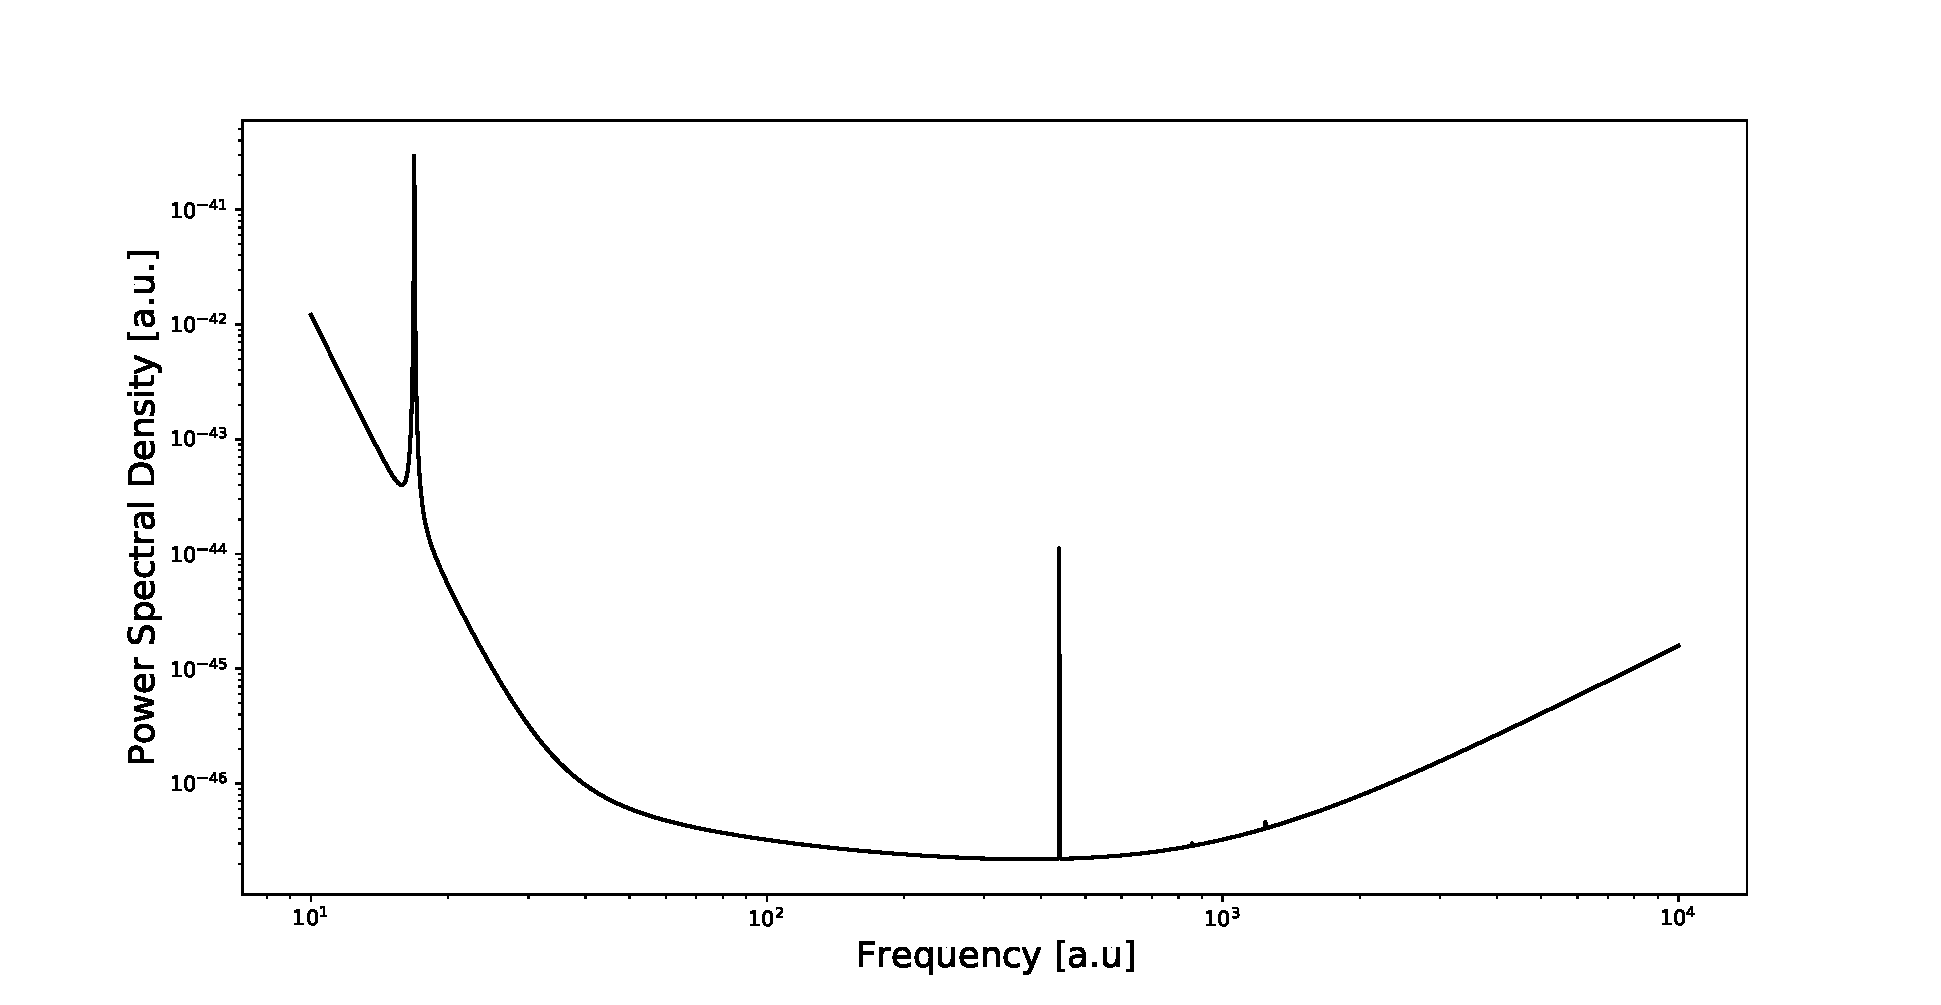
\includegraphics[width = \linewidth]{Images/LIGOsimulate/LigoPSDoriginal.pdf}
    \caption{Original power spectral density from Ligo}
    \label{fig:LigoPSDOriginal}
\end{figure}
In this subsection we concentrate again on the reconstruction of a specific, known, power spectrum.
We analyze the properties of reconstruction of this second spectrum whose shape is the Advanced LIGO design sensitivity theoretical spectral curve (Figure \ref{fig:LigoPSDOriginal}). 
For this analysis we will study properties only for arrays of 40960 points. We consider a sampling rate of $2048 samples / second$ that means we can reconstruct a Nyquist frequency of $1024 Hz$. We chose a longer dataset than before because algorithm works with a 1 dimensional interpolation of spectrum, and with shorter datasets the interpolated spectrum is not consistent with the original spectrum and does not capture the height of the peaks. Shorter choices would result in noise extracted from a different power spectrum than the one in figure \ref{fig:LigoPSDOriginal}. \\ 
We will study statistical properties from samples obtained with 500 simulations and compare the obtained results for each optimizer. 
We start considering statistical properties of mean spectrum obtained averaging over all the simulations and conclude with an analysis for the statistics of the reproduction of single spectrum. 
\subsubsection{Properties for the average spectrum}
Here we report mean properties of the reproductions of the spectrum. The spectrum we want to reconstruct is reported in Figure \ref{fig:ligospectrum},
\begin{figure}
    \centering
  
        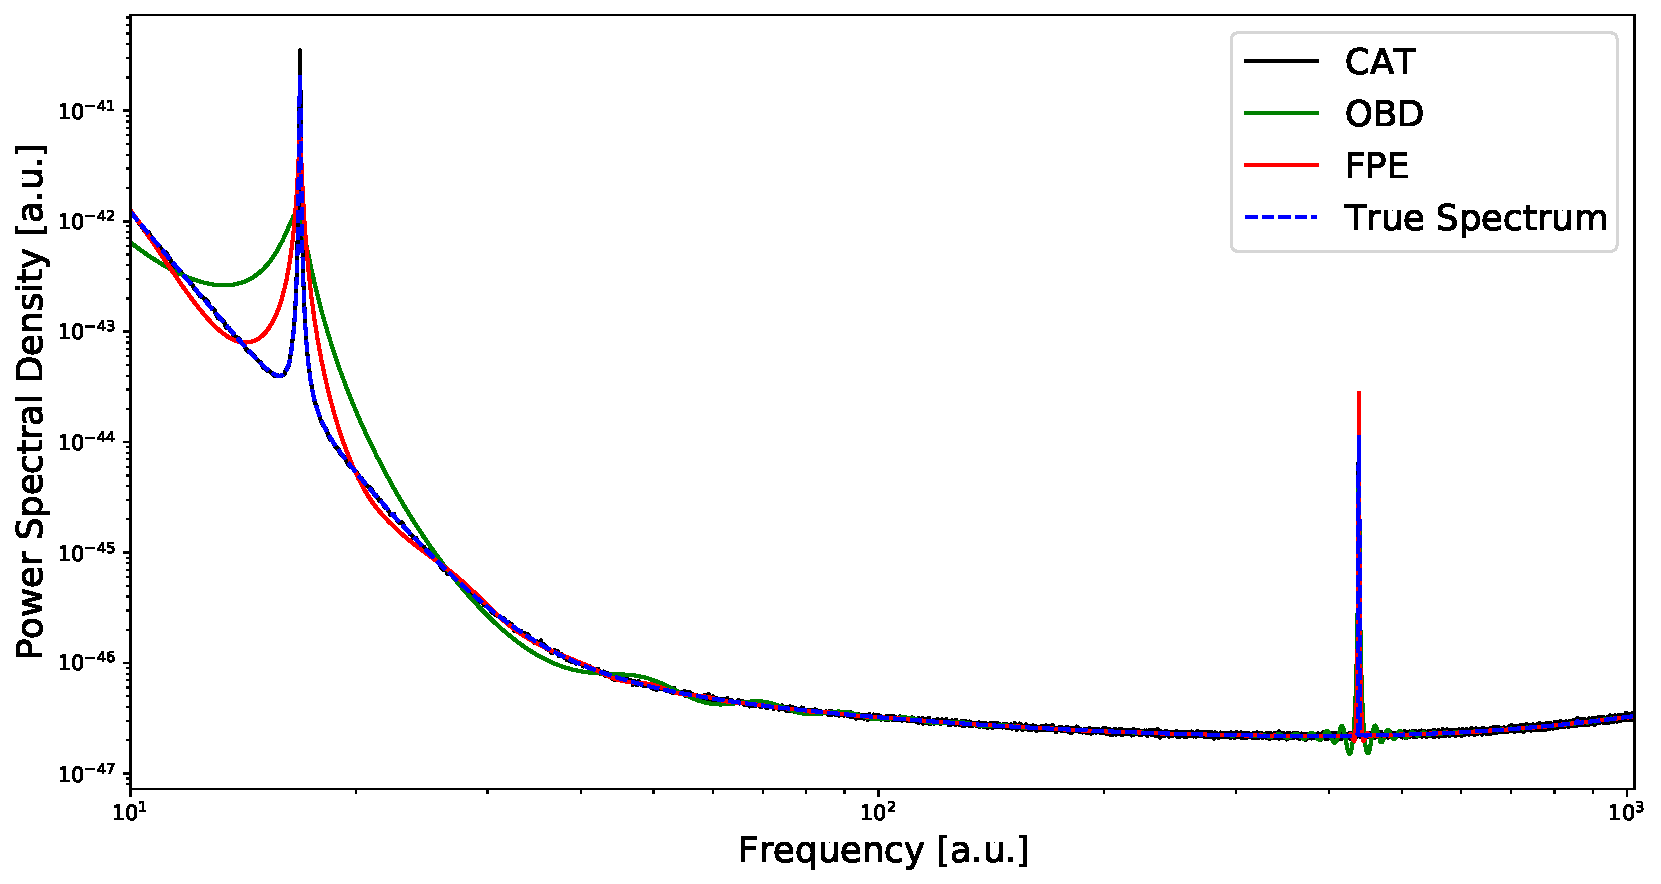
\includegraphics[width = \linewidth]{Images/LIGOsimulate/PSD.pdf}
        \caption{A priori spectrum from Ligo database}
        \label{fig:ligospectrum}
\end{figure}
shows the original power spectral density and the ensemble average of every method. For the mean, the relative errors are: 
\begin{equation}
    \bar r_{\bar S, FPE} = 0.0426\%, \qquad \bar r_{\bar S, OBD} = 0.129\%, \qquad \bar r_{\bar S, CAT} = 0.0211\%
\end{equation}
Again, if one only check overall accuracy for every method, CAT is outperforming. In fact, even in presence of very sharp peaks, CAT reconstruction seems to be almost perfectly coincident with each of them. To check this behaviour we take a look at the two peaks separately. For the first one a log plot of the reconstructed peaks and their relative errors are shown in Figure \ref{fig:ligo1peak} 
\begin{figure}[h]
        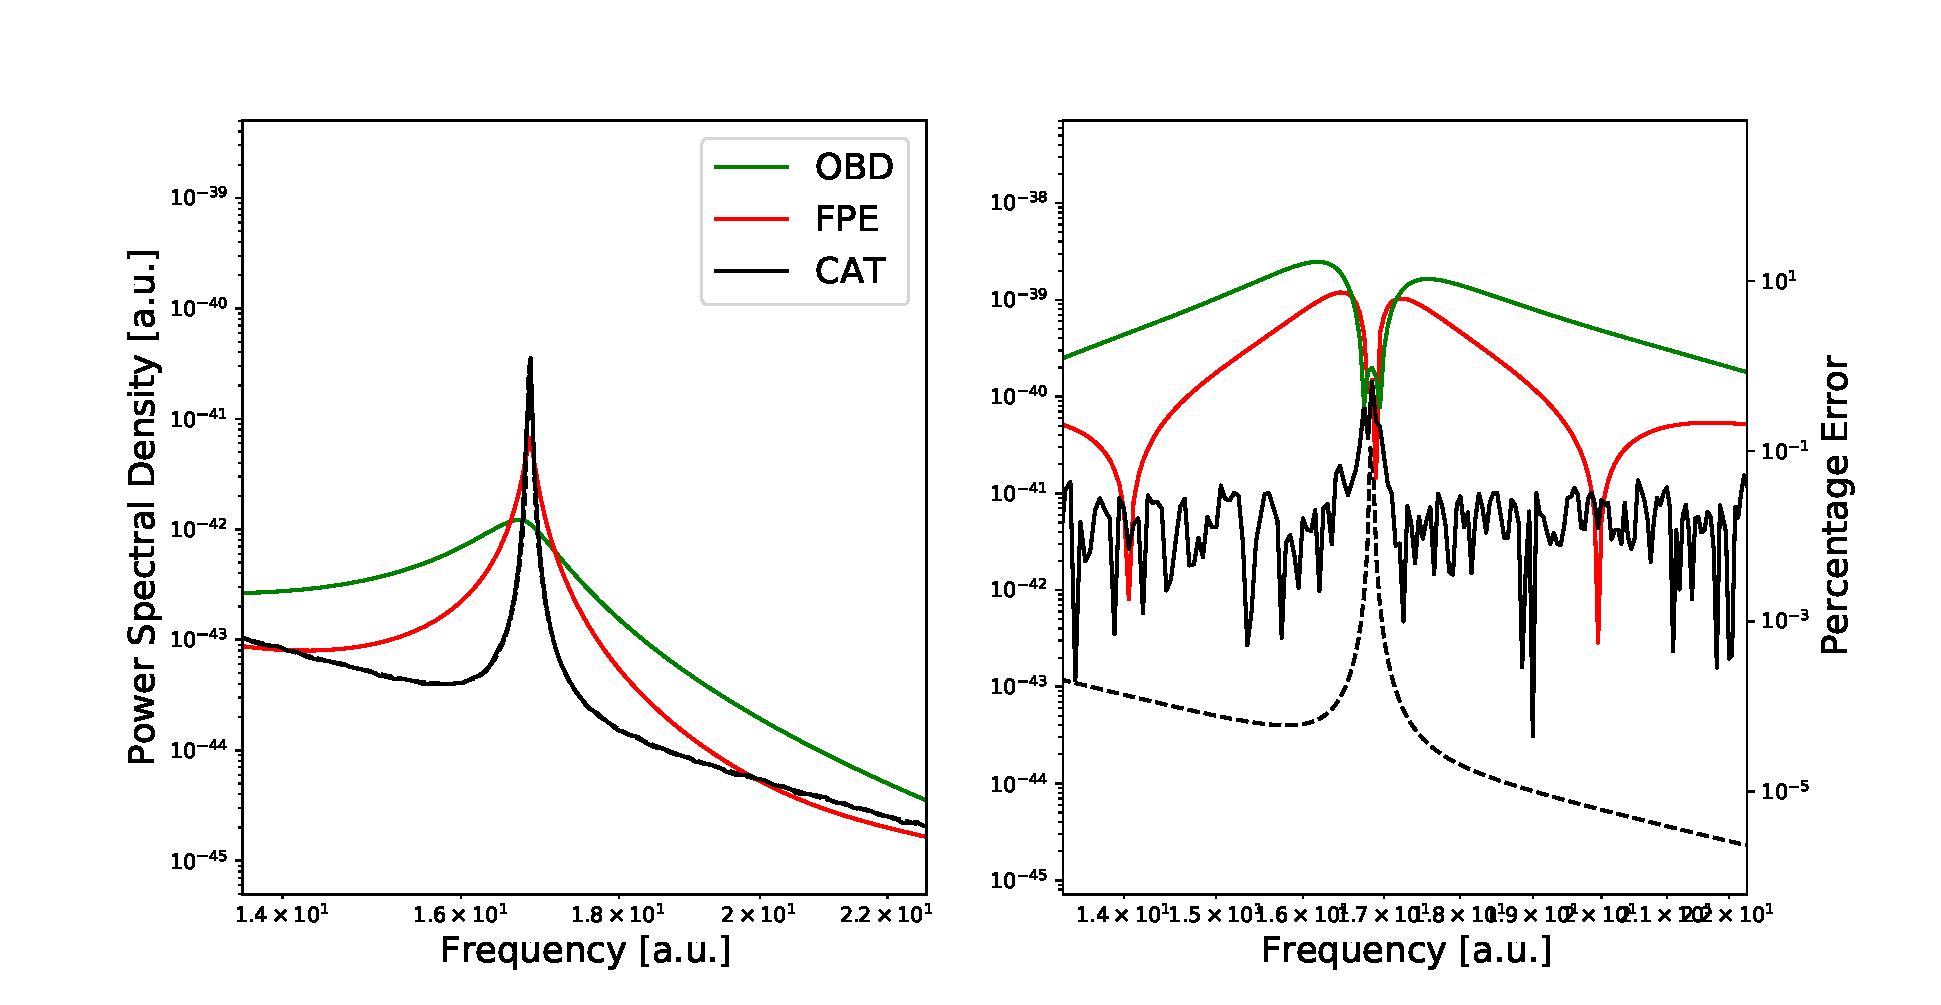
\includegraphics[width = \linewidth]{Images/LIGOsimulate/1stPeakComparison.pdf}
        \caption{1st peak of the spectrum and it reconstruction with every optimizer (left) and associated percentage error (right)}
        \label{fig:ligo1peak}
\end{figure}
and the results reinforce our previous statement. The behaviour of the error is very similar for CAT and FPE, showing similar shapes but very different sizes, while CAT is giving a different and way more precise result. Both FPE and OBD are not able to capture the width of the peak and also show larger errors, while CAT has a good behaviour in reconstructing width's also. 
The reconstruction for very sharp peaks considering the average over all the spectra is found to be strongly inaccurate for both FPE and OBD, while a good accuracy is reached with CAT method. \\ 
Considering the estimate for the position of the peak, whose true value is found to be $16.85 \quad a.u. $, within numerical accuracy both FPE and CAT find its exact position, while OBD shift the peak left at $16.7 a.u.$, with a $0.9\%$ inaccuracy.\\ 
Second peak results are analogous, plotting the peak and the errors value around it
\begin{figure}[h]
    \centering
        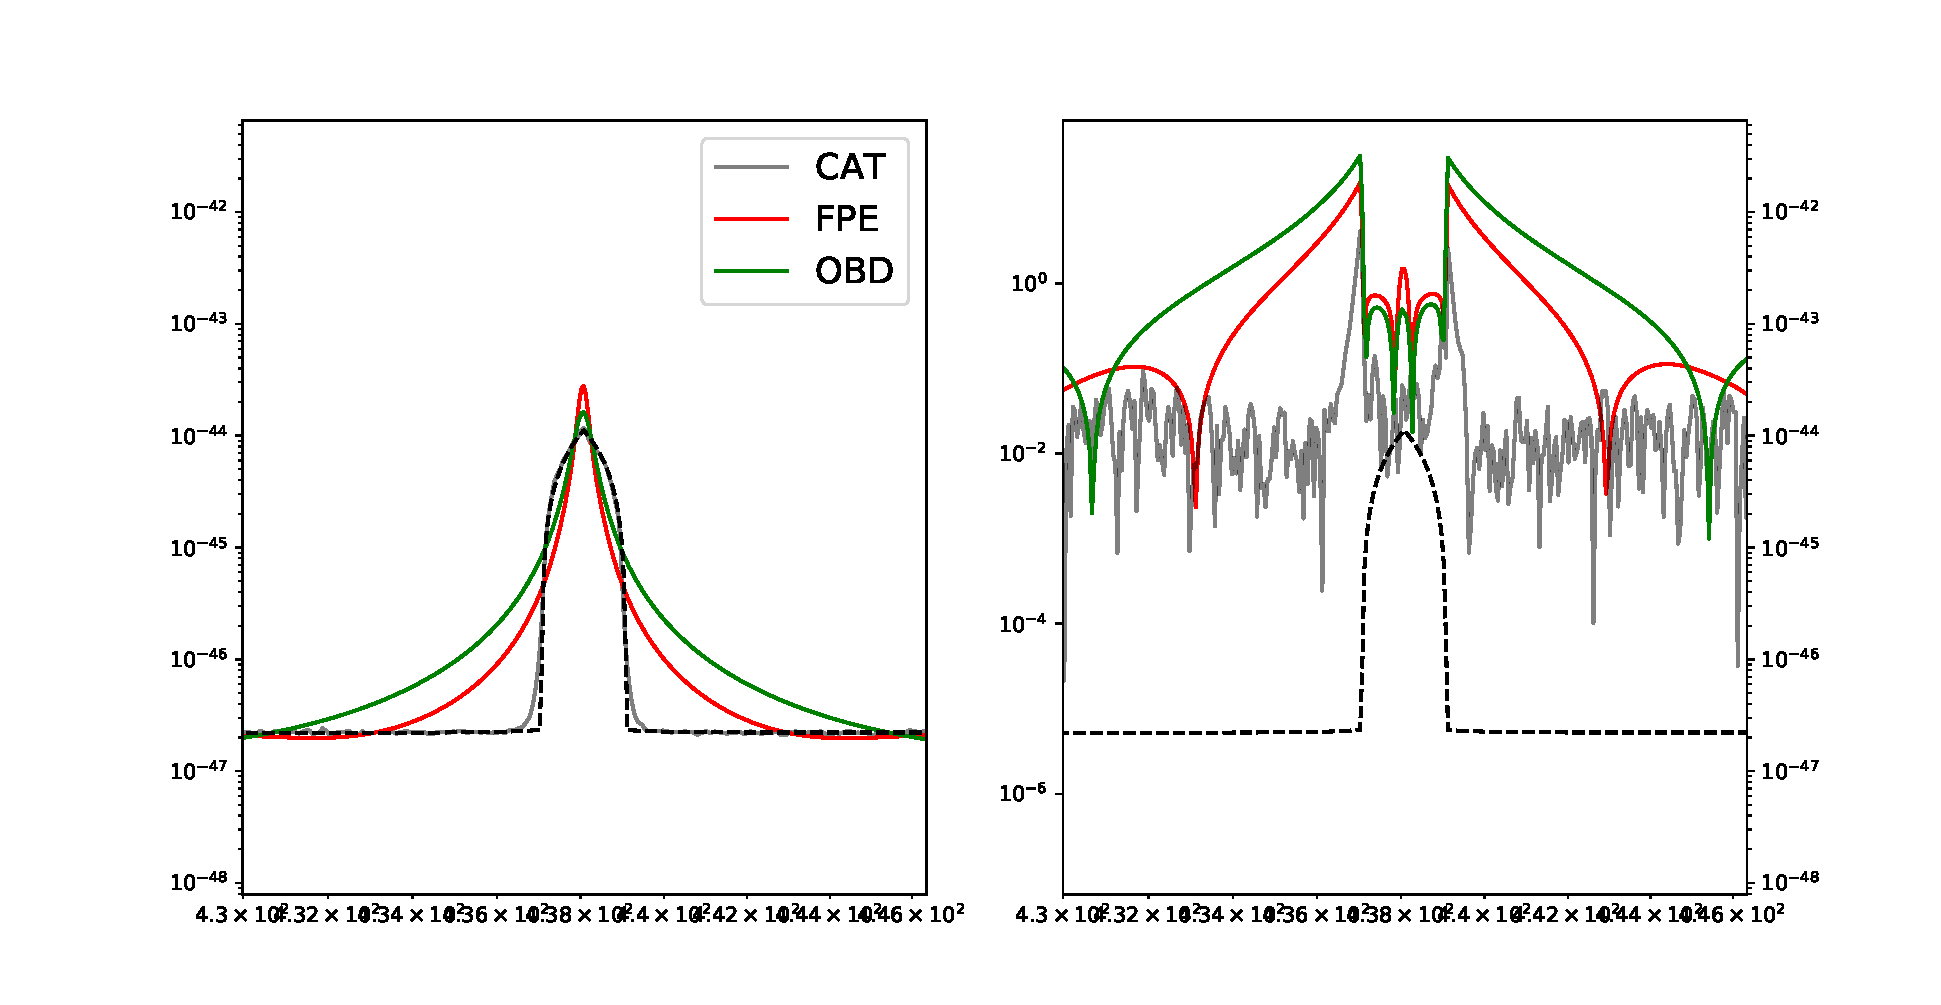
\includegraphics[width = \linewidth]{Images/LIGOsimulate/2ndPeakComparison.pdf}
        \caption{2nd peak of the spectrum, Relative error around 2nd peak of the spectrum}
        \label{fig:ligo2peak}
\end{figure}
we find again that FPE and OBD are performing similarly, the magnitude of the error is maximum for OBD and minimum for CAT. \\ 
In this case even CAT shows large errors in some points, but they are reasonable in a large part of it, still, it remains the best reconstruction.  For this second peak, all the methods find maximum position to be at $438.05 \quad a.u.$, which is the true position of the maximum.
Looking at Figure \ref{fig:ligo1peak} at \ref{fig:ligo2peak}, it appears to be clear that the least of the accuracy is not on the peak, but immediately around, so that one of the biggest deal is the reconstruction of peak's width, that only CAT is able to capture with high definition. \\ 
Even if FPE shows larger error in the peaks than CAT, when the average over all the frequencies is considered, their percentage errors are of the same order of magnitude. This means that outside the peaks FPE is more accurate than CAT, i.e. CAT is still giving noisy results.\\ 
As for the normal distributed noise, mean spectrum is not sufficient to declare what is the best optimizer to be used, since most of experiment are purely observational and mean spectrum over different realizations of the same stochastic process cannot be computed. So, it is important to also understand what is their behaviour for single realizations of the process.
\subsubsection{Statistical properties of single realizations} 
The errors for the single realizations behave very differently from the errors obtained when we considered the mean spectrum. In computing the mean of the overall errors for each single spectrum, the results we obtain are the following:
\begin{equation}
    \bar{r}_{FPE} = 0.13 \pm 0.01; \qquad \bar{r}_{OBD} = 0.17 \pm .02; \qquad 
    \bar{r}_{CAT} = 0.4 \pm 0.1
\end{equation}
where the error is just the standard deviation of the samples.
In this case we find a different result: FPE shows the best results and order's estimate is associated with least errors. Also, having found a smaller standard deviation of the datas, we can state that FPE and OBD are more stable optimizers then CAT. In fact, their properties as a function of filter's length are almost identical to those obtained in the study of normal spectrum. If we again plot the value of the errors as a function of the estimate of the order (Figure \ref{fig:LigoOrderError})
\begin{figure}
    \centering
    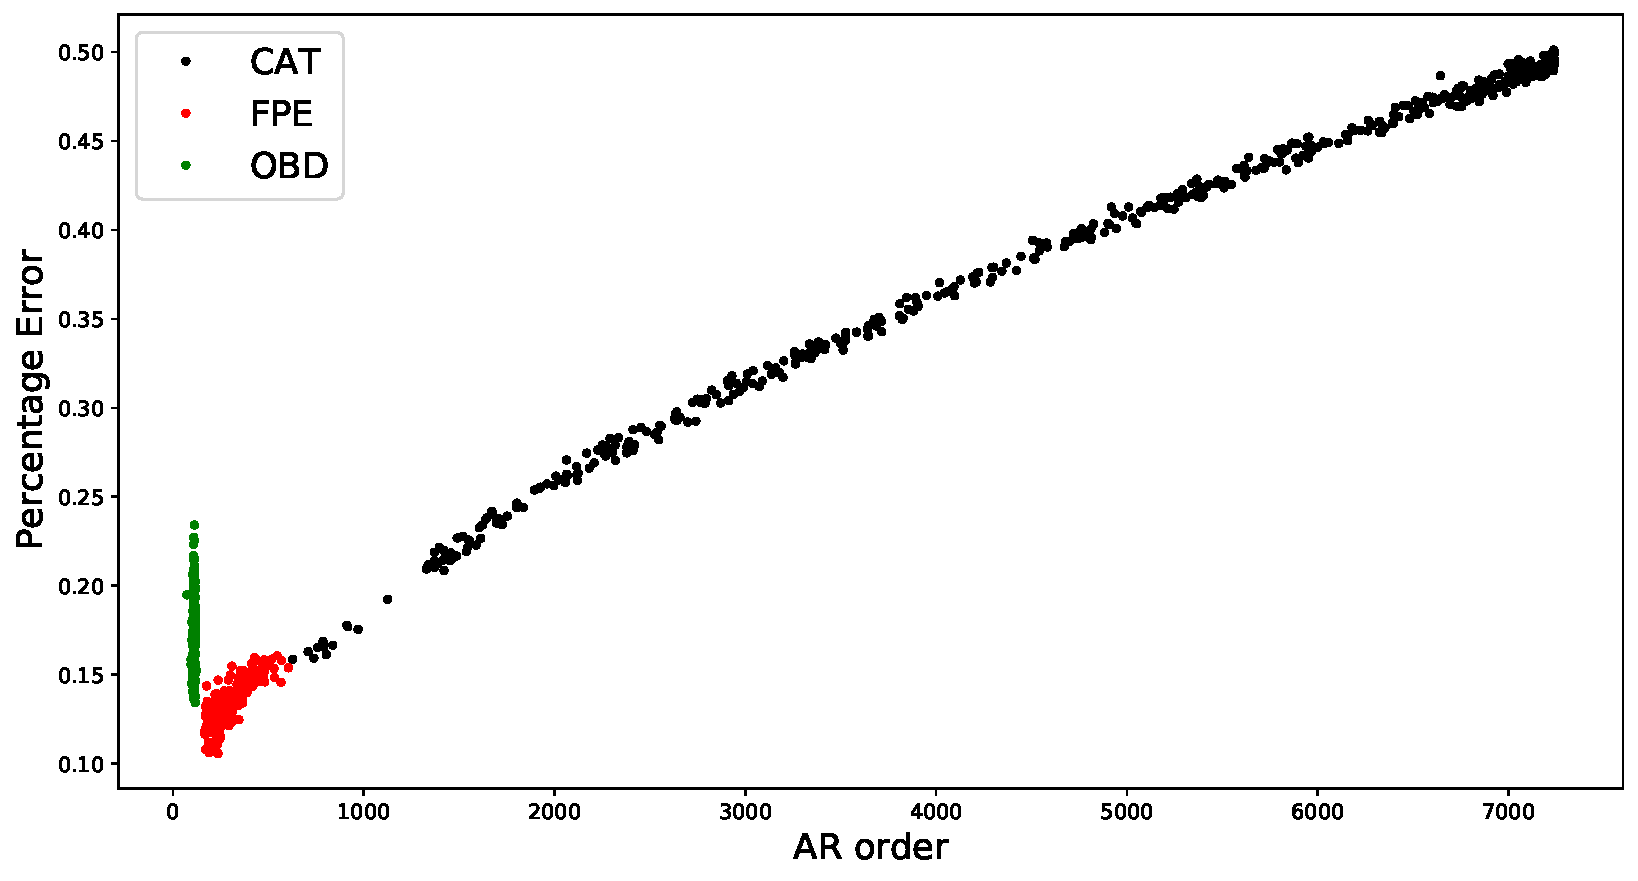
\includegraphics[width = \linewidth]{Images/LIGOsimulate/orderVSerror.pdf}
    \caption{Plot of relative error as a function of the estimate for filter's length}
    \label{fig:LigoOrderError}
\end{figure}
it is immediate to see that, again, FPE results lies in the are of filter's length associated with a minimum of relative errors, OBD lies in a clustered window with a higher error and CAT is not convergent, but most of the results are outside the minimum error area. So, we arrive at the same conclusion we had when we considered the normal specturm. OBD has no general properties that make it a preferable optimizer then FPE or CAT while, what to choose beneath the last two is based on the problem we are dealing with: if we have one single realization for the process, we are mostly sure that FPE would catch the area associated with the best resolution possible, while CAT would result in a spurious result with, in general, a not so good resolution. But, in case we have several realization for the same process, this last property of CAT, together with its instability, result to be his luck and, taking the average errors tend to compensate noise in the result, originating a very well defined spectrum that show same resolution almost everywhere, no matter how small the values are (as for normal PSD case) or how sharp peaks can be, the result has got generally good accuracy, also if it is clear that we have to pay this fact with very large error bars. So a choice between these methods is a matter of convenience and interest for each specific problem. \\
\begin{figure}
    \centering
    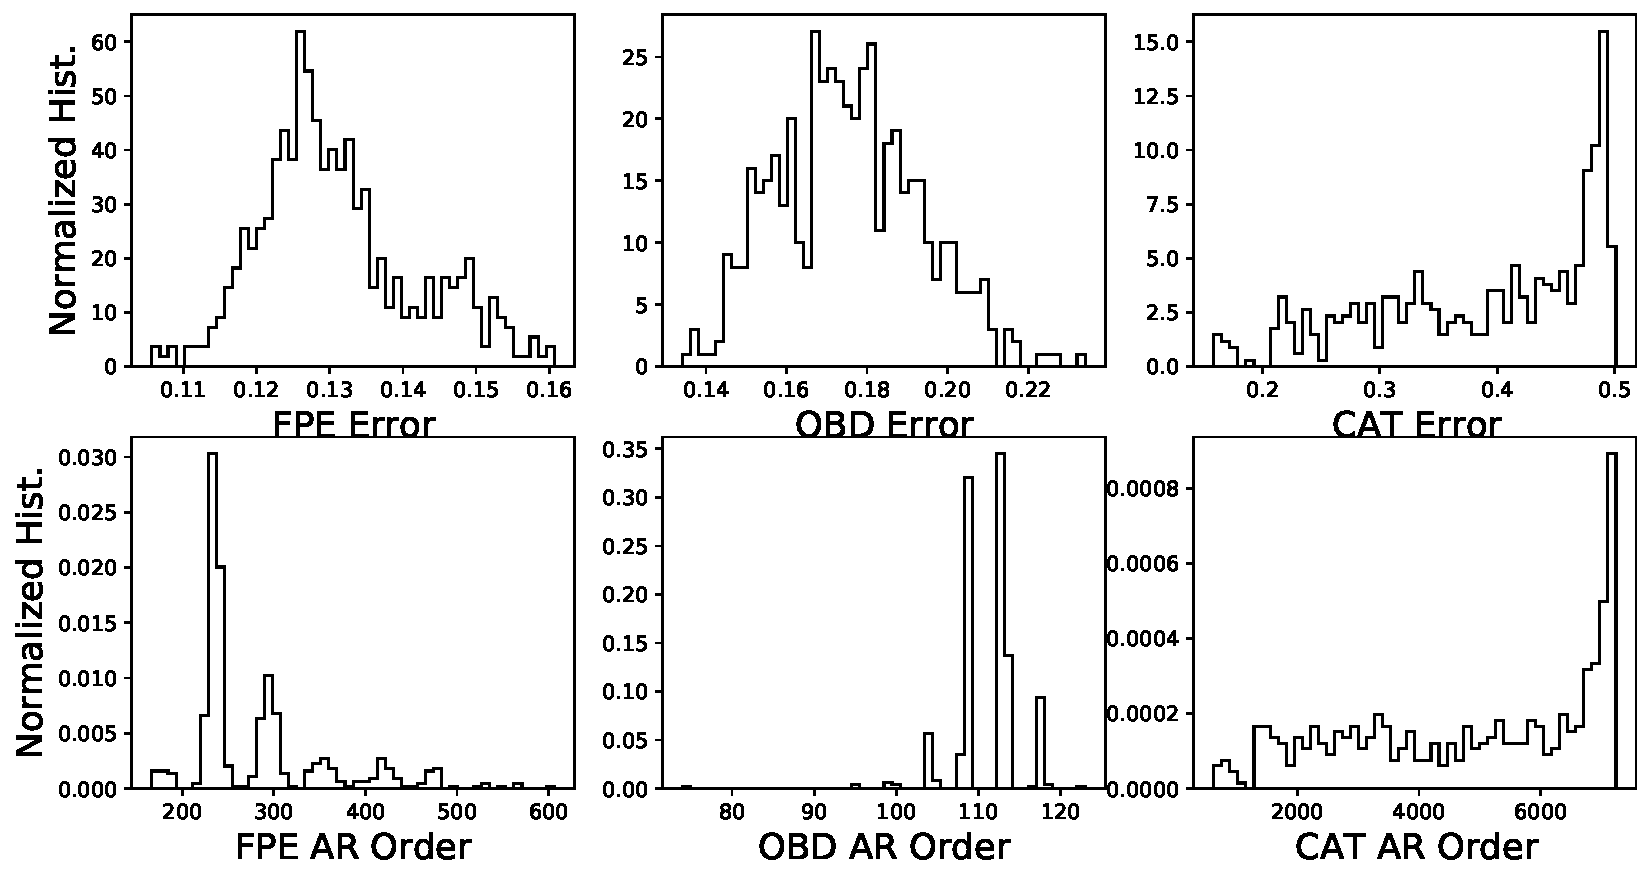
\includegraphics[width = \linewidth]{Images/LIGOsimulate/LigoHists.pdf}
    \caption{Histograms showing the estimate for the autoregressive order and overall percentage error obtained with all the three optimizers.}
    \label{fig:my_label}
\end{figure}

\section{Comparison with Welch method}

It is really interesting to have a qualitative comparison between the performance of the MESA and of the standard Welch algorithm.
We perform such comparison on the spectrum of LIGO (even though similar conclusions can be drawn from any other shape of the PSD).

We perform two sets of experiments.
In the first one (see fig.~), we simulate data from an analytical PSD and we make the comparison with them: this is to endure the we have a baseline PSD to compare the data with.
In a second experiment (see fig.~), we employ the data released to the public byt the LIGO/Virgo collaboration.
In each experiment, we vary the length of the data used for the estimation: this is also useful to assess how the computation depends on the data available. We set the total observation time $T = 1, 5, 10, 100, 1000 \SI{}{s}$
For the MESA algorithm, we employ FPE optimizer. For the Welch algorithm, we employ a Tukey window, an overlap fraction of $0.5$ for the segments and a length of segments $L = 512, 1024, 2048, 8192, 32768$ datapoints.
In all cases, the sampling rate is set to $\SI{4096}{Hz}$.

First of all, we note that using a longer time series results in a more stable estimation of the PSD, especially in the low frequency sector. This is somehow obvious: more data provide more information available for spectral estimation. This fact is more important at lower frequencies, where the natural time length is large.
Turning to the comparison between MESA and Welch's method, we find that the PSD estimation provided by the Welch's method is more noisy (i.e. has a large number of spurious peaks) rather than PSD provided by MESA. The different behavior is more manifest in the low frequency sector.
The result does not change much by changing the hyperparameters required for Welch algorithm.
\sschmidt{Other observations??}


\begin{figure}
	\label{fig:mem_welch_realdata}
	\caption{Blablabla}
\end{figure}

\sschmidt{Mettiamo da qualche parte una descrizione dettagliata del codice?}

\section{Final remarks and future prospects}

\appendix
\section{MESA solution} \label{sec:MESA_solution}
\subsection{MESA solution}
We will follow the solution proposed by Burg in his PhD thesis \cite{burg1975maximum}. Instead of directly solving the variational problem for the power spectral density, we will rewrite it in terms of the constraints (\ref{eq:MaxConstraint}) of the problem. $S(f)$ is defined as the Fourier Transform of the autocorrelation function, as: 
\begin{equation}
    S(f) = \frac{1}{2 Ny}\sum_{n = -\infty}^{\infty} \bar r_n e^{- \imath 2 \pi n \Delta t}.
\end{equation}
Substituting in \ref{eq:EntropyGain2}, the variational problem reduces to the maximization of: 
\begin{equation}
    \int_{-Ny}^{Ny}  
    \log\left(\frac{1}{2 Ny}\sum_{n = -\infty}^{\infty} \bar r_n e^{-\imath 2 \pi f n \Delta t} 
    \right) df.
\end{equation}
As we said before, not all the values for the autocorrelation are known. Generally, we have access to a finite number of values for the autocorrelation function, ranging in a symmetric interval $n \in [-N, N]$. 
In the previous equation, since the summation index is ranging between $-\infty$ and $+\infty$, we are correctly assuming that also the unknown values have to be used in the computation of the power spectral density. But, since they are not known, we have to require the maximization of entropy to be independent of these values:
\begin{equation}\nonumber 
    \frac{\delta H}{\delta \bar r_s} = 0 \text{ for } \vert s \vert > N. 
\end{equation}
Using the explicit form for $H$, this becomes
\begin{equation}
      \frac{\delta H}{\delta \bar r_s} = \frac{1}{2Ny}\int_{-Ny}^{Ny} S(f)^{-1}e^{-\imath 2 \pi f s \Delta t } df = \lambda_s = 0 \text{ for } \vert s \vert > N. 
\end{equation}
We see that $S(f)$ can be expressed in terms of the $\lambda s$ via a Fourier Series
\begin{equation}\label{eq:PSDconstraint}
    S(f)^{-1} = \sum_{s = -N}^N \lambda_s e^{-\imath 2 \pi f s \Delta t},
\end{equation}
This is a non-linear closed expression for the power spectral density. The requirement for $S(f)$ to be positive definite implies that: 
\begin{equation}
    \nonumber 
    \lambda_{-s} = \lambda_s^* 
\end{equation}
With this property, and defining $z = e^{-\imath 2 \pi f \Delta t}$, $S(f)^{-1}$ can be rewritten as a polynomial in $z$ and $z^*$
\begin{equation}
    \label{eq:zExp}
    S(f)^{-1} = \lambda_0 + \sum_{s = i}^N \lambda_s z^s + \sum_{s = 1}^N \lambda^*_s z^{-s}.
\end{equation}
Let $z_0$ be a root for the polynomial
\begin{equation}
    \nonumber
    \lambda_0 + \sum_{s = 1}^N \lambda_s z_0^s + \sum_{s = 1}^N \lambda^*_s z_0^{-s} = 0,
\end{equation}
it is easy to show that $(z_0^*)^{-1}$ is also a root for the equation: 
\begin{align}
    \nonumber 
    &\lambda_0 + \sum_{s = 1}^{N} \lambda s \left(\frac{1}{z_0^s} \right)^* + \sum_{s = 1}^N \lambda^*_s \left(\frac{1 }{z_0^{-s}}\right)^* = \\ \nonumber 
    &\lambda_0 + \sum_{s = 1}^N \lambda_s (z_0^{-s})^* + \sum_{s=1}^N \left(\lambda_s (z_0^s)\right)^* = \\ \nonumber 
    &\left(\lambda_0 + \sum_{s=1}^N \lambda_s z_0^s + \sum_{s = 1}^N \lambda^*_s z_0^{-s}\right)^* = 0 
\end{align}
This means that for every pole $z_0$ laying outside (inside) the unit circle, there is another pole inside (outside) the unit circle.  So, if there are no roots on the unit circle, $N$ roots lay outside and $N$ inside of it. \\ 
These properties allow us to rewrite the Fourier expansion (\ref{eq:zExp}) as \cite{1975STIN...7714318B}
\begin{equation}\nonumber 
    S(f)^{-1} = \frac{1}{P_N \Delta t} \left(1 + \sum_{s}^N a_s z^s\right)\left(1 + \sum_s^N  a^*_s z^{-s}\right),
\end{equation}
or, defining $a_0 = 1$,
\begin{equation}\label{eq:MESApsd_appendix}
    S(f) = \frac{P_N \Delta t}{\left(\sum_{s=0}^N a_s z^z\right)\left(\sum_{s = 0}^N a^*_s z^{-s}\right)}. 
\end{equation}
The MESA expression for the power spectral density admits a non-linear, all pole representation when evaluated in $z = e^{-\imath 2 \pi f \Delta t}$. All the roots of the first polynomial can be chosen to lay outside the unit circle, so that all the roots of the second polynomial will lay inside of it \cite{1975STIN...7714318B}. 
If one is able to compute the values of the coefficients $a_i$ the PSD is uniquely determined from the previous equation. \\ 
To compute the $a_i$-s, we substitute in equation
(\ref{eq:MaxConstraint}) with the above representation for $S(f)$ in terms of the $a_i$ coefficients. Changing  variable from $f$ to $z(f) = e^{-\imath 2 \pi f \Delta t}$, the integral (\ref{eq:MaxConstraint}) becomes a contour integral in the unit circle centered at the origin of the complex plane: 
\begin{equation}
   \frac{P_N}{2 \pi \imath} \oint _{\mathbb S^1}\frac{z^{-s - 1}}{\sum_{n = 0}^N a_n z^n \sum_{n = 0}^N a^*_n z^{-n}}dz = \bar r_s. 
\end{equation}
Sending $s \to s - r$, multiplying by $a^*_s$ and summing over all possible values for $s$ the equation becomes 
\begin{align} \nonumber 
    \sum_{s = 0}^N a_s \bar r_{s - r} &= \frac{P_N}{2 \pi \imath}\oint \frac{z^{r - 1} \sum_{s = 0}^N a^*s z^{-s}}{\sum_{s = 0}^N a_s z^s \sum_{s = 0}^N a^*s z^{-s}} dz\\
    & = \frac{P_N}{2 \pi \imath}\oint \frac{z^{r -1}}{\sum_{s = 0}^N a_s z^s}dz\label{eq:ErFilter}
\end{align}
Since all the zeros of the denominator lay outside the unit circle, the contour integral is 0. The only exception is for $r = 0$ with a residual in the origin of the axis. For $r = 0$ the integral can be computed via the Cauchy integral formula and (\ref{eq:ErFilter}) becomes: 
\begin{align}\label{eq:errorFilter1}
    \sum_{s = 0}^N a_s \bar r_{r - s} &= P_N \quad \text{ if } r = 0 \\ \label{eq:errorFilter2}
    \sum_{s = 0}^N a_s \bar r_{r - s} & = 0 \qquad \text{ if } r \neq 0.
\end{align}
This kind of equations are solved by the use of the Levinson recursion \cite{doi:10.1002/sapm1946251261}
\subsection{Levinson Recursion}
The equations (\ref{eq:errorFilter1}) and (\ref{eq:errorFilter2}) can be rewritten as a Matrix equation of the form
\begin{equation}\label{eq:predictionErrorFilter}
    \begin{pmatrix}
    \bar r_0 &  \bar r_{-1} & \dots & \bar r_{-N}\\
    \bar r_{1} & \bar r_ 0 & \dots & \bar r_{1 - N} \\ 
    \bar r_{2} & \bar r_{1} & \dots & \bar r_{2 - N}
    \\
    \vdots & \vdots & \ddots & \vdots  \\
    \bar r_{N} & \bar r_{N - 1} & \dots  &\bar r_0
    \end{pmatrix}
    \begin{pmatrix}
    1 \\   a_1 \\   a_ 2 \\  \vdots \\   a_N
    \end{pmatrix} = 
    \begin{pmatrix}
    P_N \\   0 \\  0 \\ \vdots  \\   0
    \end{pmatrix}
\end{equation}
know as the prediction error filter equation. It is a matrix equation involing the Toeplitz Matrix $R_{ij}$ and the vector $\vec a$, known as the forward prediction error filter. The approach for solving the equations is the Levinson - Durbin recursion. \\
Our goal is to obtain the $N$-th order equation (\ref{eq:predictionErrorFilter}) from the $N-1$-th order equation: 
\begin{equation}\label{eq:Forward}
    \begin{pmatrix}
    \bar r_0 & \bar r_{-1} & \dots &\bar r_{1 - N}\\
    \bar r_{1} & \bar r_0 & \dots & \bar r_{2 - N} \\ 
    \vdots & \vdots & \ddots & \vdots \\ 
    \bar r_{N - 1} & \bar r_{N -2} & \dots & \bar r_0
    \end{pmatrix} 
    \begin{pmatrix}
    1  \\   b_1  \\  \vdots \\   b_{N - 1}
    \end{pmatrix} =
    \begin{pmatrix}
    P_{N -1} \\  0 \\ \vdots \\ 0
    \end{pmatrix} .
\end{equation}
This equation is not sufficient to solve the recursion. Since the autocorrelation matrix is self-adjoint, from equations (\ref{eq:errorFilter1}) and (\ref{eq:errorFilter2}) and noting that the first and the last row of the autocorrelation matrix are respectively the complex conjugate reverse, is easy to show that
\begin{equation}\label{eq:Backward}
     \begin{pmatrix}
    \bar r_0 & \bar r_{-1} & \dots &\bar r_{1 - N}\\
    \bar r_{1} & \bar r_0 & \dots & \bar r_{2 - N} \\ 
    \vdots & \vdots & \ddots & \vdots \\ 
    \bar r_{N - 1} & \bar r_{N -2} & \dots & \bar r_0
    \end{pmatrix} 
    \begin{pmatrix}
    b^*_{N-1} \\ b^*_{N- 2} \\\vdots \\ 1
    \end{pmatrix} 
    = 
    \begin{pmatrix}
    0 \\ 0 \\ \vdots \\ P_{N-1}
    \end{pmatrix} 
\end{equation}
holds. The vector obtained reflecting b and taking its complex conjugate is known as ``backward prediction error". \\ 
Stepping from order $N - 1$ to order $N$, the autocorrelation matrix grows from size $(N,N)$ to size $(N + 1, N + 1)$, this implies that a new component $b_n$ for the prediction error filter is needed. If we take it to be $b_N = 0$, this choice does not modify the first $N$ component of the right side of equation (\ref{eq:Forward}) (or the last $N$ components of (\ref{eq:Backward})), i.e.:

\begin{equation}\label{eq:OrderN}
    \begin{pmatrix}
    \bar r_0 & \bar r_{-1} & \dots &\bar r_{1 - N} & \bar r_{- N}\\
    \bar r_{1} & \bar r_0 & \dots & \bar r_{2 - N} & \bar r_{1 - N}\\ 
    \vdots & \vdots & \ddots & \vdots & \vdots \\ 
    \bar r_{N -1} & \bar r_{N-2} & \dots & \bar r_0 & \bar r_{-1}
    \\
    \bar r_{N } & \bar r_{N -1} & \dots & \bar r_1 & r_0 
    \end{pmatrix} 
    \begin{pmatrix}
    1  \\   b_1  \\  \vdots \\   b_{N - 1} \\ 0 
    \end{pmatrix} =
    \begin{pmatrix}
    P_{N -1} \\  0 \\ \vdots \\ 0 \\ \Delta_N
    \end{pmatrix} .
\end{equation}
with 
\begin{equation}
    \Delta_N = \sum_{n=0}^N \bar r_{N - n}b_n.
\end{equation}
Adding the previous expansion for both forward and backward equations, one obtains 
\begin{equation}\nonumber 
        \begin{pmatrix}
    \bar r_0 & \bar r_{-1} & \dots & \bar r_{- N}\\
    \bar r_{1} & \bar r_0 & \dots & \bar r_{1 - N}\\ 
    \vdots & \vdots & \ddots & \vdots \\ 
    \bar r_{N -1} & \bar r_{N-2} & \dots &  \bar r_{-1}
    \\
    \bar r_{N } & \bar r_{N -1} & \dots  & r_0 
    \end{pmatrix} 
    \begin{pmatrix}
    1  \\   b_1  \\  \vdots \\   b_{N - 1} \\ 0 
    \end{pmatrix} 
    + c_N 
    \begin{pmatrix}
    0 \\ b^*_{N -1} \\ \vdots  \\ b_1 \\ 1 
    \end{pmatrix}
    =
    \begin{pmatrix}
    P_{N -1} \\  0 \\ \vdots \\ 0 \\ \Delta_N
    \end{pmatrix} .
    + c_N
    \begin{pmatrix}
    \Delta^*_N \\ 0 \\\vdots \\ 0 \\ P_{N-1}
    \end{pmatrix}.
\end{equation}
With the reflection coefficient $c_N$ to be computed. Requiring the previous equation to be equivalent to \ref{eq:predictionErrorFilter}, one obtains
\begin{equation}\nonumber 
\begin{cases}
    P_{N - 1} + c_N\Delta^*_N = P_N \\
    c_N P_{N - 1} + \Delta_N = 0
\end{cases}
\end{equation}
which can be easily solved for $c_N$ and $P_N$ as 
\begin{equation}
    c_N = -\frac{\Delta_N}{P_{N-1}}; \quad \text{ and } P_N = P_{N - 1}\left(1 - \vert c_N \vert ^2 \right). 
\end{equation}
Having computed the value for the reflection coefficient, the $N$-th order forward prediction error filter is found to be 
\begin{equation}
    a_i = b_i + c_N b^*_{N - i}.
\end{equation}
To obtain the solution for the $N$-th order, one starts $\bar r_0 = P_0$ and recursively computes the new values until the desired order is computed. 
This problem is often solved numerically with Burg's Algorithm \cite{Vos}.


	\bibliography{Bibliography.bib}
	\bibliographystyle{ieeetr}

\end{document}


%%%%%%%%%%%%%% BELOW THE OLD PART... USEFUL TO TAKE INSPIRATION FROM

%%%%%%%%%%%%%%%%%%%%%%%%%%%%%%%%%

%%%%%%%%%%%%%%%%%%%%%%%%%%%%%%%%%

%%%%%%%%%%%%%%%%%%%%%%%%%%%%%%%%%

%%%%%%%%%%%%%%%%%%%%%%%%%%%%%%%%%

%%%%%%%%%%%%%%%%%%%%%%%%%%%%%%%%%

%%%%%%%%%%%%%%%%%%%%%%%%%%%%%%%%%

%%%%%%%%%%%%%%%%%%%%%%%%%%%%%%%%%

%%%%%%%%%%%%%%%%%%%%%%%%%%%%%%%%%

%%%%%%%%%%%%%%%%%%%%%%%%%%%%%%%%%

%%%%%%%%%%%%%%%%%%%%%%%%%%%%%%%%%

%%%%%%%%%%%%%%%%%%%%%%%%%%%%%%%%%

%%%%%%%%%%%%%%%%%%%%%%%%%%%%%%%%%

%%%%%%%%%%%%%%%%%%%%%%%%%%%%%%%%%

%%%%%%%%%%%%%%%%%%%%%%%%%%%%%%%%%

%%%%%%%%%%%%%%%%%%%%%%%%%%%%%%%%%

%%%%%%%%%%%%%%%%%%%%%%%%%%%%%%%%%

%%%%%%%%%%%%%%%%%%%%%%%%%%%%%%%%%

%%%%%%%%%%%%%%%%%%%%%%%%%%%%%%%%%

%%%%%%%%%%%%%%%%%%%%%%%%%%%%%%%%%

%%%%%%%%%%%%%%%%%%%%%%%%%%%%%%%%%

%%%%%%%%%%%%%%%%%%%%%%%%%%%%%%%%%

%%%%%%%%%%%%%%%%%%%%%%%%%%%%%%%%%

%%%%%%%%%%%%%%%%%%%%%%%%%%%%%%%%%

%%%%%%%%%%%%%%%%%%%%%%%%%%%%%%%%%













\section{Introduction}
The Maximum Entropy principle (MAXENT) is one of the most important results in Bayesian Statistics. It provides a way to uniquely assign probabilities to a phenomenon in a way that best represent our state of knowledge, while at the same time it is non committal with unavailable information. Its domain of application turned out to be wider than expected. In fact, thanks to Burg \cite{burg1975maximum}, this method has also been applied to perform high quality computation of power spectral densities of time series.
After a short introduction to Jayne's MAXENT, we will develop in detail Burg's technique of Maximum Entropy Spectral Analysis (MESA) and show that the estimate can be expressed in an analytical closed form. Since its natural domain of application are time series, we will also provide a brief explanation of the basic concepts in stochastic processes that are needed to fully understand the method and the cases in which it can be correctly applied. 
\section{Maximum Entropy}
One of the main problems in statistics is the assignment of a probability for an event. There have been several proposals from both 'objective' and 'subjective' approaches to probability and statistic. The former assert that concept of probability is intrinsic to the event itself and can be computed as the 'percentage of occurrences of an attribute in a given ensemble':
speaking of probability only makes sense when an ensemble is considered. 
For the latter approach instead, probability is a representation of the state of knowledge of the observer about the event itself: the higher the probability, the higher our belief that the event will occur and vice versa. 
It appears to be clear that for the Bayesian, information will play a key role in the a priori assignment of the probability for an event, while for the frequentist prior assignment does not make sense at all, since the whole information is contained in the experiment. \\
So, assigning probability given some prior information is a pure Bayesian problem.

\subsection{Indifference principle}
The indifference principle (IP) is one of the easiest principle that can be used to assign a probability to some events. 
Consider a set of independent, mutually exclusive hypotheses: 
\begin{equation}\nonumber
    \left\{H_i\right\} \quad i = 1 \dots N
\end{equation}
so that they are exhaustive: 
\begin{equation}\nonumber
    \sum_{i = 1}^{N} P(H_i \vert I) = 1.
\end{equation}
If there is no reason to prefer one hypothesis with respect to another, the IP states that we should assign the same probability for every event: 
\begin{equation}
    P(H_i\vert I) = \frac{1}{N}. 
\end{equation}
This can be easily generalized to the continuous case. Consider, for simplicity, a one dimensional case, and suppose we have the additional information: $a < x < b$.\\ 
In the continuous case, the probability $p(x\vert I)$ is meant as the probability for the event to assume values in a given subset $\left[x, x +dx\right]$. Requiring events to be mutually exclusive is requiring their interception to be the empty set, while the exhaustiveness condition is the normalization condition:
\begin{equation}
    \nonumber
    \int_a^b p(x\vert I)dx = 1.
\end{equation}
In this case, the IP reduces to the computation of the normalization constant: 
\begin{equation}
    p(x\vert I) = \frac{1}{b-a}
\end{equation}
and allow us to easily introduce uniform priors, the simplest prior distribution for Bayesian computation. The only hypothesis is for our events to be mutually exclusive and exhaustive. In this case, since there is no evidence for a given hypothesis to be more plausible than another, according to IP we have to assign the same probability for every event. \\
If that is not the case, how can we generalize IP principle for a larger amount of information?\\ 
Jaynes\cite{JaynesArticle}\cite{jaynes2003ptl} formulated an exhaustive answer as a variational problem and rely to the concept of information entropy: 
the distribution that reflects knowledge being maximally non committal to unknown information is uniquely determined maximizing Shannon's entropy\cite{Shannon} using information as constraints. \\ 
This is now known as the 'Maximum Entropy Principle' (MAXENT)

\subsection{Maximum Entropy Principle}
To introduce MAXENT as a variational problem, we will workout some simple examples to understand how information's entropy and 'uncertainty' are related. \\ 
The word 'information' will not be used to indicate our knowledge on the system under study: this is what we will call 'evidence'. Information will be intended as in communication theory: it specifies the quantity of details needed to provide a full description of the system under study. \\ 
If we consider a perfectly sinusoidal signal, knowledge of amplitude, frequency and phase are sufficient to fully reproduce it: it has a low information entropy content . \\ 
Even less information is required if we are studying a system whose outcome is certain (has probability $p = 1$).
If the quantity of information can be considered to be $I = 0$, a communication is not even needed.  
Shannon \cite{Shannon} proposed the quantity
\begin{equation}\label{eq:information}
    I_i = \log_2 \frac{1}{p(x_i)}
\end{equation}
to represent the quantity of information brought by an outcome $x_i$ with probability $p_i$. It has the nice property of being an additive quantity and it is monotonically decreasing as a function of $p \in [0, 1]$. The more uncertain the outcome, the higher the information it brings. \\ 
What happens if we consider not one outcome, but a larger set of different events? What is  the 'most uncertain' outcome?  Since we are intending probability as a representation of the state of knowledge, one of the first requirement for our assignment is the agreement with common sense. \\ 
Consider an experiment based on the occurrence of one of two different outcomes $E_1, E_2$ with given probabilities $P_1$ and $P_2$. What are the values that make our outcome the most uncertain? \\ 
If $P_1$ and $P_2$ are largely different, like $P_1 = 0.999$ and $P_2 = 0.001$, we have enough evidence to believe that event $E_1$ will occur almost certainly, considering $E_2$ to be a very implausible outcome. \\ 
The most unpredictable experiment is the one in which 
\begin{equation}\nonumber
    P_1 = P_2 = \frac{1}{2}:
\end{equation}
this describes a situation of 'maximum ignorance'; we have no evidence at all and we have no instruments to predict what the outcome of such an experiment will be.  \\ 
This can be generalized in the case of $N$ events. Assigning same probability
\begin{equation*}
    P_1 = \dots = P_N = \frac{1}{N}
\end{equation*}
for each outcome, i.e. appealing to the indifference principle, is equivalent to the requirement for our experiment to be the most unpredictable. 
All we know is that one over $N$ events is going to happen. With this evidence, we cannot expect one outcome to occur over the others. 
To report the results of such an experiment, we need to communicate every single outcome: it 'carries' high information. 
This description also makes clearer the role played by evidence: it has to be used in probability assignment in order to make the result 'more certain' or 'less informative'. It is clear from the point of view of communication theory: the higher the evidence on a system, the lower the information I need to send to describe it. \\ 
It is now clear that any assignment different from the 'most uncertain' is violating the hypothesis for it to being non committal to non-available evidence. We can only assign a more certain probability, i.e. less informative, if we have evidence for it. If we have none, the result has to be the most unpredictable, i.e. the most informative. 
Assigning probabilities requires maximization of uncertainty using evidence as constraint. This looks like a variational problem, where a numerical measure of uncertainty $H\left[p_1, \dots, p_N\right]$ has to maximized. $H$ has to be a 'generalization' of information defined in equation (\ref{eq:information}) to be something like the 'expected information' brought by an experiment with $N$ possible outcomes each with its own probability $p_i$.  \\ 
Some properties for $H$ can be worked out easily. 
From previous discussion, given a fixed number $N$ of possible outcomes, we want $H$ to be maximized by the choice $p_1 = \dots = p_N$. \\ 
Consider now the opposite situation, in which probability is assigned appealing to IP and we have a different number of possible outcomes: 
\begin{itemize}
\centering
    \item $P_1 = P_2 = \frac{1}{2}$
    \item $P_1 = P_2 = P_2 = \frac{1}{3}$
    \item $P_1 = \dots = P_4 = \frac{1}{4}$
\end{itemize}
Intuitively, the most unpredictable experiment is the one with larger number of outcomes: probability of getting it wrong increases as $\frac{N -1}{N}$. So when equal probabilities are assigned, we want
\begin{equation}
    \nonumber
    H\left[\frac{1}{N}, \dots, \frac{1}{N}\right]
\end{equation}
to increase monotonically with N. \\ 
We also want our function to be continuous in its parameters: any small change in probability has to slightly affect uncertainty. \\
Last is composition property. Consider three events with probability $p_1, p_2, p_3$ such that $p_2 + p_3 = 1 - p_1 = q$. We require 
\begin{equation}
    H\left(p_1, p_2, p_3\right) = H(p_1, q) + qH\left(\frac{p_2}{q}, \frac{p_3}{q}\right),
\end{equation}
so that uncertainty is additive. \\ 
Shannon \cite{Shannon} showed that the only functional form satisfying our assumptions is given by:
\begin{equation}\label{eq:entropy}
    H[p_1, \dots, p_N] = - \sum_{i = 1}^N p_i\log{p_i},
\end{equation}
or, in the continuous case:
\begin{equation}
    H[p(x)] = - \int p(x)\ln p(x) dx,
\end{equation}
and $H$ is what we will call entropy. This result is very interesting, if we compare it with Eq.~(\ref{eq:information}), we see that the entropy is defined as the 'average information'. The probability assignments made maximizing it with respect to $p$, is somehow requiring  the 'expected value' of uncertainty to be a maximum. Such an assignment is in agreement with our hypothesis of being 'non committal' with unavailable evidence, since \ref{eq:entropy} is all we need to assign probabilities uniquely. Evidence can be added in form of constraints in the maximization. \\ It is easy to verify that this expression for entropy verifies the aforementioned properties. 
Assigning the same value for each probability $p_i$, it is straightforward to verify $H$ increases with N: 
\begin{equation}
    -\sum_{i = 1}^N \frac{1}{N}\log{\frac{1}{N}} = - \log\frac{1}{N} = \log N.
\end{equation}
We want to show that, in case in which our only constraint is exhaustiveness \begin{equation}\nonumber 
    \sum_{i = 1}^{N}p_i = 1,
\end{equation}
MAXENT reduces to indifference principle as it should be. The variational problem is defined as
\begin{equation}\label{eq:entropyNormConst}
    \delta\left[H - \lambda\sum_{i = 1}^N (p_i - 1)\right] = 0 
\end{equation}
with
\begin{equation}
    \delta H\left[p_1, \dots, p_N\right] = \sum_{i = 1}^N\frac{\partial H}{\partial p_i}\delta p_i = - \sum_{i = 1}^N\left(\log p_i + 1\right),
\end{equation}
so that equation \ref{eq:entropyNormConst} reduce to
\begin{equation}\nonumber 
    \sum_{i = 1}^N\left[\log p_i + \lambda + 1 \right]\delta p_i = 0\,.
\end{equation}
The solution of the previous equation is easily worked out requiring every term to be zero: 
\begin{equation}\nonumber 
    p_i = e^{-\lambda - 1}.
\end{equation}
Applying the normalization condition, it is immediate to show that
\begin{equation}
    p_i = \frac{1}{N}.
\end{equation}
MAXENT reduces to the IP when only the normalization constraint is used. What happens if more than one constraint is used? \\
For simplicity, we will work through the next examples in the continuous case. Suppose the mean of the distribution is known $\int xP(x) dx = \bar{x}$. The variational problem can be rewritten as: 
\begin{equation}
    \int \left[\log p(x) + 1 + \lambda + \mu x \right]\delta p(x) = 0
\end{equation}
and its solution in term of $p_i$ is: 
\begin{equation}
    p(x) = e^{-1 - \lambda - \mu x} 
\end{equation}
and constraints: 
\begin{equation} \nonumber
    \int p(x) dx  = 1 \text { and }
    \int x p(x) dx = \bar x.
\end{equation}
For simplicity, we consider $x$ to be a variable ranging in the interval $(-\infty,+\infty)$, but this can be easily computed for every other interval. The normalization conditions implies 
\begin{equation}\nonumber 
   1 =  \int p(x \vert I) dx = e^{-1-\lambda}\int e^{-\mu x} dx, 
\end{equation}
so that: 
\begin{equation}\nonumber 
    e^{-1 -\lambda} = \mu.
\end{equation}
In the continuous case MAXENT assigns for $x$ an exponential distribution
\begin{equation}
    p(x \vert I) = \mu e^{-\mu x}. \nonumber 
\end{equation}
It is clear from the functional form that the Lagrange multiplier has to be $\mu = \frac{1}{\bar x}$ to satisfy the second constraint. \\ 
The most interesting and useful result of MAXENT is obtained when a constraint on the variance is also considered. Take a vector  $\vec x(t)$ with components in $\mathbb{R}^N$
\begin{equation*}
    \vec x(t) = \left(x_1, \dots, x_N \right), \quad \text{ with } x_i = x(t_i),
\end{equation*}
We assume $\vec x$ to be time dependent and real valued because we will work with time dependent single channel signals. If we put constraints in both mean $\vec \mu(t)$ and covariance matrix $C_(t_i, t_j)$, MAXENT allow us to assign for $\vec x(t)$ a multivariate normal distribution \cite{gregory_2005}: 
\begin{equation}
    p\left(\vec x(t)\vert I\right) = 
    \frac{1}{\left(2 \pi \det C\right)^{k / 2}}\exp\left(-\frac{1}{2}\sum_{i,j}(x_i-\mu_i) (x_j-\mu_j)C^{-1}_{ij} \right). 
\end{equation}
With MAXENT, the often unjustified assumptions for the data to be normally distributed finds an elegant explanation. It is not only the central limit distribution for finite variance processes, it is also the distribution that maximizes the entropy and, appealing to MAXENT principle, it is the correct assignment if mean and covariance are the only quantities that fully define our process. In some sense, we can interpret the central limit theorem as the natural 'statistical' evolution toward a configuration that maximizes entropy. 

\section{Time Series}
Before we introduce MAXENT applications to spectral analysis, we provide a short review on time series and some concepts that will be used in following chapters. \\ 
Consider a stochastic process, i.e. any process with some non deterministic component that takes values in some space $\bar X = \left\{x_1 \right\}$. A time series X of the process, i.e. a realization, is a set of subsequent values assumed by the variable at different times, i.e.
\begin{equation}
    X = \left\{x_1, x_2, \dots, x_N \right\}; \qquad \text{ with } x_i = x(t_i)
\end{equation}
For our goal is important to understand how a single time series can be used to infer properties on the stochastic process itself. A full characterization for the stochastic process can only be provided if all the joint probability distributions for the process are known
\begin{equation}\nonumber 
    p(x_1, t_1 | I); \quad \dots \quad ;  p(x_1, t_1; \dots x_n, t_n | I);  \quad \dots  
\end{equation}
or, equivalently, all momenta for the distribution are provided: 
\begin{align}
    \nonumber &\mu(t_1) = \int  x_1p(x_1, t_1 \vert I)dx_1  \\
    \nonumber 
    & R(t_1, t_2) = \int  x_1x_2p(x_1, t_1;x_2, t_2\vert I) dx_1dx_2\\
    \nonumber 
    \vdots \\ \nonumber
    &\mu_n(t_1, \dots, t_n) = \int  x_1\dots x_np(x_1; \dots; x_n \vert I) dx_1dx_2\dots dx_n\\ 
    \nonumber
    &\vdots
\end{align}
Since both descriptions require $N \to \infty$, they are impossible to achieve and very often an estimate of just the first two moments is given, hence only a partial characterization can be made. \\ 
The first momentum is known as the mean for the process, while second moment is known as 'Autocorrelation', and gives information on the deterministic dependence of a process from its previous values. It is a central quantity in time series analysis and is related to the autocovariance function via: 
\begin{equation}\nonumber 
    C(t_1, t_2) = R(t_1, t_2) - \mu(t_1)\mu(t_2).
\end{equation} \\
Study of time series analysis is often a hard task, but there are some special cases that simplify the analysis: stationary and autoregressive processes.  
\subsection{Stationary processes}
\subsubsection{Stationarity conditions}
There are several definitions of stationarity for a process \cite{Mantegna2007Introduction}. A stochastic process is said to be 'strictly stationary' if the joint distribution for the process: 
\begin{equation}
p(x_1,t_1; \dots; x_n,t_n \vert I) = p(x_1,t_1 + \Delta t; \dots; x_n, t_n +\Delta t\vert I)
\end{equation}
is constant in time whatever the order $n$ and time lag $\Delta t$. This implies that its moments are also constant in time. In this case, the time series consists in independent identically distributed terms. Such a process is rarely encountered and more general definitions are needed for real case studies.  \\ 
On of the most important is the 'wide sense stationary process', whose constraints are: 
\begin{equation}
    \mu_1(t) = \mu; \quad R(t_1, t_2) = R(t_2 - t_1) = R(\tau).
\end{equation}
Such a process has constant mean and autocorrelation that only depends on time lag between the considered values. \\
The mean does not bring high information about the process, and can always be reabsorbed in the process defining 
\begin{equation}
    \nonumber
    y(t) = x(t) - \mu.
\end{equation}
y(t) is a stationary process with 0 mean but same statistical properties of $x(t)$. $R(\tau)$ brings information on the amount of dependence of the time series on its previous values: if some process repeats similarly after $\bar t$ seconds, autocorrelation will have a secondary maximum at $\tau = \bar t$. Also, if the function is periodic of period $T$, the autocorrelation will have same periodicity. 
In general, autocorrelation represents most of the information we can obtain from the study of a stationary stochastic process, and it is rather fundamental. Its computation is even more important in the case of a Gaussian process. For such a process it is the only moment required to fully characterize it. 
One of the most important results regarding the autocorrelation function, is the Wiener-Khinchin theorem. It ensures that, for a wide sense stationary process, the frequency domain counterpart of the autocorrelation function is the power spectral density:
\begin{equation}
    R(\tau) = \int  S(\omega) e^{-\imath \omega \tau} d\omega,
\end{equation}
Autocorrelation and power spectral density bring the same information about the process. It is fundamental to develop methods to accurately estimate the power spectral density in such a way that it is consistent with the autocorrelation function.
\subsubsection{Gaussian noise}
MAXENT is a powerful tool to study noise. If one considers a wide sense stationary process  $\vec n(t) = \left(n_1, n_2, \dots, n_k \right)$ with 0 mean and known autocorrelation matrix, one can assign uniquely a normal distribution: 
\begin{equation}\label{eq:noisePDF}
    p\left(\vec n(t)\vert I\right) = \frac{1}{\left(2\pi\det R \right)^{\frac{k}{2}}}\exp\left(-\frac{1}{2}\sum_{i, j}n_i R^{-1}_{ij}n_j\right)\,.
\end{equation}
In the case of a wide sense stationary process, being $R_{ij} = R(t_j - t_i)$ dependent on time steps only, the autocorrelation matrix is a Toeplitz Matrix (see Appendix \ref{app:Toeplitz}) and can be diagonalized, in the limit of large number of samples, by a Discrete Fourier Transform: 
\begin{equation}
    S = F R F^{-1}. 
\end{equation}
For the Wiener-Khinchin theorem, $S$ is the power spectral density for the noise itself. Defining
\begin{equation}
    \tilde n(\omega) = F\left[n(t) \right],
\end{equation}
with $F$ the Fourier transform, the probability distribution (\ref{eq:noisePDF}) for noise in frequency domain (FD) becomes  
\begin{equation}
    p(\tilde n(f) \vert I) = \frac{1}{\left(2 \pi \det S \right)} \exp \left(-\frac{1}{2}\sum_{i} \frac{\tilde n_i \tilde n_i}{S_i} \right).
\end{equation}
Power spectral density plays a central role in noise study: it is the covariance matrix for noise in frequency domain. Also, in large N domain, frequency noise is serially uncorrelated. \\
There is a very special case of Gaussian Noise that we have to mention: white noise. White noise can be represented as Gaussian noise with autocorrelation function
\begin{equation}
    R_{ij} = \sigma^2 \delta_{ij},
\end{equation}
 it is a strictly stationary process whose autocorrelation function is 0 for any time lag different from 0, and its realization is made of independent identically distributed samples.
 Going in the Fourier Domain
\begin{equation}
S_{ij} = \sigma^2 F_{ik}\delta_{kl}F^{-1}_{lj} = \sigma^2 \delta_{ij} = R_{ij}, 
\end{equation}
we show that power spectral density for white noise is constant over frequency. 

\subsection{Autoregressive process}\label{sec:ARprocess}
The description of a process is simplified if we are dealing with some autoregressive process of order p, or simply an AR(p) process. For an AR(p) process, each value depends linearly from its previous values
\begin{equation}
    x_i = \sum_{i = 1}^{p}a_{i}x_{i - p} + \nu_i, 
\end{equation}
with $a_i$ some constant coefficients and $\nu_i$ white noise. \\
An AR(1) process is known as a Markov process. Complete knowledge on AR(p) can be achieved with the computation of $p + 1$ momenta (or conditional distributions) only. We prove it for a Markov process.\\  
Consider the $n'th$ order joint probability distribution
\begin{equation}\label{eq:NthOrderPDF}
    p(x_1, t_1; x_2, t_2; \dots; x_n, t_n | I),
\end{equation}
from the definition of conditional probability
\begin{equation}\nonumber 
p(x,y \vert I) = p(x \vert y I) p(y \vert I)
\end{equation}
one can rewrite \ref{eq:NthOrderPDF} as 
\begin{equation} \nonumber 
    p(x_n, t_n; \dots; x_1, t_1 \vert I) = p(x_n, t_n \vert x_{n-1}, t_{n-1}; \dots x_1, t_1 I) p(x_{n-1}, t_{n-1} \dots x_1, t_1 \vert I). 
\end{equation}
Since under Markov assumption, conditional $pdf$ only depends on the previous value for the variable 
\begin{equation} \nonumber 
    p(x_n, t_n \vert x_{n-1}, t_{n-1}; \dots, x_{1}, t_1 I) = p(x_n, t_n \vert x_{n-1}. t_{n-1} I) 
\end{equation}
reiterating the decomposition of the joint probability, we find that
\begin{equation}
\left(\ref{eq:NthOrderPDF} \right)=  p(x_n, t_n \vert x_{n-1}, t_{n-1}, I )p(x_{n-1}, t_{n-1}\vert x_{n-2}, t_{n-2}, I) \dots p(x_1, t_1\vert  I),
\end{equation}
so that for every order $n$, the probability distribution can be reduced to the product of $n$ second order probability distributions. \\
The knowledge of the distribution for the variable and of the second order conditional distribution fully characterize a Markov process.\\
The same reasoning can be repeated for any order $p$. For an AR(p) process the $n$-th order joint probability distribution ($n > p$) can be rewritten as a product of the $p$-th order conditional distributions, so that they completely characterize the process. 

\subsection{ARMA process and Autoregressive stationary process}
There are two fundamental results for an autoregressive process that are strictly related with Burg's Algorithm (see section \ref{sec:MESA}) for spectral analysis, and they are all about autoregressive stationary processes and their generalization, ARMA(p,q) processes. 
\subsubsection{ARMA process}
We will only need to define ARMA(p,q) and their relation with AR(p) processes without stepping in many details. These concepts are needed to give a stronger background to our future results.  \\
The generalization of the Autoregressive Process, the $ARMA(p,q)$ process, is defined by the following relation: 
\begin{equation}
    x_t = \sum_{i = 1}^p \alpha_i x_{t - i} + \sum_{i = 1}^q \beta_i \nu_{t - i} + \nu_t,
\end{equation}
again, $\nu$ is white noise and both $\alpha$ and $\beta$ are constants. It is evident that an autoregressive process is a special case of the more general $ARMA(p,q)$ process, since  $Ar(p) = ARMA(p,0)$. We will not enter in the details of the description of $ARMA(p,q)$ processes, but they are important for two main reasons. \\
First, $ARMA$ is a parsimonious way to characterize an $AR$ process. It is, in fact, possible to prove that an $ARMA(p,q)$ process, with both $p, q$ finite, is equivalent to some $AR(\infty)$ process \cite{Haykin}. \\
The second and even more important result about these processes is Wold's Theorem\cite{Wold}: 
\begin{theorem}
Every real valued stationary stochastic process $P$ can be written as an $ARMA(p,q)$ process. 
\end{theorem}
This theorem makes clear the central role played by the ARMA representation: it allow us to fully characterize any stochastic process if its coefficients are known. This is usually an hard task, but, since we know the $AR / ARMA$ equivalence, we can find an approximate description of the process in terms of an $AR$ process, all is needed is a way to estimate the autoregressive coefficients. \\ 
\subsubsection{Autoregressive stationary process}
The last important ingredient is the condition of stationarity for AR processes. The conditions of stationarity for a stochastic process are well known. Defining the 'lag' operator $B$ such that 
\begin{equation}
    \nonumber 
    B x_{i} = x_{i - 1},
\end{equation}
one can rewrite the autoregressive process as 
\begin{equation} \nonumber 
    x_i - \sum_{k = 1}^p a_k B^k x_i = \nu_i, 
\end{equation}
or, defining $b_0 = 1$ and $b_k = - a_k$
\begin{equation}
    \left(\sum_{k = 0}^p b_k B^{k}\right) x_i = \nu_i.
\end{equation}
The polynomial on the left side is known as the 'characteristic polynomial' of the autoregressive process $\phi (B) = \sum_{k = 0}^p b_k B^k$. 
The condition of stationarity for autoregressive processes is
\begin{theorem}
An autoregressive process of order $p$ is stationary if all the roots $\beta_i$ of its characteristic polynomials lay outside the unit circle, i.e. $\vert\beta_i\vert > 1$.
\end{theorem}
Consider for simplicity a Markov process that only takes real values
\begin{equation}\nonumber 
    x_t - a_1 x_{t- 1} = \nu_t; \quad \text{ with } a_i \in \mathbb{R}
\end{equation}
whose characteristic polynomial is
\begin{equation}
    \nonumber 
    \phi(B) = 1 - a_1 B .
\end{equation}
Let $\beta$ be the root of the polynomial $\phi(\beta) = 0$. 
If $\vert \beta \vert > 1$ ($\vert \beta \vert < 1$) $a_1$ has to be $\vert a_1 \vert < 1$ ($\vert a_1 \vert > 1$). It is easy to see that if condition of stationarity is not met, the process explodes and $x_t$ will quickly diverge. \\ 
These few concepts are fundamental in stochastic processes and necessary for what follows.
\section{Maximum Entropy Spectral Analysis}\label{sec:MESA}
From our previous discussion on time series, the importance of the autocorrelation function should be clear. Since it contains the same information of a power spectral density, high resolution computation of a power spectrum from a single time series $\vec x(t)$ of length $N$ is a fundamental task in signal analysis.  \\
Since we are dealing with a finite number of samples $N$, it is not possible to have an accurate computation of the autocorrelation function for every time interval. Also, the error $\sigma$ in the estimate increases with the time interval $k$ as $\sigma \sim \frac{1}{\sqrt{N - k}}$, so that only a few values for the autocorrelation function can actually be computed. \\ 
The problem we want to address is how to compute a PSD from the partial knowledge of the autocorrelation function. \\
The standard approach of peridiograms \cite{Lomb} \cite{Scargle} consists in taking the Fourier Transform of the sample autocorrelation, written as \begin{equation}
    \rho = \left\{W_0\rho_0,W_{\pm 1}\rho_{\pm 1}, \dots, W_{\pm M}\rho_{\pm M}, 0, 0, \dots \right\}.
\end{equation}
The sequence $W$ is a window function that can be chosen in several different way, each method having pros and cons for the final estimate of the power spectral density. \\ 
The choice of a window function is arbitrary and made by trial and error, until a satisfactory compromise between variance and resolution of the estimate of power spectral density  is reached. A high frequency resolution implies high variance and vice-versa. Another problem is that the result depends on this choice, and this fact may raise the question of which we should consider as the "real" power spectral density. \\  
Another problem with this approach is the requirement for the window to be $0$ outside the interval: we are arbitrarily assuming $\rho_j = 0$ for $j > M$, and modifying the estimate if a non-rectangular window is chosen. Making assumptions on unavailable data and modifying the ones we have at our disposal does not seem a completely fair approach. \\
MAXENT gives us the possibility to develop a completely new way for the estimation of PSDs, without any a priori assumptions on the unavailable data. Our requirements (the constraints for the variational problem) are i) the PSD estimate has to be non-negative; ii) its Fourier transform has to match the sample autocorrelation. \\
To do so, there is a problem we have to solve: our definition of entropy (equation \ref{eq:entropy}) depends on the probability distribution, not the power spectrum. We need to find a way to change the definition's domain for the entropy to formulate the variational problem in terms of the power spectral density $S(f)$ alone. A way out of this problem is considering our signal as the result of filtering a white noise process with a filter whose power response is exactly $S(f)$ \cite{AblesMESA}. One can show that the 'entropy gain' obtained filtering white noise is: 
\begin{equation}\label{eq:EntropyGain}
    \Delta H = \int_{-\infty}^{\infty}\log S(f) df , 
\end{equation}
so that we can reformulate the variational problem requiring $S(f)$ to maximize the entropy gain.
In a real example, we have no access to all frequencies but only on those between minus and plus the Nyquist frequency, defined from the sampling interval $\Delta t$ as 
\begin{equation}
    Ny = \frac{1}{2 \Delta t}.
\end{equation}
All the quantities of interest are well defined in this range only, so that we are not going to maximize \ref{eq:EntropyGain} over all frequencies, but only on the admissible ones. Our objective becomes:
\begin{equation}\label{eq:EntropyGain2}
    \Delta H = \int_{- Ny}^{Ny}\log S(f) df.
\end{equation}
\par
Now the the objective to maximize is well defined, we can write down the constraints of our problem.
Defining $\bar r_n$ as the sample autocorrelation, we require that the variational solution $S(f)$ for the PSD matches the empirical autocorrelation. This means:
\begin{equation}\label{eq:MaxConstraint}
    \int_{-Ny}^{Ny} S(f) e^{\imath 2 \pi f n \Delta t} df = \bar r_{n}.
\end{equation}
This approach on power spectral density estimate was developed by Burg \cite{burg1975maximum} and it is a way out from the problems raised in periodograms estimate. It requires no assumptions on the unavailable estimates for $\bar r_n$ and is consistent with the sample autocorrelation function by construction. The hard task is now to show that this problem has a solution. Remarkably, it admits an analytical solution in a closed expression for $S(f)$, that we now work out. 
\subsection{MESA solution}
We will follow the solution proposed by Burg in his PhD thesis \cite{burg1975maximum}. Instead of directly solving the variational problem for the power spectral density, we will rewrite it in terms of the constraints (\ref{eq:MaxConstraint}) of the problem. $S(f)$ is defined as the Fourier Transform of the autocorrelation function, as: 
\begin{equation}
    S(f) = \frac{1}{2 Ny}\sum_{n = -\infty}^{\infty} \bar r_n e^{- \imath 2 \pi n \Delta t}.
\end{equation}
Substituting in \ref{eq:EntropyGain2}, the variational problem reduces to the maximization of: 
\begin{equation}
    \int_{-Ny}^{Ny} 
    \log\left(\frac{1}{2 Ny}\sum_{n = -\infty}^{\infty} \bar r_n e^{-\imath 2 \pi f n \Delta t}
    \right).
\end{equation}
As we said before, not all the values for the autocorrelation are known. Generally, we have access to a finite number of values for the autocorrelation function, ranging in a symmetric interval $n \in [-N, N]$. 
In the previous equation, since the summation index is ranging between $-\infty$ and $+\infty$, we are correctly assuming that also the unknown values have to be used in the computation of the power spectral density. But, since they are not known, we have to require the maximization of entropy to be independent of these values:
\begin{equation}\nonumber 
    \frac{\delta H}{\delta \bar r_s} = 0 \text{ for } \vert s \vert > N. 
\end{equation}
Using the explicit form for $H$, this becomes
\begin{equation}
      \frac{\delta H}{\delta \bar r_s} = \frac{1}{2Ny}\int_{-Ny}^{Ny}S(f)^{-1}e^{-\imath 2 \pi f s \Delta t} = \lambda_s = 0 \text{ for } \vert s \vert > N. 
\end{equation}
We see that $S(f)$ can be expressed in terms of the $\lambda s$ via a Fourier Series
\begin{equation}\label{eq:PSDconstraint}
    S(f)^{-1} = \sum_{s = -N}^N \lambda_s e^{-\imath 2 \pi f s \Delta t},
\end{equation}
This is a non-linear closed expression for the power spectral density. The requirement for $S(f)$ to be positive definite implies that: 
\begin{equation}
    \nonumber 
    \lambda_{-s} = \lambda_s^* 
\end{equation}
With this property, and defining $z = e^{-\imath 2 \pi f \Delta t}$, $S(f)^{-1}$ can be rewritten as a polynomial in $z$ and $z^*$
\begin{equation}
    \label{eq:zExp}
    S(f)^{-1} = \lambda_0 + \sum_{s = i}^N \lambda_s z^s + \sum_{s = 1}^N \lambda^*_s z^{-s}.
\end{equation}
Let $z_0$ be a root for the polynomial
\begin{equation}
    \nonumber
    \lambda_0 + \sum_{s = 1}^N \lambda_s z_0^s + \sum_{s = 1}^N \lambda^*_s z_0^{-s} = 0,
\end{equation}
it is easy to show that $(z_0^*)^{-1}$ is also a root for the equation: 
\begin{align}
    \nonumber 
    &\lambda_0 + \sum_{s = 1}^{N} \lambda s \left(\frac{1}{z_0^s} \right)^* + \sum_{s = 1}^N \lambda^*_s \left(\frac{1 }{z_0^{-s}}\right)^* = \\ \nonumber 
    &\lambda_0 + \sum_{s = 1}^N \lambda_s (z_0^{-s})^* + \sum_{s=1}^N \left(\lambda_s (z_0^s)\right)^* = \\ \nonumber 
    &\left(\lambda_0 + \sum_{s=1}^N \lambda_s z_0^s + \sum_{s = 1}^N \lambda^*_s z_0^{-s}\right)^* = 0 
\end{align}
This means that for every pole $z_0$ laying outside (inside) the unit circle, there is another pole inside (outside) the unit circle.  So, if there are no roots on the unit circle, $N$ roots lay outside and $N$ inside of it. \\ 
These properties allow us to rewrite the Fourier expansion (\ref{eq:zExp}) as \cite{1975STIN...7714318B}
\begin{equation}\nonumber 
    S(f)^{-1} = \frac{1}{P_N \Delta t} \left(1 + \sum_{s}^N a_s z^s\right)\left(1 + \sum_s^N  a^*_s z^{-s}\right),
\end{equation}
or, defining $a_0 = 1$,
\begin{equation}\label{eq:MESApsd}
    S(f) = \frac{P_N \Delta_t}{\left(\sum_{s=0}^N a_s z^z\right)\left(\sum_{s = 0}^N a^*_s z^{-s}\right)}. 
\end{equation}
The MESA expression for the power spectral density admits a non-linear, all pole representation when evaluated in $z = e^{-\imath 2 \pi f \Delta t}$. All the roots of the first polynomial can be chosen to lay outside the unit circle, so that all the roots of the second polynomial will lay inside of it \cite{1975STIN...7714318B}. 
If one is able to compute the values of the coefficients $a_i$ the PSD is uniquely determined from the previous equation. \\ 
To compute the $a_i$-s, we substitute in equation
(\ref{eq:MaxConstraint}) with the above representation for $S(f)$ in terms of the $a_i$ coefficients. Changing  variable from $f$ to $z(f) = e^{-\imath 2 \pi f \Delta t}$, the integral (\ref{eq:MaxConstraint}) becomes a contour integral in the unit circle centered at the origin of the complex plane: 
\begin{equation}
   \frac{P_N}{2 \pi \imath} \oint _{\mathbb S^1}\frac{z^{-s - 1}}{\sum_{n = 0}^N a_n z^n \sum_{n = 0}^N a^*_n z^{-n}} = \bar r_s. 
\end{equation}
Sending $s \to s - r$, multiplying by $a^*_s$ and summing over all possible values for $s$ the equation becomes 
\begin{align} \nonumber 
    \sum_{s = 0}^N a_s \bar r_{s - r} &= \frac{P_N}{2 \pi \imath}\oint \frac{z^{r - 1} \sum_{s = 0}^N a^*s z^{-s}}{\sum_{s = 0}^N a_s z^s \sum_{s = 0}^N a^*s z^{-s}} dz\\
    & = \frac{P_N}{2 \pi \imath}\oint \frac{z^{r -1}}{\sum_{s = 0}^N a_s z^s}dz\label{eq:ErFilter}
\end{align}
Since all the zeros of the denominator lay outside the unit circle, the contour integral is 0. The only exception is for $r = 0$ with a residual in the origin of the axis. For $r = 0$ the integral can be computed via the Cauchy integral formula and (\ref{eq:ErFilter}) becomes: 
\begin{align}\label{eq:errorFilter1}
    \sum_{s = 0}^N a_s \bar r_{r - s} &= P_N \quad \text{ if } r = 0 \\ \label{eq:errorFilter2}
    \sum_{s = 0}^N a_s \bar r_{r - s} & = 0 \qquad \text{ if } r \neq 0.
\end{align}
This kind of equations are solved by the use of the Levinson recursion \cite{doi:10.1002/sapm1946251261}
\subsection{Levinson Recursion}
The equations (\ref{eq:errorFilter1}) and (\ref{eq:errorFilter2}) can be rewritten as a Matrix equation of the form
\begin{equation}\label{eq:predictionErrorFilter}
    \begin{pmatrix}
    \bar r_0 &  \bar r_{-1} & \dots & \bar r_{-N}\\
    \bar r_{1} & \bar r_ 0 & \dots & \bar r_{1 - N} \\ 
    \bar r_{2} & \bar r_{1} & \dots & \bar r_{2 - N}
    \\
    \vdots & \vdots & \ddots & \vdots  \\
    \bar r_{N} & \bar r_{N - 1} & \dots  &\bar r_0
    \end{pmatrix}
    \begin{pmatrix}
    1 \\   a_1 \\   a_ 2 \\  \vdots \\   a_N
    \end{pmatrix} = 
    \begin{pmatrix}
    P_N \\   0 \\  0 \\ \vdots  \\   0
    \end{pmatrix}
\end{equation}
know as the prediction error filter equation. It is a matrix equation involing the Toeplitz Matrix $R_{ij}$ and the vector $\vec a$, known as the forward prediction error filter. The approach for solving the equations is the Levinson - Durbin recursion. \\
Our goal is to obtain the $N$-th order equation (\ref{eq:predictionErrorFilter}) from the $N-1$-th order equation: 
\begin{equation}\label{eq:Forward}
    \begin{pmatrix}
    \bar r_0 & \bar r_{-1} & \dots &\bar r_{1 - N}\\
    \bar r_{1} & \bar r_0 & \dots & \bar r_{2 - N} \\ 
    \vdots & \vdots & \ddots & \vdots \\ 
    \bar r_{N - 1} & \bar r_{N -2} & \dots & \bar r_0
    \end{pmatrix} 
    \begin{pmatrix}
    1  \\   b_1  \\  \vdots \\   b_{N - 1}
    \end{pmatrix} =
    \begin{pmatrix}
    P_{N -1} \\  0 \\ \vdots \\ 0
    \end{pmatrix} .
\end{equation}
This equation is not sufficient to solve the recursion. Since the autocorrelation matrix is self-adjoint, from equations (\ref{eq:errorFilter1}) and (\ref{eq:errorFilter2}) and noting that the first and the last row of the autocorrelation matrix are respectively the complex conjugate reverse, is easy to show that
\begin{equation}\label{eq:Backward}
     \begin{pmatrix}
    \bar r_0 & \bar r_{-1} & \dots &\bar r_{1 - N}\\
    \bar r_{1} & \bar r_0 & \dots & \bar r_{2 - N} \\ 
    \vdots & \vdots & \ddots & \vdots \\ 
    \bar r_{N - 1} & \bar r_{N -2} & \dots & \bar r_0
    \end{pmatrix} 
    \begin{pmatrix}
    b^*_{N-1} \\ b^*_{N- 2} \\\vdots \\ 1
    \end{pmatrix} 
    = 
    \begin{pmatrix}
    0 \\ 0 \\ \vdots \\ P_{N-1}
    \end{pmatrix} 
\end{equation}
holds. The vector obtained reflecting b and taking its complex conjugate is known as ``backward prediction error". \\ 
Stepping from order $N - 1$ to order $N$, the autocorrelation matrix grows from size $(N,N)$ to size $(N + 1, N + 1)$, this implies that a new component $b_n$ for the prediction error filter is needed. If we take it to be $b_N = 0$, this choice does not modify the first $N$ component of the right side of equation (\ref{eq:Forward}) (or the last $N$ components of (\ref{eq:Backward})), i.e.:

\begin{equation}\label{eq:OrderN}
    \begin{pmatrix}
    \bar r_0 & \bar r_{-1} & \dots &\bar r_{1 - N} & \bar r_{- N}\\
    \bar r_{1} & \bar r_0 & \dots & \bar r_{2 - N} & \bar r_{1 - N}\\ 
    \vdots & \vdots & \ddots & \vdots & \vdots \\ 
    \bar r_{N -1} & \bar r_{N-2} & \dots & \bar r_0 & \bar r_{-1}
    \\
    \bar r_{N } & \bar r_{N -1} & \dots & \bar r_1 & r_0 
    \end{pmatrix} 
    \begin{pmatrix}
    1  \\   b_1  \\  \vdots \\   b_{N - 1} \\ 0 
    \end{pmatrix} =
    \begin{pmatrix}
    P_{N -1} \\  0 \\ \vdots \\ 0 \\ \Delta_N
    \end{pmatrix} .
\end{equation}
with 
\begin{equation}
    \Delta_N = \sum_{n=0}^N \bar r_{N - n}b_n.
\end{equation}
Adding the previous expansion for both forward and backward equations, one obtains 
\begin{equation}\nonumber 
        \begin{pmatrix}
    \bar r_0 & \bar r_{-1} & \dots & \bar r_{- N}\\
    \bar r_{1} & \bar r_0 & \dots & \bar r_{1 - N}\\ 
    \vdots & \vdots & \ddots & \vdots \\ 
    \bar r_{N -1} & \bar r_{N-2} & \dots &  \bar r_{-1}
    \\
    \bar r_{N } & \bar r_{N -1} & \dots  & r_0 
    \end{pmatrix} 
    \begin{pmatrix}
    1  \\   b_1  \\  \vdots \\   b_{N - 1} \\ 0 
    \end{pmatrix} 
    + c_N 
    \begin{pmatrix}
    0 \\ b^*_{N -1} \\ \vdots  \\ b_1 \\ 1 
    \end{pmatrix}
    =
    \begin{pmatrix}
    P_{N -1} \\  0 \\ \vdots \\ 0 \\ \Delta_N
    \end{pmatrix} .
    + c_N
    \begin{pmatrix}
    \Delta^*_N \\ 0 \\\vdots \\ 0 \\ P_{N-1}
    \end{pmatrix}.
\end{equation}
With the reflection coefficient $c_N$ to be computed. Requiring the previous equation to be equivalent to \ref{eq:predictionErrorFilter}, one obtains
\begin{equation}\nonumber 
\begin{cases}
    P_{N - 1} + c_N\Delta^*_N = P_N \\
    c_N P_{N - 1} + \Delta_N = 0
\end{cases}
\end{equation}
which can be easily solved for $c_N$ and $P_N$ as 
\begin{equation}
    c_N = -\frac{\Delta_N}{P_{N-1}}; \quad \text{ and } P_N = P_{N - 1}\left(1 - \vert c_N \vert ^2 \right). 
\end{equation}
Having computed the value for the reflection coefficient, the $N$-th order forward prediction error filter is found to be 
\begin{equation}
    a_i = b_i + c_N b^*_{N - i}.
\end{equation}
To obtain the solution for the $N$-th order, one starts $\bar r_0 = P_0$ and recursively computes the new values until the desired order is computed. 
This problem is often solved numerically with Burg's Algorithm \cite{Vos}.
A python implementation of Standard Burg's Method can be found in Appendix \ref{app:Burg} 
\section{The Autoregressive process analogy}
The application of MESA is not limited to spectral estimates, but it also provides a link between spectral analysis and the analysis
of autoregressive processes.\cite{doi:10.1029/RG013i001p00183}.
Consider an autoregressive stationary process of order $p$: 
\begin{equation*}
    x_t - b_1 x_{t-1} - b_2 x_{t-2} \dots b_n x_{t - n} = \nu_t, 
\end{equation*}
taking the z transform of the previous: 
\begin{align}
    \sum_t x_t z^t - \sum_i b_i z^i\sum_t x_{t - i} z^{t - i} = \sum_t \nu_t z^t
\end{align}
and calling $\tilde x(z)$ and $\tilde \nu (z)$, the transformed quantities, 
in the $z$ domain, the process takes the form:
\begin{equation}
    \tilde x(z) = \frac{\tilde\nu(z)}{\left(1 - \sum_{i = n}^p b_n z^n \right)}
\end{equation}
Since we assumed stationarity for the process, $\tilde{x}(z)$ is analytic both on and inside the unit circle. Taking its square value and evaluating it on the unit circle $z = e^{-\imath 2 \pi f \Delta t}$, from the definition of spectral density one obtains:
\begin{equation}\label{eq:ARspectrum}
    S(f) = \vert \tilde x(z)\vert ^ 2 = 
    \frac{\vert \tilde \nu(f) \vert ^ 2}{\left\vert 1 - \sum_{n = 1}^p b_i e^{\imath 2 \pi f n \Delta t} \right\vert ^ 2}.
\end{equation}
The numerator is the spectral density of white noise $\nu_t$, i.e. its (constant) variance $\sigma^2$. \\ 
Comparing (\ref{eq:ARspectrum}) with (\ref{eq:MESApsd}), identifying $b_1 = - a_i$ and $P_N \Delta t= \sigma ^ 2$, the expression for the power spectral density obtained with MESA is formally equivalent to the power spectral density of some stationary autoregressive process. \\ 
Having computed the prediction error filter one can easily obtain an estimate of the $AR$ coefficients for the process just changing sign to the prediction error filter $a_i$.
Taken a time series, MESA allows us to compute the power spectrum and to find an effective description in terms of an autoregressive process. 
Wold's theorem ensures that this (approximate) description for the phenomenon is legitimate when the process is found to be stationary. So, MESA defines a bridge between spectral estimation and the study of autoregressive processes, an unexpected and fundamental result. \\
Another very remarkable process for this estimate, is that the linear predictor obtained solving the error filter equation, is the best linear predictor, i.e. it minimizes error, and is equivalent to a least square fit for the coefficients. \cite{VDBos}  \\ 
To prove that it minimizes error, we will follow the original proof provided by Burg \cite{burg1975maximum}. Consider a general linear predictor $-c_i$: 
\begin{equation}
    x_{t} - \sum_{i = 1}^p (-c_i)x_{t - i} = \sum_{i = 0}^p c_i x_{t - i} = e'_t, 
\end{equation}
Denoting with $E\left[\cdot\right]$ the expectation value of some variable, the mean square error is given by: 
\begin{equation}
E\left[\sum_{i = 0}^p c_i x_{t-i}\sum_{j = 0}^p c^*_j x^*_{t - j}\right] = \sum_{i,j} c^*_j E\left[x^*_{t-j}x_{t-i} \right] c_j = \sum_{i, j}c^*_j R(j - i) c_i > 0,
\end{equation}
which, being $R$ positive definite and defined by the multiplication of a complex number times its complex conjugate, is always positive definite. 
Let $-\vec{b}$ be the prediction error filter obtained with MESA. Multiplying the left hand side of \ref{eq:predictionErrorFilter} for the complex conjugate of the forward prediction error, 
\begin{equation}\nonumber 
    \sum_{i,j}b^*_jR(j-i)b_i = P_N
\end{equation}
is obtained . \\ 
The (positive) quantity  
\begin{equation}\label{eq:linearPredictor}
    \sum_{j = 0}^p\sum_{i = 0}^p(c^*_j - b^*_j)R(j-i)(c_i - b_i),
\end{equation}
using Einstein notation on repeated indices and recall that $c_0 = b_0 = 1$, can be rewritten as 
\begin{align}
    & c^*_j R(j - i) c_i - c^*_j R(j - i) b_i - b^*_j R(j - i) c_i + b^*_j R(j - i)  b_i =\\ \nonumber 
    &c^*_j R(j - i) c_i - c^*_0 P_N - P_N c_0 + P_N =\\ \nonumber
    & c^*_j R(j - i) c_i - P_N.
\end{align}
Moving $P_N$ on the left hand side, it becomes 
\begin{equation}\label{eq:bestLinearPredictor}
    \sum_{i, j}c^*_j R(j-i)c_i = \sum_{j = 0}^p\sum_{i = 0}^p(c^*_j - b^*_j)R(j-i)(c_i - b_i) + P_N.
\end{equation}
Being all the quantities positive definite, the left hand side is minimized by the choice $c_i = b_i$. Also, known $P_N$, the previous equation gives an estimate on the additional mean square error associated at choices that differ from the prediction error filter. 


\section{Choosing an autoregressive order}\label{sec:optimizers} 
Before being able to apply MESA, we need to address the question of the best length $M$ of the filter that provides the optimal estimate of the power spectrum. If the autocorrelation matrix was perfectly know, the answer would be simply $M = N$. \\ 
In real cases, such a knowledge is not available and one has to estimate the autocorrelation function from the data. The accuracy for the estimate decreases as the time lag $k$ increases as $\sim \left(\sqrt{N - k}\right)^{-1}$. \\ 
The accuracy of the estimate should then increase as the length of the autocorrelation function increases, but, from a certain point on, inaccuracy in the estimate for $R$ becomes so large that the estimate for the spectrum is negatively affected by this fact. A compromise between the two behaviour is proposed to be \cite{doi:10.1190/1.1440902}
\begin{equation}\label{eq:MMAx}
M_{max} = 2N / \ln{(2N)}
\end{equation}
Still, this is not a satisfactory answer since it is an upper limit for the estimate of the length $M$.
Various approaches to optimize the order $M$ have been proposed in literature; in the following we present them.
\begin{itemize}
\item \textbf{Final prediction Error (FPE)} 
The first criterion is due to Akaike (1970) \cite{Akaike1970StatisticalPI}. He proposed that M has to be chosen as the length that reduces the error when the filter is used as a predictor: 
\begin{equation}
    FPE: \min_{M}E\left((x_t - \hat x_t) ^ 2\right)
\end{equation}
with $\hat{x}_t = \sum_{i = 1}^M a_i x_{t - i}$.  This criterion is equivalent to the choice of $M$ such that 
\begin{equation}
    \min_{M}P_{m} \frac{N + m + 1}{N - m - 1}
\end{equation}
with $P_M$ defined by the prediction error filter equation. 
\item \textbf{Criterion Autoregressive Transfer function (CAT)}
This second criterion is due to Parzen \cite{bhansali1986}, and requires $M$ to be chosen as the length $m$ the minimizes the quantity 
\begin{equation}
    \frac{1}{N}\sum_{k = 1}^m \frac{N - k}{N P_k} - \frac{N - m}{N P_m}.
\end{equation}
It has the interesting property that the distance between the original filter and the estimate is minimum and asymptotically unbiased. 

\item \textbf{Optimum Bayes Decision rule (OBD)} 
The last criterion we will consider is the OBD (Rao, 1982)\cite{doi:10.1029/WR018i004p01097}. With the technique of asymptotic integration, $M$ is proposed to be the length that maximizes the posterior distribution, condition met selecting $m$ that minimize 
   \begin{equation}
        (N - m - 2) \log(P_m) + m \log(N) + \sum_{k = 0}^{m-1} \log(P_k) + \sum_{k = 1}^{m} a_k^2.
    \end{equation}
\end{itemize}
Once an optimizer is chosen to select the best recursion order $M$, we then proceed as follows:  we solve the Levinson recursion until $M_{max}$, as given in Eq.~\ref{eq:MMAx}, iterations are reached. Then, the order $M$ is selected to be the one that minimize the chosen optimizer value. \\
The following chapter will be devoted to the study of the statistical properties of the previous optimizers to understand which choice provides the best quality in the reproduction of some known power spectral densities. 
\section{Conclusions}
In this chapter, we investigated several aspects of the maximum entropy approach to spectral analysis. We saw how MAXENT was originally introduced and how it solves the problem of probability assignments given some information about the phenomenon under study. We have shown that the best assignment we can make using no more assumptions than those given by the available evidence, is the one obtained maximizing Shannon's Entropy \ref{eq:entropy}. \\ 
The domain of application of MAXENT is even wider. With a proper redefinition and analogy with filters, we have been able to rewrite the variational problem in terms of the power spectral density and the constraints in terms of the sample autocorrelation. This allowed us to define MESA to compute power spectral densities of a large range of spectra, obtaining an analytical representation for the power spectral density, that result to be defined for every frequency comprised between plus or minus Nyquist frequency. \\
The analogy with autoregressive processes can be taken even further, and MESA is found to provide an estimate of the best linear predictor for a stationary autoregressive process. With the support of Wold's theorem, we can state that MESA defines a bridge between the study of spectral densities and analysis of stationary processes. \\
Even more remarkable is the fact that, in principle, this approach requires no assumption at all about the process, and all the information is directly extracted from the dataset. 
But, from a practical point of view, there is one a priori choice that one has to make: the optimizer to better approximate the length of the autoregressive process. This problem arises because we do not have a full knowledge of the autocorrelation function, but just an estimate whose error increases with the order of the time window. We briefly introduced three different optimizers, FPE, CAT and OBD, and in the next chapter we will study the properties of each of them. 


\section{Analysis of optimizers - Introduction}
To apply Burg's method, it is a fundamental task to understand what is the best choice for estimating the order for the autoregressive stochastic process. Before applying it to real datasets, we will study main properties of the three different optimizer, introduce in section \ref{sec:optimizers} on distinct, simulated, realizations of some AR(p) processes. We will generate different Gauss noise time series with a given known power spectral density (PSD) to understand how each method performs in different situation. The analysis will concern the quality, to be defined later, of the reconstruction of the spectrum itself. We will consider two different kinds of spectra: i) a Gaussian spectrum with a given mean and variance; ii) an Advanced LIGO design sensitivity theoretical spectral curve.  As a part of our investigation, we will consider both ensemble-averaged, indicated with $\bar S$ and non averaged quantities. \\ 
In either cases, we will quantify the agreement between the reconstructed quantities and the expected ones.\\
A short description of the principle of the algorithm used to construct the time series is also given. 

\section{Gaussian noise} 
This section is devoted to the analysis of the optimizations methods, applied on pure Gaussian noise process $\vec n = (n_1, n_2, \dots, n_N),\text{ with } n_i = n(t_i)$, assuming our process to be a wide-sense stationary process, i.e. autocorrelation matrix is a Toeplitz matrix depending only on time intervals.\\ 
The spectrum chosen for our first analysis is a Gaussian distribution
\begin{equation}
    \nonumber
    S(f) = \frac{1}{\sqrt{2 \pi} \sigma}e^{-\frac{(f - \mu)^2}{2 \sigma ^2}}
\end{equation}
with mean $\mu =2.5 \quad a.u.$ and standard deviation $\sigma =  0.5 \quad  a.u.$. 
To generate noise with a power spectrum that is known, we have to first understand what is the role played by the PSD. \\ 
Via MAXENT principle, we can state that noise in normally distributed with 0 mean and some covariance matrix $C_{ij} = C(t_i, t_j)$, i.e.
\begin{equation}
    \nonumber
    p(\vec{n}(t) \vert I) \propto \exp{\left\{-\frac{1}{2}n_i C^{-1}_{ij}n_j\right\}},
\end{equation}
\begin{figure}
    \centering
        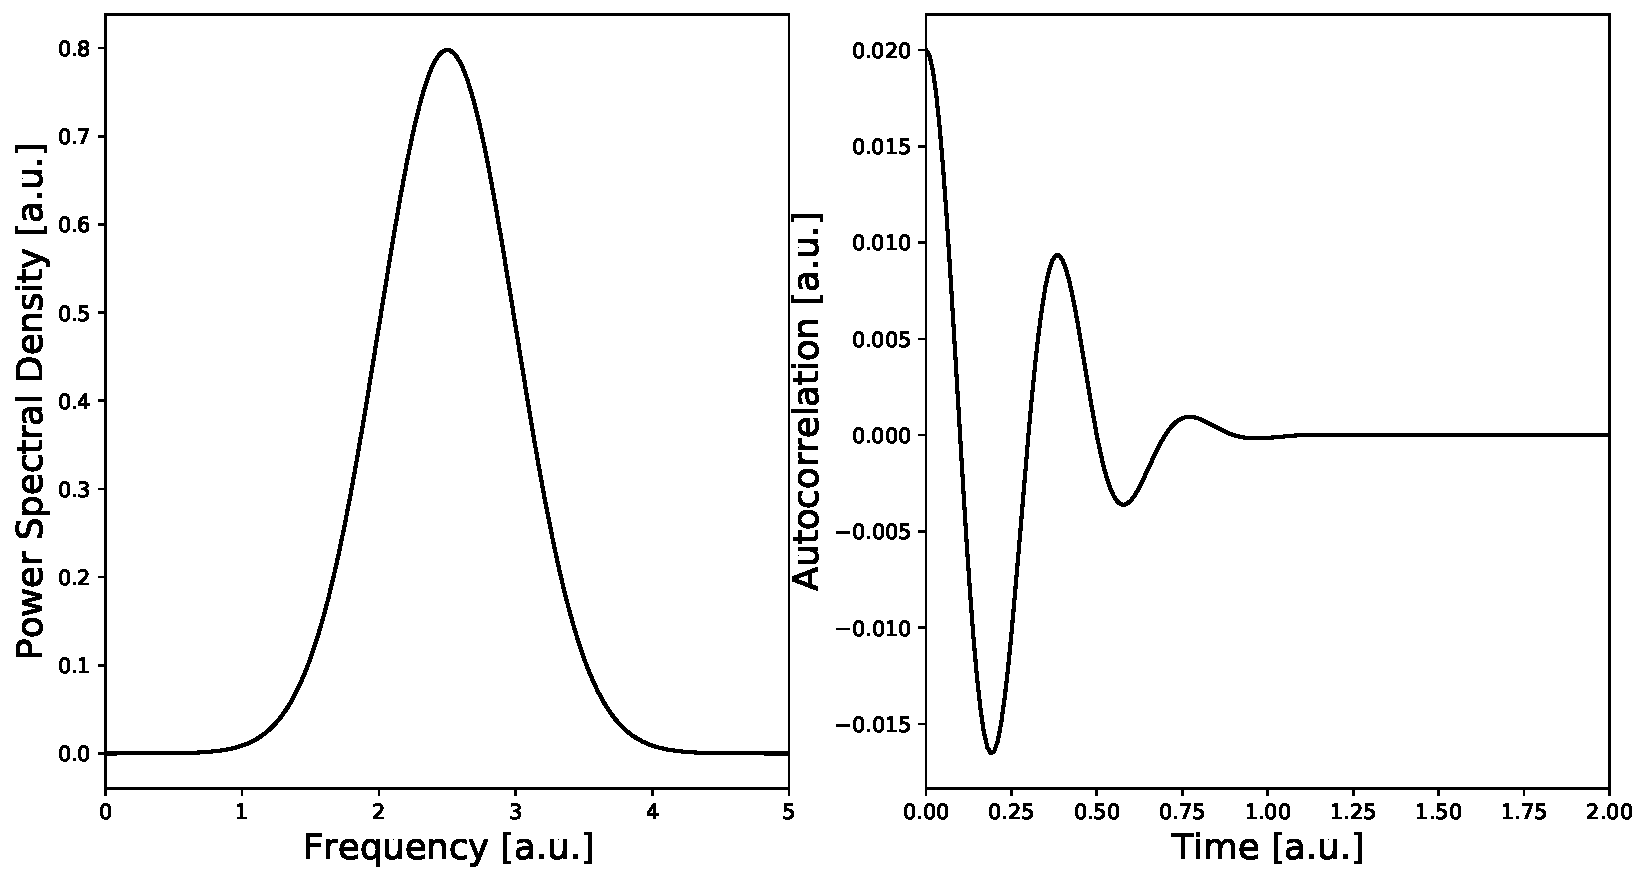
\includegraphics[width = \linewidth]{Images/Noise and PSD/NormalPSDautocorr.pdf}
        \caption{A priori spectrum (left) and autocorrelation (right)}
        \label{fig:autocorr}
\end{figure}and, since process has zero mean, autocovariance and autocorrelation matrices are identical. \\ 
Using the properties of Toeplitz matrices (see appendix \ref{app:Toeplitz}) and the relation between autocorrelation and power spectral density, it is immediate to verify that, in the limit of large number of time samples, the distribution of noise in frequency domain is given by:
\begin{equation}
    p(\tilde{n}(f_i) \vert I) \propto \exp{\left\{-\frac{1}{2}\sum_i\frac{n_i ^2}{S(f_i)}\right\}},
\end{equation}
so that the role of PSD appears to be clear: it is the diagonal covariance matrix for the noise distribution in Fourier Domain: \\
\begin{equation}
    \nonumber
    <\tilde n_i \tilde n_j > = S(f_i)\delta_{ij}.
\end{equation}
With this information, it is easy to generate any time series with power spectral density of any shape.
Choosing a priori values for sampling interval $dt$ and total time of observation $T$, recalling Nyquist theory of sampling, we generate arrays of given length N / 2 in frequency domain from 0 to the Nyquist Frequency $f_{Ny} = \frac{1}{2 dt}$. We then convert noise to the time domain using an Inverse Fast Fourier Transform.\cite{oliphant2006guide}\cite{van2011numpy} \\ Basic idea for fast algorithm used to construct noise can be found in ~\cite{noiseGen}. We worked it out in a slightly different way, the imaginary component is not obtained sampling a random complex phase from a uniform distribution. We choose to sample both real and imaginary part from two identical normal distribution distributing variance in a proper way between real and imaginary components. 
\section{Test on Time Series}
It is now possible to test the three methods on a given time series. We will concentrate on a power spectral density that is a normal distribution with mean $\mu = 2.5 \quad units$ and standard deviation $\sigma = 0.5 \quad units$.
We will apply Burg method with each optimizer on a large amount of simulated dataset, obtaining a variety of estimate for PSD. We will study statistical properties for both single reproductions and ensemble average. In many cases, such as gravitational waves, one cannot observe multiple time series realizations for a fixed process, so that single reproduction studies are probably more useful. Still, study of ensemble average is important to highlight some interesting properties. In this way we can fully characterize the performance of each optimizer 
We will attentively study the role of the filter length estimate M in determining the accuracy of the reconstruction. We will consider every optimizer separately and compare result only at the end of this section. We will then study in depth the Advanced LIGO design sensitivity power spectrum \cite{Ligo}
\subsection{Normal Power Spectral Density}
\begin{figure}
    \centering
        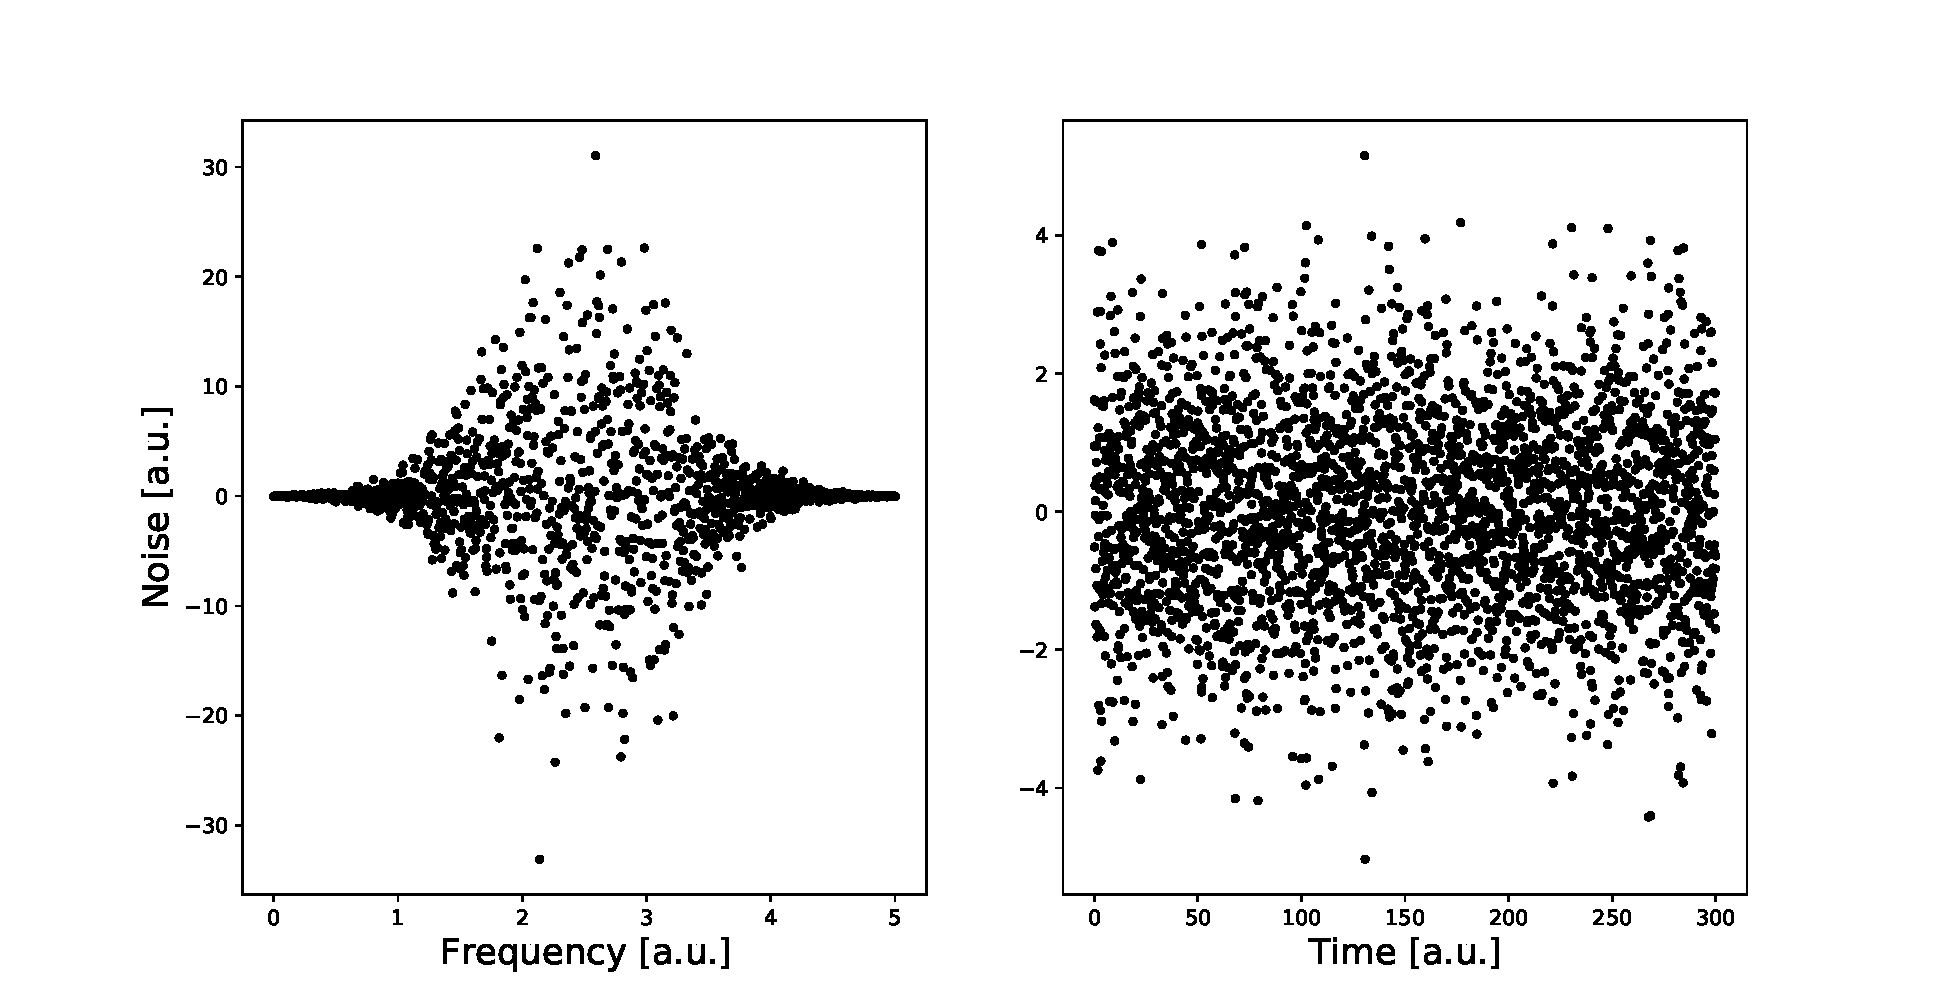
\includegraphics[scale = .43]{Images/NormalPSD/NormalNoise.pdf}
    \caption{Noise in both time and frequency domain. Frequency noise behaviour is representative of the chosen spectrum, having its maximum amplitude around $f = 2.5 au$}
    \label{fig:noise}
\end{figure}
Fig \ref{fig:noise} shows a realization of the gaussian process in the frequency (left panel) and time domain (right panel).   \\ 
To study noise with normal-shaped PSD, we generate 1000 datasets of 3000 points each. This will provide a number of samples that is large enough to perform statistical analysis. For every dataset we will reproduce its spectrum with every optimization method. We will show that the quality of reconstruction is very different in different parts of the spectrum: the minimum of the error will be achieved around the peaks, increasing fastly in the tails
 \\ \\ 
\subsubsection{Final Prediction Error (FPE)}
The estimate of the recursive order obtained with FPE on the 1000 realization of noise, is found to lay between 30 and 70. Qualitatively, there is a good agreement between the reconstructed spectrum and the true spectrum: a logarithmic plot of the mean of all the spectra versus the true spectrum is reported in \textbf{Figure \ref{fig:FPEmean}} with 90\% credible regions. It is evident that, despite not too large error bars, the tail of the normal distribution is not comprised in the interval of the estimation. 
\begin{figure}[H]
    \centering
    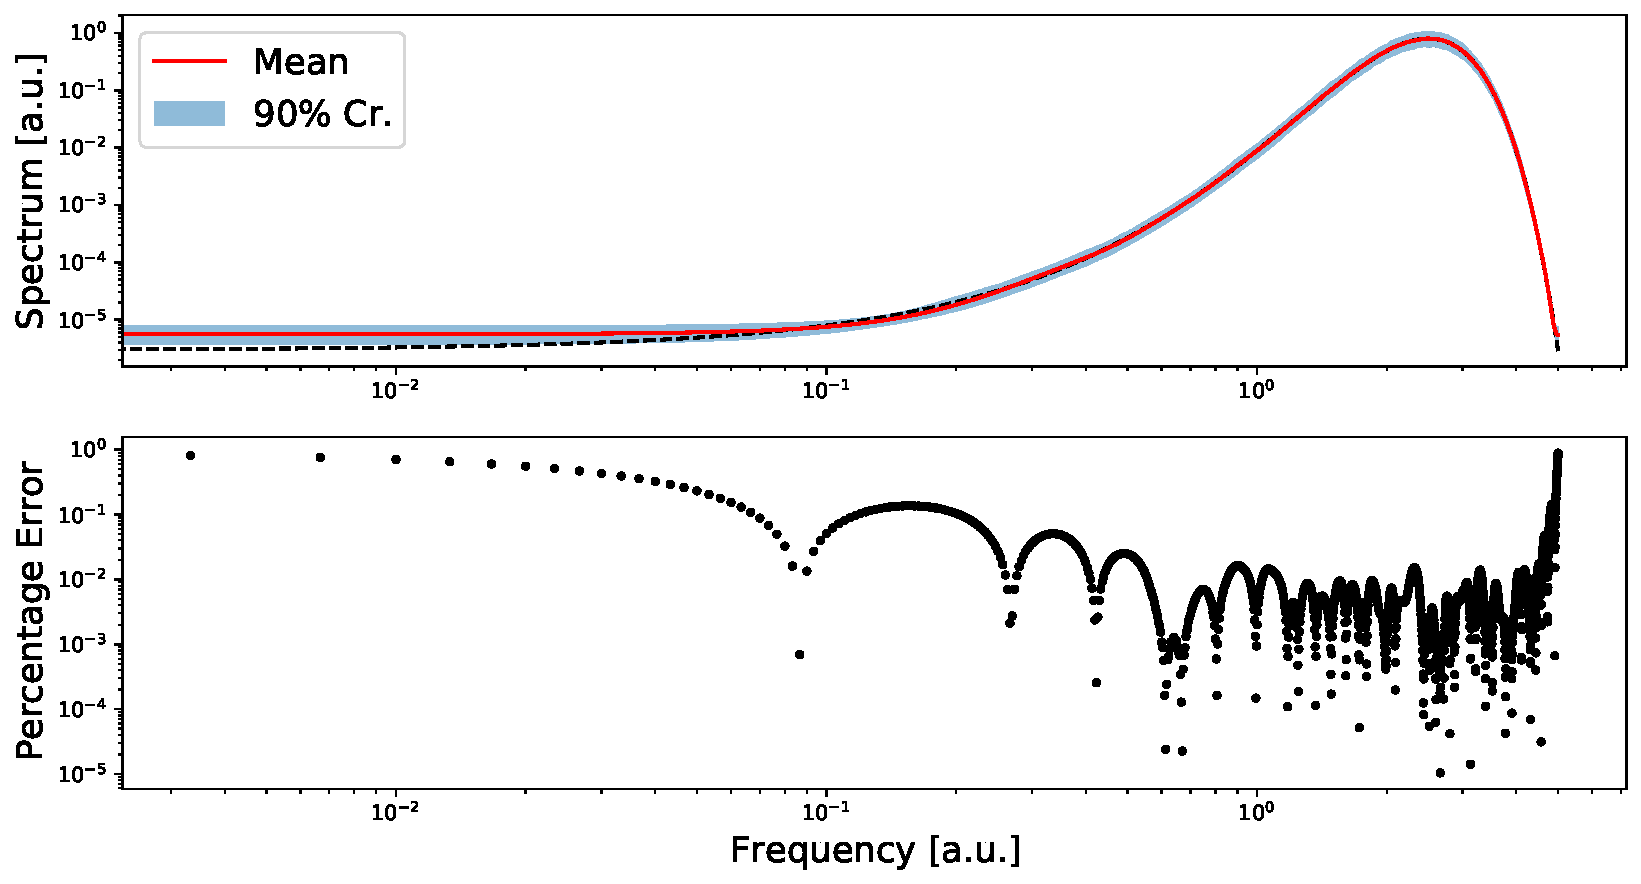
\includegraphics[scale = .4]{Images/NormalPSD/FPEpsdAndResiduals.pdf}
    \caption{Ensemble Average for FPE reconstruction with 90\% Credibility Regions (above) and percentage error (below)}
    \label{fig:FPEmean}
\end{figure}
To assess the magnitude of the disagreement, we compute the relative error between the mean spectrum $\hat{S}$ and the true spectrum $S$ for every frequency bin
\begin{equation}
    \nonumber
    r(f) = \frac{|\hat{S}(f) - S(f)|}{S(f)}\,.
\end{equation}
We found this to be a better choice than residuals since relative errors are not dependent on the magnitude of the data. Second Fig \ref{fig:FPEmean} (below) shows that the largest error in the reconstruction of the spectrum is in the tails, while in the bulk of the distribution we have a good approximation of the true function. 
For the entire spectrum, the mean relative error $\Bar{r}$ is 
\begin{equation}
    \nonumber
    \bar{r}_{\bar S, FPE} = 0.025.
\end{equation}
FPE performs well in reconstructing the spectrum even with relatively short time series, with a deviation from the true spectrum around 2\%, but it is evident that it is not able to capture all the features of the spectrum, since the reconstruction in the tails is inaccurate. If we compute the average percentage error in three standard deviations from the mean we gain an order of magnitude estimate of the accuracy of the reconstruction, obtaining: 
\begin{equation}
    \nonumber
    \bar{r}_{\bar S, FPE}^{\mu \pm 3\sigma} = 0.005. 
\end{equation}
and we can state the the method is highly performant in this frequency window. 
Since it is not always possible to work with more then one realization for a process, as in observational experiments, it is important to understand how this method behaves when we apply it on a single time series. In that case, the mean error and its standard deviation are: 
\begin{equation}
    \nonumber
    \bar r_{FPE} = 0.16; \quad \sigma_{r} = 0.16\,.
\end{equation}
The average error of a reconstruction based on a single time series is bigger than the one obtained considering the average of all the reconstructions.
Standard deviation of the errors assume small values and 90\% credibility regions (Cr.) in \ref{fig:FPEmean} are tight. This means that if we randomly take two of the reconstructed spectra, we expect their differences to be statistically small. These facts are evidence for FPE to be a relatively stable optimizer. 
We already said that the estimate for filter's length lays in a well defined range of values. The quality of the reconstruction, as noted in Chapter 1, depends on the order of the reconstructed AR process. 
To investigate this idea further, we plot the value of the optimizer for each recursion and the residuals as a function of the estimate for the order of the autoregressive process (\textbf{Figure \ref{fig:FPEErrorOrder}}),

\begin{figure}[H]
    \noindent
    \centering
    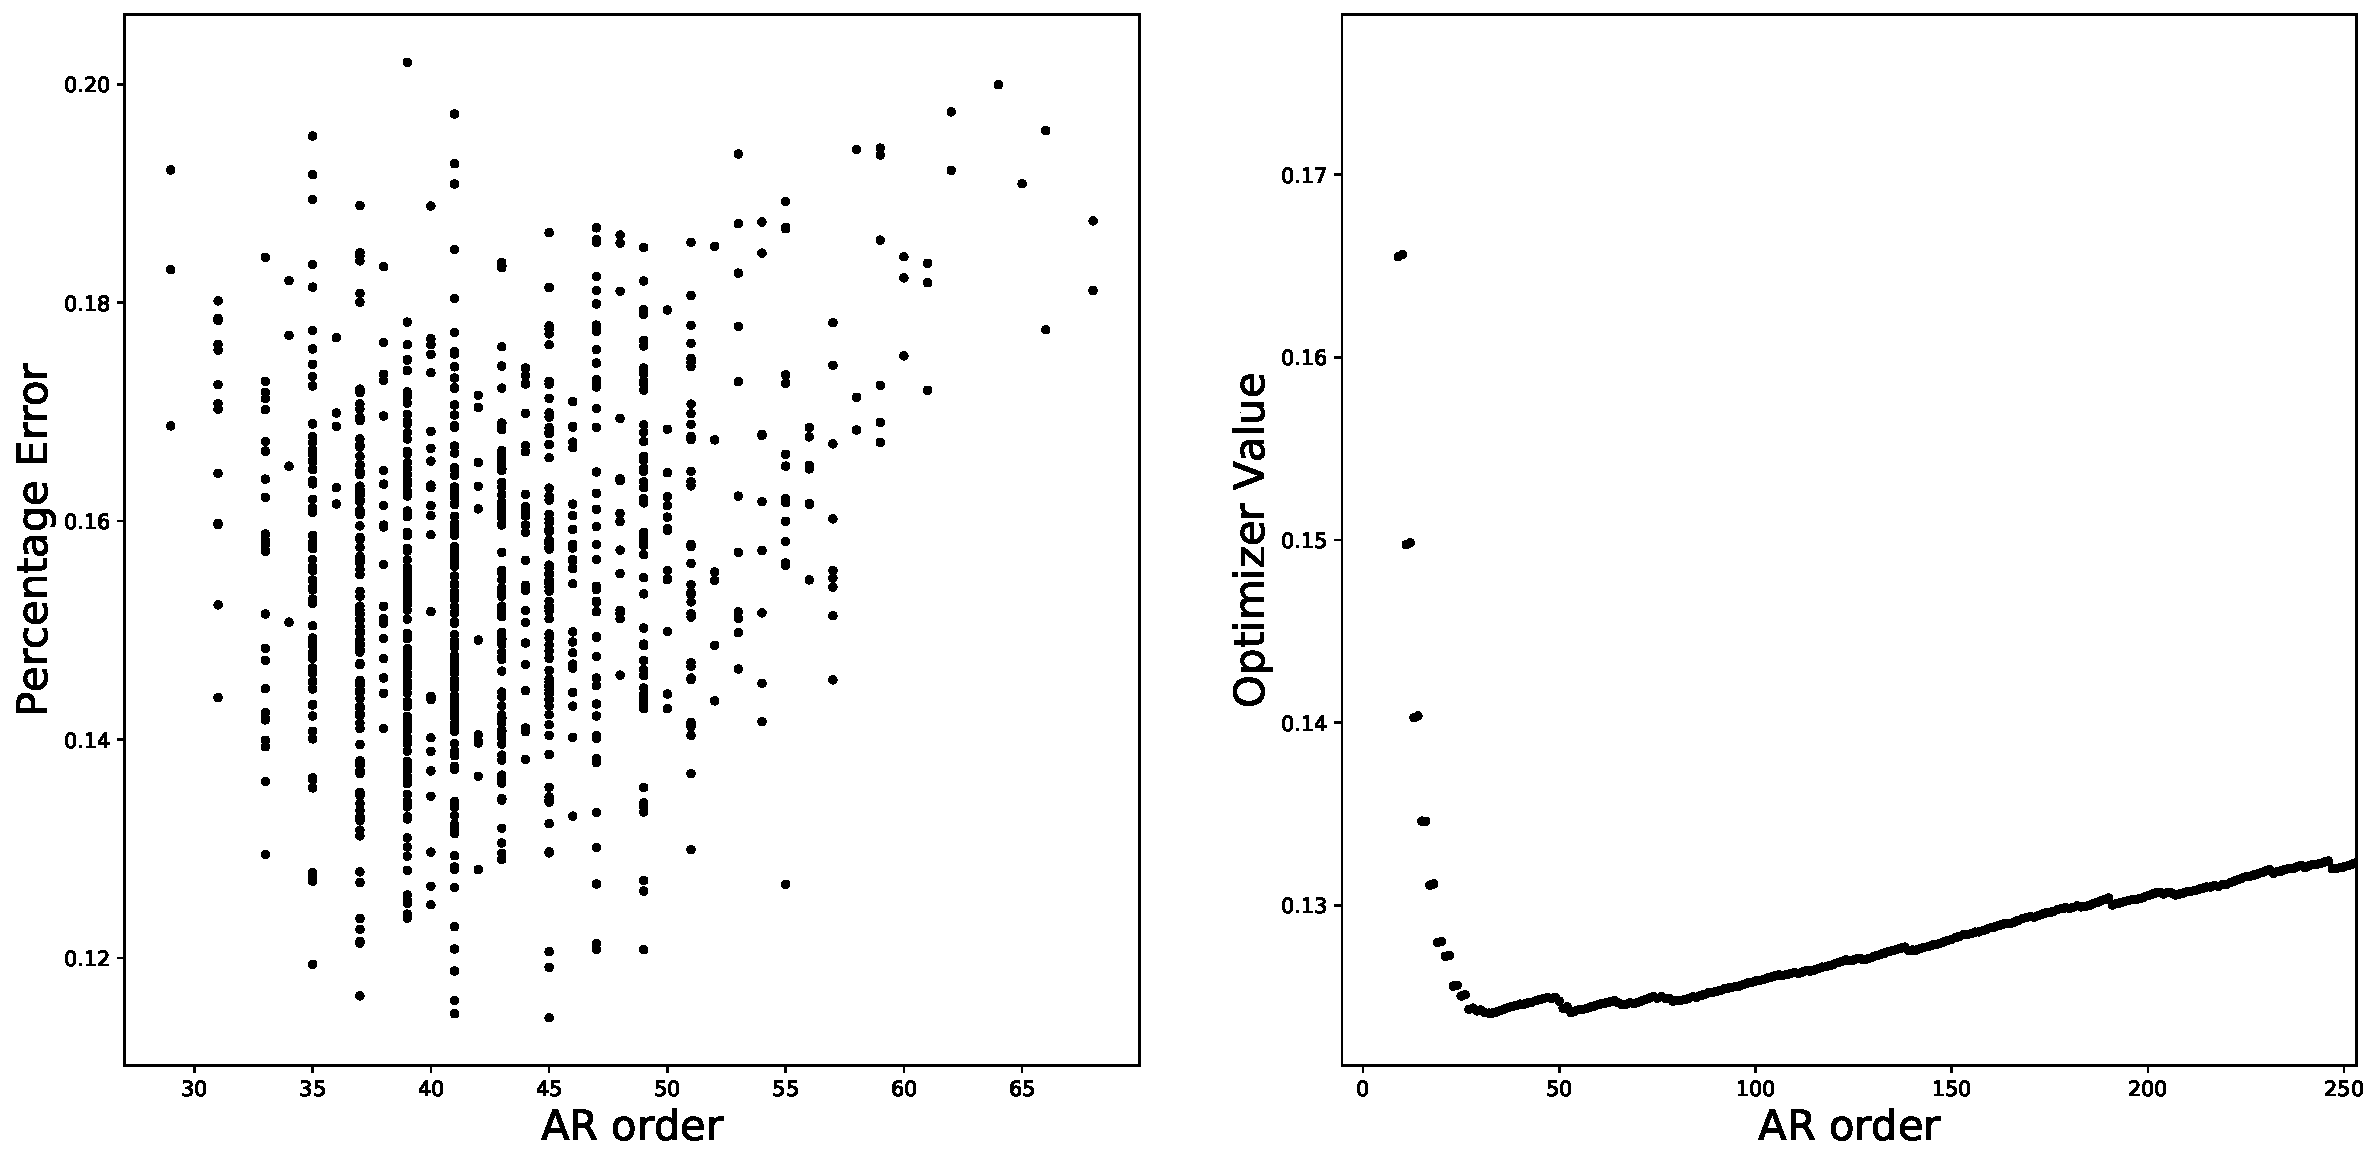
\includegraphics[scale = .3]{Images/NormalPSD/FPEoptimizer.pdf}
    \caption{Stability of FPE, that results in a cluster of values in a small region (left), is due to the typical behaviour of the optimizer as a function of the AR order (right).}
    \label{fig:FPEErrorOrder}
\end{figure}
Foremost evidence for the stability of this optimizer is found in its values as a function of the AR order. Figure \ref{fig:FPEErrorOrder} shows that Values tend to decrease monotonically until a sharp and well defined minimum is reached, to start growing again after this area. This is representative of the typical behaviour of this optimizer as a function of the length of the filter, and explains why the estimates for AR orders are confined in a small region. This plot also shows that most of the values collapsed in the region of AR orders comprised between 30 an 50. There are only few values outside this interval, and get fewer as order's estimate increases. In this region, there is no strong evidence of some correlation between the estimate for M and its associated relative error. It is important to notice that the estimate associated with the higher values of M (around $M > 60$) exhibit the highest 'mean' relative error. \\ 
We conclude that the FPE shows good quality reconstruction for the spectrum and very desirable stability properties, its estimate for filter's length M is clustered in a region where there is no dependence of error from M. 
\subsubsection{Optimum Bayes Decision Rule (OBD)}
The second optimizer in consideration is OBD.  (\textbf{Figure \ref{fig:OBD3000}}) shows a good agreement between the average over the reconstructions and true spectrum.
\begin{figure}[H]
    \centering
    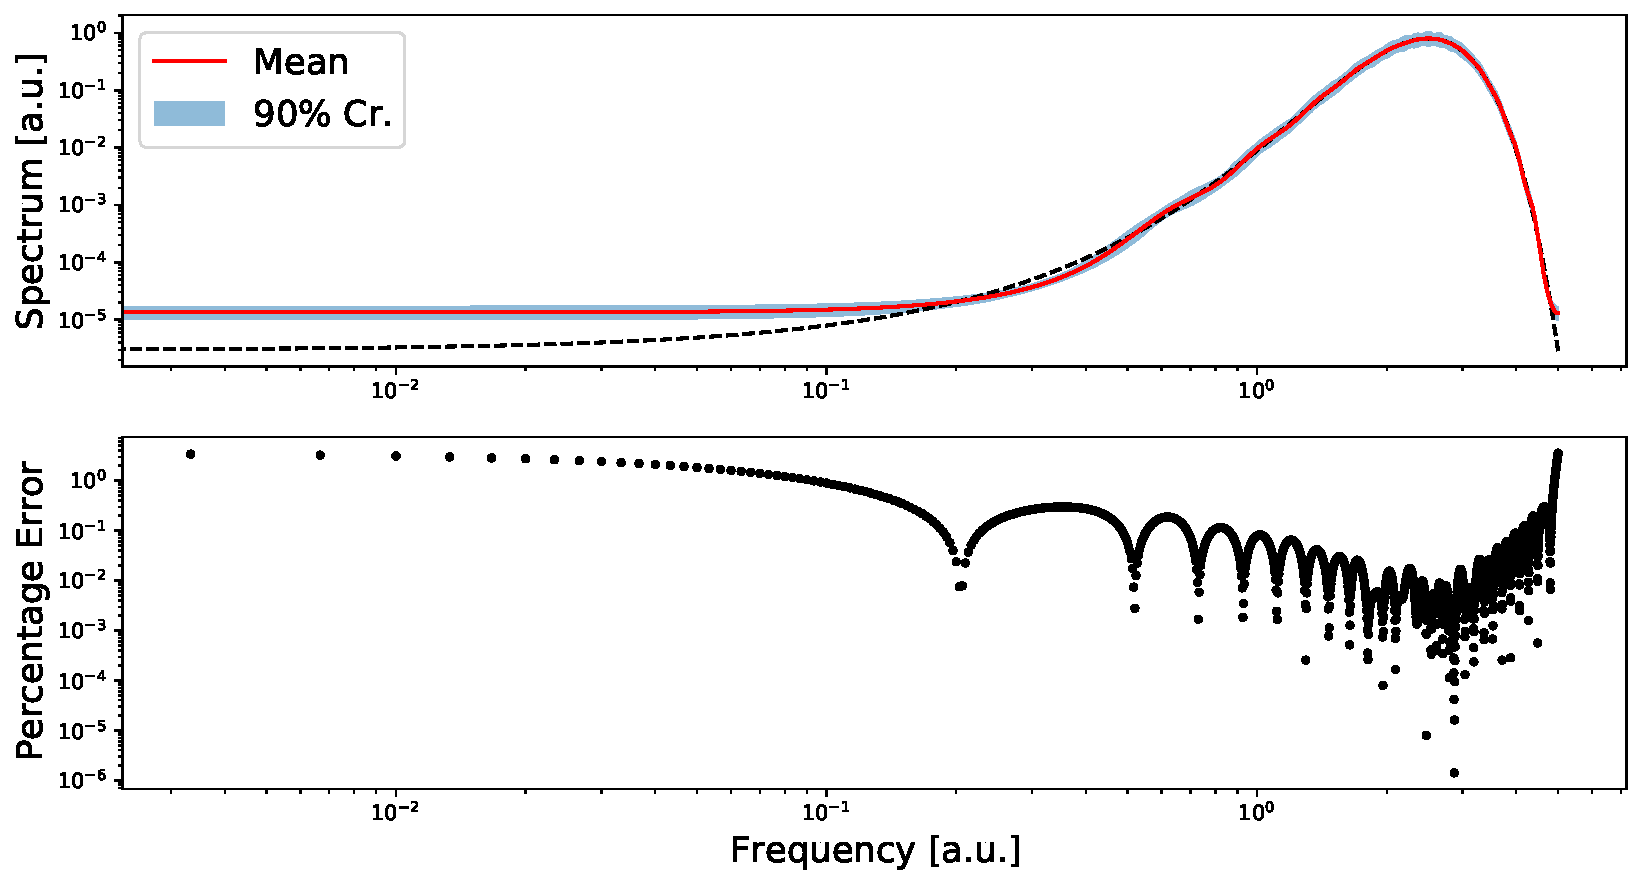
\includegraphics[scale = .45]{Images/NormalPSD/OBDpsdAndResiduals.pdf}
    \caption{Reconstruction of the spectrum from 1000 simulations with OBD optimizer. Plot is mean of all the results with 90\% credibility regions (above) and percentage error (below)}
    \label{fig:OBD3000}
\end{figure}
The same behaviour of FPE is observed, a good quality reconstruction at the center of the distribution with quite small Credibility regions (Cr.) at a $90$\% credibility level.
Qualitatively they behave similarly but quantitatively the disagreement of this method is found to be even larger than the one obtained with FPE, as can be noticed in the plot of relative errors in figure \ref{fig:OBD3000} (below) where at the extremes the inaccuracy is even larger than 300\% with respect to the real value of the spectrum. For the overall spectrum and within three standard deviation from the mean, we find that the reconstructed spectrum has a deviation of
\begin{equation}
    \nonumber
    r_{\bar S, OBD} = 0.15, \qquad r^{\mu \pm 3\sigma}_{\bar S, OBD} = 0.018. 
\end{equation}
When applied to single realizations of the time series, we find
\begin{equation}
    \nonumber
    \bar{r}_{OBD} = 0.237, \qquad \sigma_{r, OBD} = 0.0296.
\end{equation}
It is interesting to notice that overall relative error of the average spectrum is of the same order of magnitude of the average single reconstruction for the spectrum. Averaging over a 1000 realisations does not substantially improve our results. As a function of the filter length, the values taken by the OBD cluster in a small region, indicating the stability of the reconstructed process order $M$.

\begin{figure}[H]
    \centering
    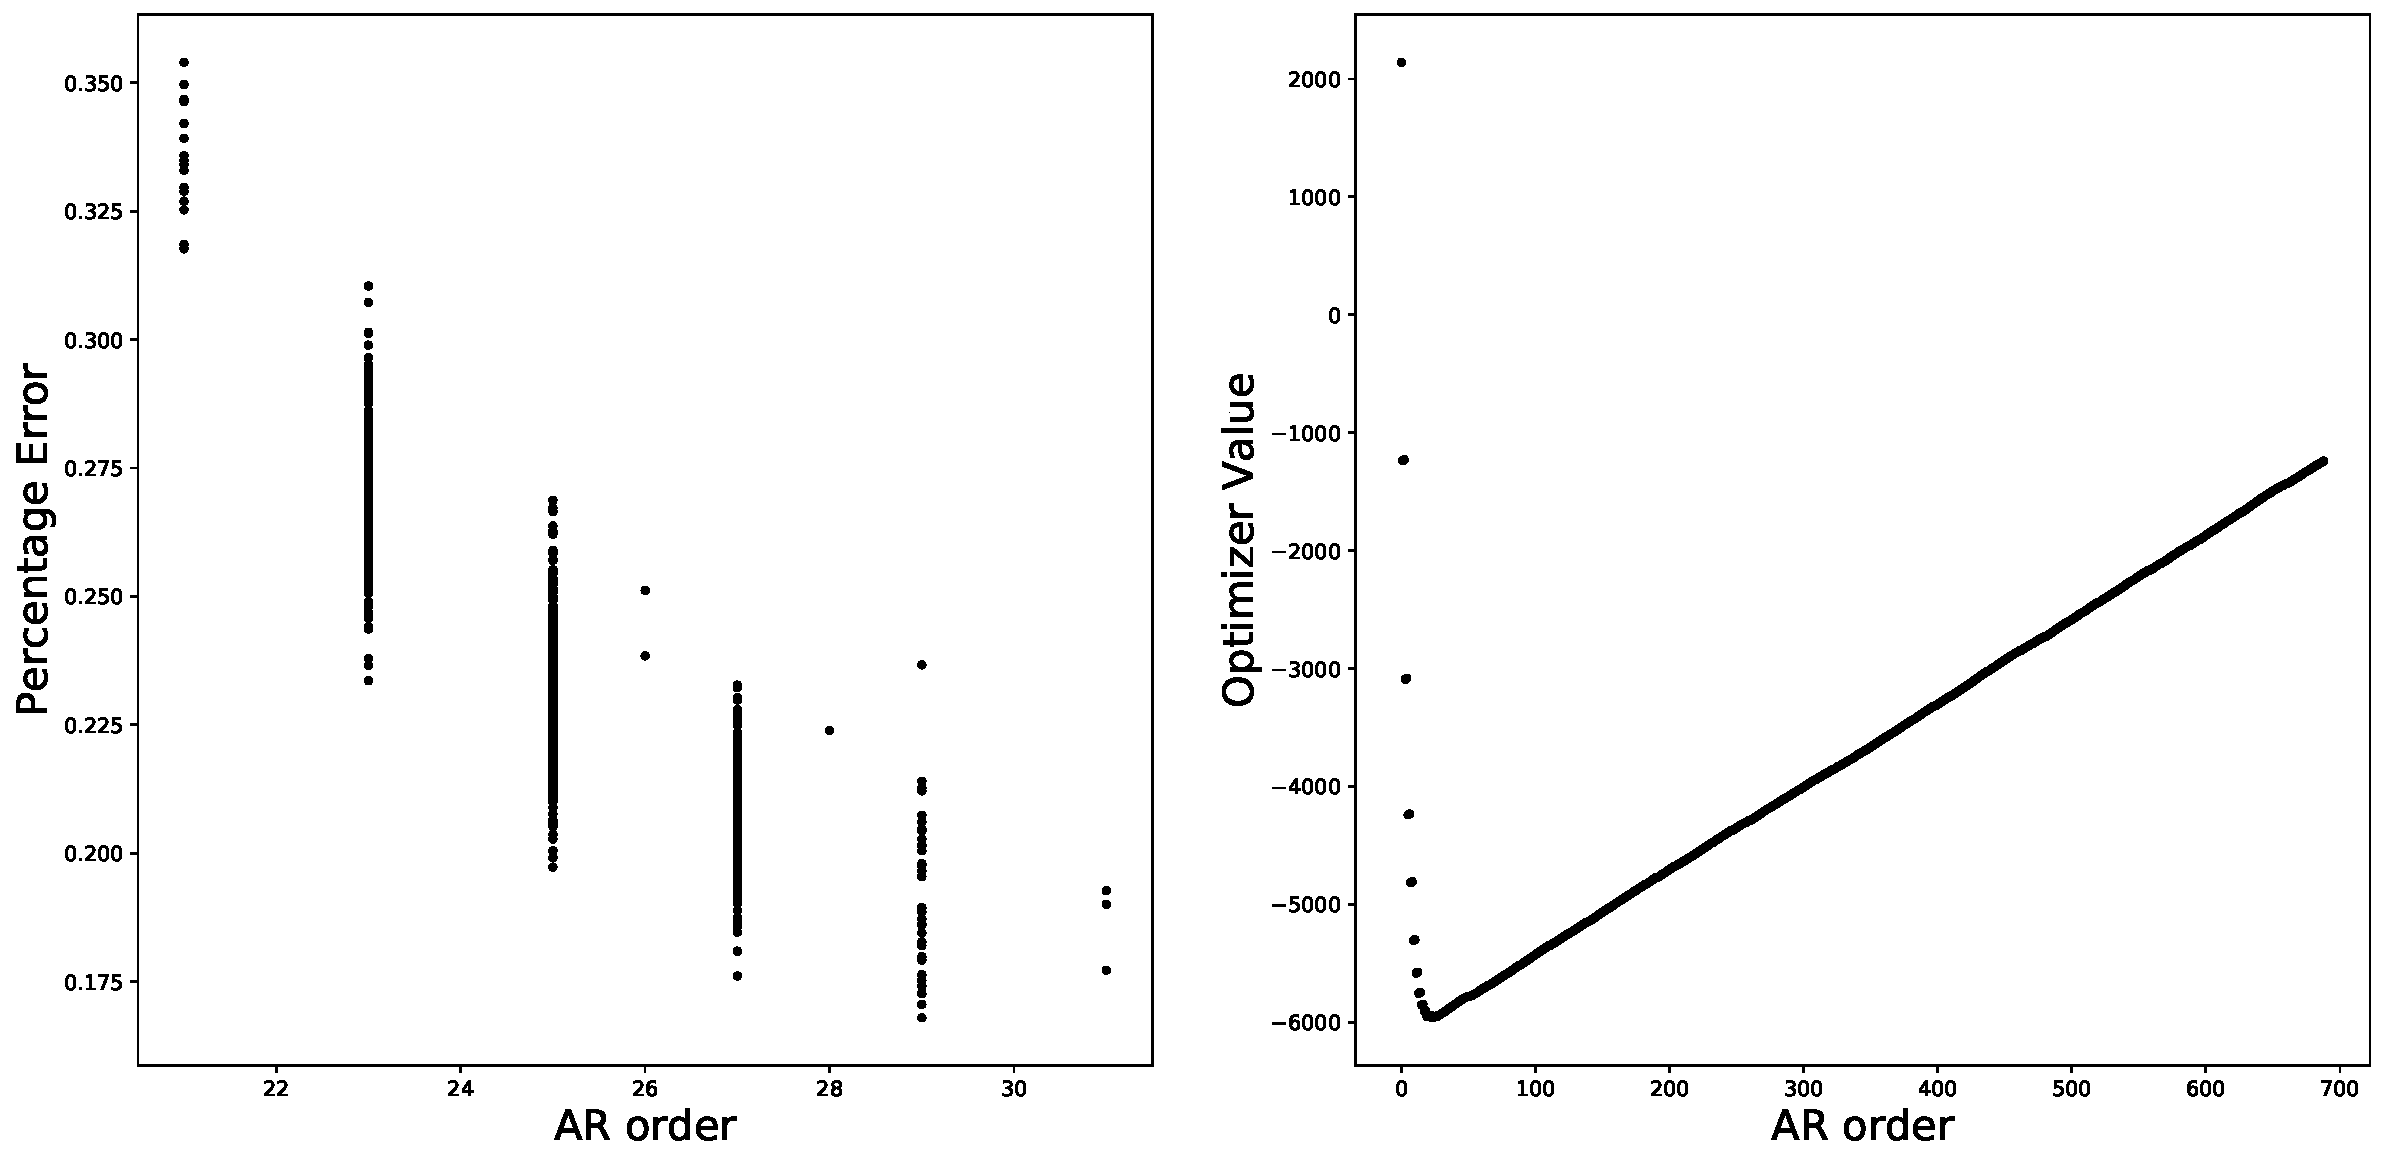
\includegraphics[scale = .3]{Images/NormalPSD/OBDoptimizer.pdf}
    \caption{Stability of OBD, that results in a cluster of values in a small region (left), is due to the typical behaviour of the optimizer as a function of the AR order (right)}
       \label{fig:OBDErrorOrder}
\end{figure}we see that again our results are clustered in a very small region, due to the behaviour of the optimizer that converge in a small area before growing again. The estimate of the length of the filter is around $p = 20 \div 30$.Note the difference compared to FPE (see \ref{fig:FPEErrorOrder}); for OBD the mean relative error depends on $M$ as
\begin{equation}
    \hat r \sim M ^ {-2.016 \pm 0.006}.
\end{equation}
In summary, OBD shows greater error wherever in the spectrum, due to the fact that it choose filters that are too short and in a region where quality drastically change when changing M. In this case we can say that we have a stable estimate for M, but due to this dependence, the estimate is not as stable as FPE's. 
\subsubsection{Criterion Autoregressive Transfer function (CAT)}
This last criterion differs substantially from the two other optimizers. Figure \ref{fig:CATmean} (above) shows a good agreement between the estimate of the spectrum for every frequency
\begin{figure}[H]
    \centering
    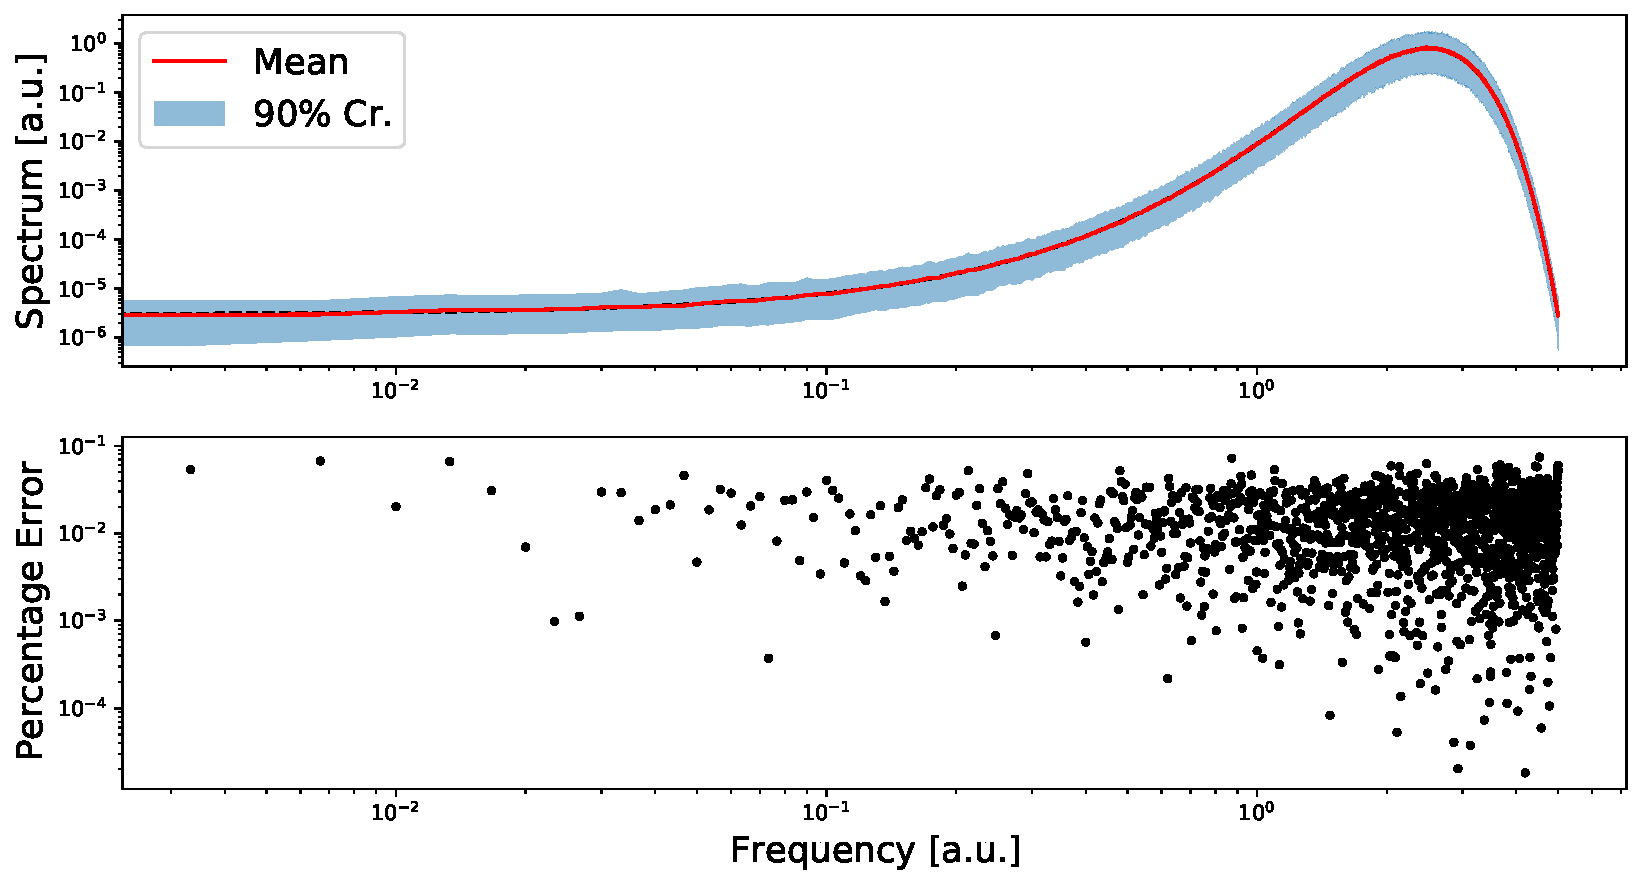
\includegraphics[scale = .43]{Images/CAT/CATnormal.pdf}
    \caption{Mean spectrum for CAT optimizer, 1000 simulations for 3000 points datasets}
    \label{fig:CATmean}
\end{figure} and also tails are well captured by the average spectrum. However, the variance of the reconstructed spectrum is quite large, much larger than for FPE and OBD. In general, the relative error is nearly constant, $\sim 10\%$ over all frequencies, see  Fig. \ref{fig:CATmean} (below). The residuals, averaged over all frequencies, are: 
\begin{equation}
    \nonumber
    \bar r_{\bar S, CAT} = 0.016 \qquad \bar r^{\mu \pm \sigma}_{\bar S, CAT} = 0.017.
\end{equation}
the overall reconstruction is thus quite accurate, with deviations from the simulated spectrum of the order of $1\% \div 2\%$.\\
The picture drastically changes in the case of individual time series realizations. The average residuals are, in fact
\begin{equation}
    \bar r_{CAT} = 0.42 \qquad \sigma_{CAT} = .44\,.
\end{equation}
The error is indeed $\sim 42\%$, hence much larger than in the case of FPE and OBD. Both large error bars and the large standard deviation are indications of the instability of this optimizer. This is exemplified by the variety of different spectra that can be obtained considering different time series. 

\begin{figure}[H]
    \centering
    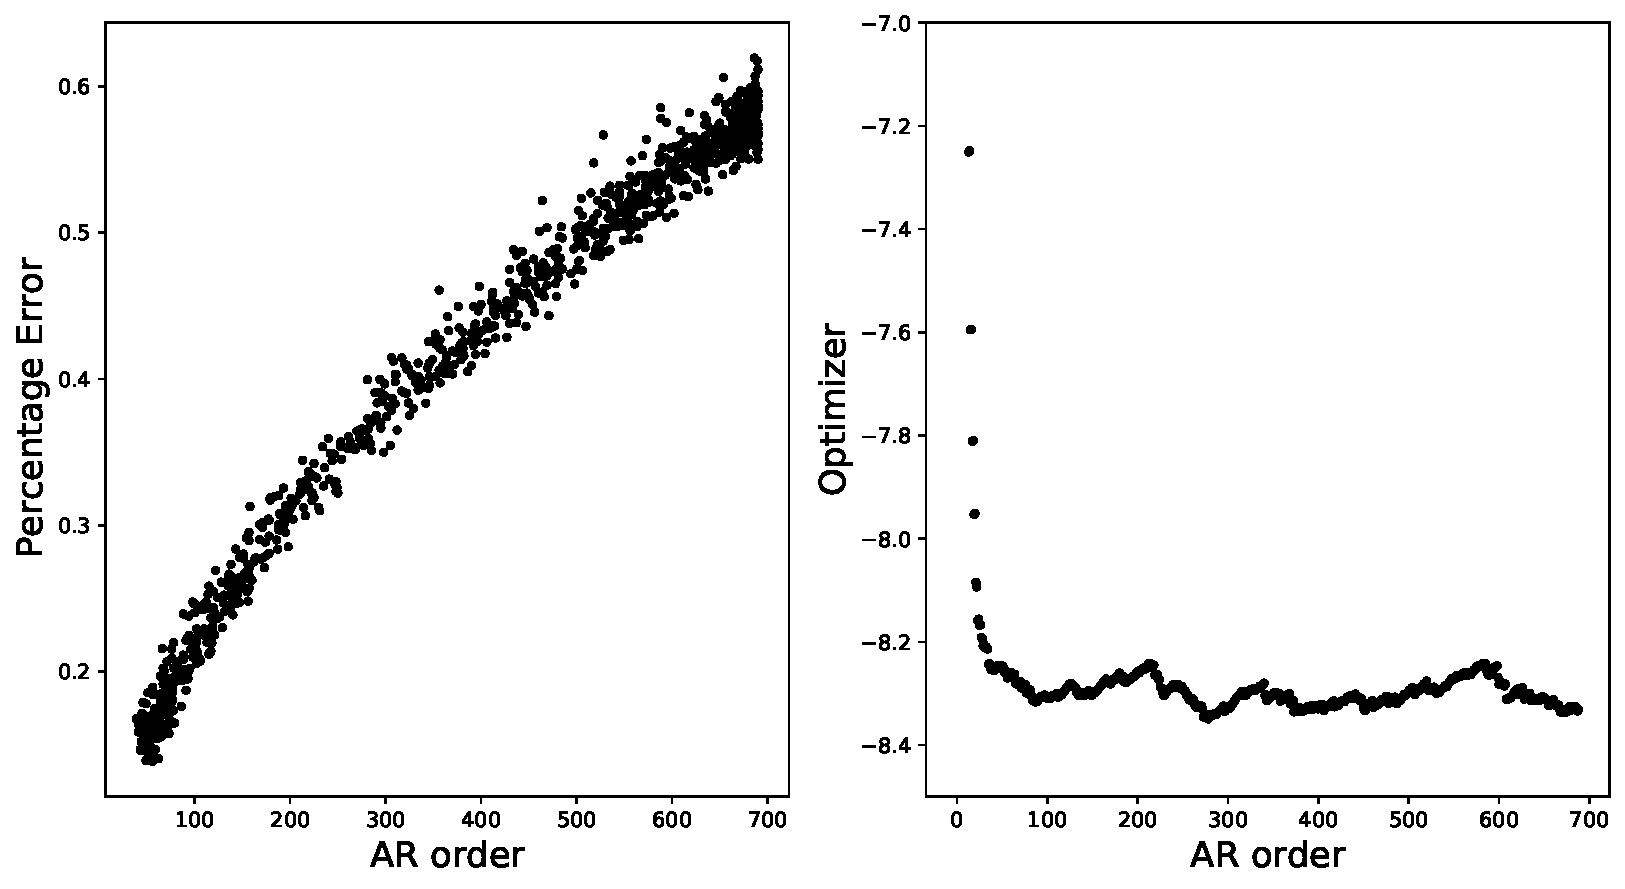
\includegraphics[scale = .43]{Images/CAT/CAToptimizer1.pdf}
    \caption{CAT is not a stable optimizer since its optimizer do not converge to any specific region of the AR estimate order}
    \label{fig:CAToptimizer}

\end{figure}
The reason for this behaviour, can be found in \textbf{Figure (\ref{fig:CAToptimizer})}. CAT does not converge to any specific value for the order of the autoregressive process. In turn, this results in estimates for the order that span a large range.  Figure \ref{fig:CAToptimizer} also shows a strong dependence of the error on the estimated length of the filter. The good quality of the reconstruction from the average spectrum can be explained as follows: long filters are able to capture features that short filters cannot see, like the big excursion in the size of datas of a normal distribution, but this length is also responsible of an augmented variance in the estimate, introducing spurious peaks in the reproduction (Figure \ref{fig:GaussMedian})

Averaging, the noise in each spectrum is cancelled. It is interesting that the cancelling of errors in averaging is property of gaussian noise (the process is gaussian, after all). This implies, in a sense, that each estimate of the spectrum is independent of any other, as suggested by the huge variance in the residuals. This instability is not a good property for an estimation, so that this estimator might be found to be optimal for repeatable experiments and not for single observation of some process. Another approach to this method will be proposed in section \ref{sec:ACAT}

\begin{figure}
    \centering
    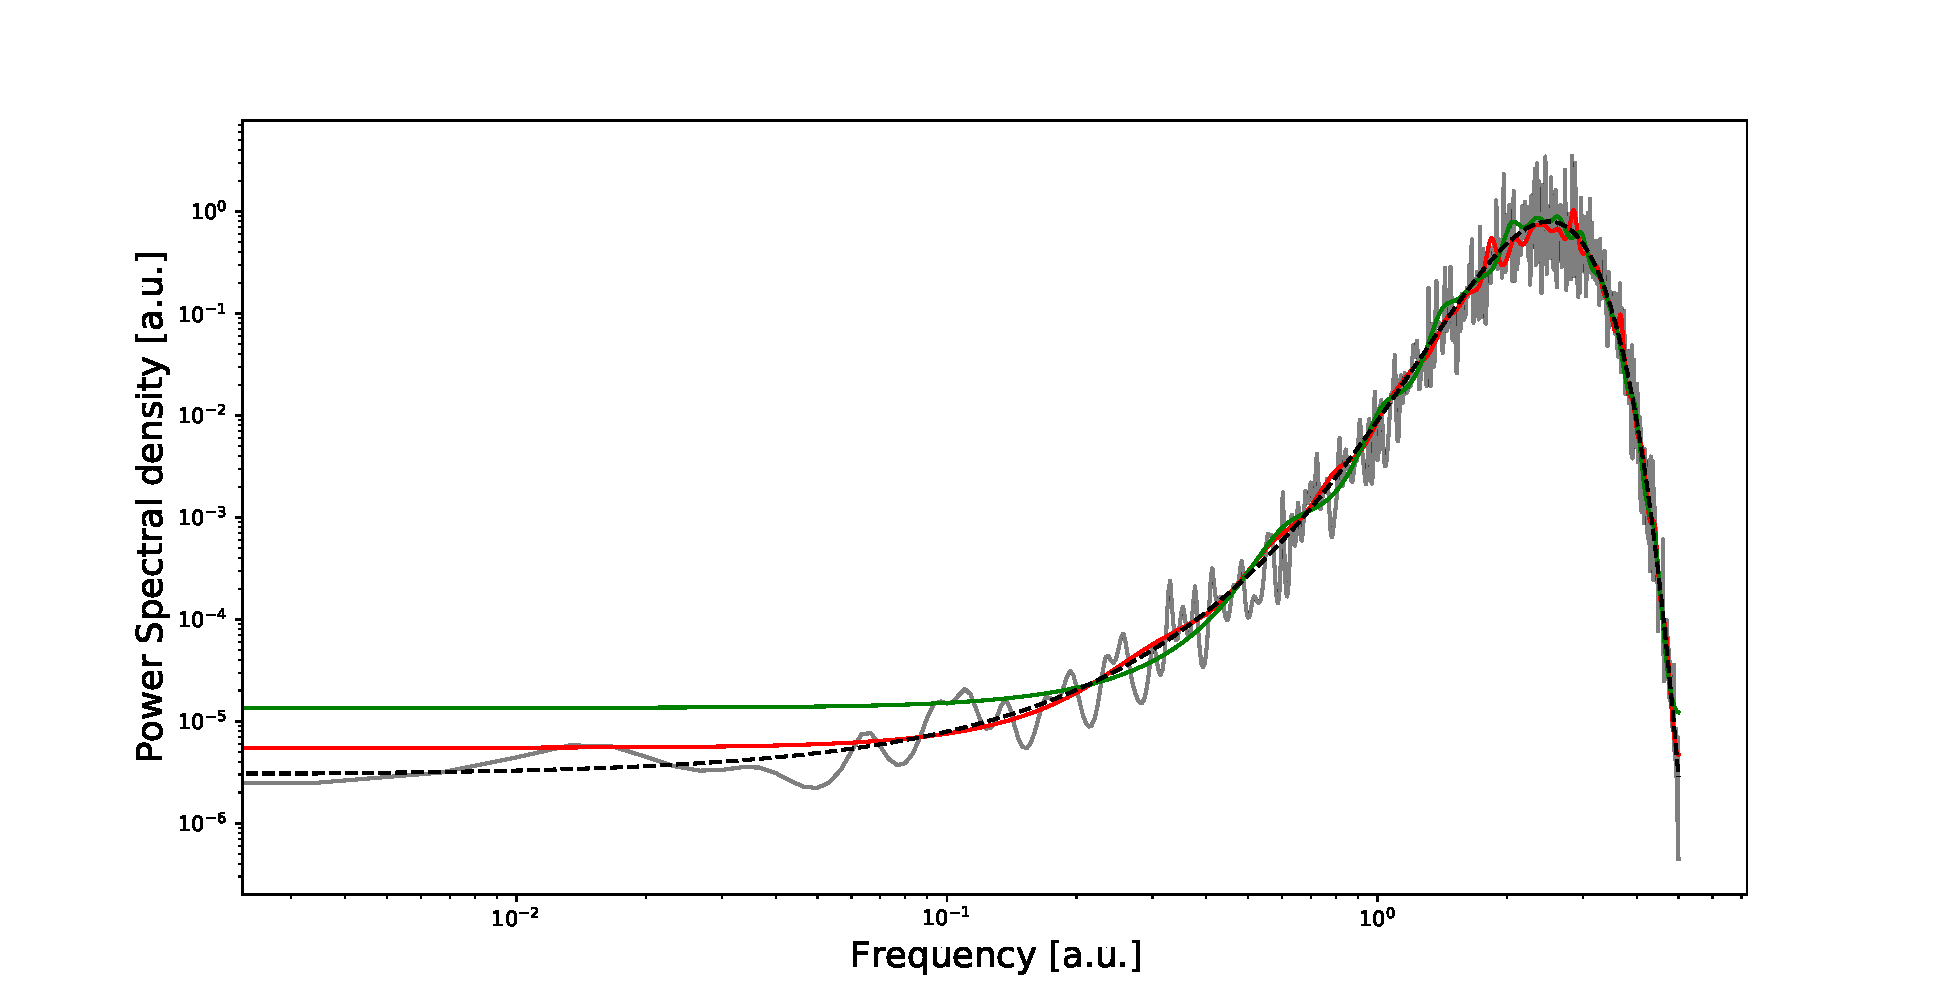
\includegraphics[scale = .45]{Images/NormalPSD/Gaussmedian.pdf}
    \caption{Reconstructed power spectral density with the three method. The reported reconstruction is the one that shows the median percentage error (overall)}
    \label{fig:GaussMedian}
\end{figure}
\subsection{Summary and Comparison}
\begin{figure}
    \centering
    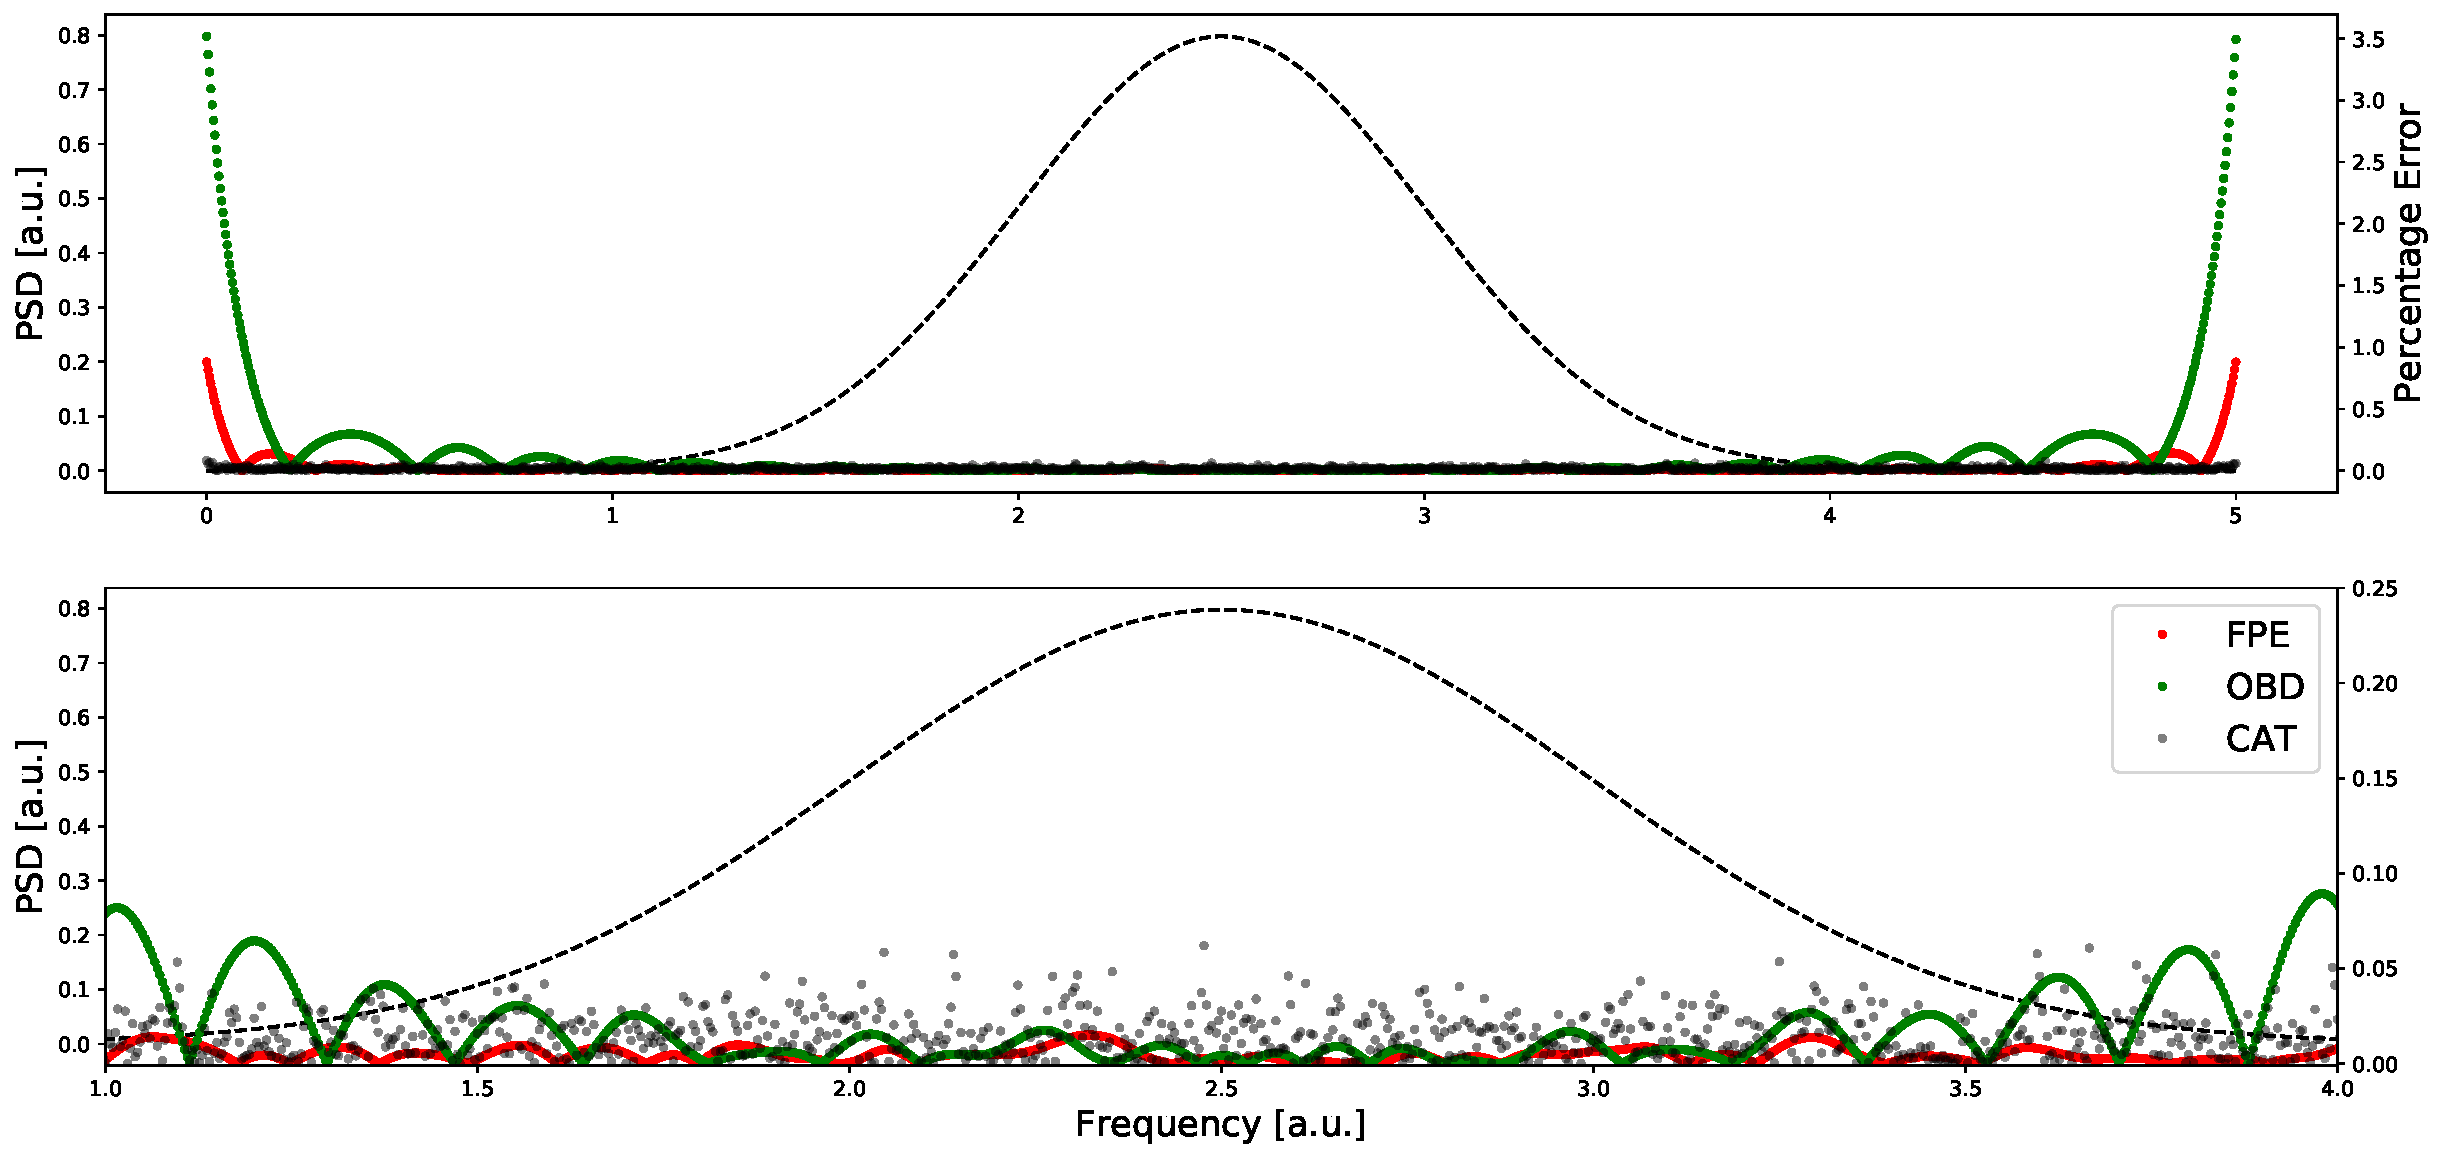
\includegraphics[scale = .3]{Images/NormalPSD/Normal Residuals.pdf}
    \caption{Percentage error in the reconstruction for every optimizer, as a function of the frequency. Lower panel restricts the domain to three standard deviation to increase the definition}
    \label{fig:NormalEnsembleResiduals}
\end{figure}
In our analysis, FPE and OBD optimizers are found to behave similarly while CAT shows completely different properties. Studying the average spectrum is not sufficient to choose which method behaves better. \\ 
The bad behaviour in the reconstruction of the tails from OBD and FPE might be due to the fact that very small values require longer filters. 
In fact when we consider the average for all the spectra we note that the shorter the filter the larger the error in the tails: OBD, which select the shortest filters, arrives to a $300 \%$ error at the extrema of the power spectral density, FPE which select intermediate order has got a $85\%$ error in same window, while CAT, that selects a wide range of long filters, has got a constant accuracy everywhere in the spectrum.  \\ 
Figure \ref{fig:NormalEnsembleResiduals} shows that CAT is the method that minimizes errors in the tails (upper plot), but if one restrict to three standard deviations from the mean, FPE is found to reach best accuracy (lower plot). 
The frequency averaged percentage error is reflecting this behaviour. Considering the whole reproduction, error's average and standard deviation are found to be: 
\begin{align*}
\centering
&r_{\bar S, FPE} = 0.025; \quad \sigma_{\bar S, FPE} = 0.083;  \\
&r_{\bar S, OBD} = 0.15;\quad \sigma_{\bar S, OBD} = 0.42 ; \\ 
&r_{\bar S, CAT} = 0.015; \quad \sigma_{\bar S, CAT} = 0.012
\end{align*}
In is interesting to see that the average for FPE and OBD is strongly affected from the high value of the error in the tails of the distribution. If one consider the three standard deviations from the mean, the value of the error substantially decreases, 
\begin{align*}
\centering
&r_{\bar S, FPE} = 0.005; \quad \sigma_{\bar S, FPE} = 0.004;  \\
&r_{\bar S, OBD} = 0.018;\quad \sigma_{\bar S, OBD} = 0.019 ; \\ 
&r_{\bar S, CAT} = 0.015; \quad \sigma_{\bar S, CAT} = 0.011
\end{align*}
showing that the overall percentage error is just a first indicator for the quality of the reproduction, but is not sufficient to perform a full characterization. \\
It is evident that tails do not affect CAT  average error and standard deviation at all, so that it's accuracy is approximately constant everywhere in the spectrum. \\ \ 
Since both FPE and CAT shows pros and cons, at this level, there is no reason to choose between them.\\ 
Analyzing the resolution of the single reconstruction, figure \ref{fig:optcomparison} clearly shows that FPE minimize overall relative error giving a stable result.\\ 
CAT instead shows a larger error and do not converge to any specific value. Almost every reproduction obtained with CAT is worst with respect to those obtained with FPE, but their mean is more precise. \\ 
It's instability is probably the cause for this behaviour. Since it does not show a strong convergence to some order with respect to others, very different lengths are selected.
Longer lengths are able to capture a lot of details but are more likely to introduce noise. In other words, long filters reduce bias but increment the variance of the result. 
Taking the average, for central limit theorem the error decreases as $\sim \frac{1}{\sqrt{N}}$. In this way we compensate noise and obtain a spectrum with small bias and small fluctuations.
Considering the average, CAT reconstruct precisely and with good accuracy every part of the spectrum, even if in "regular" parts best accuracy is reached from FPE. For a single reproduction, CAT is very noisy and unstable, while FPE performs the better. \ref{fig:optcomparison}
\begin{figure}
    \centering
    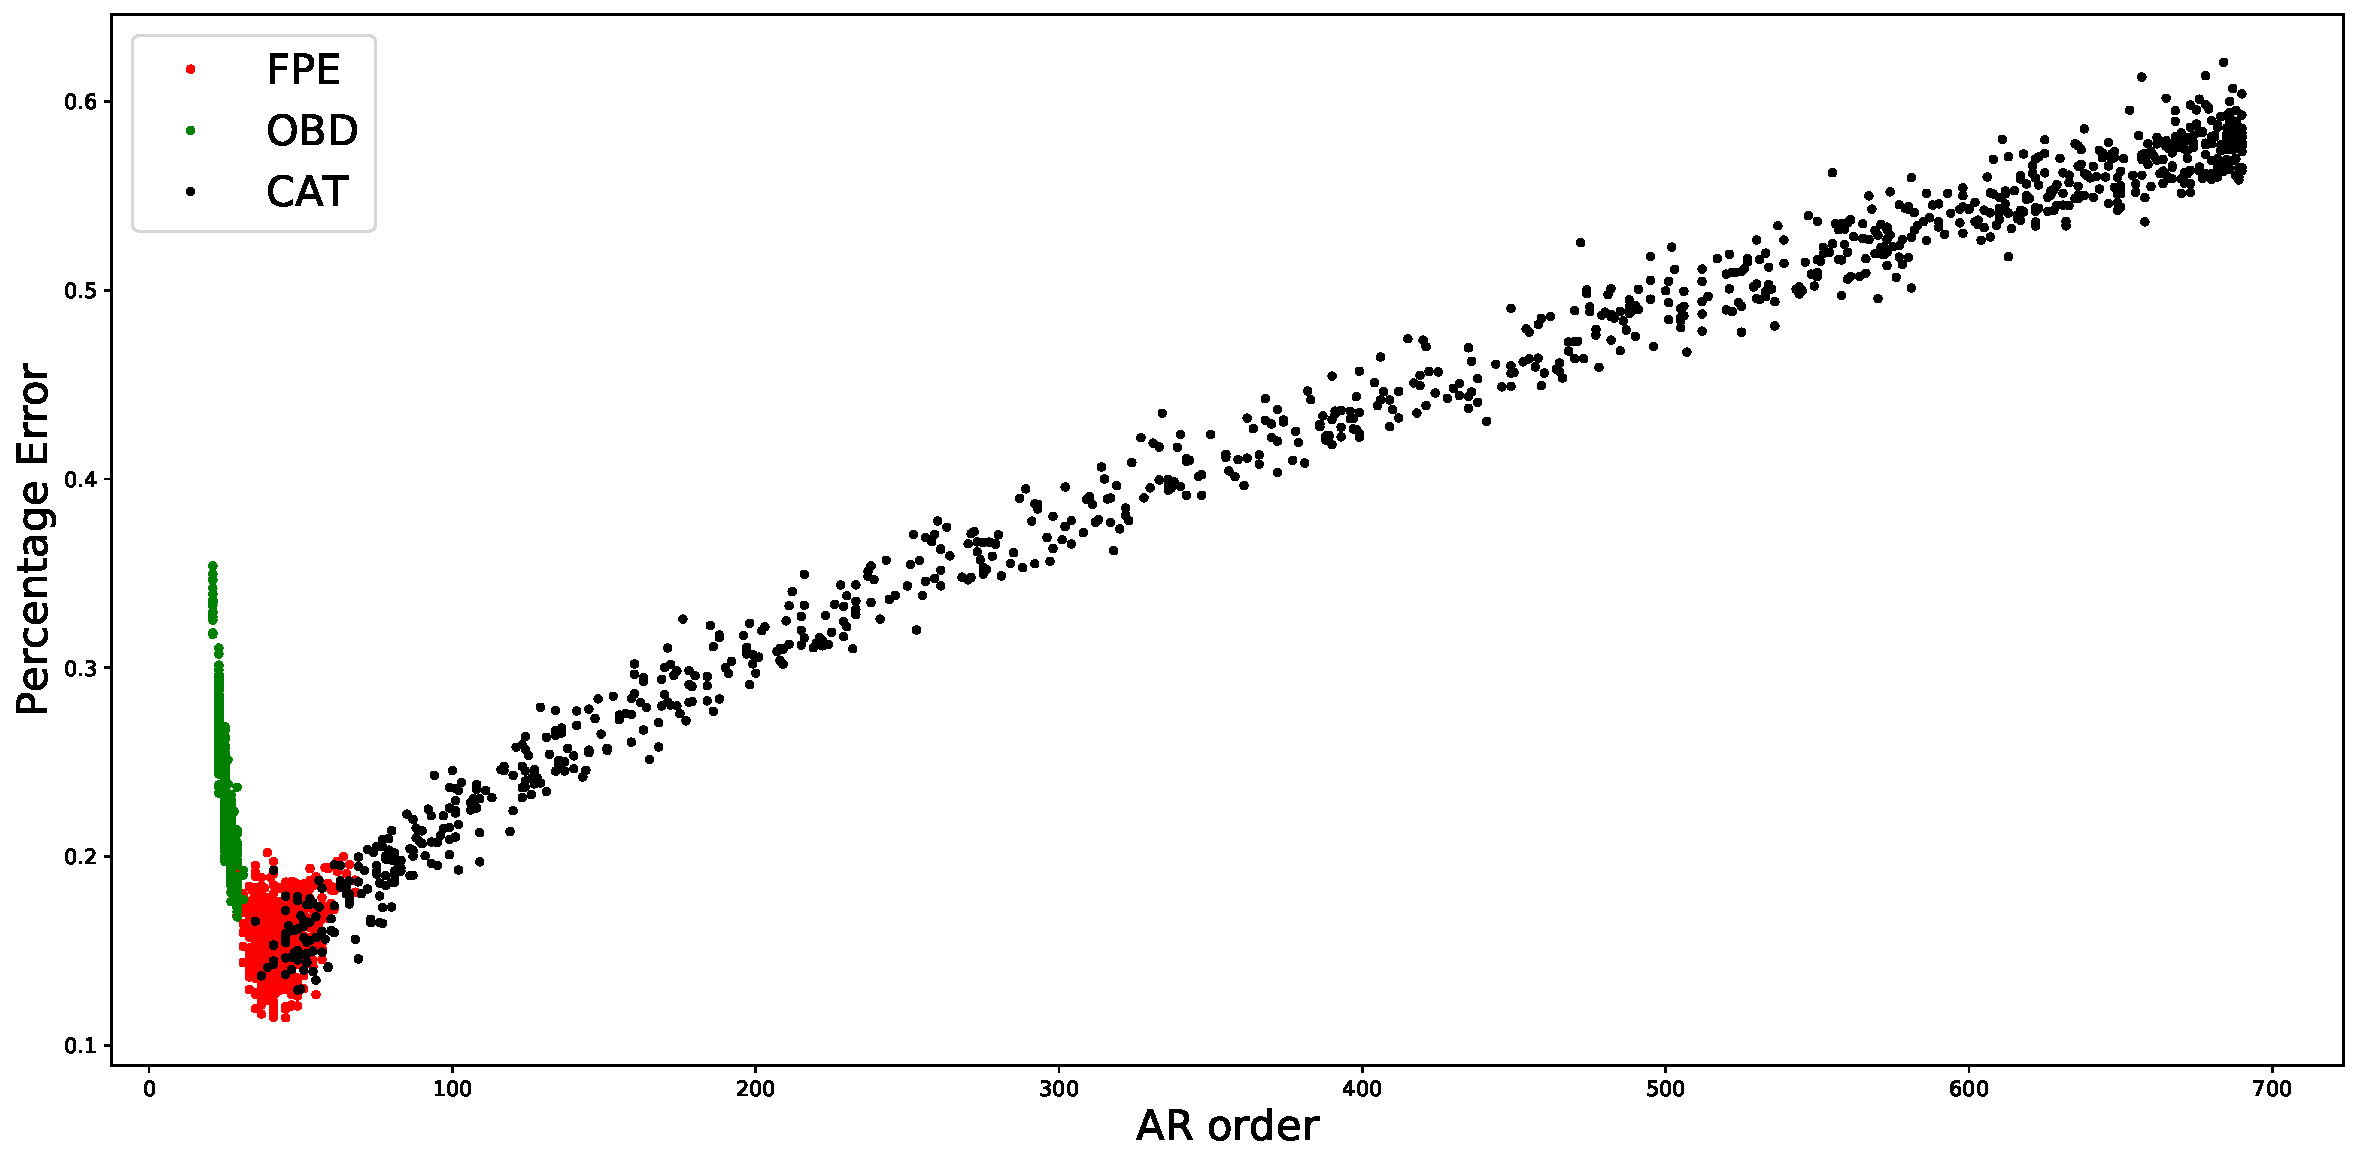
\includegraphics[scale = .3]{Images/NormalPSD/NormalPSDcomparison.pdf}
    \caption{Relative error as function of the length of the filter.}
    \label{fig:optcomparison}
\end{figure}
\begin{figure}
    \hfill
    \centering
    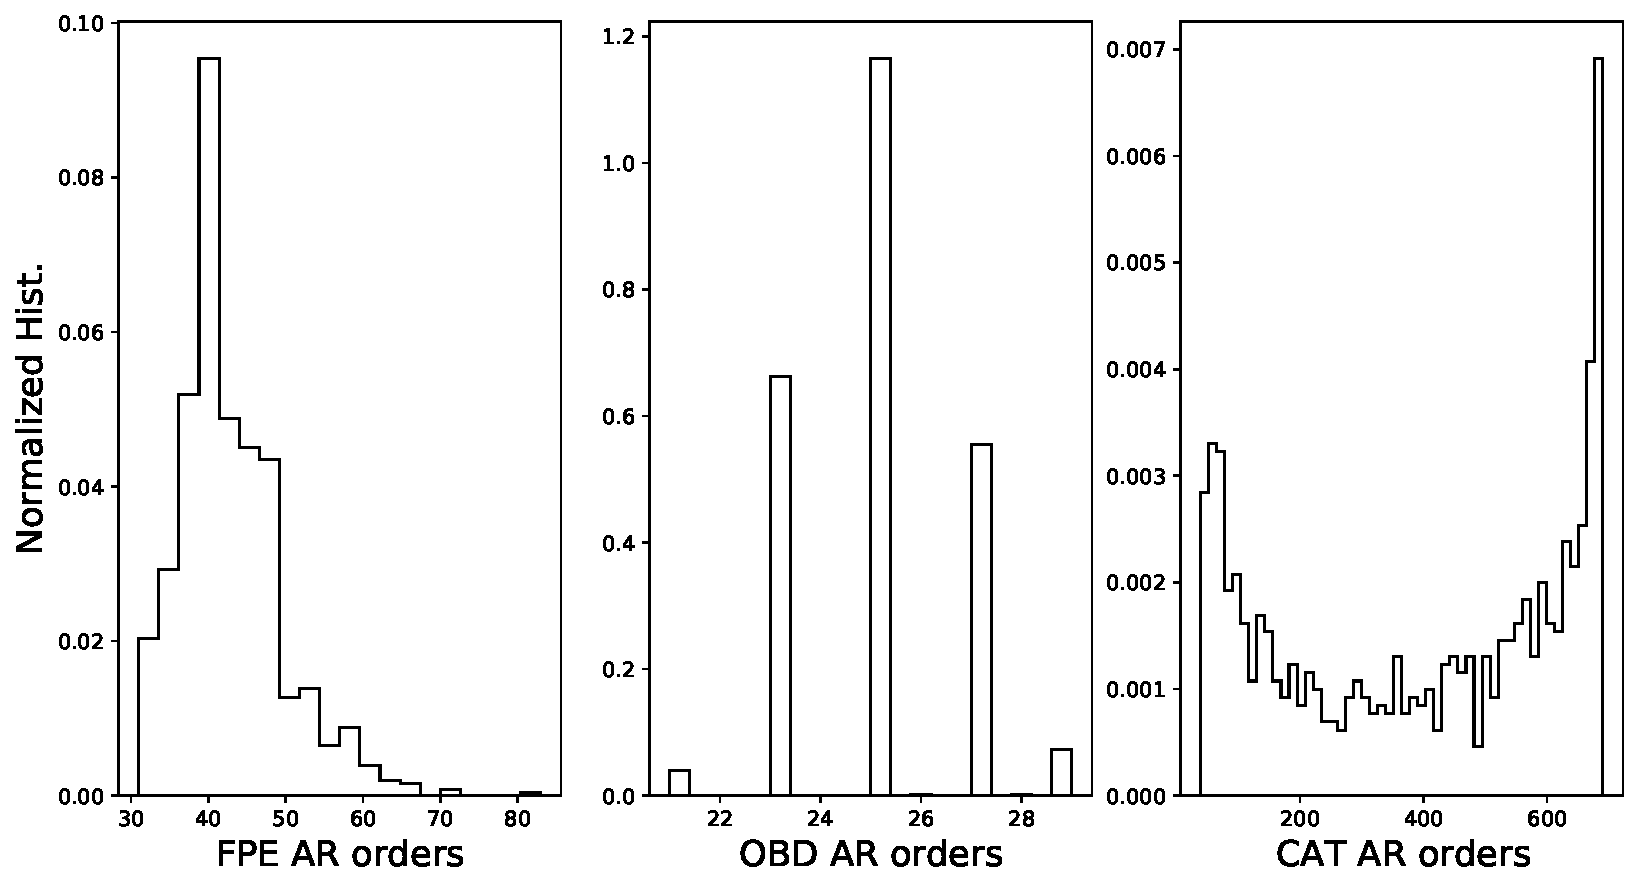
\includegraphics[scale = .45]{Images/NormalPSD/ordersComparison.pdf}
    \caption{Histogram of estimate orders for each method}
    \label{fig:ordersCompairson}

\end{figure}
definitely shows that FPE gives the best results: it is a stable method that choose filters in the clustered area associated with minimum error, while both OBD and CAT result lies outside this area and show bigger errors. Two other interesting plots that stress this fact are reported in figure \ref{fig:ordersCompairson} and \ref{fig:residualsComparison}
\begin{figure}
    \centering
    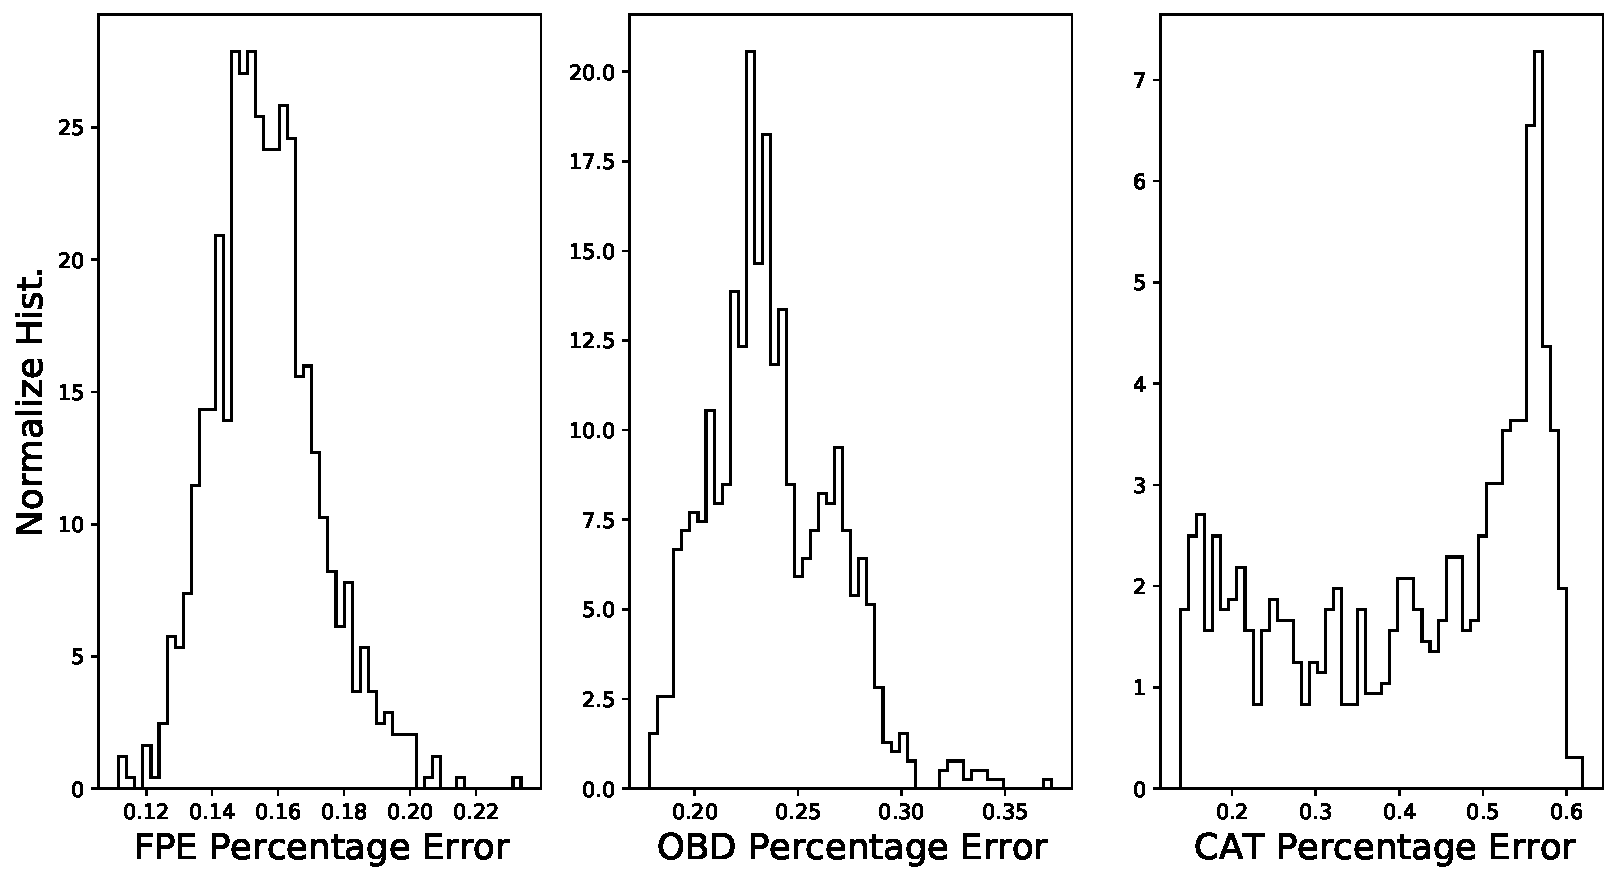
\includegraphics[scale = .46]{Images/NormalPSD/ResidualsComparison.pdf}
    \caption{Histogram of residuals for each method}
    \label{fig:residualsComparison}
\end{figure}
where the histograms for the errors and for order's estimate are reported. These graphs provide stronger evidence for our previous statements. As already noticed, FPE is very stable and provide the smallest 'overall relative error'. \\
CAT histogram shows a very interesting behaviour. The histogram for the order show two different peaks,  a small one associated to 'short filters', and a second high peak at $m = M$. This means that CAT is most likely to not converge at all at some value for the regression order, and it is more likely selects a length that is comparable with the largest available.  If short filters are selected, the overall percentage error will be low, respectively represented by the first peak in the distribution of the errors, while if long filters are selected, the error is maximized. 

So, even if in some cases CAT might be more accurate when taking the average over several spectra, FPE guarantees that minimum error will be reached. 

\subsection{Analysis of Ligo Spectrum}
\begin{figure}
    \centering
    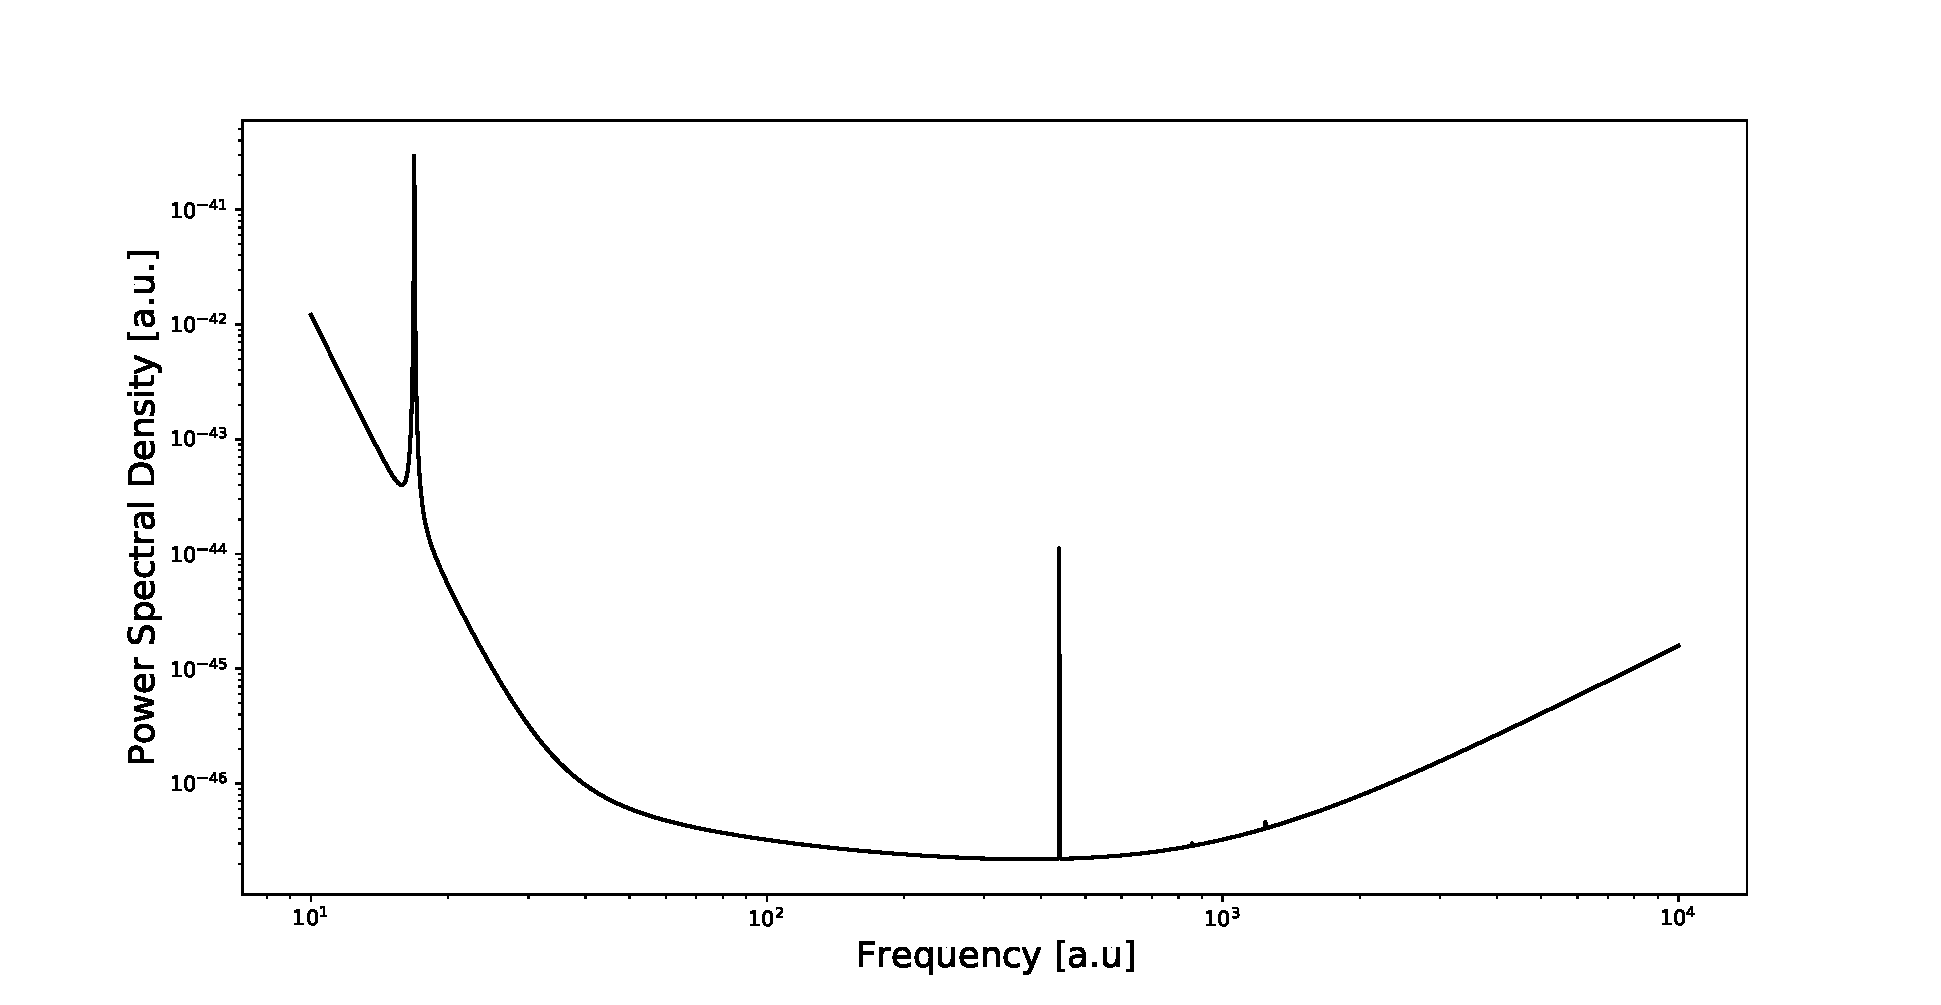
\includegraphics[scale = .45]{Images/LIGOsimulate/LigoPSDoriginal.pdf}
    \caption{Original power spectral density from Ligo}
    \label{fig:LigoPSDOriginal}
\end{figure}
In this subsection we concentrate again on the reconstruction of a specific, known, power spectrum.
We analyze the properties of reconstruction of this second spectrum whose shape is the Advanced LIGO design sensitivity theoretical spectral curve (Figure \ref{fig:LigoPSDOriginal}). 
For this analysis we will study properties only for arrays of 40960 points. We consider a sampling rate of $2048 samples / second$ that means we can reconstruct a Nyquist frequency of $1024 Hz$. We chose a longer dataset than before because algorithm works with a 1 dimensional interpolation of spectrum, and with shorter datasets the interpolated spectrum is not consistent with the original spectrum and does not capture the height of the peaks. Shorter choices would result in noise extracted from a different power spectrum than the one in figure \ref{fig:LigoPSDOriginal}. \\ 
We will study statistical properties from samples obtained with 500 simulations and compare the obtained results for each optimizer. 
We start considering statistical properties of mean spectrum obtained averaging over all the simulations and conclude with an analysis for the statistics of the reproduction of single spectrum. 
\subsubsection{Properties for the average spectrum}
Here we report mean properties of the reproductions of the spectrum. The spectrum we want to reconstruct is reported in Figure \ref{fig:ligospectrum},
\begin{figure}
    \centering
  
        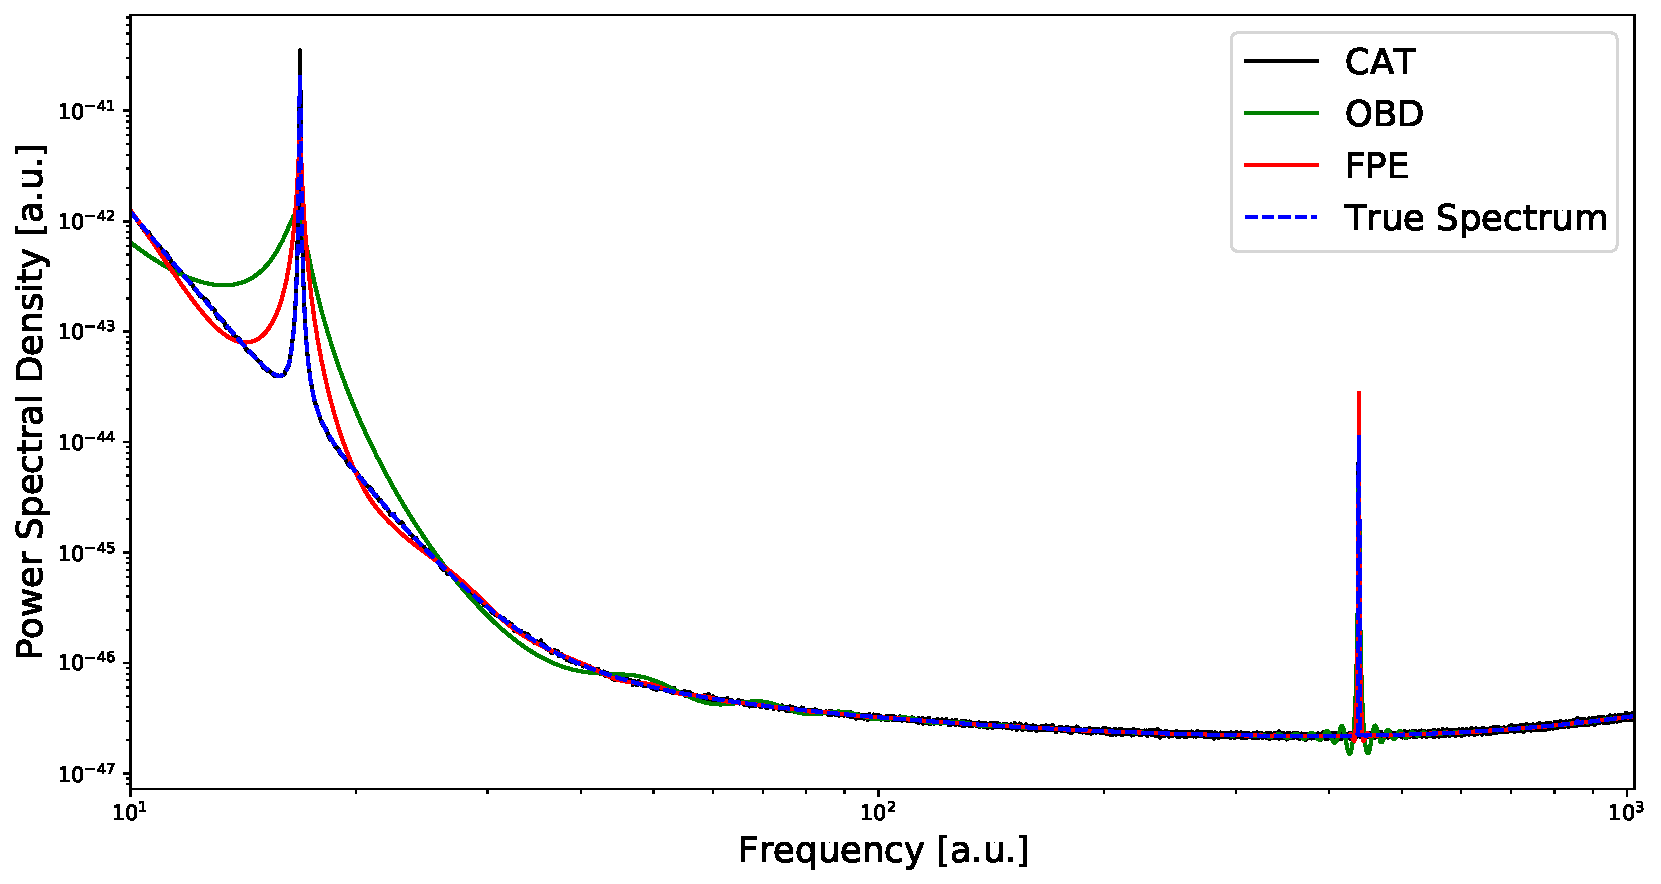
\includegraphics[scale = 0.45]{Images/LIGOsimulate/PSD.pdf}
        \caption{A priori spectrum from Ligo database}
        \label{fig:ligospectrum}
\end{figure}
shows the original power spectral density and the ensemble average of every method. For the mean, the relative errors are: 
\begin{equation}
    \bar r_{\bar S, FPE} = 0.0426\%, \qquad \bar r_{\bar S, OBD} = 0.129\%, \qquad \bar r_{\bar S, CAT} = 0.0211\%
\end{equation}
Again, if one only check overall accuracy for every method, CAT is outperforming. In fact, even in presence of very sharp peaks, CAT reconstruction seems to be almost perfectly coincident with each of them. To check this behaviour we take a look at the two peaks separately. For the first one a log plot of the reconstructed peaks and their relative errors are shown in Figure \ref{fig:ligo1peak} 
\begin{figure}[h]
        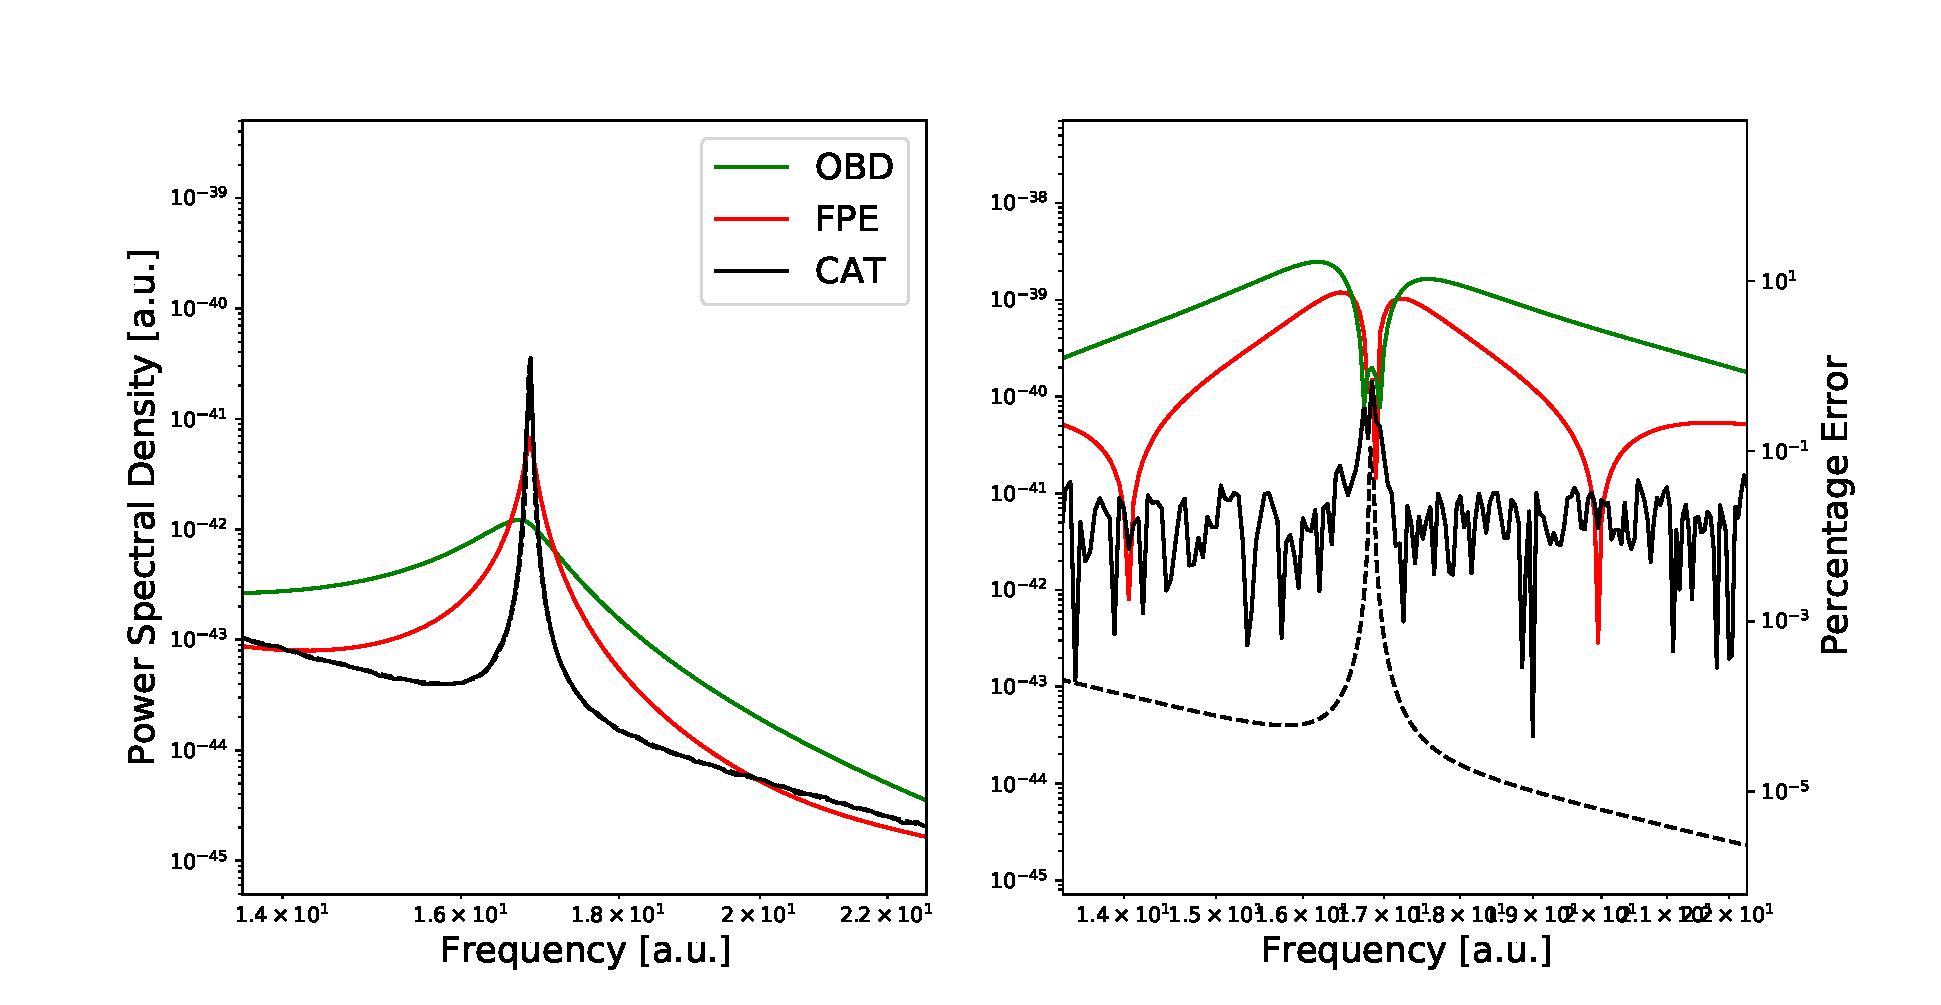
\includegraphics[scale = 0.45]{Images/LIGOsimulate/1stPeakComparison.pdf}
        \caption{1st peak of the spectrum and it reconstruction with every optimizer (left) and associated percentage error (right)}
        \label{fig:ligo1peak}
\end{figure}
and the results reinforce our previous statement. The behaviour of the error is very similar for CAT and FPE, showing similar shapes but very different sizes, while CAT is giving a different and way more precise result. Both FPE and OBD are not able to capture the width of the peak and also show larger errors, while CAT has a good behaviour in reconstructing width's also. 
The reconstruction for very sharp peaks considering the average over all the spectra is found to be strongly inaccurate for both FPE and OBD, while a good accuracy is reached with CAT method. \\ 
Considering the estimate for the position of the peak, whose true value is found to be $16.85 \quad a.u. $, within numerical accuracy both FPE and CAT find its exact position, while OBD shift the peak left at $16.7 a.u.$, with a $0.9\%$ inaccuracy.\\ 
Second peak results are analogous, plotting the peak and the errors value around it
\begin{figure}[h]
    \centering
        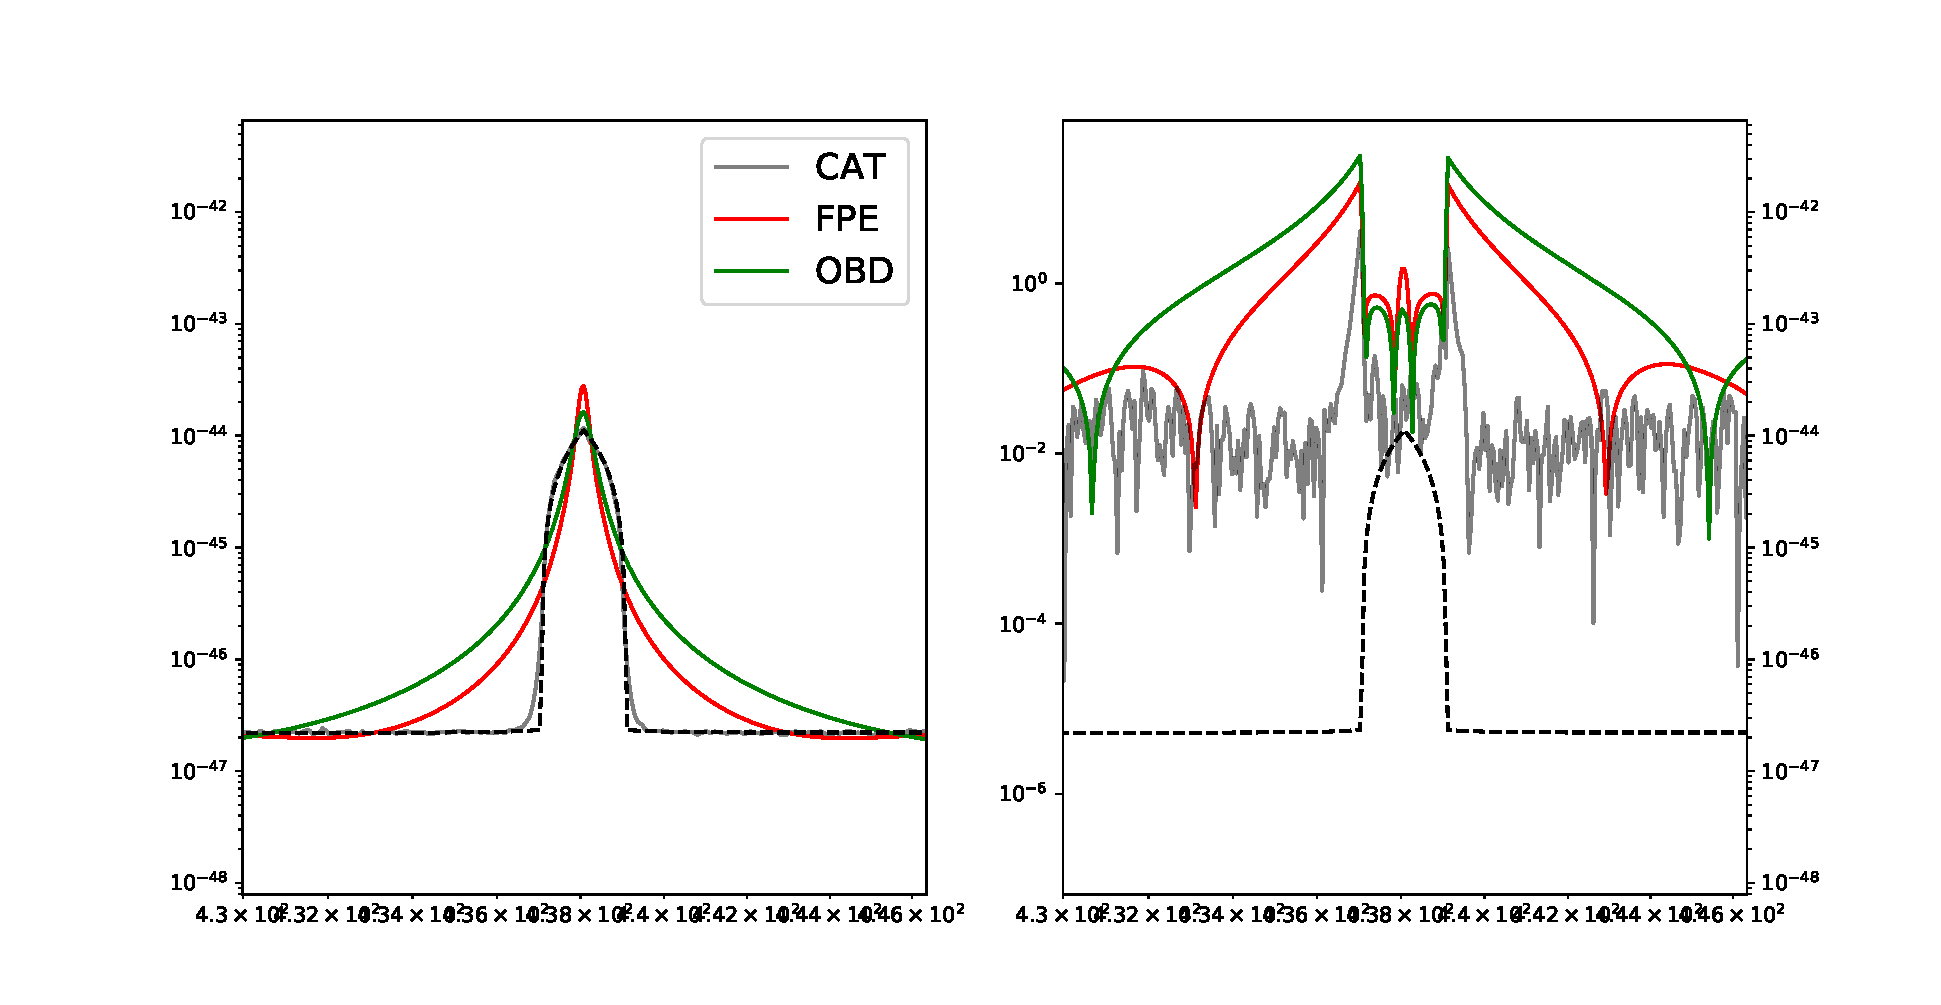
\includegraphics[scale = 0.45]{Images/LIGOsimulate/2ndPeakComparison.pdf}
        \caption{2nd peak of the spectrum, Relative error around 2nd peak of the spectrum}
        \label{fig:ligo2peak}
\end{figure}
we find again that FPE and OBD are performing similarly, the magnitude of the error is maximum for OBD and minimum for CAT. \\ 
In this case even CAT shows large errors in some points, but they are reasonable in a large part of it, still, it remains the best reconstruction.  For this second peak, all the methods find maximum position to be at $438.05 \quad a.u.$, which is the true position of the maximum.
Looking at Figure \ref{fig:ligo1peak} at \ref{fig:ligo2peak}, it appears to be clear that the least of the accuracy is not on the peak, but immediately around, so that one of the biggest deal is the reconstruction of peak's width, that only CAT is able to capture with high definition. \\ 
Even if FPE shows larger error in the peaks than CAT, when the average over all the frequencies is considered, their percentage errors are of the same order of magnitude. This means that outside the peaks FPE is more accurate than CAT, i.e. CAT is still giving noisy results.\\ 
As for the normal distributed noise, mean spectrum is not sufficient to declare what is the best optimizer to be used, since most of experiment are purely observational and mean spectrum over different realizations of the same stochastic process cannot be computed. So, it is important to also understand what is their behaviour for single realizations of the process.
\subsubsection{Statistical properties of single realizations} 
The errors for the single realizations behave very differently from the errors obtained when we considered the mean spectrum. In computing the mean of the overall errors for each single spectrum, the results we obtain are the following:
\begin{equation}
    \bar{r}_{FPE} = 0.13 \pm 0.01; \qquad \bar{r}_{OBD} = 0.17 \pm .02; \qquad 
    \bar{r}_{CAT} = 0.4 \pm 0.1
\end{equation}
where the error is just the standard deviation of the samples.
In this case we find a different result: FPE shows the best results and order's estimate is associated with least errors. Also, having found a smaller standard deviation of the datas, we can state that FPE and OBD are more stable optimizers then CAT. In fact, their properties as a function of filter's length are almost identical to those obtained in the study of normal spectrum. If we again plot the value of the errors as a function of the estimate of the order (Figure \ref{fig:LigoOrderError})
\begin{figure}
    \centering
    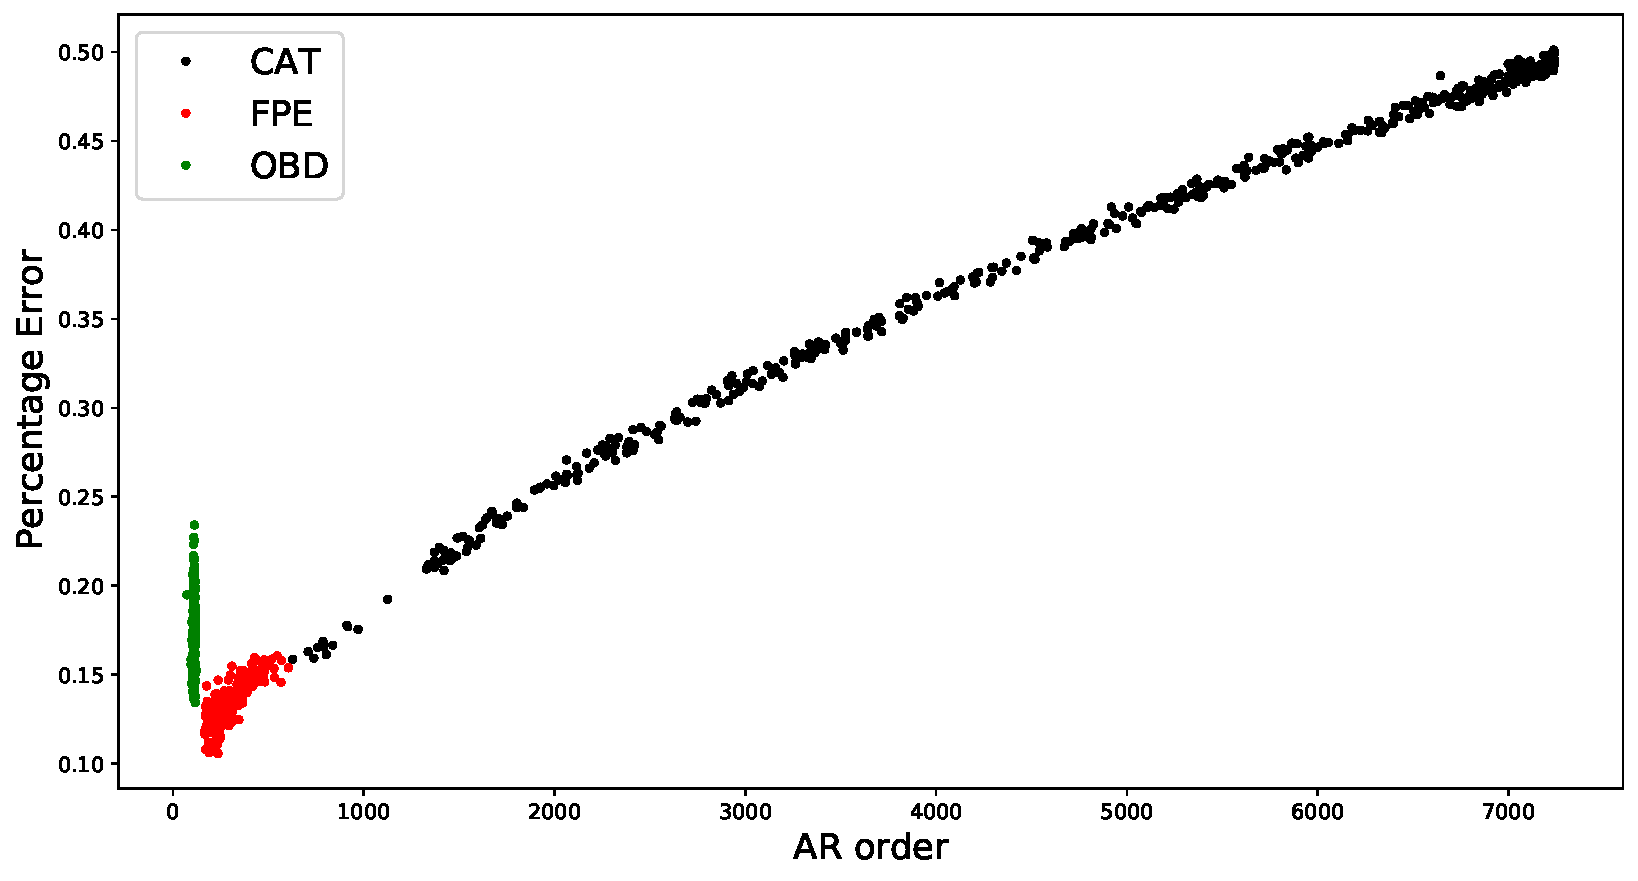
\includegraphics[scale = .43]{Images/LIGOsimulate/orderVSerror.pdf}
    \caption{Plot of relative error as a function of the estimate for filter's length}
    \label{fig:LigoOrderError}
\end{figure}
it is immediate to see that, again, FPE results lies in the are of filter's length associated with a minimum of relative errors, OBD lies in a clustered window with a higher error and CAT is not convergent, but most of the results are outside the minimum error area. So, we arrive at the same conclusion we had when we considered the normal specturm. OBD has no general properties that make it a preferable optimizer then FPE or CAT while, what to choose beneath the last two is based on the problem we are dealing with: if we have one single realization for the process, we are mostly sure that FPE would catch the area associated with the best resolution possible, while CAT would result in a spurious result with, in general, a not so good resolution. But, in case we have several realization for the same process, this last property of CAT, together with its instability, result to be his luck and, taking the average errors tend to compensate noise in the result, originating a very well defined spectrum that show same resolution almost everywhere, no matter how small the values are (as for normal PSD case) or how sharp peaks can be, the result has got generally good accuracy, also if it is clear that we have to pay this fact with very large error bars. So a choice between these methods is a matter of convenience and interest for each specific problem. \\
\begin{figure}
    \centering
    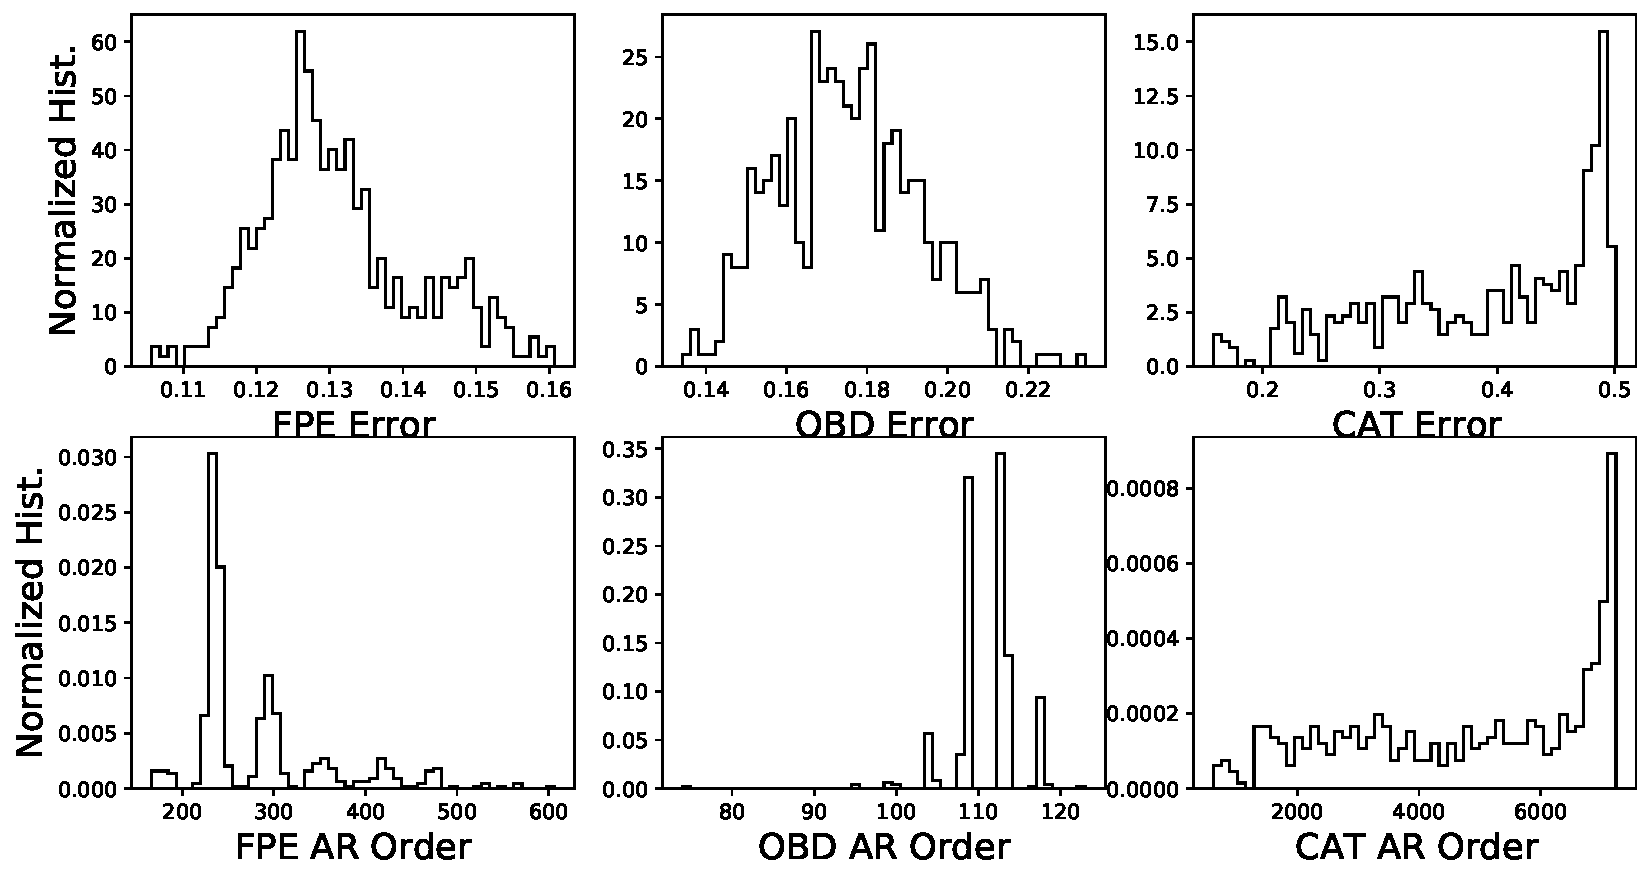
\includegraphics[scale = .43]{Images/LIGOsimulate/LigoHists.pdf}
    \caption{Histograms showing the estimate for the autoregressive order and overall percentage error obtained with all the three optimizers.}
    \label{fig:my_label}
\end{figure}

\section{Another approach to CAT} \label{sec:ACAT}
We stated that, if one consider a single realization for some stochastic process the choice for the optimizer should rely on FPE because of its stability and better single estimate, while CAT, when applied on a single dataset, does not assure a good resolution for our estimate. \\
It was found that CAT shows its best properties when considering the average over a big number of reconstructions, where noisy results tend to compensate each other reaching a very good quality reconstruction even for not too long arrays (as in the case of Gaussian PSD where we considered simulations of 3000 points). This led us to propose another approach to CAT: instead of applying Burg's method on the whole data set, we can divide it in smaller arrays of data and apply it to each one of them taking their mean at the end of the computation. In this way, accuracy can be made incredibly higher than the one obtained with the standard approach. \\ 
Unluckly, it is very hard to investigate how one should divide the dataset to reach minimum error. If one consider a known power spectrum, the problem could be solved numerically, but unuckly in real life experiments we do not know what true spectrum is, and such an approach is non-sense. \\ 
The non linear form for the estimator together with the finite-order recursion make it hard or even impossible to find general properties for the estimate, and so we will not investigate many of that questions that could arise.\\
For examples, what is the best choice for the length of the sub data-set? If we choose too short arrays, we will mediate over a lot of different spectra, decreasing variance, but it is probable that we will not be able to capture all the features of the spectrum. Too long subsets, instead, would result in too few reconstructed spectra, so that taking their average would not reduce variance in a significant way. It seems a very hard task to answer this question uniquely, and maybe such an answer does not even exist in a general case. One prescription on the length of the sub arrays may concern some consideration about frequencies: if we want to accurately reconstruct low frequency behaviour, one has to make long time observations, so for those cases longer datasets are required.  
Since taking overlapping arrays does not seems to affect negatively single estimates, this could be a good prescription to maximize the number of reconstructions for a given length. \\
Stressing to its maximum the hypothesis that such a procedure is harmless, one could try any overlapping sequence to maximize the number of reconstructions. To study this approach, since we want every reconstruction to be more than slightly different from each other, we chose an overlapping that is half the length for the sub arrays. 
We test this new approach on LIGO dataset on the same noise simulations as before. We chose sub segments of length L = 3000, 5000, 7000 and 10000.. \\
In figure \ref{fig:alternativeCAT} we compare the result associated with with this new approach for the lengths written above. For each of the 500 reproductions, we chose the one associated with the median overall error. 
\begin{figure}
    \centering
    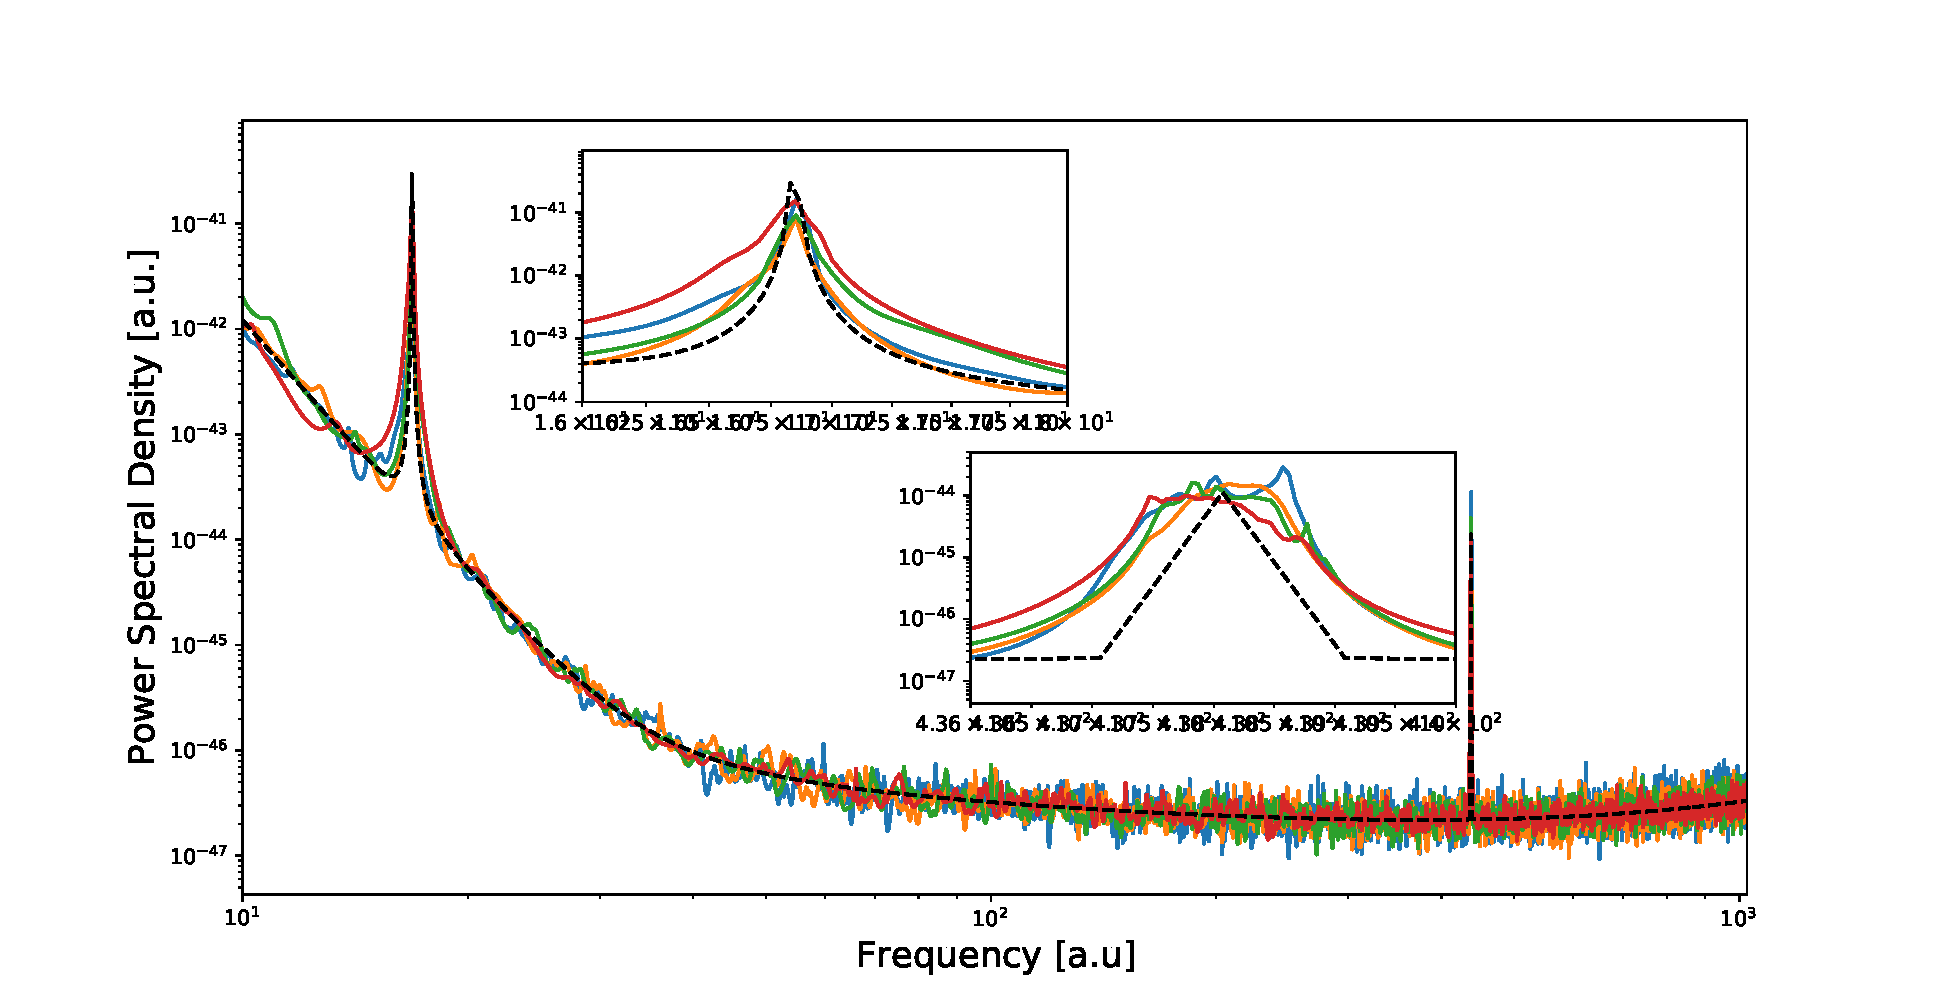
\includegraphics[scale = .45]{Images/AlternativeCAT/AlternativeCAT.pdf}
    \caption{Alternative CAT approach to Ligo Spectrum for different lengths of the sub arrays}
    \label{fig:alternativeCAT}
\end{figure}
As one can expect from CAT behaviour results obtained with larger arrays are associated with increasing noise. Considering the reconstruction for single peaks, it is found that accuracy is certainly dependent from the length, but it seems to give the best result for $L = 7000$, and not for $L = 10000$ as we were expecting. This difference can be understood if one considers the number of realizations over which we take our average: for arrays of $7000$ points we are taking the average over 12 different realizations, while for arrays of $10000$ points we are taking our average on eight different realizations only. This is probably the reason why this higher length is not associated with higher resolution. 
We clearly see that the reconstruction achieved using $L = 7000$ is the best in capturing the width of the peaks and their position, but none of the reconstructions is able to accurately reproduce the second peak. 
We want to compare these results with the standard approach, and with both the results obtained with FPE and with CAT. 

\subsection{Alternative CAT vs FPE}
The first comparison we make between FPE and alternative CAT regards the distribution of the overall errors. 
\begin{figure}
    \centering
    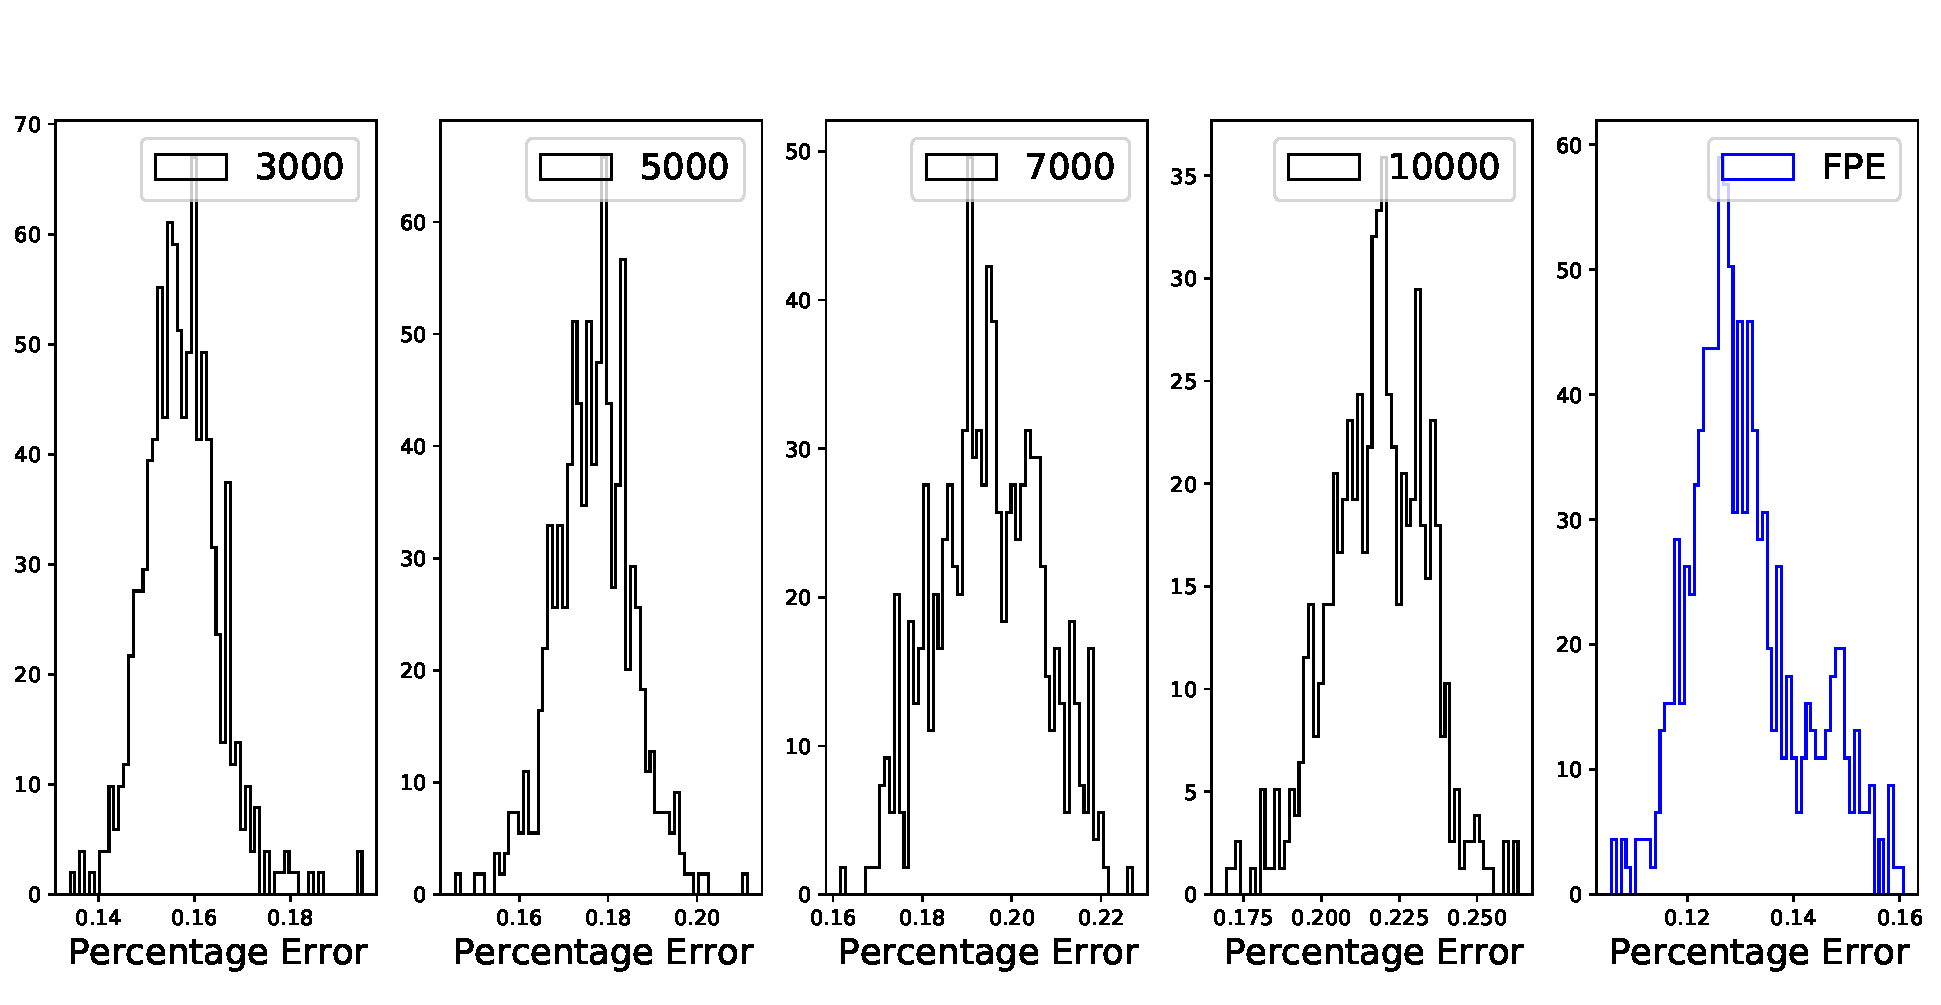
\includegraphics[scale = .45]{Images/AlternativeCAT/histACatVSFpe.pdf}
    \caption{Histogram of the percentage error as a function of the length of the sub arrays. The blue panel shows the histogram obtained from FPE}
    \label{fig:aCATvsFPEhist}
\end{figure}
Figure \ref{fig:aCATvsFPEhist} shows the distribution of the percentage error as a function of the length of the segments of the data. The support of the histogram is, for every length, shorter than the support the one expect to be obtained with CAT (y-axis of figure \ref{fig:LigoOrderError}), so that this approach is found to be more stable than standard CAT. \\ 
Shorter arrays are found to minimize the error, as could be expected from the fact that the variance is reduced from this choice, but non of the chosen lengths reaches the overall accuracy of FPE. \\ 
From the previous histograms, the most meaningful comparison of FPE with alternative CAT is obtained using as preferable length the reconstruction '3000'. \\ 
The mean and standard deviations of the percentage error are, in the two cases 
\begin{align} 
    \bar &r_{FPE} = 0.13; \qquad 
    \sigma_{FPE} = 0.01 \\ 
    \bar &r_{aCAT} = 0.158; \quad 
    \sigma_{aCAT} = 0.007
\end{align}
With this alternative approach, we have been able to obtain reconstructions for the spectra whose accuracy is almost comparable with the one obtained with FPE. But the comparison of the overall error is just a rough indicator of the accuracy in the reconstruction, for that reason we compare the median error reconstruction of both methods. 
\begin{figure}
    \centering
    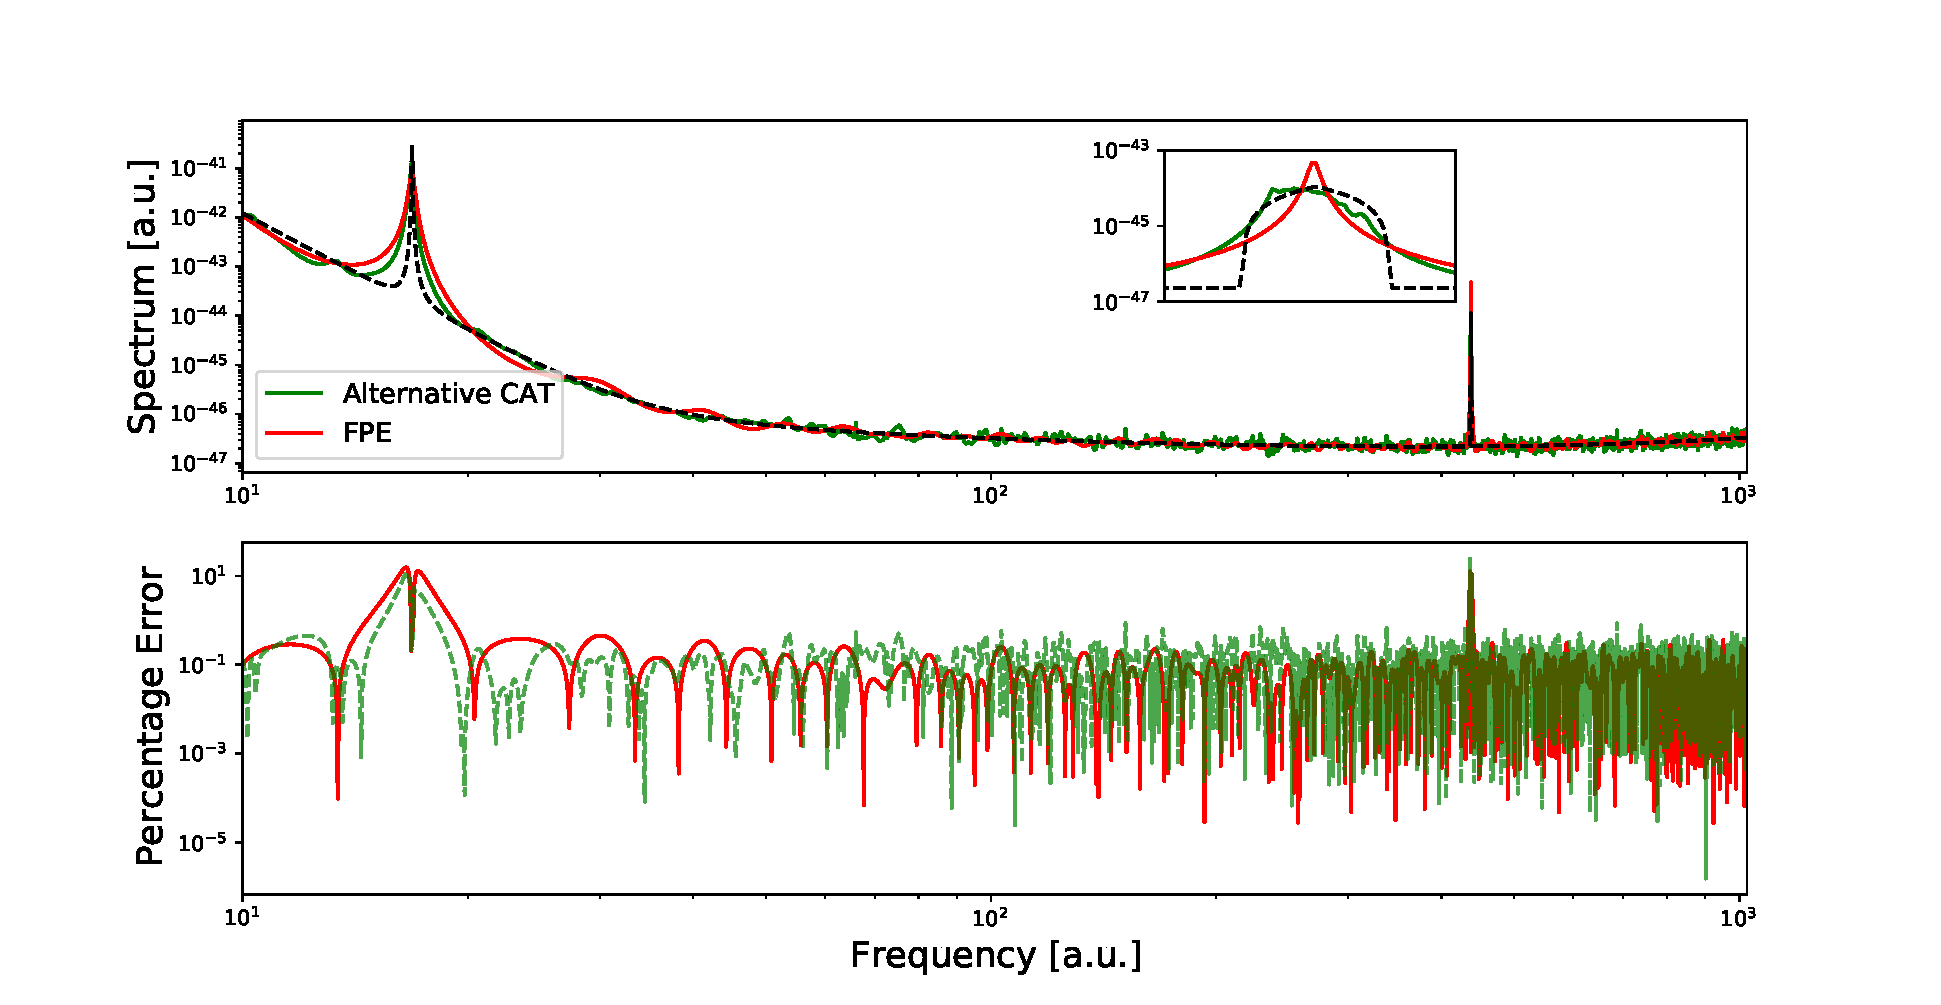
\includegraphics[scale = .45]{Images/AlternativeCAT/FPEaCATwhole.pdf}
    \caption{Comparison of FPE method with alternative cat with length of 3000 points (above panel) and their percentage error (below panel)}
    \label{fig:aCATvsFPEwhole}
\end{figure}
Figure \ref{fig:aCATvsFPEwhole} shows both the reconstruction obtained with FPE and alternative CAT (above panel) and the percentage error for each frequency (below panel). It is evident that the two result are very similar. Alternative CAT provides a sightly better accuracy in the reproduction for the first peak. But, for the rest of the reconstruction FPE has to be preferred. Regarding the second peak, FPE accuracy is largely better. Alternative CAT flattens the peak and its maximum is not localized, while the reconstruction of FPE is representative of true position of the peak. Also, in the rest of the spectrum the result of FPE still shows less noise. \\ 
From thie brief comparison, we can conclude that alternative CAT approach shouldn't be used with "short" arrays (short with respect to the total length N of the time series), since FPE provides a better estimate. \\ 
Since for short arrays the best quality is still achieved by the use of FPE, a second interesting comparison is the one between FPE with the alternative CAT estimate on longer arrays. From figure \ref{fig:alternativeCAT}, it is evident that the best compromise between noise and accuracy in the reproduction is obtained by the arrays of 7000 points. It is clear that, outside peaks, the smaller error is achieved by FPE, so that te interesting part will be the expected gain in the definition of the peaks.
\begin{figure}
    \centering
    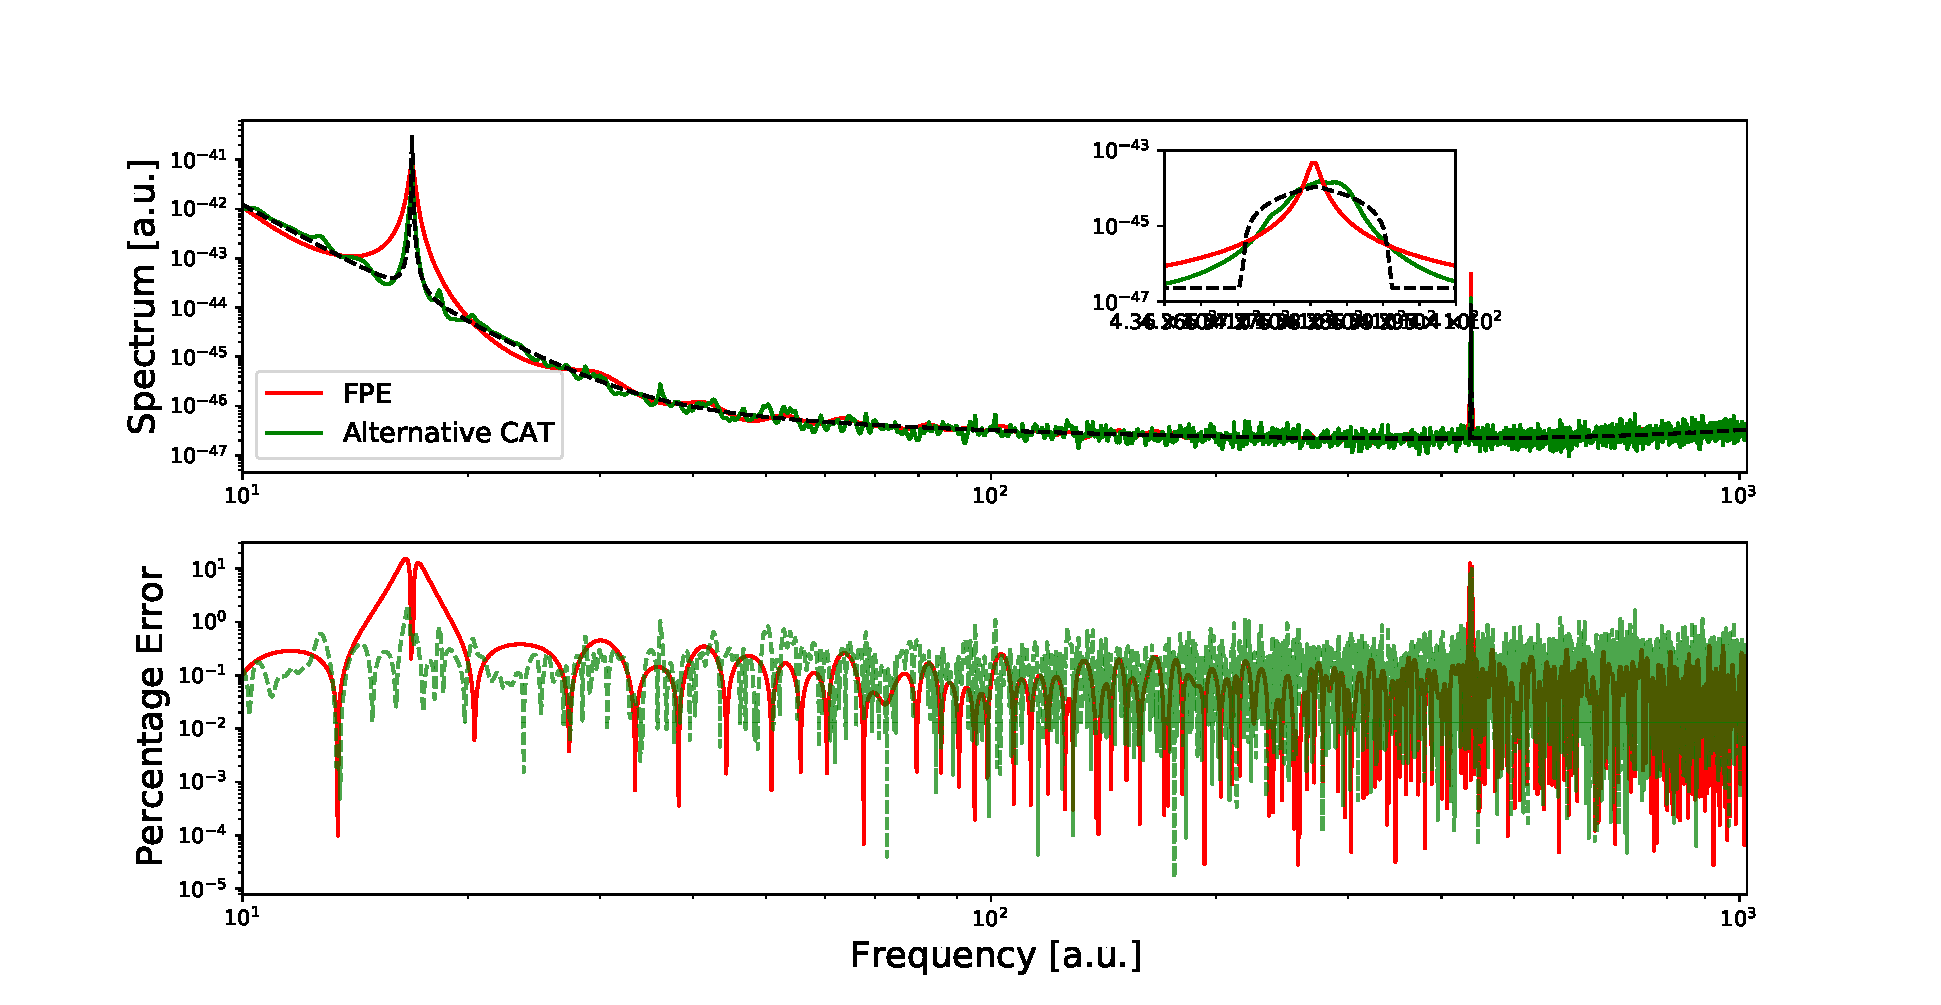
\includegraphics[scale = .43]{Images/AlternativeCAT/FPEaCAT7000.pdf}
    \caption{Comparison of the alternative CAT with 7000 points subsegments of data with FPE}
    \label{fig:aCAT7000FPE}
\end{figure}
Figure \ref{fig:aCAT7000FPE} shows the reconstruction obtained with FPE (red line) and the one obtained with the alternative CAT approach, for sub-segments of 7000 data and a 50\% overlapping. This result is more interesting than the previous. As expected, the noise in the reproduction is larger, as can also be noticed looking at the error in the below panel, but the introduced noise is a reasonable quantity.  Concerning the peaks, the first peaks reconstruction has gained a large accuracy in the reproduction, for both its width and position. The second peak is reconstructed in a comparable way for both the methods. FPE captures in a better way the position of the peak, while alternative CAT gains in the reproduction of the width and general shape. \\ 
Concluding, this new approach might be a valid alternative to FPE if 'not-too-short' sub segments of data are chosen. In this way, introducing a reasonable amount of noise, we are able to capture some details with more accuracy.
But if we deal with shorter datasets, like 3000 points, without any a priori knowledge on the shape of the spectrum, is this alternative method convenient? In chapter 4 we will see that this method is the best to characterize brown noise spectrum even with dataset of $1000$ points only, but such an investigation would require a long analysis and would deviate too much from our main interests. 
Since FPE has minimum requirement of external input we will prefer this standard approach, even if this alternative approach seems to have its merits. 
\subsection{Alternative VS Standard CAT}
We now compare the performance of this alternative approach with the standard approach with CAT optimizer. 
\begin{figure}
    \centering
    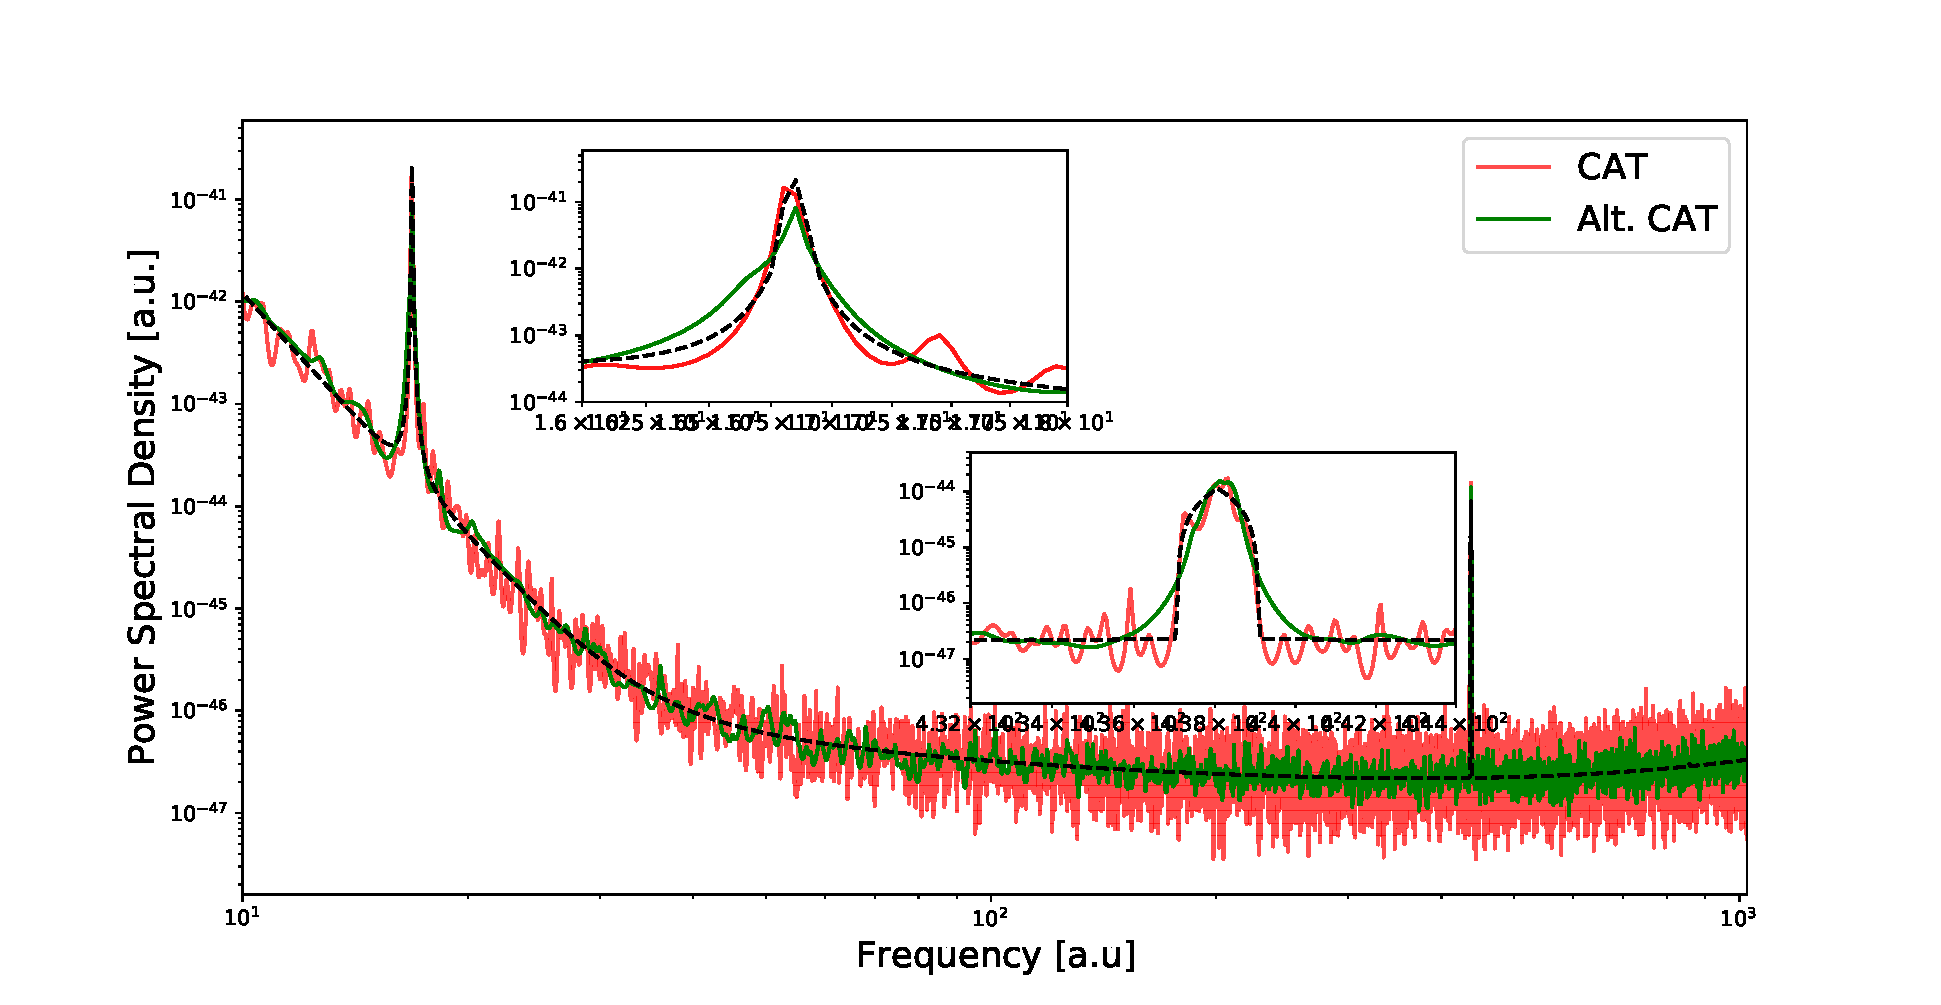
\includegraphics[scale = .45]{Images/AlternativeCAT/AlternativeVSstandard.pdf}
    \caption{Spectral reconstruction obtained with standard CAT approach and alternative approach}
    \label{fig:alternativevsstandard}
\end{figure}
Figure \ref{fig:alternativevsstandard} show that the alternative approach provides a reconstruction that presents a largely decreased quantity of noise. This decreased level of noise has as counterpart a decreased accuracy in the reconstruction of the width of both the peaks. But, even with this loss, the estimate is still very representative of the obtained spectrum, and might be a good price to pay to reduce the variance of the estimate.
\begin{figure}
    \centering
    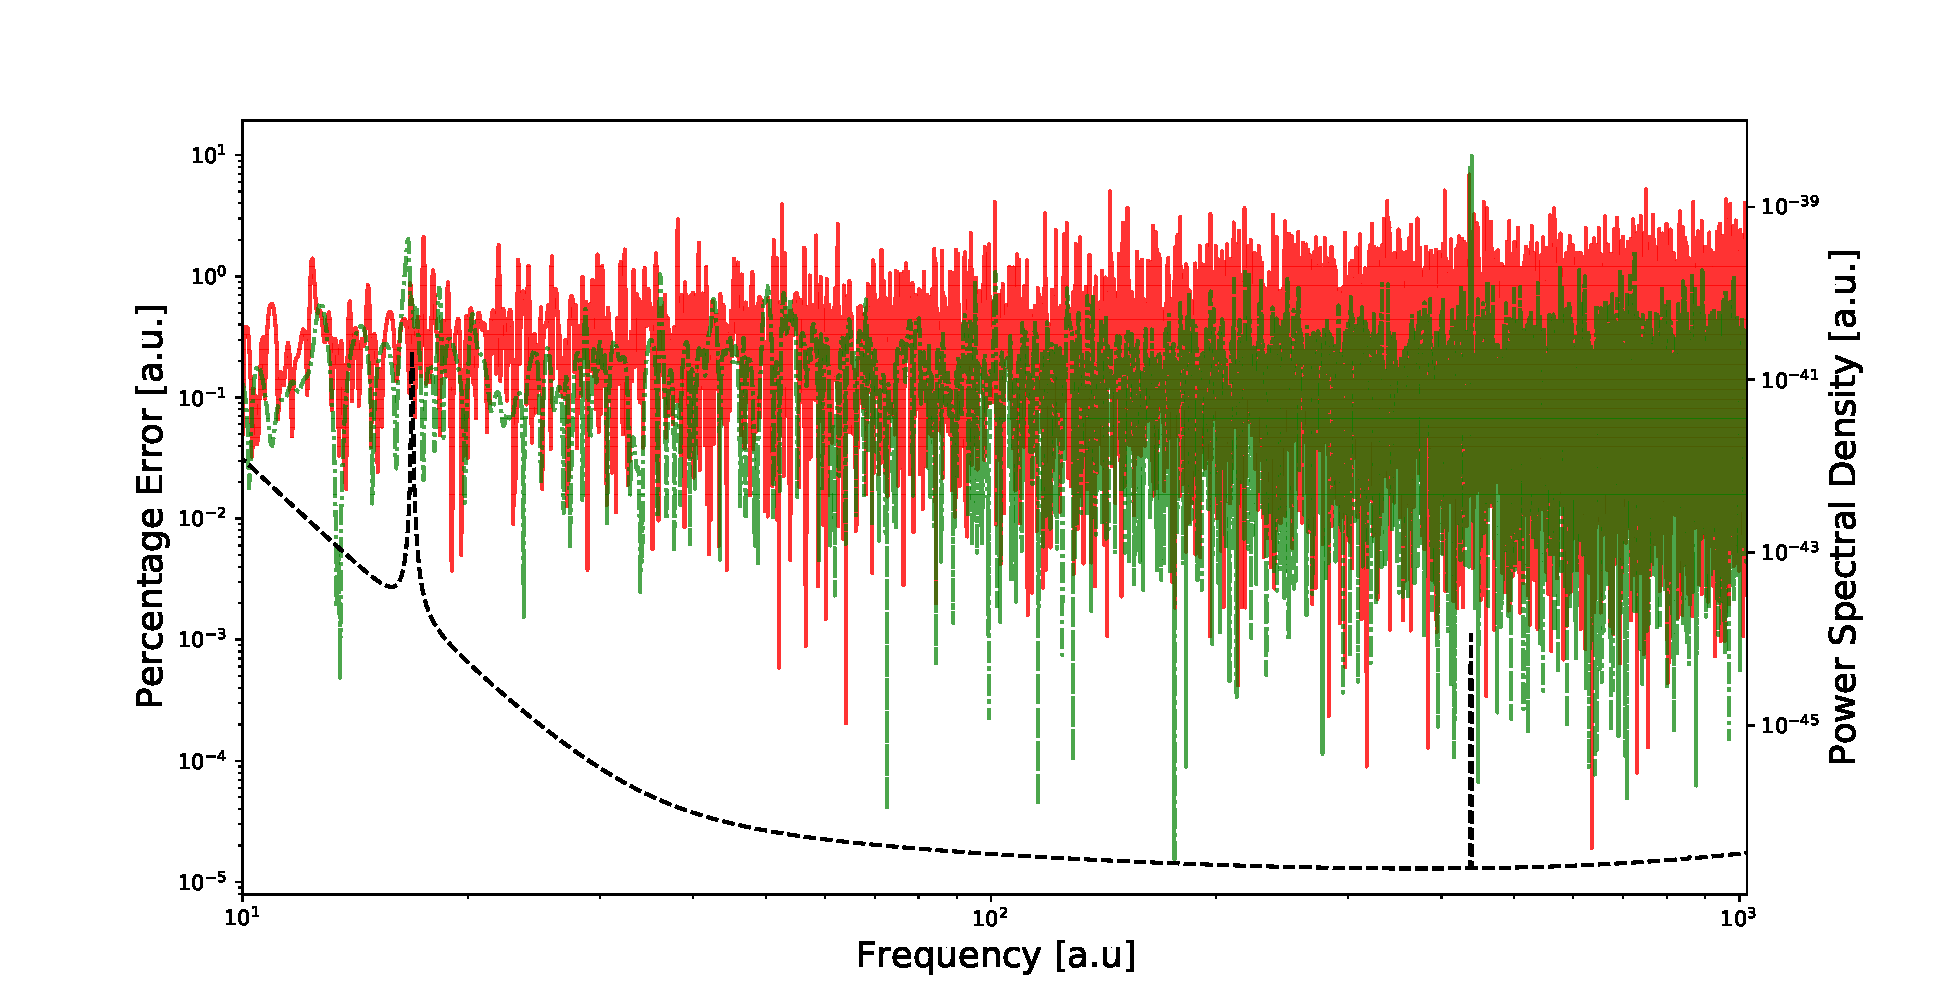
\includegraphics[scale = .45]{Images/AlternativeCAT/CATvsALTerrors.pdf}
    \caption{Percentage error of spectral estimate with CAT (red) and alternative CAT (green) }
    \label{fig:CATALTerrors}
\end{figure}
Figure \ref{fig:CATALTerrors} shows that loss in the definition due to the averaging over the subset is concentrated in a very small number of points of the estimate, and  negligible with respect to the gain obtained in the whole spectrum. \\ 
In this case, the reduction of noise is important because we selected the spectrum associated with the median overall error, highly influenced from noise. If CAT is 'lucky enough' to select filters whose length is comparable with FPE, probably such an achievement wouldn't be reached, but we expect the alternative estimate won't show any big loss. So, since this alternative approach gives better result for long filters and comparable results for shorter filter, being also more stable, is probably to be preferred to the standard approach with CAT as optimizer.
Clearly, such an approach has a great disadvantage: we lose all the information regarding the prediction error filter. So, if we want to characterize the process, FPE is with no doubt the best choice. While, if we are only interested in reconstructing the power spectral density, alternative CAT's approach might be worth an attempt. 
\section{Comparison of MESA with Welch Method}
We now compare the performance of MESA algorithm with estimate obtained with Welch method \cite{Welch1967}. Welch introduced his method in 1967, and it is based of Fast Fourier Transform. 
Estimate is obtained averaging over modified peridiograms computed on subset of the original dataset. Here, as in the alternative approach to CAT, one has to choose an opportune length for the arrays and their overlapping. Else, a window is required to emulate period of the Fourier Transform, and with this choice one is obliged to assume data to be zero outside this window. The shape of the reconstruction is strongly dependent from window's choice, so, in general, Welch method is not a stable estimate of the spectra, since it strongly depends on this arbitrary choice. We compare the reconstruction obtained with the two methods in figure \ref{fig:WelchVSfpe} 

\begin{figure}[H]
    \centering
    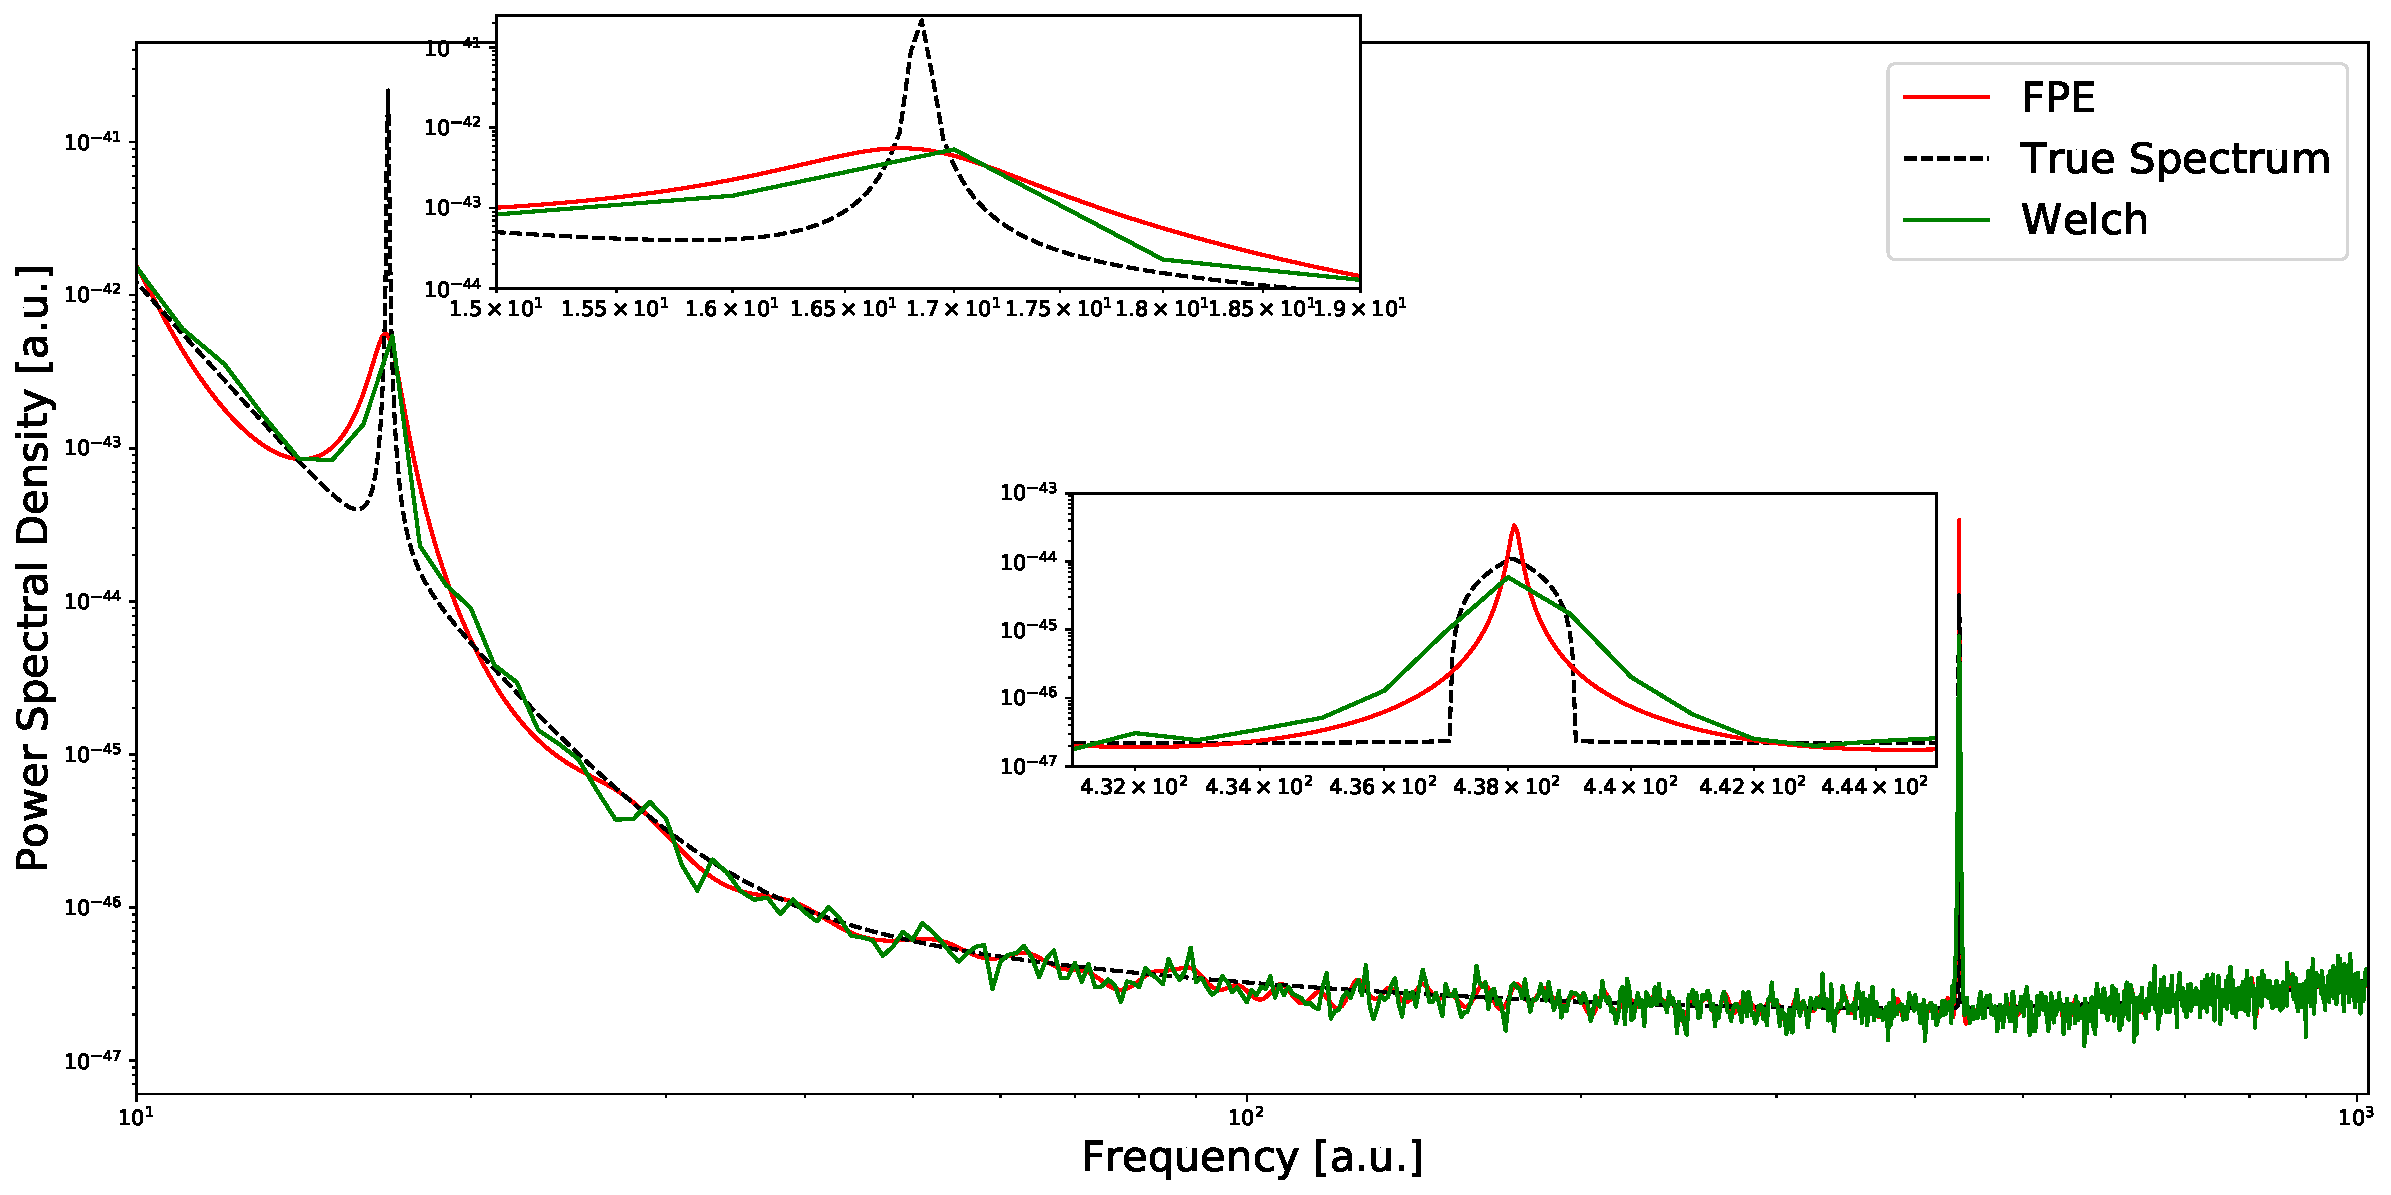
\includegraphics[scale = .3]{Images/WelchVSfpe.pdf}
    \caption{Comparison of the reconstructed spectrum obtained with FPE (red line) and Welch's method (green line)}
    \label{fig:WelchVSfpe}
\end{figure}

Graphically both methods are found to perform similarly. Since MESA is analytical, graph obtained with this method is smoother than one obtained with Welch. In fact, Welch spectrum is obtained performing a FFT and so its output length is related to the length of the subsets. Computing percentage errors, we obtain
\begin{equation}
    \nonumber
    \bar r_{MESA} = 0.11; \qquad \bar r_{Welch} = 0.26
\end{equation}
so that better overall accuracy is reached with MESA. A plot of both the errors of FPE and Welch method is reported in figure \ref{fig:WelchError}

\begin{figure}
    \centering
    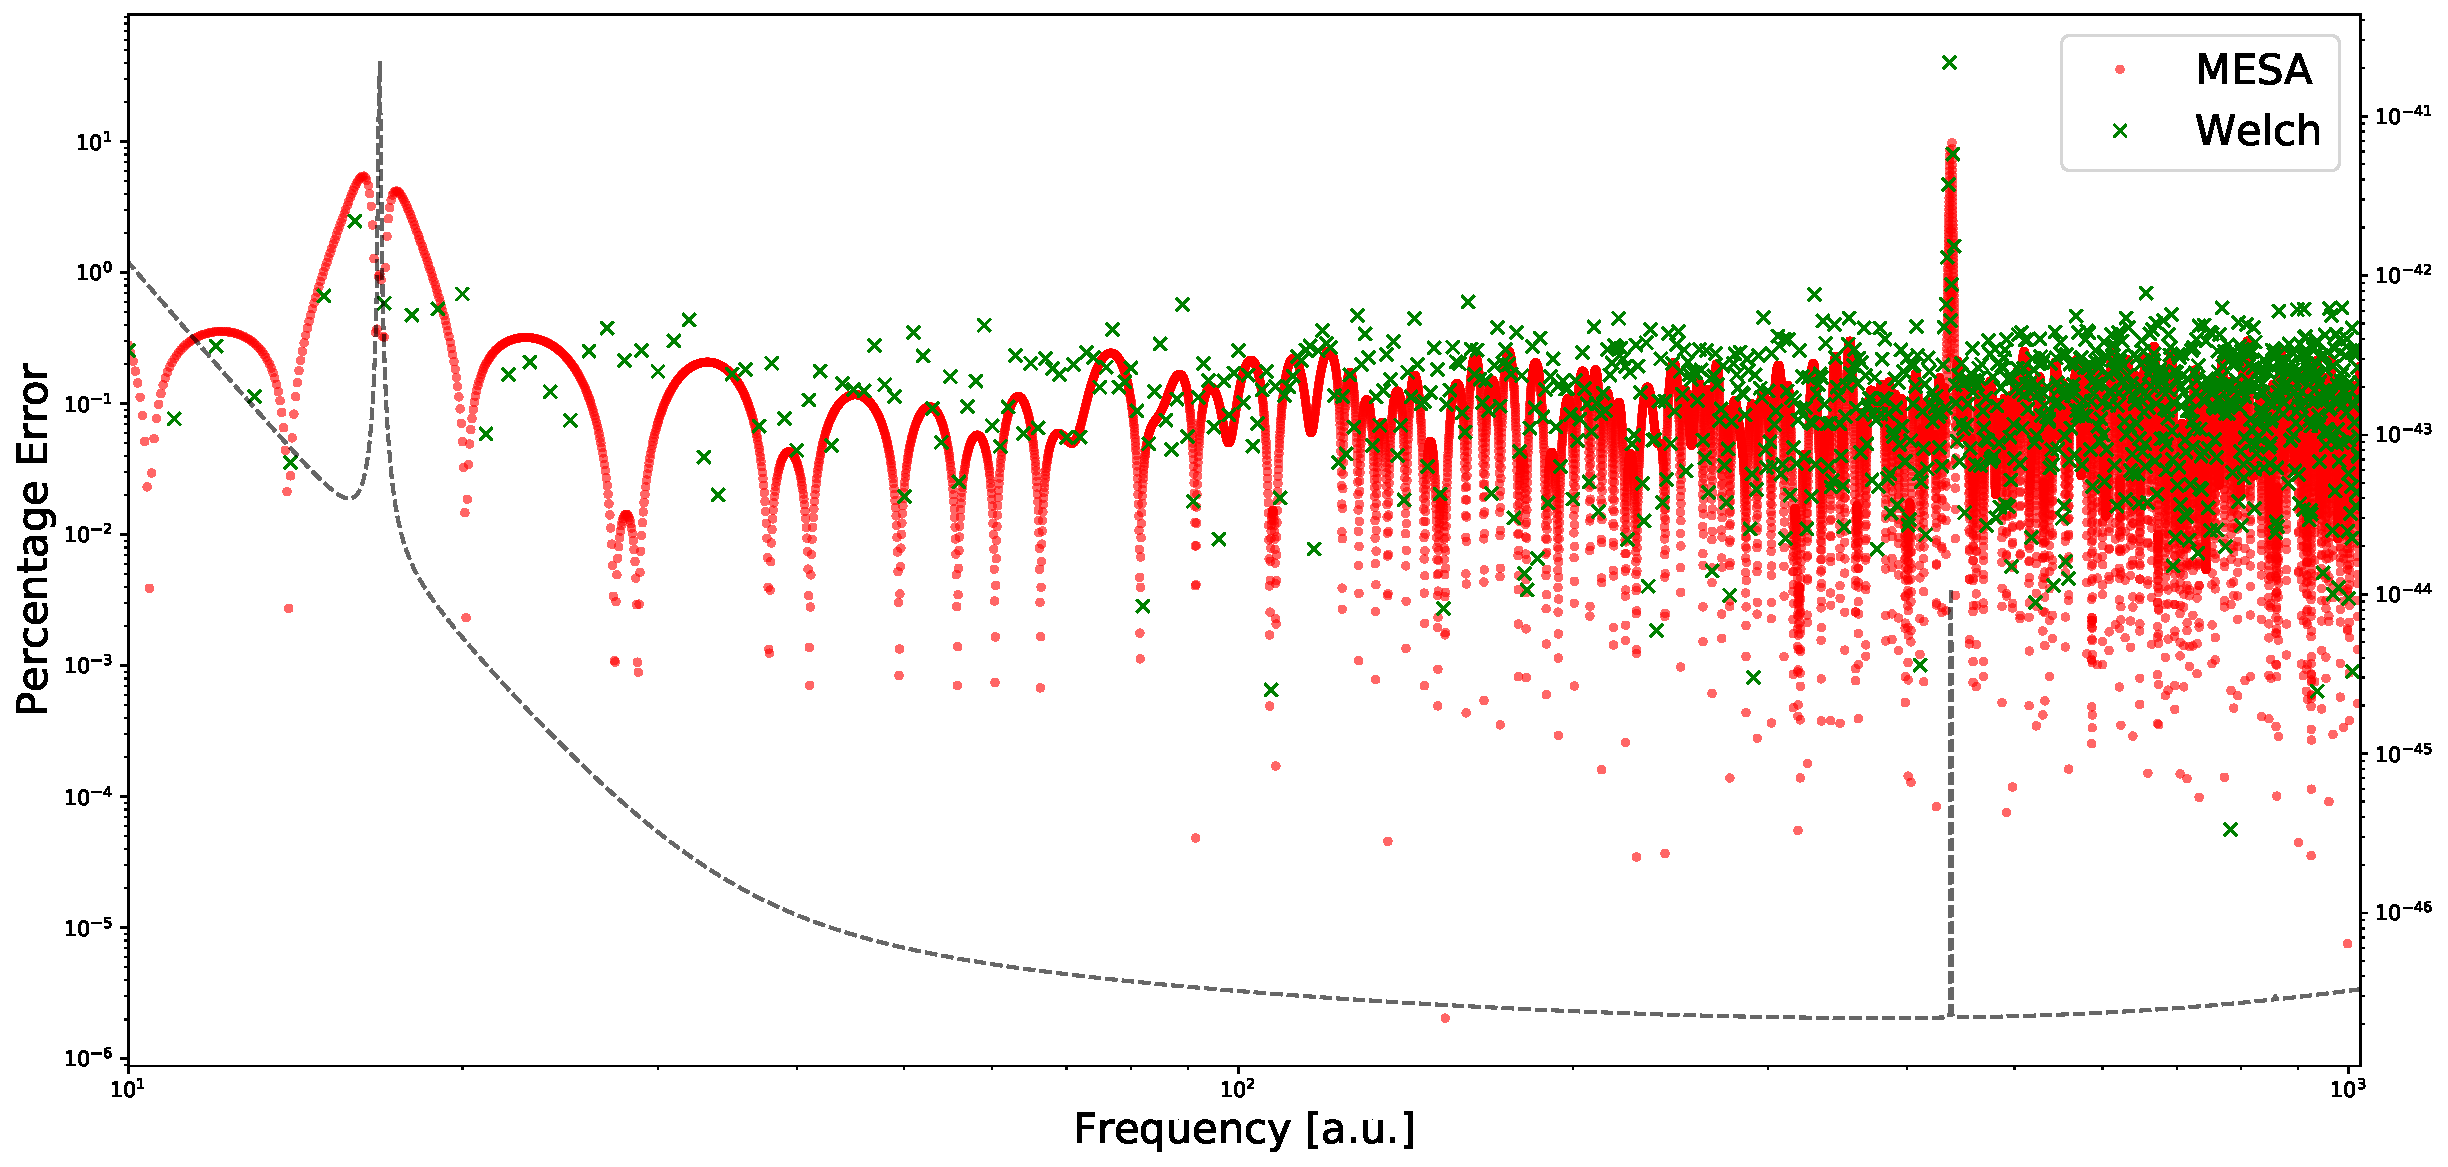
\includegraphics[scale = .3]{Images/WelchErrors.pdf}
    \caption{Comparison of percentage error of reconstruction with MESA and Welch method}
    \label{fig:WelchError}
\end{figure}It is evident that greater error for Welch is due to two main reasons. First reason is the reconstruction of the second peak. While for the first peak accuracy of the two methods is comparable, regarding the second peak Welch method shows a huge disagreement on the peak, with a value of percentage error near 4000\%. Clearly, being one in more than 1000 points, its own contribute to overall error is not sufficient to justify the different accuracy of the two methods. To explain this we have to look at noise, in fact, it is evident that in the other parts of the spectrum Welch method shows an error that is almost everywhere bigger than the one obtained with MESA. Taking care of noise justify the big difference of the accuracy between the two methods. 
We can conclude that, even if Welch method is a fine reconstruction for the spectrum, MESA has to be preferred for several reasons: firstly, accuracy is mostly everywhere better than the one obtained with Welch method and secondly MESA is more stable, does not require to work with arbitrary choices that significantly change results and even more important MESA does not require a modification of data, being maximally non committal to not available data, while Welch require them to be zero. So we can conclude that MESA is a better approach for both the quality of the reconstruction and scientific reasons. 
\section{Conclusions}
In this chapter we studied the properties for the reconstruction of power spectral density using maximum entropy principle. We tried to understand what is the best criterion to infer the recursion order and that provides the better estimate of the power spectral density. We studied all the optimizers applying them to a normal shaped spectrum Ligo's. FPE and OBD optimizers are found to be very similar optimizers, for both quality of the reconstruction and stability of the method itself, but OBD shows everywhere a larger error. Figures {\ref{fig:optcomparison}} and \ref{fig:LigoOrderError} clearly explain the reason for this lower quality: percentage error is dependent on the estimate for filter's length, and the range where filter's  chosen from OBD lays is associated with higher error with respect to those reached by FPE, where errors seems to be independent from the choice for the autoregressive order and reach their minimum values. So, this allowed us to exclude OBD from the race for the best optimizer. \\
The last comparison was between CAT and FPE. If one only considers the regions of estimated lengths, CAT estimates lay in a region associated with larger errors and it is also found to be a very unstable optimizer, since it does not show any convergence property and it is more likely to choose an order comparable with maximum length available (figure \ref{fig:ordersCompairson}). This behaviour led us to choose FPE as the best method to infer what is the best recursion order that allow us to reproduce the spectrum. But an analysis of the spectrum obtained as an average over all the simulations showed important and very interesting features of CAT: it is able to reproduce the spectrum with the same accuracy everywhere, also where FPE is found to fail. This is probably due to the high variability of the results reproduced from CAT. \\
This led us to propose a different approach to MESA when CAT is used. We apply it to different subsets (of fixed length and overlapping) of the original dataset, taking the average over all the reconstructions at the end. This approach is found to have a better reproduction than the standard approach (figure (\ref{fig:alternativevsstandard})), providing an estimate that reduces noise with a reasonable loss in terms of details.  Unlucky this require to introduce some arbitrary parameters for the estimate, such as the length of the smaller data extracted from the original dataset and their overlapping. A lot of interesting questions arises in the application of this method but, since their investigation is not our purpose, further investigation is postponed.   
At the end we compared the performance of MESA with Welch method and found that MESA has to be preferred for several reasons, firstly because it result in a better quality reconstruction for the spectrum, secondly because it requires a smaller number of 'arbitrary' assumptions, making it a more stable estimator. Thirdly, it requires no assumption on not available data, while Welch method requires the choice of a window that forces the data outside the window to be zero. So, MESA is a better performing estimate with less commitment with data and has to be preferred to Welch method. 

\chapter{Solar Spots Analysis}
\section{Introduction}
Having studied in detail MESA and understood what optimizer provides a better reproduction of spectral densities, in this chapter we provide a first and simple application of the method on the number of Sun spots as a function of time.
MESA is a natural resolution to the
problems raised and studied by Yule and Walker, since the autoregressive
component naturally arises from the data and does not require any major work.   \\
Such a study is interesting for two reasons: it is an application on a simple dataset where most of the variables can be easily taken under
control. Secondly, the study of Sun spots allow us to apply MESA for both
spectral analysis and time series forecasting. 
At first, we estimate the PSD of the time series on the whole dataset. Secondly, we will estimate the filter on a reduced dataset and use the result to forecast the time series. We will then compare the estimate with the unused, observed, data.
\section{Analysis of Sun Spots}
First attempts to give a description of the periodical behaviour of solar
activity is due to Yule and Walker \cite{doi:10.1098/rsta.1927.0007}\cite{1931RSPSA.131..518W}, who first proposed that the time series of solar spots does not have to be regarded as some
perfect sinusoidal signal with a mere superposition of fluctuations, but is
better described if a deterministic autoregressive component is considered
in the description. A description with some deterministic dependence
on the previous values of the series, allowed to reconstruct with higher precision the
time dependence of the amplitude of the process. 
In their description the choice for autoregressive order
has to be made with different trials. It seems to be clear that, at least
from this point of view, after a method for selecting the autoregressive 
order has been chosen, MESA provides a natural solution to this study. 
\begin{figure}
    \centering
    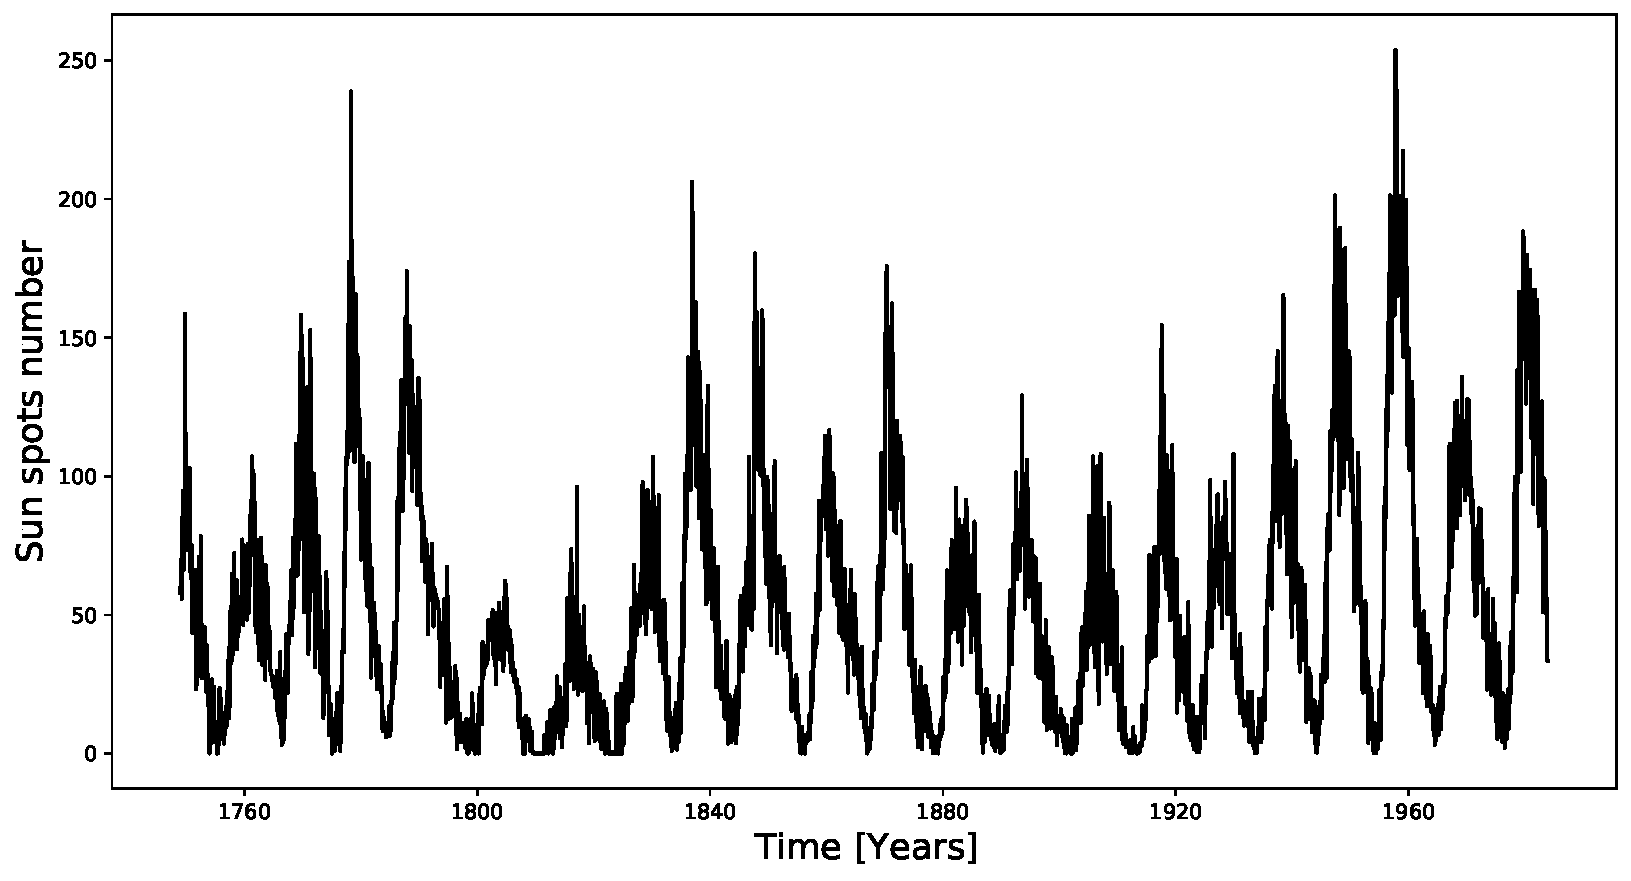
\includegraphics[scale = .45]{Images/SunSpots/SunSpotsNumbers.pdf}
    \caption{Monthly number of solar spots.}
    \label{fig:sunSpotsPlot}
\end{figure}
Fig \ref{fig:sunSpotsPlot} shows the monthly time series of Zurich Sunspots Number in a time period from $1749$ until $1983$. The periodicity in the time series is eye catching. \\
We are going to estimate the time series spectrum as a means of capturing periodicity in our dataset, MESA is applied with the FPE chosen as optimizer.  
\begin{figure}
    \centering
    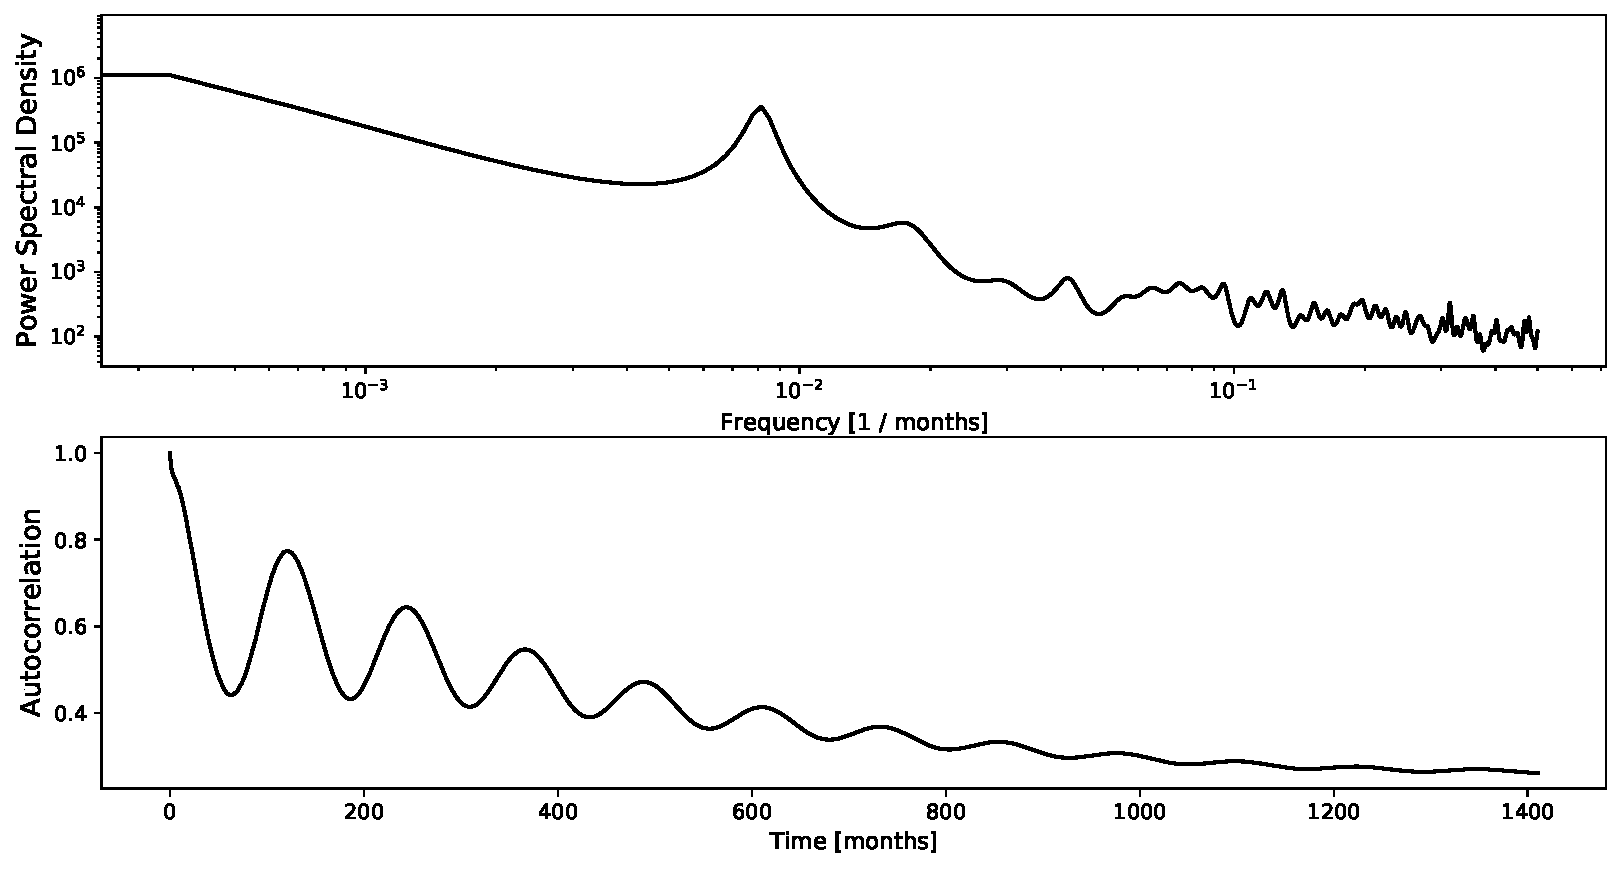
\includegraphics[scale = .45]{Images/SunSpots/SunSpotsPSD&ACR.pdf}
    \caption{Top panel: power spectral density for Zurich Monthly Number of Sun spots. Bottom panel: reconstructed autocorrelation function.}
    \label{fig:sunSpotsPSD&ACR}
\end{figure}
Figure \ref{fig:sunSpotsPSD&ACR} (bottom panel) shows the the autocorrelation function. It is a slowly decaying function of time whose peaks are located at multiples of 121 months (around 10 years), reproducing the periodicity of the sample. A slowly decaying function is a sign of the process to be long range.  
Figure \ref{fig:sunSpotsPSD&ACR} (top panel) shows the frequency estimate of the Power Spectral Density obtained with MESA. The 0 frequency component is different from zero, indicating that the mean of the process is different from zero. 
There is evidence of some well defined periodicity at some frequency $f_0$, superimposed to some $f^{-\alpha}$ noise, both $f_0$ and $\alpha$ to be determined. MESA is also able to capture secondary peaks, at frequencies that are multiple of the fundamental frequency.  \\
To study it, we consider the power spectral density as a superimposition of colored noise and a Cauchy resonance. A fit of PSD background, see the top panel in Figure \ref{fig:SunSpotsFit}, shows that the decreasing component of the power spectral density can be actually treated as colored noise of the form:
\begin{equation}
    f_{noise} = (1.1 \pm .2) f^{-1.74 \pm 0.03}
\end{equation}
\begin{figure}
    \centering
    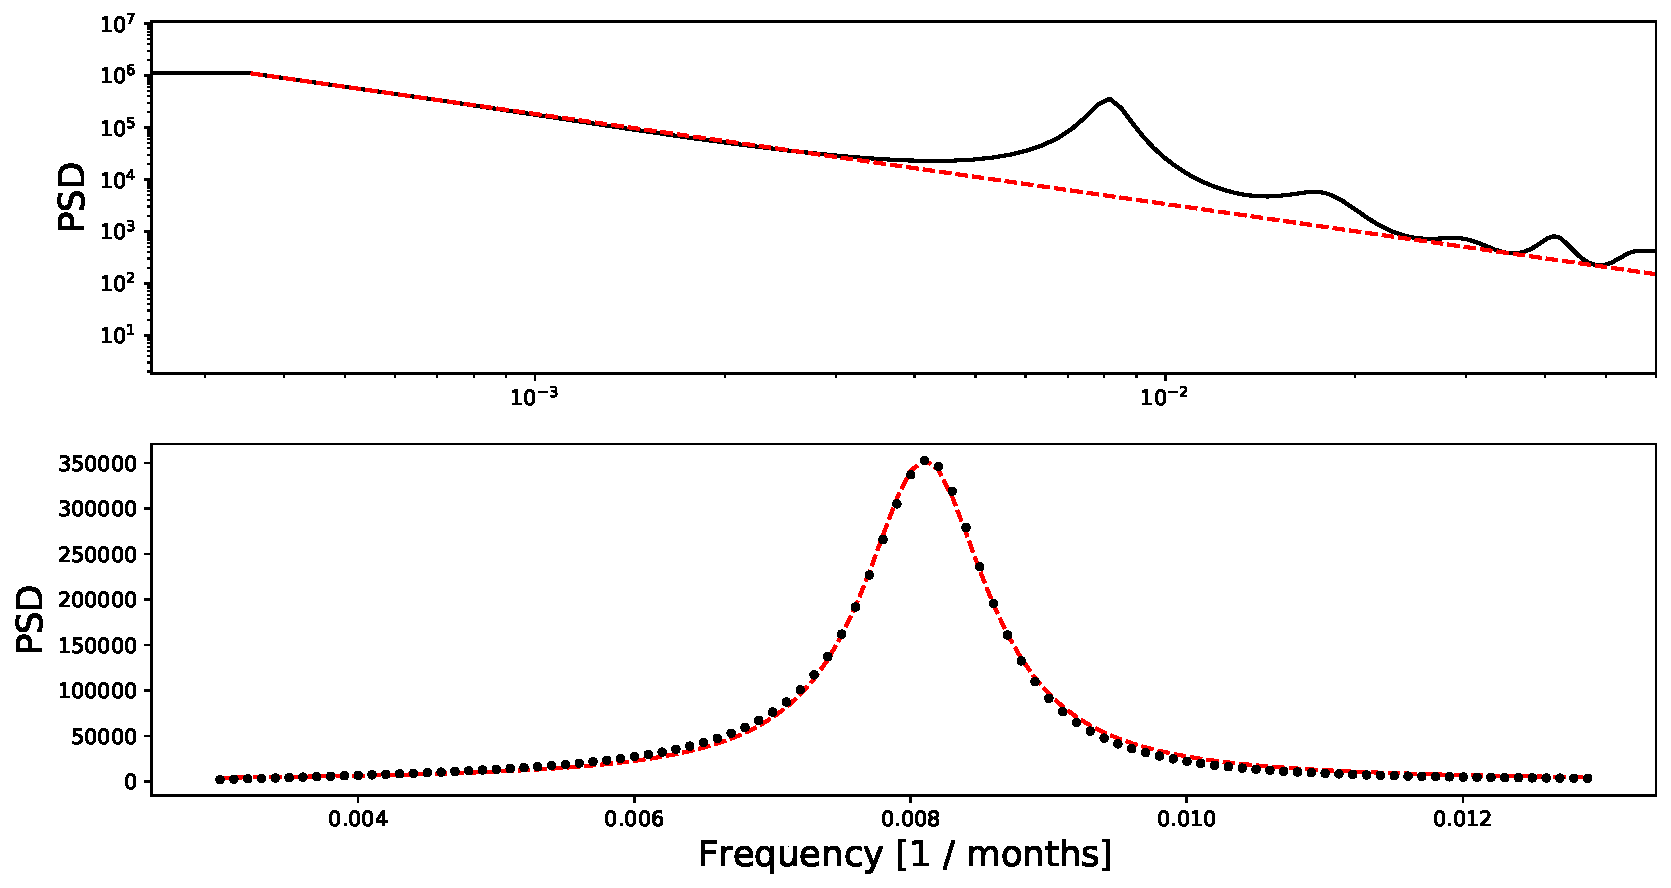
\includegraphics[scale = .45]{Images/SunSpots/SunSpotsFit.pdf}
    \caption{Power spectral density against fitting of background with colored noise (top) and with a Cauchy distribution (bottom).}
    \label{fig:SunSpotsFit}
\end{figure}

In this way, the non periodic component can be eliminated from the spectrum and the peak can be fit. Even if not perfectly symmetrical, we chose a Cauchy distribution to fit the peak (Figure \ref{fig:SunSpotsFit}, below), parameterized as 
\begin{equation}
    C(f) = \frac{\hat{h} }{1 +\left( \frac{f - \hat f_0}{\hat \gamma}\right)^2}.
\end{equation}
The fit provided for the parameters the following values
\begin{equation}
    \nonumber 
    \hat h = (3.35 \pm 0.02)\cdot 10^5; \quad 
    \hat f_0 = (8.104 \pm 0.003) \cdot 10^{-3} \mbox{months}^{-1}; \quad 
    \hat \gamma = (5.49 \pm 0.05) \cdot 10^{-4} \mbox{months}^{-1}
\end{equation}
and the periodicity in Sun spots is found to be 
\begin{equation*}
    10.28 \pm 0.05 y_{ears}.
\end{equation*}
It is interesting to understand the meaning of the parameters by taking an inverse Fourier Transform, the autocorrelation correspondent to a pure Cauchy shaped PSD is:
\begin{equation}
    K \gamma e^{-\gamma \vert t \vert } e^{-\imath f_0 t}.
\end{equation}
$f_0$ is the natural frequency of the oscillating component for the power spectrum, while $\gamma$ is the inverse of a lifetime $\gamma = \frac{1}{\tau}$ and can be taken as a typical time scale for the autocorrelation of the periodic component, but this is not true for the whole dataset since its power spectral density is, at first approximation, the sum of the two components. Since they do not provide additional information, secondary peaks (Figure \ref{fig:sunSpotsPSD&ACR}) have been neglected.

\begin{figure}
    \centering
    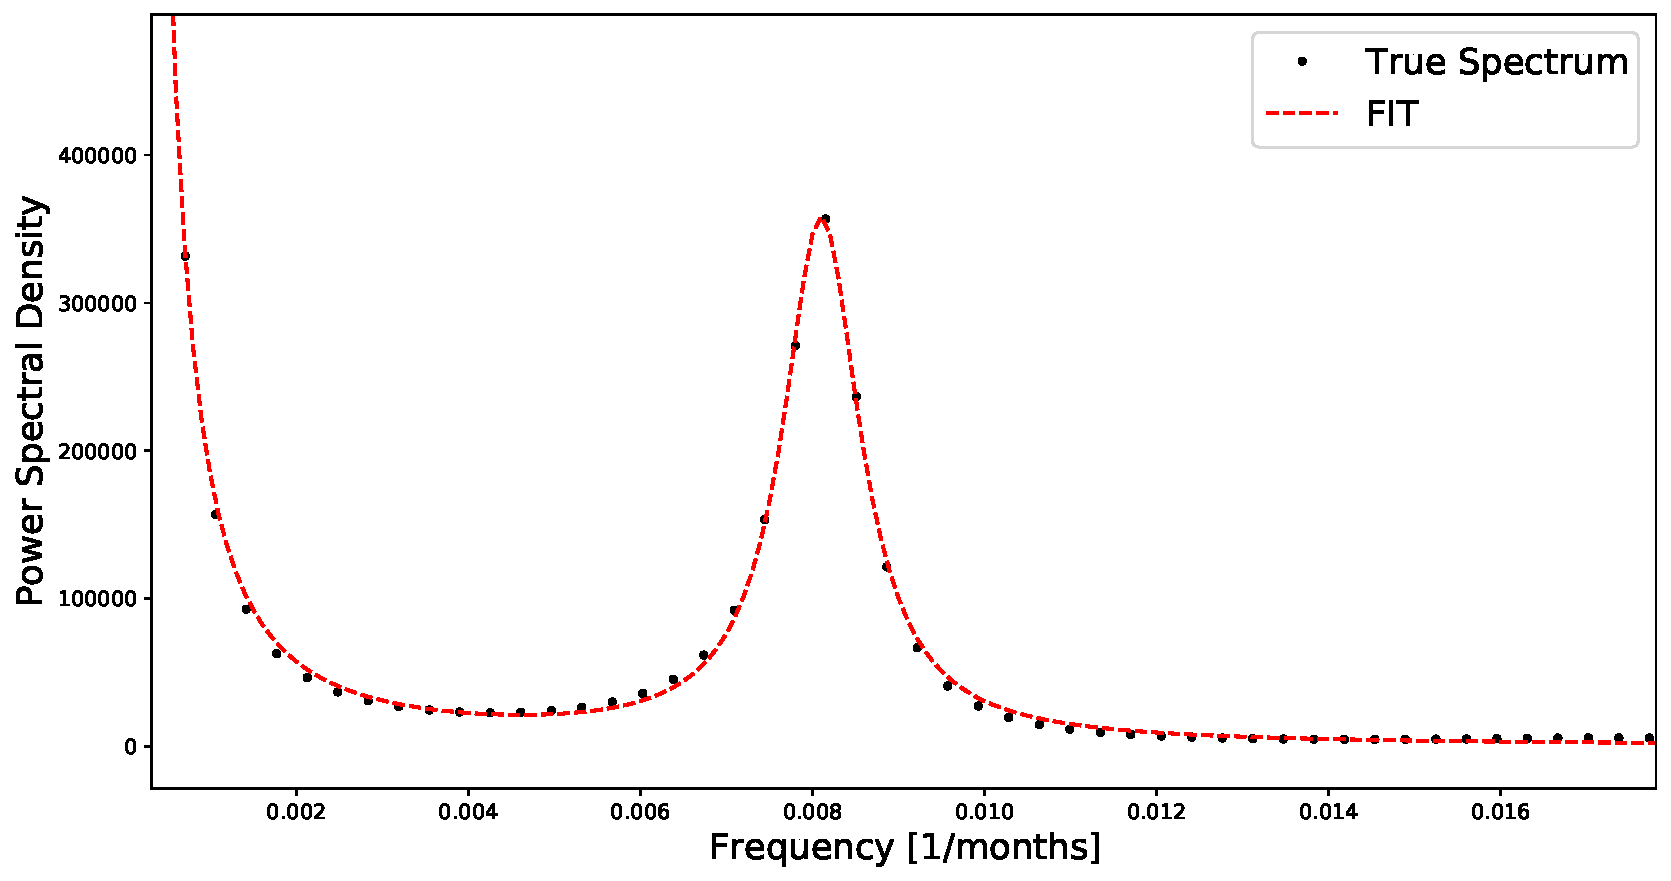
\includegraphics[scale = .47]{Images/SunSpots/SunSpotsTotalFit.pdf}
    \caption{Fits to the spectrum considered with two components, one $f$ noise component and one Cauchy component for the resonance.}
    \label{fig:PSDendFit}
\end{figure}
Figure \ref{fig:PSDendFit} shows the fit obtained adding the $f$ noise component with a Cauchy resonance. The result is accurate enough to describe the main component of the power spectral density: having neglected secondary peaks does not affect the computation of the quantity of interest. 

\section{Time Series Forcasting}
With MESA we have been able to compute a smooth and high quality power spectral density for the time series of Sun spots, estimating the period of solar activity to be $  10.28 \pm 0.05 y_{ears}$. This is just a first result of the application of MESA. On the other hand, the computation of the prediction error filter allows us to predict the future values for our observations as well as their credibility regions. Since we want to compare the results of the forecast with real data, we apply MESA again on our dataset, excluding the 200 last data points. We will then compare the excised data with the predictions of MESA. Having computed the prediction error filter from the data, eliminating the first value (which is one) and changing the sign to the remaining, we have an estimate of the autoregressive coefficients. In this way, The process is estimated to be an $AR(96)$ process.
\begin{figure}
    \centering
    \includegraphics[scale = .47]{Images/SunSpots/SunSpotsARcoefficients.pdf}
    \caption{Estimate of the autoregressive coefficients for Sun Spots time series.}
    \label{fig:SunSpotsFilter}
\end{figure}
Figure \ref{fig:SunSpotsFilter} shows estimate for the autoregressive coefficient of the time series. 
The behaviour of the coefficient as a function of the length is characteristic, the dependence is different from zero and positive for only few values, and becomes a noisy fluctuation around $0$ of both positive and negative components after few observations. The standard deviation $\sqrt{P_N}$ of the superimposed white noise is estimated to be $\sqrt{P_N} = 14.77$. Having computed the filter and variance for the $AR$ predictor, new values can be inferred by
\begin{equation}
    x_t = \sum_{i = 1}^{96}a_i x_{t-i} + \nu_t \text{ with } \nu_t \sim \mathbf{N}(0, \sqrt{P_N}).
\end{equation}
In every step of the prediction, the deterministic component has to be summed to the white noise component. Since the process is linearly dependent on its previous values, this random component will propagate in the time series. For this reason, in forecasting it makes no sense to consider a realization only: even if a single prediction is an admissible realization for the process, taken alone it has no statistical meaning. \\
For this reason, to have a fair comparison between simulated and observed realization, we will simulate 3000 series of 200 points each. \\ 
Since random error propagates in the time series, we expect our prediction to be a consistent estimate of the observed time series for a number of points shorter than filter's length. In this interval, in fact, both simulation and real data are still dependent on the observed data. For predictions of length comparable with AR order or longer, our prediction is based on simulated data only and can be largely different from the observed series.
\begin{figure}
    \centering
    \includegraphics[scale = .47]{Images/SunSpots/SunSpotsForecast.pdf}
    \caption{Forecasting on Sun spots time series using MESA linear predictor. Observed time series is compared with ensemble mean and 95\% Cr.}
    \label{fig:SunSpotsForecast}
\end{figure}
Figure \ref{fig:SunSpotsForecast} shows the numerical prediction of MESA (red dashed line), computed as a mean over the ensemble, and the future values assumed by the series (black solid line) for 200 months, credibility regions at 95\% are also reported. \\ 
The vertical line at an abscissa of $96$ provides a visual separation between a time interval shorter and longer than the autoregressive order for the process. Is evident that this line separates two different regimes for the estimate. At earlier times, our inference is almost everywhere consistent with the observed data, and they are everywhere comprised in the $95\%$ regions. \\ 
At later times, the quality of inference is degraded, because the inference in this region is no more dependent on observed data. Even if the credible regions become larger there are some values laying outside them. Secondly, the observed data are no more consistent with the estimate obtained from the mean. \\
The only information we can achieve in this area is about the increasing / decreasing trend of the series. This happens because this trend is determined by the deterministic component of the process. \\ 
So, we conclude that a proper inference with MESA can be obtained for a time period shorter than the length of the filter, in that case a period of $70\sim 80 months$, i.e. around $6$ years, which is a remarkable result. \\ 
It is important to stress a fact: to obtain all the results, we assumed no knowledge on the process itself. To study power spectral density, gain quantitative information and make high quality forecast, we did not assume any physical model. All we obtained was directly contained in the data themselves and MESA extracted as much information as possible. This shows how the PSD - Autorgressive duality is powerful. With the support of Wold's theorem, given a stationary process, MESA is a tool that allow to find an approximate description of its ARMA(p,q) dual without making any assumption on the process.

\section{Conclusions}
In this section we applied MESA to a first simple dataset: the number of Sun spots. Even if simple, this dataset makes clear some important features of the method. \\ Firstly, we have been able to estimate accurately the power spectral density of the process. We have seen that, at least at the leading order, it can be treated as the sum of a colored noise component and a periodic component, described by a Cauchy resonance. The f noise component has an exponential decay with exponent $\alpha = -1.74 \pm 0.03 $ . 
The periodic component is associated to a frequency
\begin{equation}
    \nonumber 
    \hat f_0 = \left(8.104 \pm 0.003 \right) \cdot 10^{-3}. months^{-1}
\end{equation}
Secondly, we worked out with the autoregressive duality computing its AR coefficient from the prediction error filter. The AR process is found to be well approximated by an $AR(96)$ process. Having computed the coefficients, we showed how MESA can be used to  forecast over a time period shorter than the AR order $p$. This is because in that range, our estimate depends on both observed and simulated data. With no knowledge at all on the physics behind the process, we have been able to perform accurate inference and predictions with the only application of MESA. This is a very remarkable result and shows how MAXENT provide a powerful tool to make inference without superimposing any model to the dataset. 

\newpage 
\chapter{Sinusoidal Signals}
\section{Introduction}
The estimation of parameters describing theoretical models is one of the key point in statistical Analysis. Considering some dataset and model, dependent on a set of parameters $\vec \theta$, the objective is to find the values for $\vec \theta$ that better describe the observation. \\
Such an estimate can only be performed if noise is correctly characterized, otherwise the inference might be imprecise.  Since data come out as a superposition of signal and noise, the characterization of noise is often made 'off-source', i.e. studied in a time window of proper length that precedes the stretch of data containing the signal. Such an analysis assumes the noise to be stationary for a period of time and is seldom justified. In this chapter, we explore a novel idea that allows to perform an "on-source" characterization of noise by the use of MESA. After a short explanation of the basic idea, we will apply this new method to a toy problem of sinusoidal signal superimposed with colored noise. 
\section{Bayesian inference}
\subsection{Bayes Theorem}
Bayes theorem is the fundamental tool for Bayesian inference. \\ 
Let $\vec \theta \in \mathbb{R}^N$ be the set of parameters we want to infer. The objective in Bayesian Analysis is the computation of the posterior distribution for the parameters given some data $D$, prior information $I$ and model $M$. \\ 
Starting from Bayes theorem, the goal is to determine the distribution $P(\vec \theta \vert D M I)$ such that 
\begin{equation}\label{eq:Bayes}
    P(\vec \theta \vert D M I) = \frac{p(D\vert \vec \theta M I)}{p(D \vert M I )} p(\vec \theta \vert M I) 
\end{equation}
holds. \\ 
The posterior on the left hand side indicates how the parameters are distributed according to the model, prior information and the observation of some data $D$. \\ 
On the right hand side $p(\vec \theta \vert M I)$ is the prior distribution for the parameters given only model and prior information, while $p(D \vert \vec \theta M I)$ is the Likelihood. The quantity in the denominator $p(D\vert M I)$ is a purely Bayesian quantity called evidence. For sake of simplicity, since we are not going to use it explicitly, being computed as
\begin{equation} 
    p(D \vert M I) = \int d\vec \theta p(D \vert \vec \theta M I) p(\vec \theta \vert M I),
\end{equation}
we can consider it as a normalization factor. \\ It is clear that, to perform Bayesian inference,
we need to correctly determine the previous quantities. \\ 
Concerning the prior distribution, MAXENT provides a way to assign them, but there are several more methods and a huge literature about it \cite{jaynes2003ptl}. \\ 
\subsubsection{Assigning Likelihood}
Our main interest is the determination of the likelihood from the information and a Model $M$. \\
The Model $M$ defines functional relations between physical quantities, dependent on the set of parameters $\vec \theta$. Given some value $x$ for a variable, the model $M$ allows us to determine the value of a causally related variable $z$, via 
\begin{equation}
    \nonumber 
    \vec z = M(\vec x \vert \vec \theta).
\end{equation}
The previous relations are our physical laws that we want to test and the determination of the parameters is a fundamental task to assert the validity of some Model or theory. In general, we do not observes pairs of values $(z_i, x_i)$, but we have to deal with some error that can mask the deterministic relation between the two. Out data will be "couples" of points of the form 
\begin{equation}
    D = (y_i, x_i),
\end{equation}
where $y_i$ is determined from the model $M$ and some error $e_i$, via 
\begin{equation}
    y_i = z_i + e_i .
\end{equation}
In general, each of the previous quantities, the observation $y_i$, the prediction from the model $z_i$ and the error $y_i$ will have their own probability distributions. The Likelihood can be obtained marginalizing the joint probability distribution over $z_i$ and $e_i$, assuming them to be independent: 
\begin{align}\nonumber 
    p_y(y_i \vert M \vec \theta I) &= \int de_i dz_i p(y_i, z_i, e_i \vert M \vec \theta I) = \int de_i dz_i p_y(y_i \vert z_i e_i M \vec \theta I) p_z(z_i \vert M \vec \theta I) p_e(e_i \vert M \vec \theta I)
\end{align}
Since $y_i$ is uniquely determined from the model prediction $z_i$ and the error $e_i$, its conditional distribution is 
\begin{equation}\nonumber 
    p(y_i \vert z_i e_i M \vec \theta I) = \delta(y_i - z_i - e_i),
\end{equation}
so that 
\begin{align}\nonumber 
    p_y(y_i \vert M \vec \theta I) &= \int de_i dz_i \delta(y_i - z_i - e_i) p_z(z_i \vert M \vec \theta I) p_e(e_i \vert M \vec \theta I )\\ \nonumber 
    &= \int dz_i p_z(z_i \vert M \vec \theta I) p_e((y_i - z_i) \vert M \vec \theta I) 
\end{align}
that is the convolution between the distribution of the model and the distribution for the error. For a deterministic model, such that $z_i = m(x_i \vec \theta)$ is uniquely determined, the previous can be furhter simplified 
\begin{align}
    p(y_i \vert M \vec \theta I) &= \int dz_i \delta\left(z_i - m(x_i \vert \vec \theta)\right) p_e\left((y_i - z_i) \vert M \vec \theta I\right) \\ \nonumber 
    & = p_e\left((y_i - m(x_i\vert \vec \theta)) \vert M \vec \theta I\right)
\end{align}
and for such a model the likelihood is uniquely determined from the distribution of the errors. For independent data $y_i$ and errors $e_i$, given a set of observations, the Likelihood can be rewritten as
\begin{equation}
    p(\vec y \vert M \vec \theta I) = \prod_{i}p_e\left(y_i - m(x_i \vert \vec \theta) \vert M \vec \theta I \right).
\end{equation}
Given some deterministic model $M$, the Likelihood is uniquely determined by the distribution of the errors,
so that a full characterization of the error is a necessary step to compute the posterior for the distribution. \\ 
\newpage
\section{Power Spectral density Computation}
From the previous discussion, the role of power spectral density in parameter estimation appears to be clear: Parameter estimation can only be done if an estimate for the variance of the noise is given. \\
We briefly review how this is done for signals and propose a new 'on-source' method based on MAXENT. 
\subsection{Pure noise signals} 
Computation of power spectral density for pure noise signals of the form
\begin{equation}
    y(t) = n(t)
\end{equation}
is the easiest task, since our observation is coincident with noise only and we don't have to extract it from the data. Also if simple, this is the very start to study even more complex data that are a superposition of signal and noise. 
The most traditional approach is based on Bayes theorem.
We can consider noise to be normally distributed with 0 mean and with some variance to be determined. To infer on the posterior distribution, a prior distribution for $\sigma$ have to be assigned
\begin{equation}
    \nonumber
    p(\sigma \vert D I) = \frac{p(D \vert \sigma D I)}{p(D \vert I)}p(\sigma \vert I).
\end{equation}
Firstly, we need to rewrite the previous in Frequency domain with discrete time sampling. Under these conditions, the so-called Whittle Likelihood \cite{Rover} provides a discretized version of a normal Likelihood in frequency Domain: 
\begin{equation}
    \label{eq:Whittle}
    -\frac{1}{2}\log L(\tilde n(f_i) \vert \vec S) = - \sum_{j = - N /2}^{N / 2}\left(\log(S(f_j) +  \frac{\frac{\Delta_t}{N}\vert \tilde \tilde n \vert ^2}{S(f_j)} \right), 
\end{equation}
being $\tilde n$ the Fourier Transform of noise. In this domain, a prior on Power Spectral Density has to be assigned also. In this way, the posterior on the power spectral density can be uniquely determined as 
\begin{equation}
    p(S(f) \vert D I ) = p(\tilde n \vert S I) p(S(f) \vert I) 
\end{equation}
This approach allows us to determine a posterior for the power spectral density and make an estimate with error bars. 
This easy example can become very complex in real cases, since the number of parameters can be arbitrarily large and a priori assignment for each of them is needed. \\
But, neglecting technicalities, such an approach is still possible. \\ 
It is interesting to see how MESA enters in this case. Having a realization of pure noise, the determination of power spectral density simply reduces to the application of MESA to the time series.
The disadvantage is that, with respect to Bayesian inference, we will only have an estimate for the power spectral density and no other quantities. The advantage is that in complicated cases, this estimate is model independent, and no assumption on noise behaviour are needed. Such a simple examples makes clear what are the main differences between MESA and model based approaches, both having their pro and cons depending on the case of study. 
\subsection{Off Source Estimate}
Even if pure noise signals are not in general our main goal, they provide a useful way to perform parameter estimation in case of data that are a superposition of both signal and noise:
\begin{equation}
\nonumber 
d(t) = z(t) + e(t).  
\end{equation}
In cases like this, the main objective is to compute the Posterior for the parameters $\vec \theta$ so that an estimate on their value $\vec \theta_0$ based on the observed Data can be performed. \\ 
Equation (\ref{eq:Bayes}) only formally solve this problem: to apply it, assigning likelihood is a necessary step and so posterior can be computed only after an estimate for power spectral density and noise characterization is needed. \\ 
One of the most common techniques for solving this problem is the "off source noise characterization" \cite{offsource}.
With off source studies, noise characterization is not made in the same time window where signal also lives. If signal duration is $T$, noise is studied in the $T$ seconds before signal detection. \\ 
In this way, our problem can be divided in two subsequent steps, the first one being the characterization of a pure noise signal and the second one being the estimate of parameters via Bayes theorem, that can be made with proper algorithms like MCMC.  \\
Off source characterization is an efficient and fast way to characterize noise and is very proficient when noise is stationary. 
But in the case of non stationary noise such an approach shouldn't be applied since it could bring to misleading and wrong results. 

\subsection{On-source Estimate}
Our objective is to propose an 'On-source' computation to characterize noise in the same time window where signal lives, to perform a better estimate of parameters in case of non stationary noise. To avoid making assumptions on power spectral density shape, we will use MESA for its estimate and computation. This will allow us to reduce at a minimum the number of assumptions needed to perform the estimate. \\ 
We will explain our idea referring to Markov Chain Monte Carlo (MCMC) algorithm. 
\subsubsection{The Idea in a nutshell}
The conceptual simplicity of this class of algorithms is ideal to explain the idea of on source estimate without introducing blinding technicalities.  \\ 
Given some observations $D(t)$ described with some model $M(\vec \theta)$, MCMC algorithm allow to sample parameters space to find the maximum of posterior distribution for the parameters $\vec \theta$. \\
Let N be the number of recursion for the algorithm, and suppose Likelihood and prior are assigned. The structure of MCMC for posterior sampling is the following:

\begin{enumerate}
    \item Set $N = N_0$; 
    \item Set $i = 0$; 
    \item Randomly samples $\vec \theta_i$ values from prior; 
    \item Compute value for Posterior on samples $\vec \theta_i$
    \begin{equation*}
        P_i = P(\vec \theta = \vec \theta_i \vert D M) = p(D \vert \vec \theta_i M) * p(\vec \theta_i \vert M) 
    \end{equation*}
    \item Update parameters $\theta_i$
    \begin{equation}\nonumber 
        \vec \theta_{k} = \vec \theta_i + \vec \epsilon_i \qquad \text{with: } \vec \epsilon_i \sim D(0, \vec \sigma) 
    \end{equation}
    \item Compute $P_k$
    \item If: 
        \begin{enumerate}
            \item $P_k \geq P_i$: Set $\vec \theta_{i+1} = \vec \theta_{k}$
            \item $P_k < P_i$, Set: \\ 
            $\vec \theta_{i + 1}= \theta_k$ with probability $\frac{P_k}{P_i}$ or \\ $\vec \theta_{i+1} = \theta_i$ with probability $1 - \frac{P_k}{P_i}$
        \end{enumerate}
    \item if $i = N_0$: end
    \item increment $i \rightarrow i + 1$ 
    \item back to step 5. 
\end{enumerate}
With such an algorithm one can produce an arbitrary number of samples representative of the peak for the posterior distribution. \\ 
If the power spectral density is given, it has to be used to compute the posterior value. What happens if we don't know it? \\ 
The simplest approach is considering it as a parameter and infer it simply sampling a larger posterior distribution of the kind: 
\begin{equation}\nonumber 
    P(S_1, \dots, S_{N}, \theta_1, \dots, \theta_N \vert D M I). 
\end{equation}
This would require the introduction of a prior distribution for every component of the PSD. Conceptually it is a practicable approach, but for large data set of $N$ points one should infer $N / 2$ values for the power spectral density, and complexity would increase accordingly. \\
Our objective is to propose a different approach based on MAXENT. At first, we note that at step $(6)$ the computation of the Posterior implies that we are computing the quantity: 
\begin{equation}\nonumber 
    d(t) - z_i(t),  
\end{equation}
with $z_i$ the model computed on the current values $\vec \theta_i$ for the parameters. 
Collaterally, an estimate of the noise $n_i(t) = d(t) - z_i(t)$ is provided as a function of the current value for the parameters. \\ 
Having a sample of possible realization for noise, the basic idea is to compute $z_i$ power spectral density with MESA and use this estimate in the evaluation of the posterior.  \\ 
The modification needed in the algorithm to insert the computation of PSD is very simple, and can be resumed as follows: 
\begin{enumerate}
    \item Set $N = N_0$; 
    \item Set $i = 0$; 
    \item Randomly samples $\vec \theta_i$ values from prior; 
    \item Compute noise as $n_i = d - z_i$
    \item Compute power spectral density $S_i$ applying MESA on $n_i$
    \item Compute value for Posterior on samples $\vec \theta_i$ and $S_i$
    \begin{equation*}
        P_i = P(\vec \theta = \vec \theta_i \vert D S_i M) = p(D \vert \vec \theta_i S_i M) * p(\vec \theta_i \vert M) 
    \end{equation*}
    \item Update parameters $\theta_i$
    \begin{equation}\nonumber 
        \vec \theta_{k} = \vec \theta_i + \vec \epsilon_i \qquad \text{with: } \vec \epsilon_i \sim D(0, \vec \sigma) 
    \end{equation}
    \item Compute noise as $n_k = d - z_k$
    \item Compute power spectral density $S_k$ applying MESA on $n_k$
    \item Compute $P_k$
    \item If: 
        \begin{enumerate}
            \item $P_k \geq P_i$: Set $\vec \theta_{i+1} = \vec \theta_{k}$
            \item $P_k < P_i$, Set: \\ 
            $\vec \theta_{i + 1}= \theta_k$ with probability $\frac{P_k}{P_i}$ or \\ $\vec \theta_{i+1} = \theta_i$ with probability $1 - \frac{P_k}{P_i}$
        \end{enumerate}
    \item if $i = N_0$: end
    \item increment $i \rightarrow i + 1$ 
    \item back to step 5. 
\end{enumerate}
This method has many great advantages. \\
Firstly, it doesn't require any assumption on prior for power spectral density and so minimizes the number of assumptions needed. \\ 
Secondly, we end up having a large number of samples for power spectral density also, and its posterior can be reconstructed. \\ 
The most important implication is that we can marginalize the posterior for the parameters with respect to the power spectral density, obtaining a conservative - model independent estimate of their distribution. \\ 
One objection could be raised at this point. 
We saw that MESA spectrum is analytical when stationary noise is considered, since it has no poles on the unitary circles where PSD is actually evaluated.  One could state that we are trying to abandon the too restrictive hypothesis for noise to be stationary, studying it with some method that requires is stationarity. \\ 
To answer this objection some specifications are needed, in fact, this statement is correct.
The assumption of stationarity is a simplifying assumption that allow us to study noise with very powerful tools. Our objective is not to completely relax this assumption, but to make it less restrictive. With off-source analysis, we are assuming noise to be "approximately stationary"  for a time period that is (at least) twice the duration of the signal. \\ 
On source analysis requires signal to be approximately stationary in the same time window where signal lives, that is a less stringent hypothesis. This also clarify the domain of application of this on-source method. If the typical time scale of significant changes of noise is larger than the duration of the signal, on-source parameters estimate with MESA might provide an efficient solution to the problem. If typical time scale are shorter or comparable with signal duration, this method cannot ensure to provide a correct estimate. 


\section{Sinusoidal Signal} 
As proof-of-principle we perform on-source study with the above method on two different time series: a sinusoidal signal with the superimposition of brown noise and a sinusoidal signal with a drift in the frequency, superimposed to noise generated from Ligo Power Spectral Density. For both its stability and fast computation, FPE is the ideal optimizer to perform this kind of analysis. 
Off-source estimate of the data will also be provided using Welch Method and Alternative CAT. Since noise is stationary, we expect the on-source method to provide an equivalent estimate on parameters. 
\subsection{Brown Noise}
As first step, we generate the sinusoidal signal 
\begin{equation}
    a_1 \sin(2\pi f t) + a_2 \cos(2\pi f t)
\end{equation}
with values for amplitude and frequency parameters chosen to be
\begin{equation}\nonumber 
    a_1 = 5, a_2 = 7, f = 7.3. 
\end{equation}
The signal is superimposed with Brownian noise, whose PSD is 
\begin{equation}
    S(f) = \frac{3}{f^2 + 0.01}
\end{equation}
whit 0.01 inserted to avoid the divergence at f= 0. Figure (\ref{fig:BrownData}) represents the dataset we will analyze. First half of the data are a pure noise signal, while the second half a the superimposition of noise and sinusoidal signal with a signal to noise ratio (SNR) $\sim 37\%$

\begin{figure}
    \centering
    \includegraphics[scale = 0.40]{Images/BrownData/BrownData.pdf}
    \caption{Dataset under analysis. First half of the data are pure noise signal d(t) = n(t), needed to perform off-source characterization of noise, while the second half is the superposition of noise and sinusoidal signal d(t) = n(t) + z(t), that will be used to perform parameter estimation with both off-source/on-source methods}
    \label{fig:BrownData}
\end{figure}
This dataset is composed of 2000 points. The whole allow us to perform off-source analysis computing the power spectral density off noise in the first 1000 and parameter estimation with the second 1000. This second half will be the only one needed to perform on-source  analysis. The results of parameters estimation and PSD reconstruction will be then compared. 
\subsubsection{Off-source analysis}
As first step to perform off-source analysis, the reconstruction of the power spectral density is needed. Such an estimate is obtained with both Welch Method and Alternative CAT method. 
\begin{figure}
    \centering
    \includegraphics[scale = .40]{Images/BrownData/OffSource_PSDcomparison.pdf}
    \caption{Comparison of true power spectral density with estimate obtained with Welch method (green) and Alternative CAT (red). Alternative CAT estimate is made on sub arrays of 100 points with a 50\% superimposition}
    \label{fig:brownPSD_offSource}
\end{figure}
Figure \ref{fig:brownPSD_offSource} compares the estimate of the power spectral density obtained with Welch Method (green) and Alternative Cat (Red).
Both of the estimates are representative for the power spectral density, but aCAT minimizes the variance of the result. The parameter estimation is obtained with the MCMC sampling of a Nested Sampling 
Algorithm \cite{Skilling..735..395S} \cite{john_veitch_2020_4109277}. 
Figures (\ref{fig:BrownCATposterior})shows the posterior for the parameters computed on alternative CAT (above) and Welch  (below) power spectral densities 
\begin{figure}
    \centering
    \includegraphics[scale = .47]{Images/BrownData/BrownOffPosteriors.pdf}
    \caption{Posterior distributions for the parameters obtained using alternative CAT (above) and Welch (below).}
    \label{fig:BrownCATposterior}
\end{figure}
The estimate for the parameters with Welch's
is 
\begin{equation}\nonumber 
    \hat a_{1; Welch} = 4.86 \pm 0.04 ; \quad \hat a_{2;  Welch} = 7.10 \pm 0.05 \quad \hat f_{Welch} = 7.30000 \pm 4 \cdot 10^{-5}
\end{equation}
The frequency estimate is unbiased and with a small error. The estimate for the second amplitude $a2$ lays in one standard deviation from the mean, while for the 1st amplitude parameter the real value is found to lay in 3.5 standard deviation. The results obtained with alternative CAT are more accurate 
\begin{equation}
    \hat a_{1; aCAT} = 4.94 \pm 0.07 ;\quad 
    \hat a_{2; aCAT} = 6.96 \pm 0.06;\quad 
    \hat f_{aCAT} =  7.30000 \pm 0.00005
\end{equation}
and a correct estimate for the parameters, since their true values are always comprised in one standard deviation from the mean. In similar cases where noise is stationary, the off-source approach can give results that are consistent with the real values for a signal. 
\subsubsection{On-Source Analysis}
On source estimate is performed directly on the dataset, so in the second half part of the data in figure \ref{fig:BrownData}, and the posterior sampling is obtained via the same Nested sampling algorithm used before. 
\begin{figure}
    \centering
    \includegraphics[scale = .47]{Images/BrownData/BrownOnPosteriors.pdf}
    \caption{Posterior distribution for the parameters obtained as on-source estimate}
    \label{fig:brownOnPosterior}
\end{figure}
Figure (\ref{fig:brownOnPosterior}) shows the posterior distribution for the parameters obtained with the on source estimate. With respect to the posteriors obtained with the off-source estimate, the domain is larger and so is the error in the estimate. the larger support for the posterior in the on source case is due to the fact that the power spectral density is not 'a priori' known, but evaluated step by step with the parameters. The uncertainty on the posterior affect the parameter estimation, resulting in larger posterior distributions. The estimate for the parameters obtained with on-source analysis is 
\begin{equation}\label{brownONestimate}
    \hat a_1 = 5.0 \pm 0.2 ; 
    \quad \hat a_2 = 7.0 \pm 0.4;
    \quad f = 7.3000 \pm 0.0001 
\end{equation}
Remarkably, the estimate results to be unbiased for every parameter, concerning the standard deviation it result to be one order of magnitude larger than that obtained with the off-source estimate.\newline
\begin{figure}
    \centering
    \includegraphics[scale = .43]{Images/BrownData/On_Source_PSDposterior.pdf}
    \caption{On-source reconstructed posterior with 90\% credibility regions. FPE estimate on real error is also reported. }
    \label{fig:brownOnSourcePSD}
\end{figure}Figure (\ref{fig:brownOnSourcePSD}) show the on-source estimate for the power spectral density obtain with $90\%$ Credbility regions. FPE estimate on the real Error is also reported. The estimate is computed taking the median over all the reconstruction obtained in the Monte Carlo. Median is chosen over the mean to be more representative for its greater stability.  \\ 
The true power spectral density is not consistent with the median of the ensemble, neither comprised in the $90\%$ Credibility. But it also has to be noticed that the median on-source estimate is almost coincident with the FPE estimate for the power spectral density, that is computed on the real error. This fact allow us to state that the off-set in the estimate is due to MESA and not to on-source estimate. The fact that the estimate of PSD on real error is coincident with our estimate is rather a good result, and the estimate of noise stress this fact. 
\begin{figure}
    \centering
    \includegraphics[scale = .43]{Images/BrownData/OnSource_ReconstructedNoise.pdf}
    \caption{'On-source' estimate of noise}
    \label{fig:brownNoise}
\end{figure}
Figure (\ref{fig:brownNoise}) compares the real error (black) with its estimate (red crosses). This estimate is computed taking the median of the errors over all the possible models reconstructed with MCMC algorithm.  The agreement is impressive and gives even more evidence that the disagreement between real PSD and the reconstruction is due to MESA only. This is easily understood comparing MESA analytical solution with the functional form we used to generate noise. Neglecting constants, we are requiring 
\begin{equation}\nonumber 
    \nonumber 
    \biggr \vert\sum_{i = 0}^p a_i e^{- \imath 2 \pi f i \Delta t}\biggr \vert ^2 \sim f^2. 
\end{equation}
The expansion on the left hand side could be consistent with $f$ if long orders are selected. In general $f^{-2}$ noise is brownian motion spectrum, that is an $AR(1)$ non-stationary process.  Under these assumptions we are working outside the limits of MESA, and so we are not ensured that we will obtain a consistent estimate. In fact, a check on the autoregressive coefficient shows that the filter obtained with FPE is of order 3, too short to be an accurate approximation. It interesting to note that the estimate obtained with alternative CAT method in the previous section, shown in figure \ref{fig:brownPSD_offSource}, is a way more accurate estimate for the power spectral density. Reminding that CAT chooses long filters, it is more able to capture the power low behaviour of the power spectral density, and the variance of the estimate is reduced taking the average over different realizations. All these facts underline that the non consistent estimate for the power spectral density is not to be considered as a failure of our proposal for on-source estimates.
\newpage 
\section{Ligo Noise}
The same analysis will be repeated on a sinusoidal signal with a linear drift $f'$ in the frequencies 
\begin{equation}
    z(t) = a_1 \sin\left(2 \pi (f + f' t) t\right) + a_2 \cos\left(2\pi(f + f' t)t \right), 
\end{equation}
whose parameters are valued 
\begin{equation}\nonumber 
    a_1 = 10^{-21}; \quad a_2 = 5\cdot 10^{-22}; \quad f = 128, \quad f' = 1.4 
\end{equation}
the sampling interval and observation time are respectively 
\begin{equation*}
    dt = \frac{1}{2048}; \quad T = 8,
\end{equation*}
both parameters and sampling time expressed in arbitrary units. 
The signal is superimposed with some noise randomly generated from the Ligo Power Spectral Density studied in chapter 2. 
\begin{figure}
    \centering
    \includegraphics[scale = .43]{Images/LigoOnSource/ObservedData.pdf}
    \caption{Simulated dataset used to perform the analysis}
    \label{fig:LigoData}
\end{figure}
Figure \ref{fig:LigoData} shows the dataset used for both 'off-source' and 'on-source' analysis. As a main difference from the previous case, the amplitude for noise is much greater than the amplitude of the signal. \\ 
The first 4 seconds of observation are pure noise, while the second are a superimposition of the deterministic signal $z(t)$ and noise $n(t)$. Again, the first 4 seconds will be used to study the power spectral density with the off-source estimate, while the last 4 seconds to perform parameter estimation. For these last for second SNR is reduced to $\sim 10^{-3}$. 
\subsection{Off-Source Analysis}
The off source analysis is performed characterizing noise with the alternative CAT approach and Welch approach. The reconstruction of the power spectral densities with the above methods is reported in figure \ref{fig:offPSDLigo}. 
\begin{figure}
    \centering
    \includegraphics[scale = .43]{Images/LigoOnSource/offPSDcomparison.pdf}
    \caption{Comparison of the estimate of the power spectral density obtained with Alternative CAT (red line) and Welch method (green line)}
    \label{fig:offPSDLigo}
\end{figure}
Both peaks are recognized but not perfectly characterized, especially the first peak's height is underestimated. Still, alternative CAT's estimate shows improved variance with respect to Welch's method. A comparison of the posterior for the parameters obtained with both methods is shown in figure (\ref{fig:posteriorLigoComparison}).
\begin{figure}
    \centering
    \includegraphics[scale = .46]{Images/LigoOnSource/PosteriorsComparison.pdf}
    \caption{Posteriors for the parameters of the model for both Alternative CAT (above) and Welch (Below)}
    \label{fig:posteriorLigoComparison}
\end{figure}
Alternative CAT results are peaked around the true results, while the posteriors obtained with Welch's method are slightly biased. The estimate for the parameters obtained with alternative CAT are found to be 
\begin{align*}
\centering
    \hat a_1 = (1.005 \pm 0.005) \cdot 10^{-21}; \quad 
    &\hat a_2 = (4.99 \pm 0.09) \cdot 10^{-22}; \\
    \hat f = 128.000 \pm 0.002; \quad 
    &\hat f' = 1.3998 \pm 0.0004, 
\end{align*}
so that the true values are always found to lay in one standard deviation from the mean. As can be seen from the posteriors, the estimate for the parameters obtained with Welch's method 
\begin{align*}
\centering
    \hat a_1 = (0.999 \pm 0.003) \cdot 10^{-21}; \quad 
    &\hat a_2 = (5.29 \pm 0.05) \cdot 10^{-22}; \\
    \hat f = 127.998 \pm 0.001; \quad 
    &\hat f' = 1.4004 \pm 0.0002
\end{align*}
gives less accurate results. The only parameters that lays in one standard deviation from the mean is the first amplitude parameter $a_1$. Both drift and frequency are correctly estimated in 2 standard deviations, that is a reasonable result, while for the second amplitude parameter (a2) the estimate is outside 3 standard deviations. The big variance of Welch's method in power spectral density estimate is
naturally affecting the estimate on the parameters, but still providing reasonable results, but the averaged MESA based results of CAT are way more accurate.  

\subsection{On-Source Analysis}
We now provide the result of the characterization of noise and the parameter estimate using the proposed on-source estimate. This case is of particular interest because signal noise ratio (SNR) is around $\sim 10^{-3}$, so that we are trying to characterize the dominant component of noise and separate it from a relatively weak signal.
Also in the study of brownian noise, even if SNR incredibly decreased, the result in the estimate is very accurate. 
\begin{figure}
    \centering
    \includegraphics[scale = .43]{Images/LigoOnSource/PArametersPosteriors.pdf}
    \caption{Posterior distribution for the parameters obtained with the on-source estimate}
    \label{fig:LigoOnPosteriors}
\end{figure}
Figure \ref{fig:LigoOnPosteriors} shows the posterior distribution computed for each parameter using the proposal method. Again the uncertainty on the estimate of the power spectral density propagates in the estimate for the parameters increasing the domain of the posterior and resulting in larger error bars. The estimate for each parameter is found to be
\begin{align}\label{LigoEstimate} 
    \hat a_1 = (1.00 \pm 0.01) \cdot 10^{-21}; \quad 
    &\hat f = 128.003 \pm, 0.004 \\ \nonumber 
    \hat a_2 = (4.7 \pm 0.2) \cdot 10^{-22} ; \quad 
    &\hat f' = 1.3993 \pm 0.0009
\end{align}
all the estimate but the second amplitude are very accurate and the true value lays inside the error defined by one standard deviation. For the second amplitude parameter the result is comprised in two standard deviation. \\ 
So, even for a weak signal we have been able to accurately resolve the deterministic signal described by the sinusoidal model. \\ 
But the added value of this new approach is the characterization of noise and the computation of its power spectral density. 
\begin{figure}
    \centering
    \includegraphics[scale = .43]{Images/LigoOnSource/PSDestimate.pdf}
    \caption{Estimate for the power spectral density obtained with the on-source analysis.}
    \label{fig:LOnSourcePSD}
\end{figure}
Figure \ref{fig:LOnSourcePSD} (above) shows the estimate for the power spectral density obtained with the on-source estimate, computed with FPE optimizer. The result of the estimate is accurate and representative of the real power spectral density. The credibility regions for the estimate are tight. This is probably due to the stability of FPE. We expect that for slightly small changes in the parameters the estimate for the power spectral density won't be largely affected. Since frequency and drift estimate are narrow, this is reflected on the posterior obtained for the power spectral density. This result is clearly related to the estimate and capability of the algorithm to discriminate between noise and signal. 
\begin{figure}
    \centering
    \includegraphics[scale = .43] {Images/LigoOnSource/ErrorEstimate.pdf}
    \caption{Comparison of the real noise (black dashed line) with the estimate obtained with the on-source analysis (red solid line)}
    \label{fig:LErrorEstim}
\end{figure}
Figure \ref{fig:LErrorEstim} shows the real error, superimposed to the data, and its estimate obtained with the on-source algorithm. This is computed as the ensemble median over all the reconstructed time series for the noise. The accuracy and precision in the reconstruction are incredibly high. The percentage error in the reconstruction of noise is found to be $r = 0.78 \%$, with a standard deviation $\sigma_r = 62.4\%$. The credibility regions are very tight, their average width is found to be $(3 \pm 1) \cdot 10^{-23}$, so that they are very narrow with respect to the values of noise time series, even though 100\% of the real values are found to lay between them. This explains why the accuracy in the reproduction is in one standard deviation around
$0.2 \% \div 2 \%$ and also the very tight credibility regions in the estimate for the power spectral density. \\ 
\begin{figure}
    \centering
    \includegraphics[scale = .43]{Images/LigoOnSource/NoiseEstimateBisect.pdf}
    \caption{Noise estimate VS real noise plot. The red dashed line represents the bisector of the axis}
    \label{fig:Bisector}
\end{figure}
To study the accuracy in the reproduction, the curve obtained in a "real error VS error estimate" is fitted with a straight line to see if the result is consistent with the bisector of the axis. Figure \ref{fig:Bisector} shows both the plot of the estimated error VS the real error and the bisector of the axis. 
The fit with a line 
\begin{equation}\nonumber 
    y = m x + q,
\end{equation}
gives as estimate for slope and intercept the following values 
\begin{equation}
    \hat m = 1.00000 \pm 0.00001; \quad \hat q = (0.02 \pm 1) \cdot 10^{-25},
\end{equation}
their functional relation is perfectly coincident with the bisector of the axis with an incredibly high precision, so that the small differences in the reproduction are probably statistically meaningless. 
With the on-source study parameters can be estimate with great accuracy, just renouncing to some precision in the result. Even for small values of SNR, this technique allow to distinguish between noise and signal in the data, reconstructing both in a very accurate way, just with the specification of the model for the signal.

\newpage 
\section{Conclusions}
In this chapter we briefly discussed the parameter estimate and the role played by the computation of power spectral density for noise to achieve this goal. Since likelihood distribution is uniquely determined from distribution of noise, a method to characterize this distribution is necessary. The standard off-source analysis requires to assume that noise is stationary for a time length that is at least twice the time of the observation of the signal. That assumption can lead to inaccurate parameter estimate when dealing with real noise, so that less restrictive one is needed. \\ For this reason, we proposed a new method to perform parameter estimation, introducing MAXENT computation of power spectral density in a MCMC algorithm. This means that only the strain of data where the signal live is needed. This new approach has been applied to two different 'toy models'. The first consists in a sinusoid with constant frequency, superimposed to some colored noise, with a SNR around $36 \%$. \\ 
In the second example we complicated the model by the introduction of a linear drift in the frequencies and superimposed with noise generated to be consistent with the Ligo power spectral density. In this second case, the signal noise ratio is reduced to $\sim 10^{-3}$. Comparing with the standard 'off-source' analysis, this new approach enlarges the error in the estimate of the parameters but lead to very accurate results: all the true values for the parameters have been recovered in no more than two standard deviations from the mean (eq: \ref{brownONestimate} and \ref{LigoEstimate}).  The real improvement regards the characterization of noise. Just using the strain of data where the signal actually lives, this approach has the capability to discriminate with huge accuracy which is the deterministic component of the data and which is simply noise, also for very low value of SN ratio. The estimate of noise (Figure \ref{fig:brownNoise} and \ref{fig:LErrorEstim}) is extremely accurate and precise: even if the credibility regions are very sharp, they always comprise the real values. Even the reconstruction of the power spectral density is extremely accurate, and most of the differences between the real power spectral density are attributable to MESA.  \\ 
Even if the aforementioned results are based on simple toy-models, the obtained results provide enough evidence that this method could refined to try an implementation on different, real, contexts. 

\newpage 
\chapter*{Conclusions and future developments}
In this thesis we introduced the maximum entropy principle (MAXENT) with some of its most relevant applications to the study of stationary time series. In chapter one MAXENT has been introduced and reformulated, according to the original work of Burg, to be applied in the estimate of power spectral densities. This method is known as 'Maximum Entropy Spectral Analysis' (MESA).   \\ 
Burg's approach admits a closed expression for the estimator of the power spectral density  in terms of some coefficients known as 'forward prediction error coefficients' (equation \ref{eq:MESApsd}). 
These $p$ coefficients provide a link between the spectral estimate and the characterization of the observed stochastic process. In fact, simply changing their sign, these new coefficient are a 'linear predictor' for the time series (equation \ref{eq:ARspectrum}). This means that they allow us to express the observed time series in terms of some autoregressive process of order $p$ (AR(p)). \\
Even more remarkably, the coefficients obtained with MESA are found to minimize the error in the prediction (equation \ref{eq:bestLinearPredictor}), i.e. their computation is equivalent to a least square fitting for the time series with an $AR(p)$ model. 
It is evident that importance of MESA goes far beyond his original domain of application: with no assumption on the physical model behind the observed data,  it accurately reconstructs the spectrum and characterizes the process..\\ 
Burg's algorithm is recursive and, for dataset whose autocorrelation function is not perfectly know, requires some criterion to estimate the recursive order. Different criteria to address this problem can be found in literature, and in chapter two we characterized three of them: Final Prediction Error (FPE), Criterion on Auoregressive Transfert function (CAT) and Optimum Bayes Decision rule (OBD).  The study considered the accuracy in the reproduction of two different spectra: a normal distribution and the a simplified spectrum of noise for the LIGO experiment (figure \ref{fig:LigoPSDOriginal}).  \\ 
The error in the reproduction resulted to be strongly dependent on the estimate of the recursive order $p$ (Figures \ref{fig:optcomparison} and \ref{fig:LigoOrderError}), and in both cases the estimate for $p$ associated with the smallest error is obtained with FPE. OBD lays in a region of shorter filter and larger error . The reconstructions obtained with these two methods are similar, but OBD provides estimates with a larger bias.  CAT, instead, shows a completely different behaviour. It selects larger orders than FPE,  but does not converge to any specific order. These long arrays are associated to a decreased bias in the estimate but with higher variance: it introduces a large number of spurious peaks in the reproduction. \\ 
For its peculiar properties, CAT's estimates might be improved averaging on various estimates obtained from subsets of the original dataset. The result will depend on both the length of the subsets and their overlapping. Short arrays (and so shorter filters) provide more biased results but less variance, while the opposite holds for longer arrays. For 'short' arrays the estimate is similar to the results obtained with FPE, but with lower accuracy. For longer arrays, it provides a similar result to the standard CAT but with reduced noise, so that this alternative approach makes sense if relatively ``long" arrays are chosen.  In chapter 4 this method is found to be way more accurate than $FPE$ (Figures (\ref{fig:brownPSD_offSource}) and (\ref{fig:brownOnSourcePSD})) in the reconstruction of power spectral density for Brown Noise. \\ 
In every application of this alternative method, the overlapping between the segments of data was fixed to $50\%$, so that a future perspective could be the characterization of the method for different lengths and overlapping.  \\ 
This modified approach has several cons. MESA is a powerful approach also because it is free of prior assumptions. The introduction of this alternative approach require some a priori choices on length and overlapping of sub segments of data that are hard to justify, we can only appeal to some 'expected behaviour' of the estimate with no general arguments supporting this choice. Also, it increases the complexity of the algorithm.  But the worst loss regards the link with autoregressive processes: taking the average, every information on the autoregressive coefficients is completely lost. \\ 
For both its accuracy and its stability, FPE has been chosen as the best optimizer to improve the estimate on the recursive order.\\ 
There are two other aspects that would deserve some studies. Firstly, for both spectra we investigated the estimate for fixed length of the time series.
Since $AR(p)$ processes are, for $p$ finite, just an approximation for the more general $ARMA(p,q)$ process, we expect the estimate for $p$ to be dependent on the length $N$ of the input time series. It would be interesting to see how and if the length of the estimate of recursive order is dependent on the original length of the time series $N$. \\ 
Secondly, since our interest was in characterizing noise, we studied the three optimizer focusing on power spectral density only. To achieve a full characterization of the criteria, one should generate an $AR(p)$ process with known coefficients and compare them with the estimates for length and values obtained with the three methods.\\ 
Finally, having characterized the three optimizer, in chapter 3 we applied MESA on a very simple time series: sun spots number. We obtained a description of the time series in terms of a AR(96) process. Fitting the spectrum (figure \ref{fig:sunSpotsPSD&ACR}) with some colored noise for the background and with a Cauchy resonance for the peak, we found a periodicity in the series of $10.28 \pm 0.05 years$. Knowing the forward prediction error, we have also been able to accurately predict the future values of the time series for $\sim 80$ months (figure \ref{fig:SunSpotsForecast}). \\
The last chapter developed a new proposal to perform 'on-source' bayesian parameter estimation, inserting MESA computation in a Markov Chain Monte Carlo algorithm (MCMC). With this approach, a model for the power spectral density is constructed "in real time" with the sampling for the parameters. In this way, with a relatively small number of assumptions, posterior samples are obtained for both the parameters of the model and the power spectral density. This proposal is convenient because, given some observed data $d(t) = z(t) + n(t)$, it allow us to separate the deterministic signal component $z(t)$ from the noise $n(t)$ directly 'on' the data. This approach allow us to relax the restrictive hypothesis on the stationarity for noise, that are usually required when noise is characterized 'off-source'. \\ 
This approach has been tested on a sinusoidal signal superimposed to brown noise and noise generated with the same LIGO Spectrum studied in the second chapter. We obtained very promising results. Concerning the estimate of parameters, we have great accuracy in the estimate (equations \ref{brownONestimate} and \ref{LigoEstimate}), with the loss of one order of magnitude in precision. This lost is probably related to the uncertainty in the estimate of the power spectral density. The most remarkable result is about the noise reconstruction from the data: the algorithm has been able to almost perfectly distinguish and separate noise and signal from the data (figures \ref{fig:brownNoise} and \ref{fig:LErrorEstim}). A linear least square fit of the estimated noise as a function of the real noise is found to be perfectly coincident with the bisector of the axis, up to a precision of $10^{-5}$, so that the differences between the real values for noise and its estimate are negligible from a statistical point of view.  \\ 
From the beginning, MESA have been applied to reproduce the simplified power spectral density of LIGO noise. The reason behind this choice concerns our future perspectives: the very next step will be the application of the new on-source method to public data of LIGO-Virgo collaboration, that will be a test bench for our analysis: the noise in the detector is not perfectly stationary as the one we generated in our simulation. But, since this analysis is also performed 'off-source', considering the results obtained with our toy models, it seems very reasonable to believe that the on-source method can be applied on gravitational waves data with optimum results. We are confident that we can be able to characterize almost exactly the noise component in the apparatus at the time the signal was caught. \\
The complete absence of assumptions on noise, makes this method a worth trying approach to several process. Special candidates are observations whose noise component cannot be completely understood and modeled. 
A simple example, reminiscent of our sinusoidal model, is the transit of exoplanets around a star. The partial eclipse due to the transit of the exoplanet in front of the star, will result in an observed luminosity that is periodic in time. This oscillatory, deterministic behaviour, will be superimposed to noise from various sources, such as stellar activity, the presence of the interstellar medium and many others. If one wants to isolate the phenomenon itself, not caring to understand what is every component of noise, MESA on-source estimate might be a good approach. 
Another, king size, example is LISA. For such an apparatus, it is impossible to provide a satisfactory model for noise: every signal coming from the galaxy,  such as stochastic background, binaries etc.. is a source for noise, and it is impossible to characterize them all. Also, noise is highly non stationary so that off-source analysis can lead to very misleading results. Having modeled what the "signal" is, one might attempt to use our on-source estimate to discriminate between signal and noise, giving up on characterizing every source of noise and focusing on reconstructing the overall noise only. Clearly, the aforementioned examples require a lot of technical work to do, and MESA on-source analysis is just "the core" of way more complex analysis framework. For the exoplanet complications may arise from non-uniform sampling interval and from the fact that data can be recorded for 6 months only. For LISA a problem might be the understanding of what has to be considered a signal and what is noise. 
MESA on source estimate seems to be a promising approach to separate noise and signal in a variety of cases, but is just the core for most  applications: every implementation requires some ad hoc analysis and characterizations.






